% UCSD Mathematics Dissertation Template
%
% Please read the comments in this file and make appropriate edits.
% NOTE: Always refer to the ``Preperation and Submission Manual for 
% Doctoral Dissertations and Masters Theses for 20**'', where 20** is 
% the year of your graduation, for officiation preparations guidelines.
%
% If you desire more control, please see the attached files:
%   * ucsd.cls -- Class file
%   * uct10.clo, uct11.clo, uct12.clo -- Configuration files for font sizes 10pt,11pt,12pt
%
% CHANGELOG:
%   * Original file adapted from brockman.tex by JRB and RMR
%     to work with ucsd.cls


\documentclass[12pt,chapterheads]{ucsd}
% documentclass options: default is 11pt, oneside, final.
% fonts: 10pt, 11pt, 12pt -- are valid for UCSD dissertations.
% sides: oneside, twoside -- note that two-sided theses are not accepted by OGS
% mode: draft, final -- draft mode switches to single spacing, removes hyperlinks,
%                       and places a black box at every overfull hbox (check these before submission).
% chapterheads -- include this if you want your chapters to read:
% Chapter 1
% Title of Chapter
%
% instead of
%
% 1 Title of Chapter


% Include all packages you need here.  Some standard options are suggested below.

% GEOMETRY - This will force the use of Letter paper.
% Many TeX installations default to A4 paper.  The formatting
% of the thesis class file requires Letter, else the margins
% will be wrong when you go to print it (and OGS will complain).
% If your TeX implementation is not setup for Letter paper, and
% you cannot change it, uncommenting the following line may fix 
% problem.
\usepackage[paper=letterpaper]{geometry}

\usepackage{todonotes} %gzb
\usepackage{subcaption} %gzb
%\usepackage{titlesec}
\setcounter{tocdepth}{3}% Include \subsubsection in ToC

\usepackage[toc,page]{appendix}

%% AMS PACKAGES - Chances are you will want some or all of these if writing a math dissertation.
\usepackage{amsmath, amscd, amssymb, amsthm}

%% GRAPHICX - This is the standard package for including graphics for latex/pdflatex.
\usepackage{graphicx}

%I tend to use double quotes the "traditional way"
\usepackage [english]{babel}
\usepackage [autostyle, english = american]{csquotes}
\MakeOuterQuote{"}

%\usepackage{caption}
%\usepackage{subcaption}

%% LATIN MODERN FONTS (replacements for Computer Modern)
% \usepackage{lmodern}
% \usepackage[T1]{fontenc}

%% INDEX
% Uncomment the following two lines to create an index: 
 \usepackage{makeidx}
 \makeindex
% You will need to uncomment the \printindex line near the
% bibliography to display the index.  Use the command
% \index{keyword} within the text to create an entry in the index
% for keyword.

%% HYPERLINKS
% To create a PDF with hyperlinks, you need to include the hyperref package.
% THIS HAS TO BE THE LAST PACKAGE INCLUDED!
% Note that the options plainpages=false and pdfpagelabels exist
% to fix indexing associated with having both (ii) and (2) as pages.
% Also, all links must be black according to OGS.
% See: http://www.tex.ac.uk/cgi-bin/texfaq2html?label=hyperdupdest
% Note: This may not work correctly with all DVI viewers (i.e. Yap breaks).

%hyperlinks package
\usepackage[colorlinks=true, pdfstartview=FitV, linkcolor=black, citecolor=black, urlcolor=black,plainpages=false,pdfpagelabels]{hyperref}

%metadata
\hypersetup{ pdfauthor = {Gabriel Zalles Ballivian}, pdftitle = {quals}, pdfkeywords = {music, audio, spatial}, pdfcreator = {pdfLaTeX with hyperref package}, pdfproducer = {pdfLaTeX}}

\begin{document}

%% REQUIRED FIELDS -- Replace with the values appropriate to you
\title{Spatial music: an open source approach}

% No symbols, formulas, superscripts, or Greek letters are allowed
% in your title.

\author{Gabriel Zalles Ballivian}
\degreeyear{2021}
\degree{Doctor of Philosophy} 
% Master's Degree theses will NOT be formatted properly with this
% file.

\field{Music}
\chair{Shahrokh Yadegari}
% Uncomment the next line iff you have a Co-Chair
% \cochair{Professor Cochair Semimaster} 
\othermembers{%  These must be alpha by last name.
Professor Erbe, Tom\\ 
Professor Smyth, Tamara\\
}
\numberofmembers{5} % |chair| + |cochair| + |othermembers|

\begin{frontmatter}
\makefrontmatter % The title, copyright, and signature pages.

%% DEDICATION
% You have three choices here:
%   1. Use the ``dedication'' environment.   Put in the text you want,
%   and you'll get a perfectly respectable dedication page.
%
%   2. Use the ``mydedication'' environment.  If you don't like the
%   formatting of option 1, use this environment and format things
%   however you wish.
%
%   3. If you don't want a dedication, it's not required.

% \begin{dedication} % The style file will format this for you.
%   To two.
% \end{dedication}

% \begin{mydedication} % You are responsible for formatting here.
%   \vspace{1in}
%   \begin{flushleft}
% 	To me.
%   \end{flushleft}
%   
%   \vspace{2in}
%   \begin{center}
% 	And you.
%   \end{center}
% 
%   \vspace{2in}
%   \begin{flushright}
% 	Which equals us.
%   \end{flushright}
% \end{mydedication}

%% EPIGRAPH
%  The same choices that applied to the dedication apply here.

% \begin{epigraph} % The style file will position the text for you.
%   \emph{The music is in the making.}\\
%   ---Miller Puckette
% \end{epigraph}

% \begin{myepigraph} % You position the text yourself.
%   \vfil
%   \begin{center}
%     {\bf Think! It ain't illegal yet.}
% 
% 	\emph{---George Clinton}
%   \end{center}
% \end{myepigraph}

\tableofcontents
\listoffigures  % Uncomment if you have any figures
\listoftables   % Uncomment if you have any tables

%% ACKNOWLEDGEMENTS
%  While technically optional, you probably have someone to thank.
%  Also, a paragraph acknowledging all coauthors and publishers (if
%  you have any) is required in the acknowledgements page and as the
%  last paragraph of text at the end of each respective chapter. See
%  the OGS Formatting Manual for more information.

\begin{acknowledgements} 
 Thanks for reading my answers.
\end{acknowledgements}


%% VITA
%  A brief vita is required in a doctoral thesis. See the OGS
%  Formatting Manual for more information.

\begin{vitapage}
\begin{vita}
  \item[2016] B.A. in Music, UC San Diego
  \item[2018] M.A. in Music, New York University
  \item[2023] Ph.D. in Music, UC San Diego (hopefully)
\end{vita}

\begin{publications}

    % only from start of phd. 
  \item Gabriel Zalles, ``Effects of Capsule Coincidence in FOA using MEMS: Objective Experiment'', \emph{AES147}, 2019.

\end{publications}

\end{vitapage}

%% Abstract
% There does not seem to be a maximum length. From the OGS Formatting
% Manual: ``The abstract may continue on to a second page.''

%Edited the ucsd.cls file. Abstract becomes questions from committee.

\begin{abstract}

\textbf{Question one (Tom Erbe):} what spatial instruments/pieces already exist? How has spatial music developed in the last 30 years? Are any of these instruments FOSS/FOSH? Propose some systems that one might employ for real-time spatial sound synthesis. What is novel about these?

\par
\vspace{2mm}

\textbf{Question two (Tamara Smyth):} how does one go about recording/capturing spatial music using FOSS? What techniques exist for this? What are the limitations today of these recording technologies? What other documentation/formats/files does one need to create? Beyond recording, how does FOSS aid in the ability of computer music composers to have their works survive technological shifts (changes in OS, protocols, etc.)?  

\par
\vspace{2mm}

\textbf{Question three (Shahrokh Yadegari):} once a spatial work is created and recorded, what open XR technologies exist that one can leverage to present their works? What are the technical difficulties associated with this kind of work? What are the artistic difficulties associated with this kind of work? What are the differences between WebXR, MobileXR and HMDs (or related technologies like CAVEs)? Be able to talk about the visual system in relation to XR.
  
\end{abstract}

\end{frontmatter}

%% DISSERTATION

% create -> record -> publish

% create live spatial music. CH2
% record the results in 3D audio. CH3
% publish with spatial attributes. CH4


%intro 
\chapter{Introduction}

This document constitutes my efforts to organize a body of work concerning the development of spatial music instruments, software/hardware, and systems using XR frameworks, which can jointly be used for musical experiments. The focus of this work is to use open source and low-cost solutions which might allow for greater proliferation of spatial music and easier reproduction of these works in the years to come. In this work we will talk about the history of pioneering composers of \textit{spatial music} and discuss at length what available systems exist to for the creation, documentation and dissemination of these works.

\section{Physics of Sound}

%sabine 

\section{Auditory System}

% https://commons.wikimedia.org/wiki/Ear#/media/File:Ear-anatomy.png

\section{Neurophysiology of Spatial Sound}

\section{Art of Spatial Sound}

Space as a parameter of music-making is a feature which has been explored by composers for hundreds and hundreds of years. Unfortunately, most musicians have a limited understanding of the possibilities that modern systems provide them and continue to operate on the basis of two-dimensional sound\footnote{Left/right panning plus distance modeled via amplitude changes or the addition of reverberation.}. Despite gargantuan efforts by the industry to expand commercial audio systems from stereo to more sophisticated formats, two-channel audio reproduction has remained the \textit{de facto} playback method in most homes due to their accessibility and simplicity. 

Prior to electro-acoustic composers, many artists experimented with space as a parameter of composition by including within their scores: the placement of musicians in different parts of the concert hall, choreographed trajectories for musicians, or using height by placing musicians in balconies. Many challenges which existed then remain now: synchronicity between players, architectural changes between venues, or providing a consistent experience for all audience members regardless of their seat.

Avant-garde composers in the 20th century pushed the envelope further by taking advantage of the technological developments of their era. With the advent of transmitted and recorded sound, \textit{disembodied sound} - a musicological term referring to the displacement in space-time of musician and sound - found a permanent role in the \textit{acousmatic} works of: Schaeffer, Xenakis, and Cage, to name a few. These \textit{acousmatic} works, meant for reproduction over loudspeakers, made great use of spatial audio technologies such as the \textit{quadraphonic} or \textit{octophonic} sound systems\footnote{Four and eight channel sound systems, respectively.}, which were being developed at the time.

Unfortunately, despite great scientific leaps, many of these older works cannot be fully appreciated by the general public since these high-end sound reproduction systems remain protected by privileged institutions, and commercial movie theatres, which harbor similar systems, have no financial incentive to reproduce these works. Part of the motivation of this thesis is to explore accessible techniques for the creation, documentation, and dissemination of works which employ spatial sound as a primary component of the compositional process. 

While many composers today, in well-funded contexts, have the pleasure to explore spatial sound through the use of multi-channel systems, much of their detailed work commonly gets \textit{down-mixed}\footnote{Compressed down from a multi-track format to stereo, usually for commercial purposes.} to stereo formats. If the spatial attributes of a particular sound are indeed important to the composition, this ultimate representation leaves much to be desired. Luckily, many free and open-source solutions exist for audio engineers to create and re-distribute works of this variety preserving the environmental auditory elements pertinent to the works.

In addition to discussing technologies available for the creation, recording, and presentation of 3D audio, in a musical context, we will discuss some of the inherent technical challenges inherent in these productions. Namely, we will consider the difficulty of 3D sound reproduction based on computer: storage, speed, and changing operating systems (OS). We hope this work is useful for any composer interested in the minutiae of the science, and art, of \textit{spatial music}.

\section{Psycho-acoustics of Spatial Sound}

Before we can understand the mathematical details behind different 3D audio technologies\footnote{3D audio is another name given to the field of spatial audio. In musical domain we often refer to this practice as sound \textit{diffusion}.}, we should discuss some of the psycho-acoustic principles on which all spatial audio technologies rely. Many authors have extensively written about the subject, with entire books having been dedicated to the subject, Blauert's 1997 \cite{blauert1997spatial} being the most popular. Here we will give only a short account of the many experiments that have been undertaken on the subject in order to inform the reader of some of the most salient features of the auditory system, which inform our perception of sounds in space.

From the psycho-acoustic perspective perhaps the most important feature of the auditory system is our ability to localize sound, which is why so much attention has been devoted to the subject. We can easily see how having a sensitive auditory localization system would be an evolutionary advantage. Being able to detect the presence of a predator, before it can reach us, is likely why we have developed the ability to localize sound. Similarly, being able to detect prey, before it can escape, would be evolutionarily advantageous.

A number of perceptual mechanisms work in conjunction and amalgamate into a single sensory experience which informs our understanding of sound direction. Not only are we conditioned to use acoustic cues to draw these conclusions, but memory and vision also form a part of this complex model. Our subconscious has a mental map of the prevailing origin of different sounds based on prior experience, which informs our predictions. For example, we seldom hear birds chirping below us because they generally fly above our heads, or rest on branches that are higher than us. As such, you will seldom see someone searching for a bird below them. Similarly, if you momentarily perceive that same bird to indeed be below you, you will likely confirm, or refute, this suspicion by gazing at that direction, and adapt your understanding based on the confluence of sensory information. 

In the acoustic domain, however, is where we find the greatest number of auditory cues responsible for our discernment of sound direction. Our auditory model of sound localization is indeed quite complex, especially for multiple sources in spaces. When sound waves travel through air, if there is more than a single source, the pressure waves might constructively and destructively interfere\footnote{Constructive and destructive interference refers to pressure waves' ability to increase or decrease in amplitude based on interactions with each other. For example, a negative pressure anti-node might perfectly cancel a positive pressure anti-node when two waves of equal frequency are offset in phase by 180\textdegree.}, making position estimations harder. Additionally, if the space is very \textit{reverberant}, if there are many reflections from walls, such as in a chapel, these predictions might become even more complicated to make.

It is useful within this scope distinguish between source localization of \textit{near-field} and \textit{far-field} sources. As their names suggest, \textit{near-field} sources are those that are proximal and \textit{far-field} sources are those which are relatively distant from us. These definitions have real world implications, namely, \textit{near-field} sources will arrive at our ears before any reflections muddle our perception of sound direction arrival. In contrast, \textit{far-field} sources will produce complex spectra, as reflections and \textit{direct sound} might interact in unpredictable ways. 

In this context, it is useful to further define two common conditions for sounds sources, those in \textit{free-fields} and those in \textit{diffuse-fields}. \textit{Free-field} refers to an environment in which there is no reverberation, in other words, there are no surfaces upon which the sound may reflect. This condition is seldom found in nature, however \textit{anechoic chambers}, rooms with no echoes, such as the one in Figure \ref{fig:ibm-anechoic}, have been designed specifically for the purpose of acoustic experiments. In contrast, a \textit{diffuse-field} refers to a condition in which prominent reflections are present, ideally with equal energy arriving from all directions. In architectural acoustics, diffusion will often be introduced intentionally, such as in concert halls, in order to spread energy evenly across the entire listening space. In between these two extremes there exists a spectrum of situations, each with their own acoustic characteristics, such as the: \textit{reverberation time} (T60) of the room, or the shortest reflection path from a source to a subject, whether that be a person or a receiver.

\begin{figure}[ht!]%force figure here, top, strict
\centering
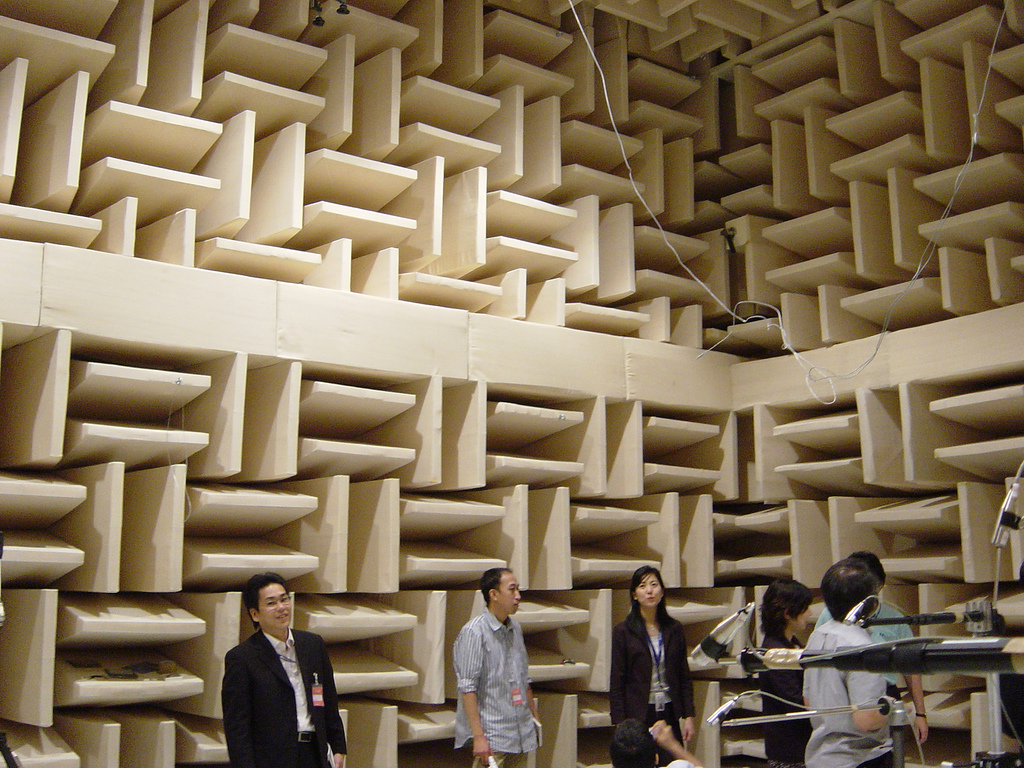
\includegraphics[width=0.6\textwidth]{img/ibm-anechoic.jpg} 
%\captionsetup{justification=centering}
\caption{IBM Anechoic Chamber - wikimedia commons}
\label{fig:ibm-anechoic}
\end{figure}

\subsection{HRIRs}\label{subsec:hrirs}

An important aspect of spatialization in the musical domain, in addition to horizontal and vertical direction of sounds, is the distance of the event in relation to listener. For these three critical localization parameters - those being horizontal position, vertical position, and distance - various associated auditory mechanisms exist in the acoustic domain which facilitate our ability to place sources in space. 

In \textit{near-field} conditions, \textit{auralization} systems - systems that seek to replicate natural phenomena via digital means - tend to model distance as an independent characteristic of directional acoustic propagation. A common definition of \textit{near-field}, albeit informal, is: anything within arms reach, or between 0.5m and 1m (\cite{Betbeder.2017})\footnote{1-2m is the typical distance for HRTF measurements.}. The idea behind this formal separation of near and far field is to exploit "tricks" in sound system design which help simulate real-world acoustic conditions at a much lower computational cost. By analyzing real-world acoustic snapshots, taken with microphones as \textit{impulse responses} (IR) we can observe that many acoustic spaces exhibit similar behaviors, statistically, in particular regions of their \textit{impulse responses}. 

Any acoustic space can be considered a linear time-invariant (LTI) system which can be characterised by a single \textit{impulse response}, much like any other digital filter. Subtle changes in air pressure, based on temperature for example, can affect sound propagation, but for all intents and purposes, this theory holds true. Inside this \textit{near-field} the abundance or lack of reverberant sound, caused by reflections from surfaces, can contribute to our perception of sound distance. However, it is more common to model the \textit{diffuse-field} attributes independently, and use a complimentary system, based on \textit{free-field} plus \textit{near-field} techniques, for horizontal and vertical \textit{auralization}.

Within this particular context, our free/near field condition, we are concerned with impulse responses not of a single omni-directional acoustic sensor, for spatialization systems, but rather with the analysis of two impulse responses - ideally captured at the listeners ears. For this purpose there exist various methodologies for capturing the aforementioned impulse response commonly referred to as \textit{binaural impulse responses} (BIRs) or \textit{Head Related Impulse Responses} (HRIRs), in the time domain\footnote{When these are taken in diffuse-field conditions they are also sometimes called Binaural Room Impulse Responses (BRIRs).}. The most common technique involves placing two small microphones, or \textit{in-ear} microphones, inside a persons ears, and taking snapshots at as many positions as possible by sending \textit{exponential sinusoidal sweeps}\footnote{One among various IR capture methods including: balloon pops, MLS, and linear sinusoidal sweeps.} from speakers surrounding the listener. 

The recordings are then \textit{de-convolved} in order to obtain the effect only of the listeners head and body on the two recordings, as a function of direction. When the excitation signal is perfectly known, de-convolution yields an impulse response which captures the effects of the: room, speaker and microphone. A full-spectrum signal is required for a good IR to be obtained. We tend to use \textit{flat} frequency microphones and speakers, and an anechoic chamber, which has no response, to isolate the effects of head and torso on the incoming signals.

\begin{figure}[ht!]%force figure here, top, strict
\centering
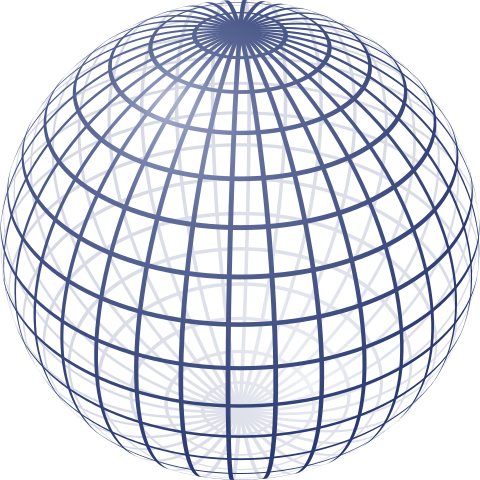
\includegraphics[width=0.3\textwidth]{img/sphere-png.png} 
%\captionsetup{justification=centering}
\caption{Sphere - wikimedia commons}
\label{fig:sphere}
\end{figure}

Figure \ref{fig:sphere} shows a spherical grid, included here to facilitate visualization of the proposed acoustic system. Consider a speaker at each junction between two lines and a listener with \textit{in-ear} microphones in the center of the sphere. The acoustic sampling of the sphere, in the \textit{binaural} sense, will take place by taking \textit{impulse responses} with each speaker, two at a time - one for each ear. This complete set of HRIRs, taken in \textit{free-field} conditions, such as inside our \textit{anechoic chamber}, contain time, level and spectral differences used by our auditory system to localize sound. 

Each of these individual characteristics of each HRIR has a particular name. \textit{Inter-aural level difference} (ILD) refers to the overall energy difference between the two IRs, \textit{inter-aural time difference} (ITD) refers to the time offset, or phase delay, between measurements. Based on the \textit{diffraction}\footnote{Diffraction refers to sounds ability to bend around objects. This is especially true for low frequencies.} and \textit{reflection}\footnote{Reflection refers to sounds ability to bounce off objects. This is especially true for high frequencies.} effects caused by the geometry of the human head, the HRIRs will also exhibit spectral differences, which can be used to discern directions in situations when ITDs and ILDs are not sufficient. ILDs are typically caused by the \textit{shadowing effect} of the head and are therefore frequency dependent (\cite{cuevas20193d}). In other words, the ILD will be greater for higher frequencies since lower frequencies diffract, or bend, around the head, while high-frequencies reflect off the head. 

\subsection{Localization Errors}

Many terms have been defined in the psyscho-acoustic community to describe common occurrences in auditory experiments. Our ability to localize sounds is greatly dependent on the nature of the acoustic environment, as well as the frequency content of the sound source. In addition, we should remember that in the real world, more often than not, multiple sound sources will be present at the same time, making localization tasks more difficult still.

\begin{figure}[ht!]%force figure here, top, strict
\centering
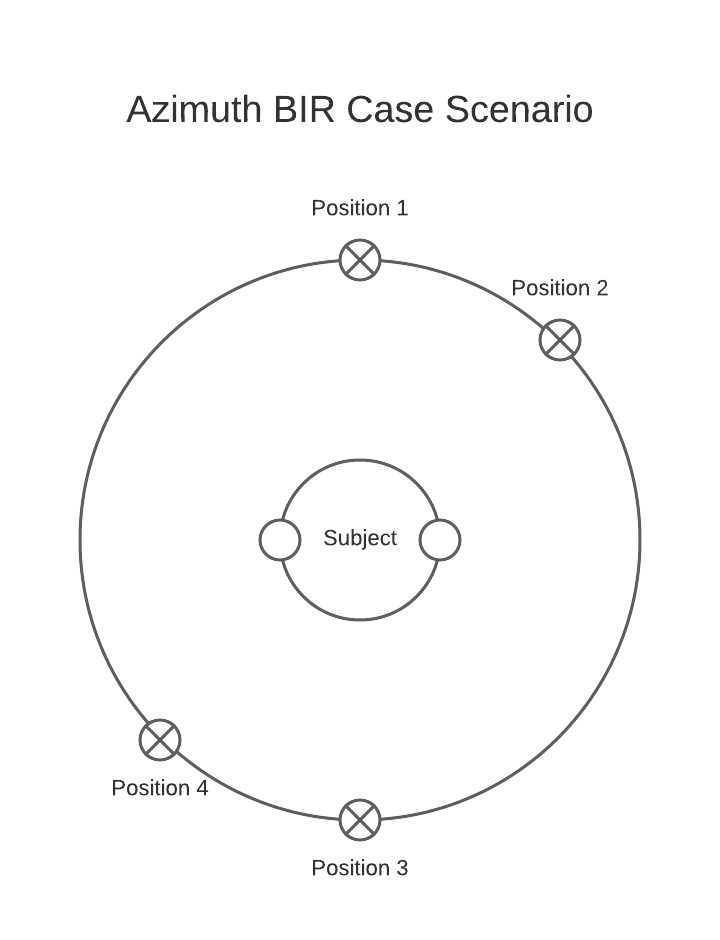
\includegraphics[width=0.5\textwidth]{img/azimuth-bir.png}
%\captionsetup{justification=centering}
\caption{Azimuth BIR Case Scenario}
\label{fig:azimuth-bir}
\end{figure}

In order to demonstrate some common localization errors, we present figure \ref{fig:azimuth-bir}. Consider positions 1 and 3 the figure. Clearly these two positions on the \textit{transverse} plane, otherwise known as the horizontal plane, have identical ILDs and ITDs since the distance from both positions to the subject's ears is identical. Therefore, the subject will only be able to rely on spectral differences to localize the impinging sound. Our outer ear, or \textit{pinna}\footnote{Also called the auricle in some medical textbooks.}, blocks high frequencies arriving from behind the listener acting as low-pass filters. The HRIRs capture all these time and frequency differences in order to simulate directionally-dependent sound propagation via convolution of the associated IRs. 

In contrast, differentiating between positions 2 and 4 should be substantially easier, since we see that the ITD and ILD differences will compliment spectral changes giving us additional information. Assuming the subject is facing position 1, the distance between position 2 and the subjects right ear, the \textit{ipsilateral} ear\footnote{The ear closest to the source.}, will be smaller than the distance to the \textit{contralateral} ear\footnote{The ear furthest away from the source.}. Sound propagates in air at a rate of around 343 m/s and as it travels it loses energy due to friction between molecules according the inverse-square law\footnote{The inverse square law states that with every doubling of distance away from the sound source, the sound will be four times less intense.}. 

\begin{figure}[ht!]%force figure here, top, strict
\centering
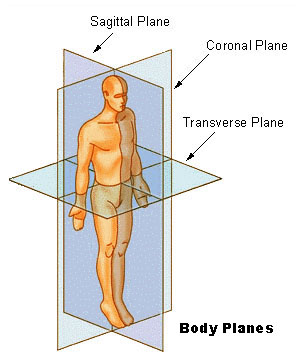
\includegraphics[width=0.5\textwidth]{img/body-planes.jpg}
%\captionsetup{justification=centering}
\caption{Body Planes \cite{body_planes_pic}}
\label{fig:body-planes}
\end{figure}

This additional distance results in a time delay between IRs, as well as level differences. However small these differences might seem, they are crucial for discerning the position of sounds in space. The inability of listeners to differentiate between two sources with identical ITDs and ILDs, that is: any two sources mirrored over the coronal plane\footnote{Also called the frontal plane.}; is called \textit{front-back confusion}. The same principle applies to sources mirrored over the \textit{transverse plane}\footnote{Also called the horizontal plane.}, these errors are called \textit{up-down confusions}. Sources mirrored over the \textit{mid-sagittal}\footnote{Also known as the longitudinal or median plane.} should be easily discerned since ILDs and ITDs will be quite large.  

The human auditory system has been shown to be extremely sensitive. The ITD for a typical human head can vary between $\pm$750$\mu$s. Humans can detect ITDs as low as 10-20$\mu$s which correspond to about 1\textdegree in the horizontal plane (\cite{hacihabiboglu2017perceptual}). ITDs are commonly held as the primary localization cues for low frequencies, while ILDs are more prominent for high frequency signals. 

\begin{figure}[ht!]%force figure here, top, strict
\centering
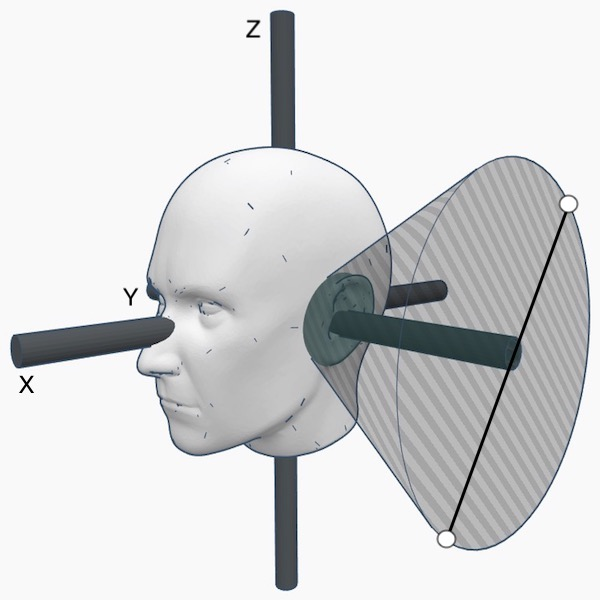
\includegraphics[width=0.5\textwidth]{img/cone_confusion.JPG}
%\captionsetup{justification=centering}
\caption{Cone of Confusion}
\label{fig:cone-confusion}
\end{figure}

The \textit{cone of confusion} is yet another term used to describe a phenomenon generally experienced in localization experiments. Consider the two white dots on the circumference of the cone depicted in figure \ref{fig:cone-confusion}. The two positions, much like any two dots directly opposite each other on this circle, will have identical ITDs and ILDs because their respective distances to the \textit{contralateral} and \textit{ipsilateral} ears, will be the same. In this cases, spectral differences become critical to differentiate between sources. When ambiguous localization tasks arise, small head movements often help resolve source positions.

Our ability to localize sources is most accurate in the horizontal plane. Psycho-acoustic experiments have revealed that \textit{localization blur}, the inability for listeners to discern the direction of a sound, is generally less than 10\textdegree for horizontal sources, but around 20\textdegree for sources in the median plane (\cite{hacihabiboglu2017perceptual}). Two associated objective measures are the \textit{Minimum Audible Angle} (MAA) and the \textit{Minumum Audible Movement Angle} (MAMA). The MAA, a formal term used to quantify \textit{localization blur}, is the minimum detectable angular difference of two successive sound sources \cite{reardon2017evaluation}. The MAMA, is the smallest arc that a moving source must travel to be discriminable from a stationary source \cite{moore1995hearing}.

\subsection{Perception of distance}

Perception of distance is more complex in some ways than that of orientation. \cite{zahorik2005auditory} provides, a comprehensive overview of auditory distance perception research, including some cognitive research which examines brain response to acoustic stimuli. As aforementioned, there are several cues that affect our perception of distance - the most salient one being overall energy. A few other unmentioned cues, however, also affect our perception of distance. Among these, is the absence, or presence, of high frequency content in a signal. High frequency signals tend to dissipate faster in air than low frequency ones, because of the additional friction between molecules inherent to these acoustic events. 

\textit{Auditory parallax}, the effect whereby the position or direction of an object appears to differ when heard from different positions, has also been shown to improve distance estimations. Finally, as mentioned before, familiarity tends to affect our perception of sound origin. A sample of a whispering voice, virtually placed far away, will appear closer than it really is. Adversely, a shouting voice, placed close, will appear to be further away than reality.

Finally, \textit{interaural coherence} (IC), is the measured statistical coherence of signals received at each ear. In a \textit{diffuse field}, IC is low, because the scattering of sounds off walls interact in unpredictable ways, which result in some amount of randomness in the signals when compared to each other. Therefore, IC can be used as a statistical estimate of distance since we can assume that in most real-world conditions sound sources will be diffused acoustically lowering the overall IC for distant sources more than those proximal.

\subsection{Precedence effect}

\textit{Summing localization} is a phenomenon - primarily based on ITD - which affects of perceived direction-of-arrival of sounds. When a broadband signal - a signal with broad range of frequencies present - is played from two directions with a small delay of less than 1 ms, a single event is perceived at the direction between sources. The perceived location shifts towards the first played source, as the delay increases. This \textit{fusion} is one of three characteristics of the \textit{precedence effect}, also known as the \textit{Law of First Wavefront} or \textit{Haas effect}, described in 1949 by Helmut Haas. When the delay is between 1 and 5ms, a single event close to the leading source can be heard \cite{hacihabiboglu2017perceptual}. The lagging source - the delayed copy of the sound - can be perceived due to the change in timbre, and is essentially equivalent to a feedforward comb filter where the delayed copy is played back over a second discrete channel. Within this context the \textit{echo threshold}, refers to the amount of delay that must be introduced to the copy before we begin perceiving the two sounds as independent non-fused events. This threshold is dependent on the nature of the signal. For a short broadband click, 5 ms might be enough to create an echo. For music and speech signals, the threshold is longer, and can be as high as 20 ms.

The precedence effect can be summarized by the following three phenomena: 

\begin{enumerate}
    \item \textit{Localization dominance}: the direction of an auditory event depends predominantly on the leading source.
    \item \textit{Fusion}: a single auditory event is perceived when two sound events are below the \textit{echo threshold}.
    \item \textit{Lag Discrimination Suppression}: the direction of the lagging sound is suppressed.  
\end{enumerate}

\subsection{Doppler Shift}

\textit{Doppler shift} is another auditory cue, related to \textit{auditory parallax}, which can aid in our estimation of source distance and direction. Doppler shift is the phenomenon we experience when we perceive the pitch of an ambulance's siren change as it approaches and moves away from us. Specifically, as the siren moves towards us, the pitch seems to increase, and as it moves away, it seems to decrease. \cite{lavalle2016virtual} provides a whole chapter on the auditory mechanisms involved in Virtual Reality (VR). The book covers the fundamentals of optics, interaction, and tracking, and is recommended for anybody interested in Extended Reality (XR). Equation \ref{eq:doppler}, from chapter 11, describes our perceived frequency of sound as a function of it's velocity. By combining this auditory cue with distance based intensity dampening we can realistically simulate moving sources.

\begin{equation}
f_{r}=\left(\frac{s+v_{r}}{s+v_{s}}\right) f_{s}
\label{eq:doppler}
\end{equation}

Where: 
\begin{enumerate}
    \item $f_r$ is the resulting frequency.
    \item $s$ is the speed of sound (343.2 m/s roughly at C 20\textdegree).
    \item $v_r$ is the velocity of the receiver (negative if receiver is moving away). 
    \item $v_s$ is the velocity of the source (negative is the source is moving away).
    \item $f_s$ is the original frequency of the source.
\end{enumerate}

\subsection{Binaural Synthesis Errors}

Of particular importance to our work is the use of binaural synthesis for the simulation of acoustic spaces. Binaural synthesis allows us to experiment with \textit{spatial music} without the need for sophisticated and often inaccessible loudspeaker systems. In binaural synthesis, sound sources are \textit{convolved}\footnote{Convolution of a source with an impulse response if equivalent to applying a filter.} with HRIRs dynamically to simulate surround sound experiences. Binaural synthesis has become increasingly popular with the growth of \textit{extended reality} (XR) systems. Several problems, such as: personalized HRTFs, externalization problems, and localization errors; persist. 

Poor \textit{externalization}\footnote{Also sometimes refered to as Inside-the-Head Locatedness (IHL).}, the degree to which listeners perceive sources as originating inside their head, can be mitigated by the use of a head-tracking system. The systems, based on \textit{inertial measurement units} (IMU), monitor the orientation of the listener and adjusts the soundfield accordingly - ideally in real-time. When no rotation adjustment is included, our auditory system assumes that sources must be originating from inside our head, as this is the only rational conclusion for sources without dynamic filtering based on BIRs. The subtle spectral changes from location to location, provided by head-tracking, provide a way to disambiguate between source positions. The addition of diffuse field modeling, in the form of reverberation unit, also supports improved \textit{externalization}(\cite{sakamoto1976out}). 

%%%%%%%%%%%%%%

\todo[inline]{This later section will likely be moved to q2 under binaural synthesis}

\cite{cuevas20193d} provides an extensive literature review on the subject of \textit{binaural spatialization}. In this particular text, one of the most comprehensive readings on binaural synthesis, the authors describe the steps undertaken for each part of the "signal chain". Figure \ref{fig:3dti-chain} shows a diagram of the implementation. 

For the \textit{free-field} modeling, an anechoic system based on BIRs/HRIRs is implemented, following:

\begin{enumerate}
    \item Distance-dependent attenuation (inverse square law or acoustic power law), this step also includes far-field distance simulation modeling air impedance (distance-dependent low-pass filtering).
    \item HRIR obtained using \textit{barycentric interpolation} and are ITDs removed to dynamically adjust for different head sizes.
    \item HRIR convolution.
    \item ITD is computed and added to the signals.
    \item ILD correction for \textit{near-field} sources.
    \item Directionality features for hearing aids (if any).
\end{enumerate}

For the \textit{diffuse-field} modeling, an non-anechoic system based on BRIRs is implemented, following:

\begin{enumerate}
    \item Independent distance-dependent attenuation to control the \textit{direct-to-reverberant ratio} (DRR). 
    \item Sources are encoded into 1st Order Ambisonic (FOA).
    \item These channels are convolved with encoded versions of the BRIRs, which have been processed to remove any direct sound.
\end{enumerate}

\begin{figure}[ht!]%force figure here, top, strict
\centering
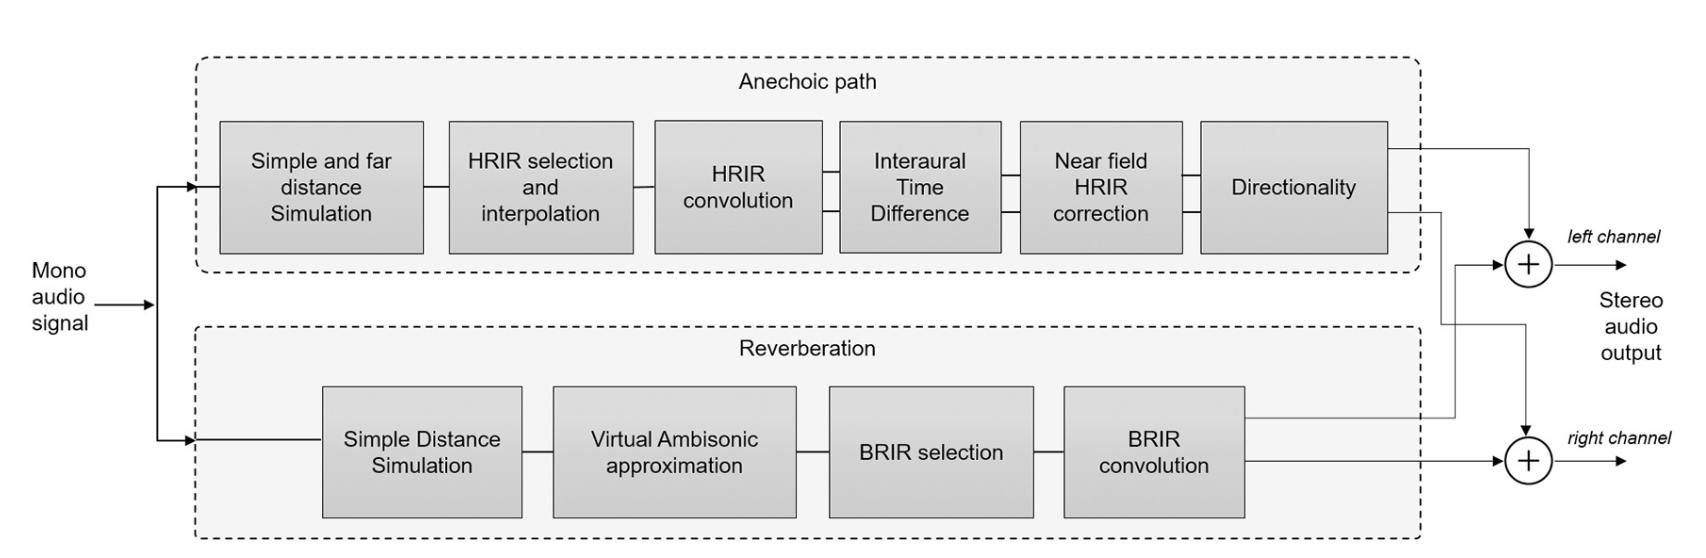
\includegraphics[width=1.0\textwidth]{img/3dti-chain.png} 
%\captionsetup{justification=centering}
\caption{3DTI Toolkit Binaural Structure - \cite{cuevas20193d}}
\label{fig:3dti-chain}
\end{figure}

%free vs. diffuse field

\subsection{Reverberation}
%dont forget to talk about room acoustics. T60, etc. Sabine equation. RT60. 

%near, far



%https://books.google.com.bo/books?id=OywDx9pxCMYC&pg=PA1&source=gbs_toc_r&hl=es-419#v=onepage&q&f=false






\section{Conclusion}
%spatial music  (live) [CREATION]
\chapter{Spatial Music: Past, Present and Future} \label{ch:spat-mus} 

\section{Introduction}
%This chapter will be developed with Professor Tom Erbe.

This chapter deals with spatial music, a genre of music in which space forms a primary aesthetic element of the composition. We will discuss how spatial music has developed over the course of human history, talk briefly about some of the composers that broke ground by pioneering compositional techniques in this field, and, finally, discuss modern approaches to spatial music by composers such as: Hagan, Lyon, Lopez-Lezcano, Barrett, and many more. 

We will also discuss spatial instruments, which refer to instruments which have considered the manipulation of sound in space as a critical parameter of the instrument design. In contrast to traditional instruments which assume sound radiates outwards from the acoustically activated object, these instruments might not produce any sounds by themselves, and instead work in conjunction with computers, which receive data in order to synthesize sound at various real or \textit{phantom} speakers, also known as virtual speakers. 

These instruments are not always entirely electronic - at times we encounter designs in which traditional instruments have been extended via the use of sensors to give the performer control over the location of provenance of the sound. Often, computer musicians inextricably tie the development of instruments, or systems, to their compositions in ways that blur the line between: software and score, instrument and composition, or method and material. Some of these \textit{aesthetics} will also be discussed in this chapter. 

Finally, we will discuss the likely direction of spatial music in the future. Spatial audio algorithms have been already thoroughly researched for many years. It appears on some level that many of the questions composers sought to ask regarding these systems have already been answered by these various developments. This final section will therefore consider how other technologies might be used in the future towards compositional means based on state-of-the-art research in computer music. 
%Music Information Retrieval (MIR) and robotics. 

\section{History of Spatial Music} \label{sec:hist_spat_mus}

\subsection{Acoustic Music} \label{subsec:acoustic_mus}

\todo[inline]{Boren's chapter has more info that could be incorporated into this section.}

\textit{Antiphonal} music is perhaps the oldest spatial music tradition. The practice of \textit{antiphonal} music, also known as \textit{call and response}, can be traced back to Biblical Times, with evidence of its existence as far back as the Roman Catholic Church in the 4th century. In a call and response system, the composer writes melodic lines using tension and resolution having independent choral group assigned different parts of the melody. The composer might create tension by using a dissonant note as the final note of the calling phrase. A different group, located in a different location of the stage, would resolve the melodic phrase - usually ending in the tonic of the scale, while the harmony resolves using some traditional cadence\footnote{Like a IV-I, plagal cadence, or a V-I, perfect cadence.}. 

Many of these early works are hard to replicate today due to the lack of documentation. In the 16th century, however, printed works in spatial music would surface. Some of these initial innovative pieces were written by the Flemish composer Adrian Willaert\footnote{Netherlandish composer of the Renaissance.}, for example, whom exploited the \textit{Basilica de San Marco's\footnote{The cathedral church of the Roman Catholic Archdiocese of Venice, northern Italy.}} two organs in antiphonal compositions featuring two separate choirs and multiple instrumental groups \cite{arnold1959significance}. The technique \textit{cori spezzati}, or separated choirs, was re-introduced in his 1550's piece titled \textit{Vespers}, which itself featured multi-part arrangements and echo effects. Willaert's pupil, Andrea Gabrieli, an Italian composer of the late renaissance, would later continue his teacher's work, cementing spatial music as a hallmark of the Venetian musical practice. 

\begin{figure}[ht!]%force figure here, top, strict
\centering
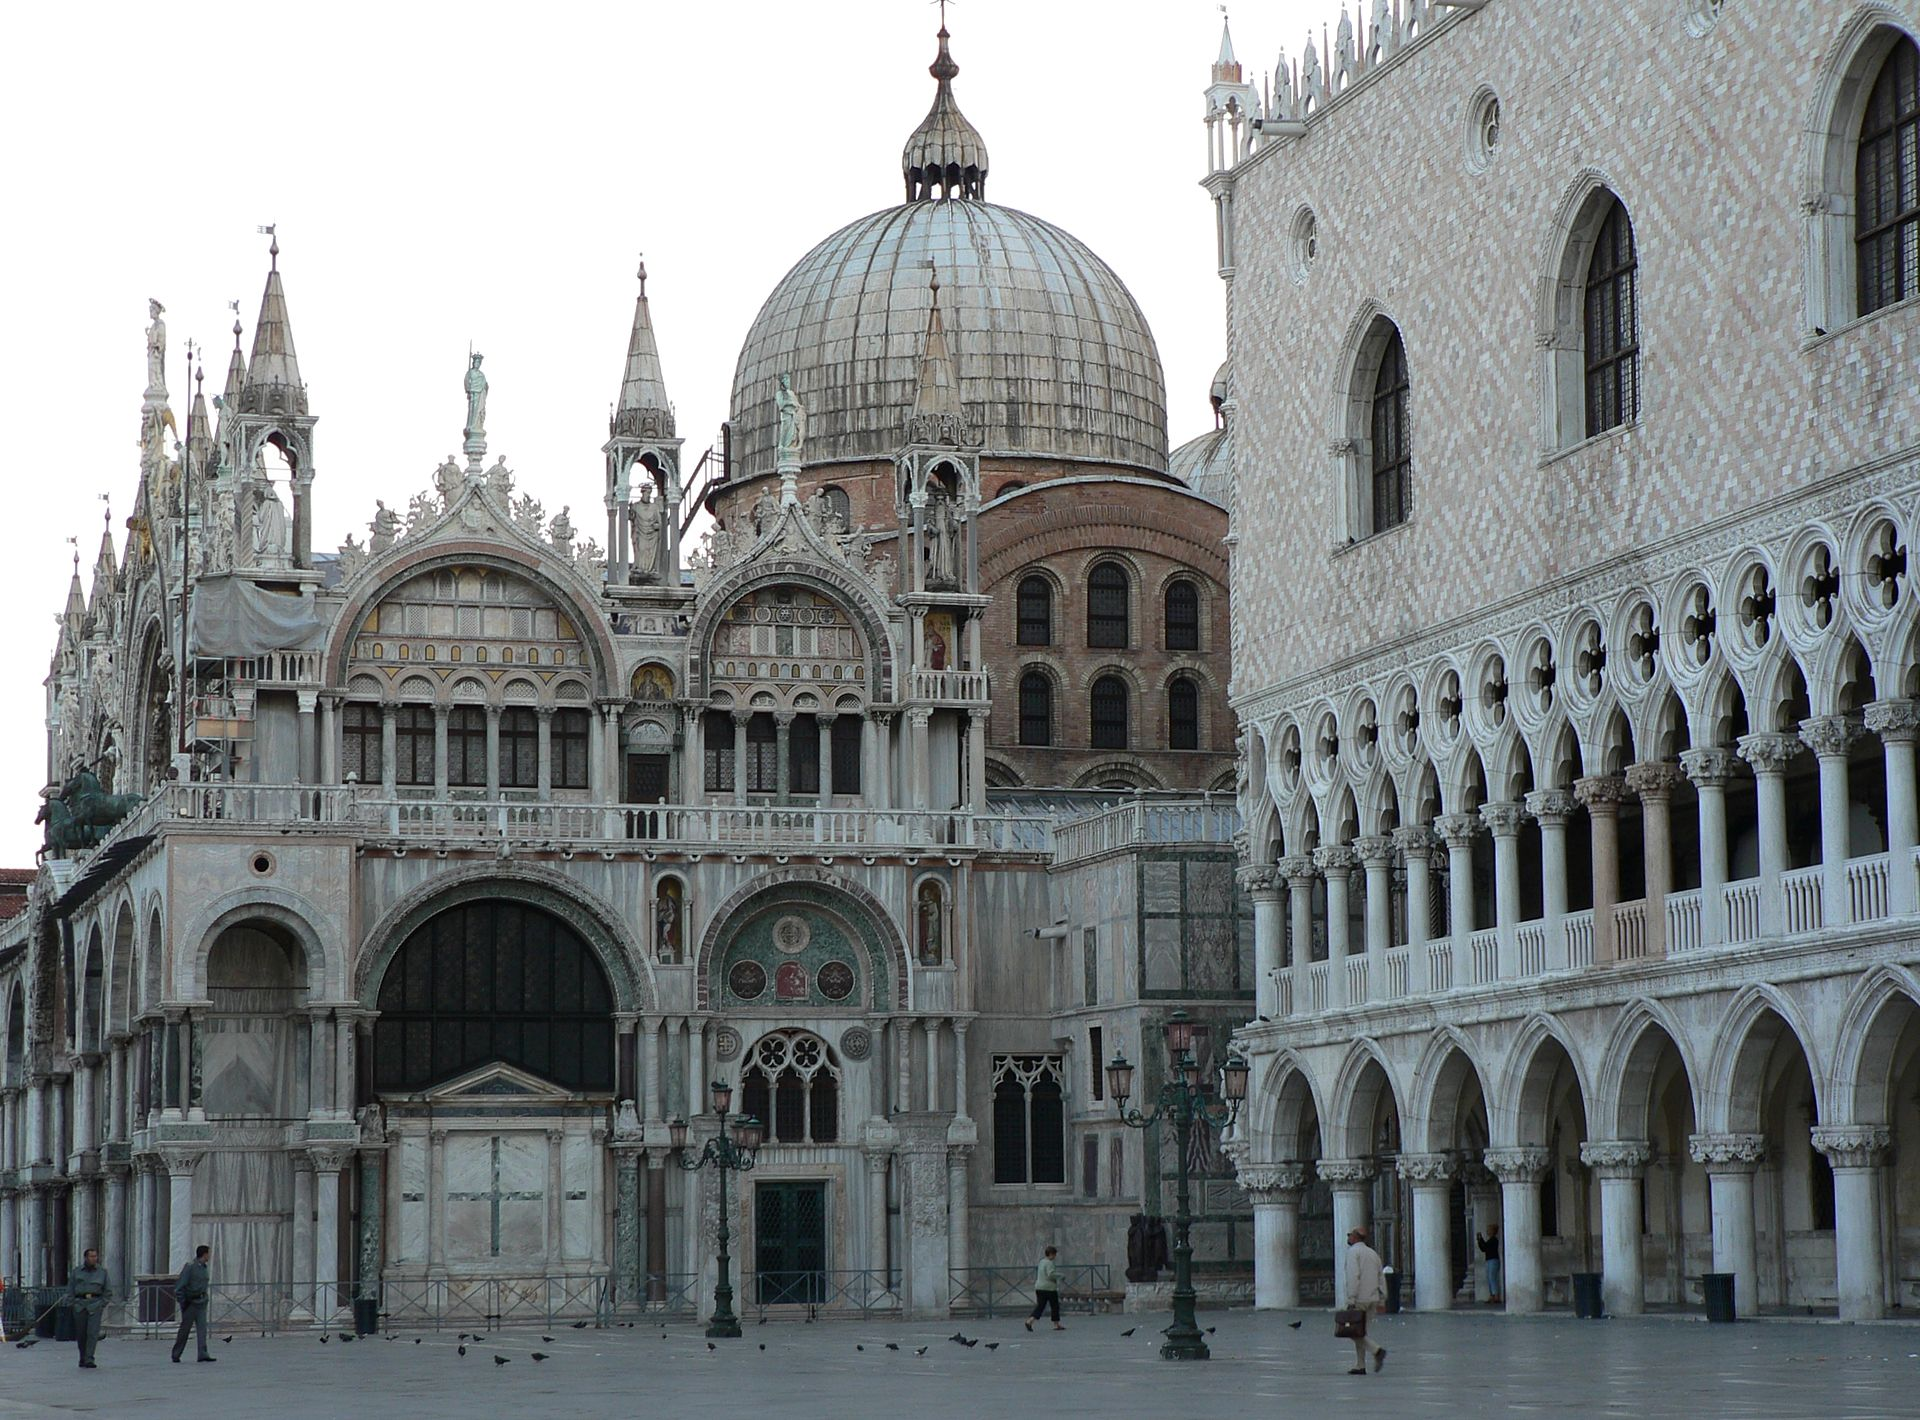
\includegraphics[width=0.7\textwidth]{img/basilica-san-marcos.JPG} 
%\captionsetup{justification=centering}
\caption{Basilica de San Marco \cite{Venbasil3:online}}
%license: cc by sa 3.0
\end{figure}

As a result of Willaert's work the practice of spatial music quickly spread to other parts of Europe where it was quickly adopted by composers such as Thomas Tallis in England. \textit{Spem in alium}, one of Tallis's most famous pieces, was composed for Queen Elizabeth upon her 40th birthday, in 1573, and featured 40 vocal parts arranged in eight 5-voice choirs. The high point of spatial music during the baroque era might however be Orazio Benevoli's\footnote{Franco-Italian composer born in Rome (19 April 1605 – 17 June 1672).} \textit{Festival Mass}, written in 1628 for the \textit{Salzburg Cathedral} which called for 16 vocal parts, 34 instrumental parts, two organs, and a basso continuo\footnote{Figured bass where the most common combination is harpsichord and cello for chord and bass-line respectively.} \cite{zvonar1999history}.

Following the baroque era, interest in spatial music subsided until the beginning of the Romantic period. A key distinction of this era is the use of spatial music for theatrical effect. The romantic period is often characterized by the rise and popularity of operas by composers such as: Hector Berlioz, a French Romantic composer and conductor (11 December 1803 – 8 March 1869) who wrote \textit{Requiem} in 1837, and Gustav Mahler, an Austro-Bohemian Romantic composer (7 July 1860 – 18 May 1911)\footnote{Considered one of the leading conductors of his generation.} who wrote \textit{Symphony No.2} in 1895 \cite{einstein1948music}. These composers not only spaced instruments for their performances but also choreographed the entrance and exiting of musicians as they played, creating some iconic musical moments.

In the 20th century, experimentalists such as Charles Ives, American modernist composer (October 20, 1874 – May 19, 1954), and Luigi Russolo, Italian Futurist composer and the author of the manifesto \textit{The Art of Noises} (30 April 1885 – 6 February 1947), inspired by the tumultuousness of industrial life, refined the art of musical collage using spatial sound \cite{jones199120th}. Ives's 1908 \textit{The Unanswered Question} called for offstage strings. Charles was inspired by his father George, a Civil War bandmaster, and music teacher, who had himself experimented with spatial music in his days. 

Henry Brant\footnote{Canadian-born American composer whom composed numerous orchestral spatial works (September 15, 1913 – April 26, 2008).}, inspired by Ives's music, would go on to create \textit{Antiphony I} (1953) which called for five spatially separated orchestras, and, \textit{Voyage Four} (1963) which called for three conductors to direct: percussion and brass on stage, violins on one balcony, violas and celli on another, basses on the floor level at rear, woodwinds at a rear balcony, and several performers in the audience \cite{zvonar1999history}. Brant's \textit{Windjammer} (1969), likely inspired by the opera composers of the baroque times, featured a static horn soloist and several wind players that moved along prescribed routes as they performed, in a choreographed manner. 

\cite{harley1997american} provides a rich analysis of four of Brant's most important works in the field of spatial music. Brant emphasized the need for differing timbres to be represented in his music, since he believed the heterogeneity would aid in the clarity of the musical representation. Indeed, if multiple instruments of the same family were spatially distributed, it would be difficult to differentiate melodic phrases, especially if these were all playing in the same register. 

% Brant summarized his main observations with regards to spatial composition in a 1967 articles paraphrased as following: 
% \begin{enumerate}
%     \item \textbf{Spatial separation clarifies texture}: when multiple musicians play different musical phrases in the same octave range, separating them spatially helps give clarity to each stream. 
%     \item \textbf{Separate groups are difficult to coordinate}: exact rhythms might be difficult to accomplish due to the distance it takes for sounds to arrive from one playing position to the next. 
%     \item \textbf{Spatial separation is equivalent to range separation}: it is possible to enhance the texture of a melodic phrase simply my separating musicians playing the same material.  
%     \item \textbf{Spatial arrangements must allow flexibility}: the specific architectural demands of the works cannot always be met, alternatives should be provided whenever possible.
% \end{enumerate}

Brant is perhaps one of the mos prolific composers of spatial acoustic works with a repertoire of 67 spatial pieces. Brant also wrote extensively on the subject of spatial music and experimented at length with form, rhythm and perceptual experience in this context. In contrast to other composers of his era, Brant's music dealt exclusively with acoustic means, which he creatively articulated to provide depth, envelopment and movement.  

\todo[inline]{There are still more works by Brant that might warrant mentioning.}

\subsection{Electro-acoustic Music} \label{subsec:elec_acoustic_mus}

Along a parallel branch of history there exist a number of musical experiments conducted in the 20th century by avant-garde musicians and composers typically categorized as \textit{electro-acoustical}. This label is used to separate them from traditional composers who avoided electronics or seldom exploited electronics in their compositions. The composers of this space and time were all activated by the development of sound recording, radio and telephony, and used them purposefully in their works. With the possibility of sound as a medium displaced from its source, dozens of new forms of music were created.

The birth of recorded sound brought along an era of technological music development featuring composers and engineers striving to encourage audiences to attend live events. Thaddeus Cahill's (1900-1906) \textit{Telharmonium} (1897) is considered the first electrical musical instrument of its kind \cite{bode1984history}. Also known as the Dynamophone, this electrical organ, which employed additive synthesis, was used to deliver music to homes on a subscription basis via a telephone line. We should note here that the element of space is present in an example such as this one, in a different semantic context, given the distance created between performer and audience. This device was in part inspired by Clement Ader's \textit{Théâtrophone} (1881), which sent stereo signals of actors via telephone wires \cite{TheTelh3:online}.

\begin{figure}[ht!]%force figure here, top, strict
\centering
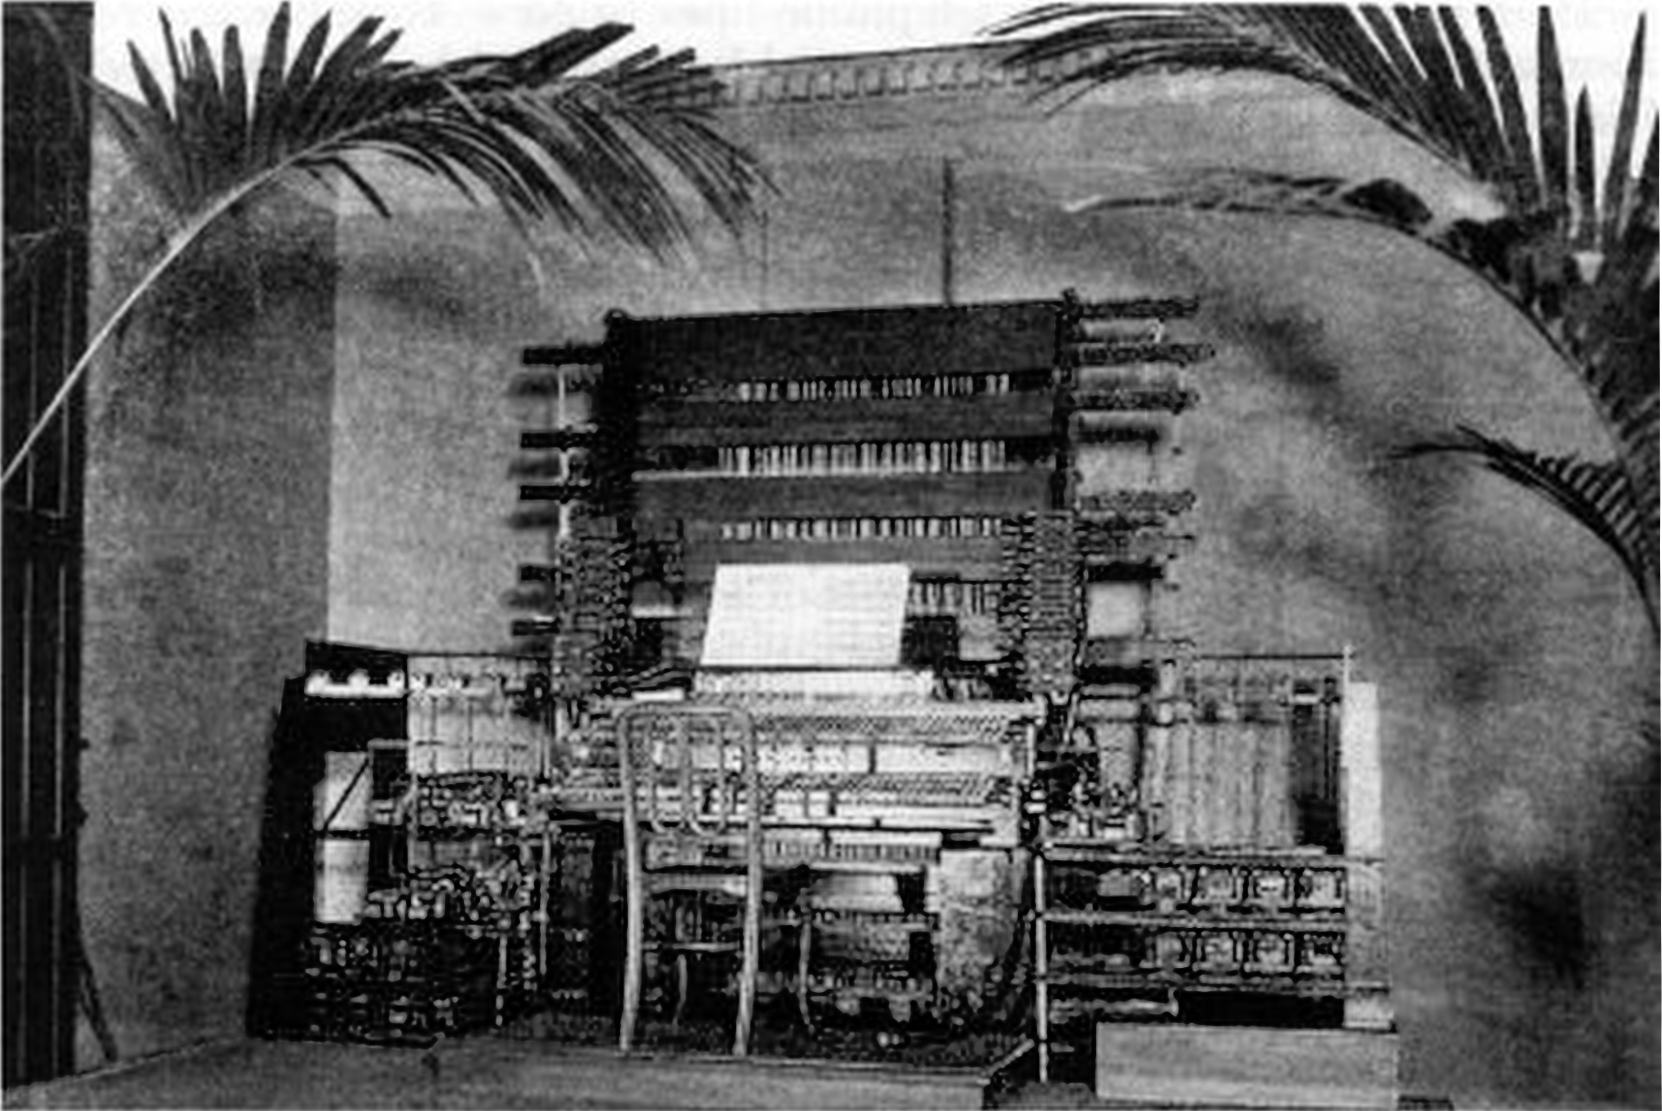
\includegraphics[width=0.8\textwidth]{img/telharmonium.jpg} 
%\captionsetup{justification=centering}
\caption{Telharmonium \cite{Telharmo82:online}}
%license: public domain
\end{figure}

Later, in 1923, Leon Theremin would introduce a new instrument to the public. The \textit{theremin}, named after its inventor, used two antennae to control the pitch and volume of a synthesizer. The user must position their hands in space to control the instrument and produce the desired sound. Theremin later formed ensembles in which multiple theremin were used in one of the first public displays of multi-channel loudspeaker music ever. The theremin is another particularly provoking example as it illustrates not only how space can be used for acoustic effect, but ergonomically speaking, it shows how an instrument can use space to facilitate its playing. Neither of these two instruments, however, exploit psycho-acoustic principles, the development of such instrument would come later. %spatial instrument

\begin{figure}[h!]%force figure here, strict
\centering
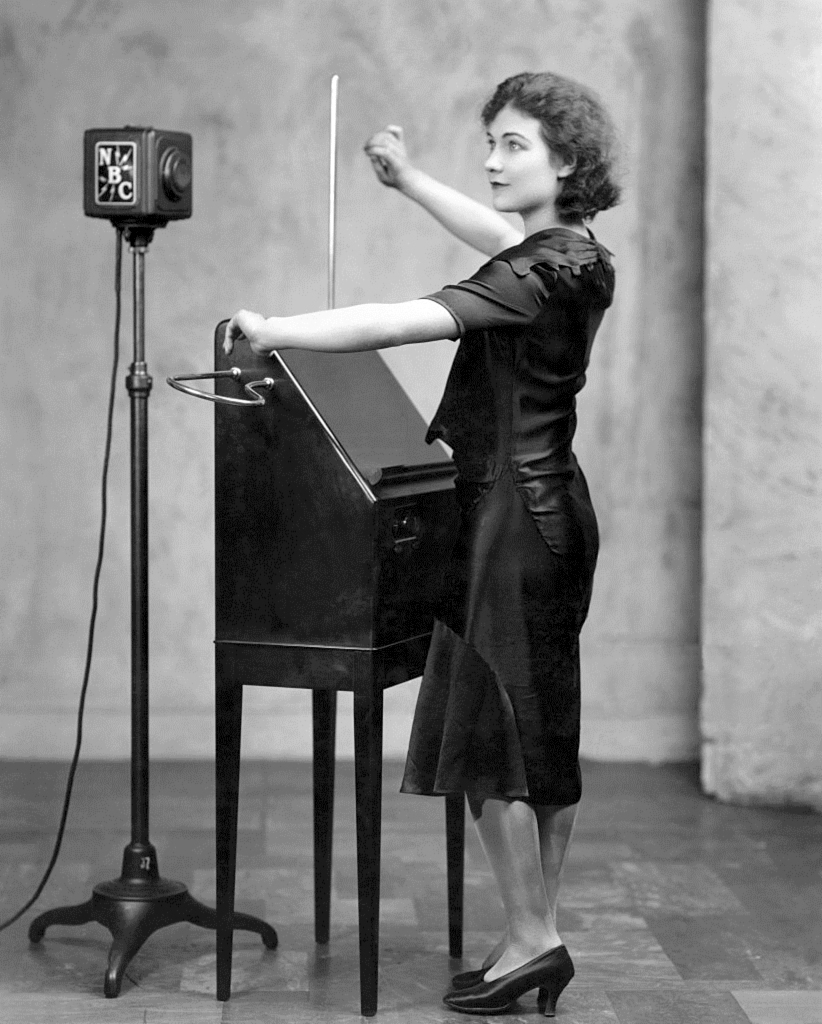
\includegraphics[width=0.5\textwidth]{img/theremin.jpg} 
%\captionsetup{justification=centering}
\caption{Alexandra Stepanoff\protect\footnotemark playing the theremin on NBC Radio, 1930 \cite{Theramin45:online}}
\end{figure}

\footnotetext{Alexandra Stepanoff was one of Léon Théremin’s first theremin students in the United States \cite{2020_stepanoff}.}

The 20th century also saw the rise of phonographs\footnote{Colloquially known as record players.} as musical instruments. Paul Hindemith\footnote{Prolific German composer (16 November 1895 – 28 December 1963).} began this practice in the 1920's and 30's nearly 80 years before DJing practices became popular \cite{manning2013electronic}! John Cage\footnote{American avant-garde composer (September 5, 1912 – August 12, 1992).} also adopted the use of phonographs compositionally in \textit{Imaginary Landscape No. 1} (1939) which used multiple turntables and test tones, and in \textit{Imaginary Landscape No. 4} (1951) where he used 12 radios, 24 performers and a conductor. In addition to exploring the use of phonographs as instruments, Cage also exploited radio broadcast and tape in his creative practice.  

By separating the original performer from the playback these composers were playing not just with space, but also time. Cage, along with a group of experimental composers called "Project for Music for Magnetic Tape", would go on to write four pieces for tape \cite{cage1961experimental} during the 50s. The most famous piece that emerged from the group was likely \textit{Williams Mix}\footnote{\href{http://tre.ucsd.edu/wordpress/?p=644}{Tom Erbe created a Pd version of William's Mix. (access: Jan 7, 2021)} } (1952) which called for 8 tape machines each played back from its own speaker and hundreds of sounds carefully spliced together. This was one of Cage's first use of chance in musical composition. The project also resulted in works by Earle Brown\footnote{American composer who pioneered the use of graphic scores (December 26, 1926 – July 2, 2002).} (\textit{Octet}) and Morton Feldman\footnote{American composer perhaps best known for his extended works which could last up to six hours (January 12, 1926 – September 3, 1987).} (\textit{Intersection}), both using 8 tape players and speakers. 

\begin{figure}[ht!]%force figure here, top, strict
\centering
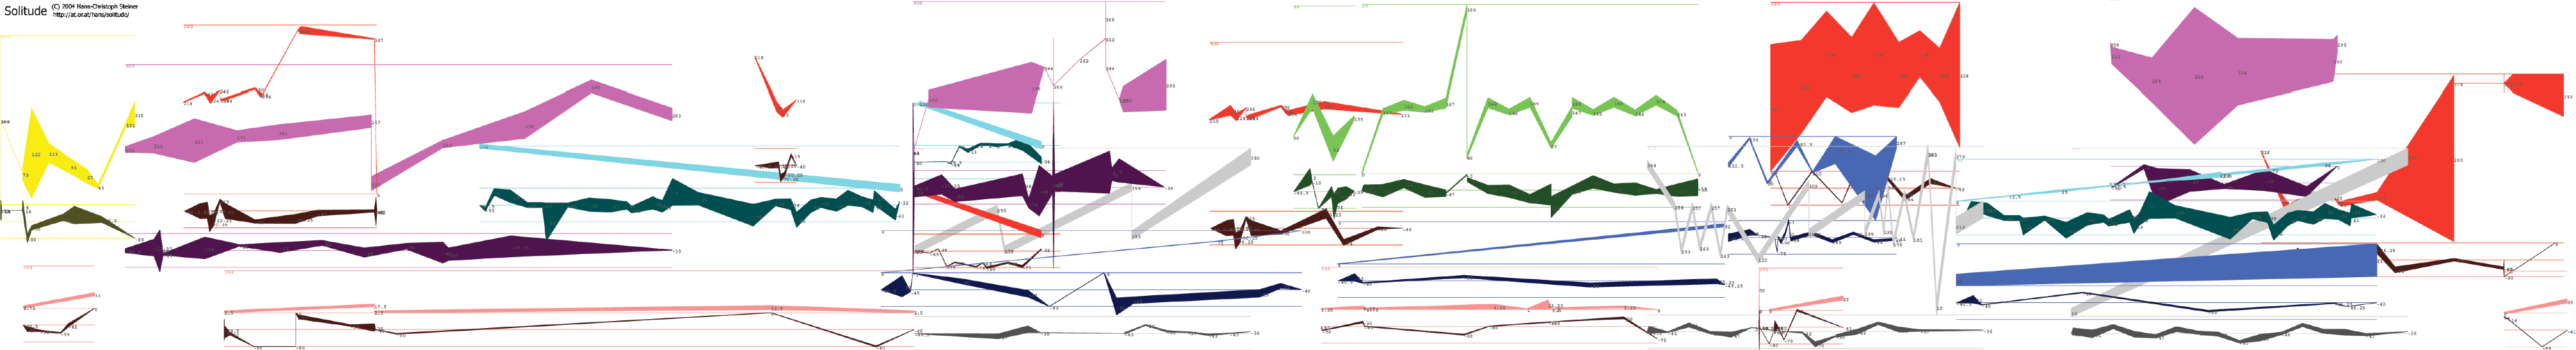
\includegraphics[width=1.0\textwidth]{img/solitude.png} 
%\captionsetup{justification=centering}
\caption{Hans-Christoph Steiner's\protect\footnotemark graphic score for Solitude, created using Pure Data's data structures. An example of a graphic score, such as those popularized by Earle Brown. \cite{wikipedia_2020_graphic}}
\end{figure}

\footnotetext{\href{https://at.or.at/}{Hans-Christoph Steiner's site.}}

Cage, Brown and Feldman were greatly influenced by Pierre Schaeffer, a french engineer at Radiodiffusion-Television Francaise (RTF), who in 1948, presented the first musical works created with disk recorders. These were the first examples of \textit{musique concrète}, a style of music which is defined by the use of recorded sounds interpreted as musical material. Schaeffer would later go on to collaborate with Pierre Henry, another notorious French composer, creating a repertoire of works for tape including, most notably \textit{Symphonie pour un Homme Seul}, which translates to "Symphony for one man alone". (1950). 

In their 1950 piece, four channels were arranged in a tetrahedral\footnote{Three sided pyramid.} configuration with two front speakers, one back speaker, and a final overhead speaker, making this one of the first examples of \textit{periphonic}\footnote{Periphonic refers to sound with height, while \textit{pantophonic} is used to denote sound systems with horizontal-only reproduction.} music. Schaeffer also helped developed the \textit{potentiomètre d'espace}, one of the first \textit{spatial audio} audio controllers which he controlled during live performances to modify the amplitude of speaker feeds. 

In Germany, another composer by the name of Karlheinz Stockhausen was making his mark in \textit{electro-acoustic} music. Stockhausen is perhaps the most ambitious composer of \textit{spatial music} in this era. Inspired by tape music, Stockhausen would travel to RTF, the birthplace of tape-based works, to learn about the technology. Soon after his time at RTF, he would return to Westdeutsche Rundfunk's (WDR) Studio fur Elektronische Musk\footnote{Which translates to studio for electronic music.} to create his most prolific tape pieces. \textit{Gesang der Jünglinge}\footnote{Which translates to "Song of the Youths".} (1956) is considered by some as the first piece for multi-track tape, using a 4-track machine plus a fifth mono tape player for the fifth channel. The premiere featured a number of speakers arranged \textit{panoramically} onstage \cite{zvonar1999history}. Stockhausen later remixed this piece for quadraphonic sound\footnote{Playback system which uses 4 speakers.} system. In 1960, he would go on to create \textit{Kontakte}, his first truly quadraphonic piece. Stockhausen used a turntable system with a rotating speaker and four microphones to create the illusion of spinning sounds. Stockhausen also explored spatial attributes of sound in his acoustic compositions written for multiple orchestras and multiple choruses. His most ambitious and bizarre work is perhaps \textit{Helikopter-Streichquartett} (1993), completed much later. In this piece the four members of a string quartet perform from four helicopters, which fly independent routes, and each have their own audio-visual system, along with a sound engineer. The sound and video is transmitted to the concert hall. The sound from the flying helicopters is also part of the piece \cite{stockhausen1996helikopter}. 

In 1958, another one of the most important examples of spatial electronic music would be performed. Edgard Varèse's\footnote{French-born composer (December 22, 1883 – November 6, 1965). Varèse coined the term "sound mass" to describe his music.} \textit{Poème Électronique} was featured at the Brussels World Fair (Expo 58), a major international event with artists from all over the world. The festival attracted up to two million visitors! For the exposition of this piece, the Philips Corporation set up 15 tape recorder and over 400 loudspeakers \cite{malham19953}. This is still one of the largest spatial music compositions that have ever been accomplished. Xenakis, another giant of electro-acoustic music, designed the Philips Pavilion under the supervision of renowned Swiss-French architect Le Corbusier (1887-1965). Xenakis's \textit{Concret PH}, created using recordings of burning charcoal, modified using tape techniques, also played at the Expo, as an interlude between performances of Varèse's piece, which was the main attraction\cite{valle2010concrete}. Expo 58 also featured \textit{Vortex}, a series of thirteen programs developed by Jordan Belson and Henry Jacobs for the Morrison Planetarium in San Francisco. The program featured music by Stockhausen among many others \cite{zvonar1999history}.

\begin{figure}[h]%force figure here, top, strict
\centering
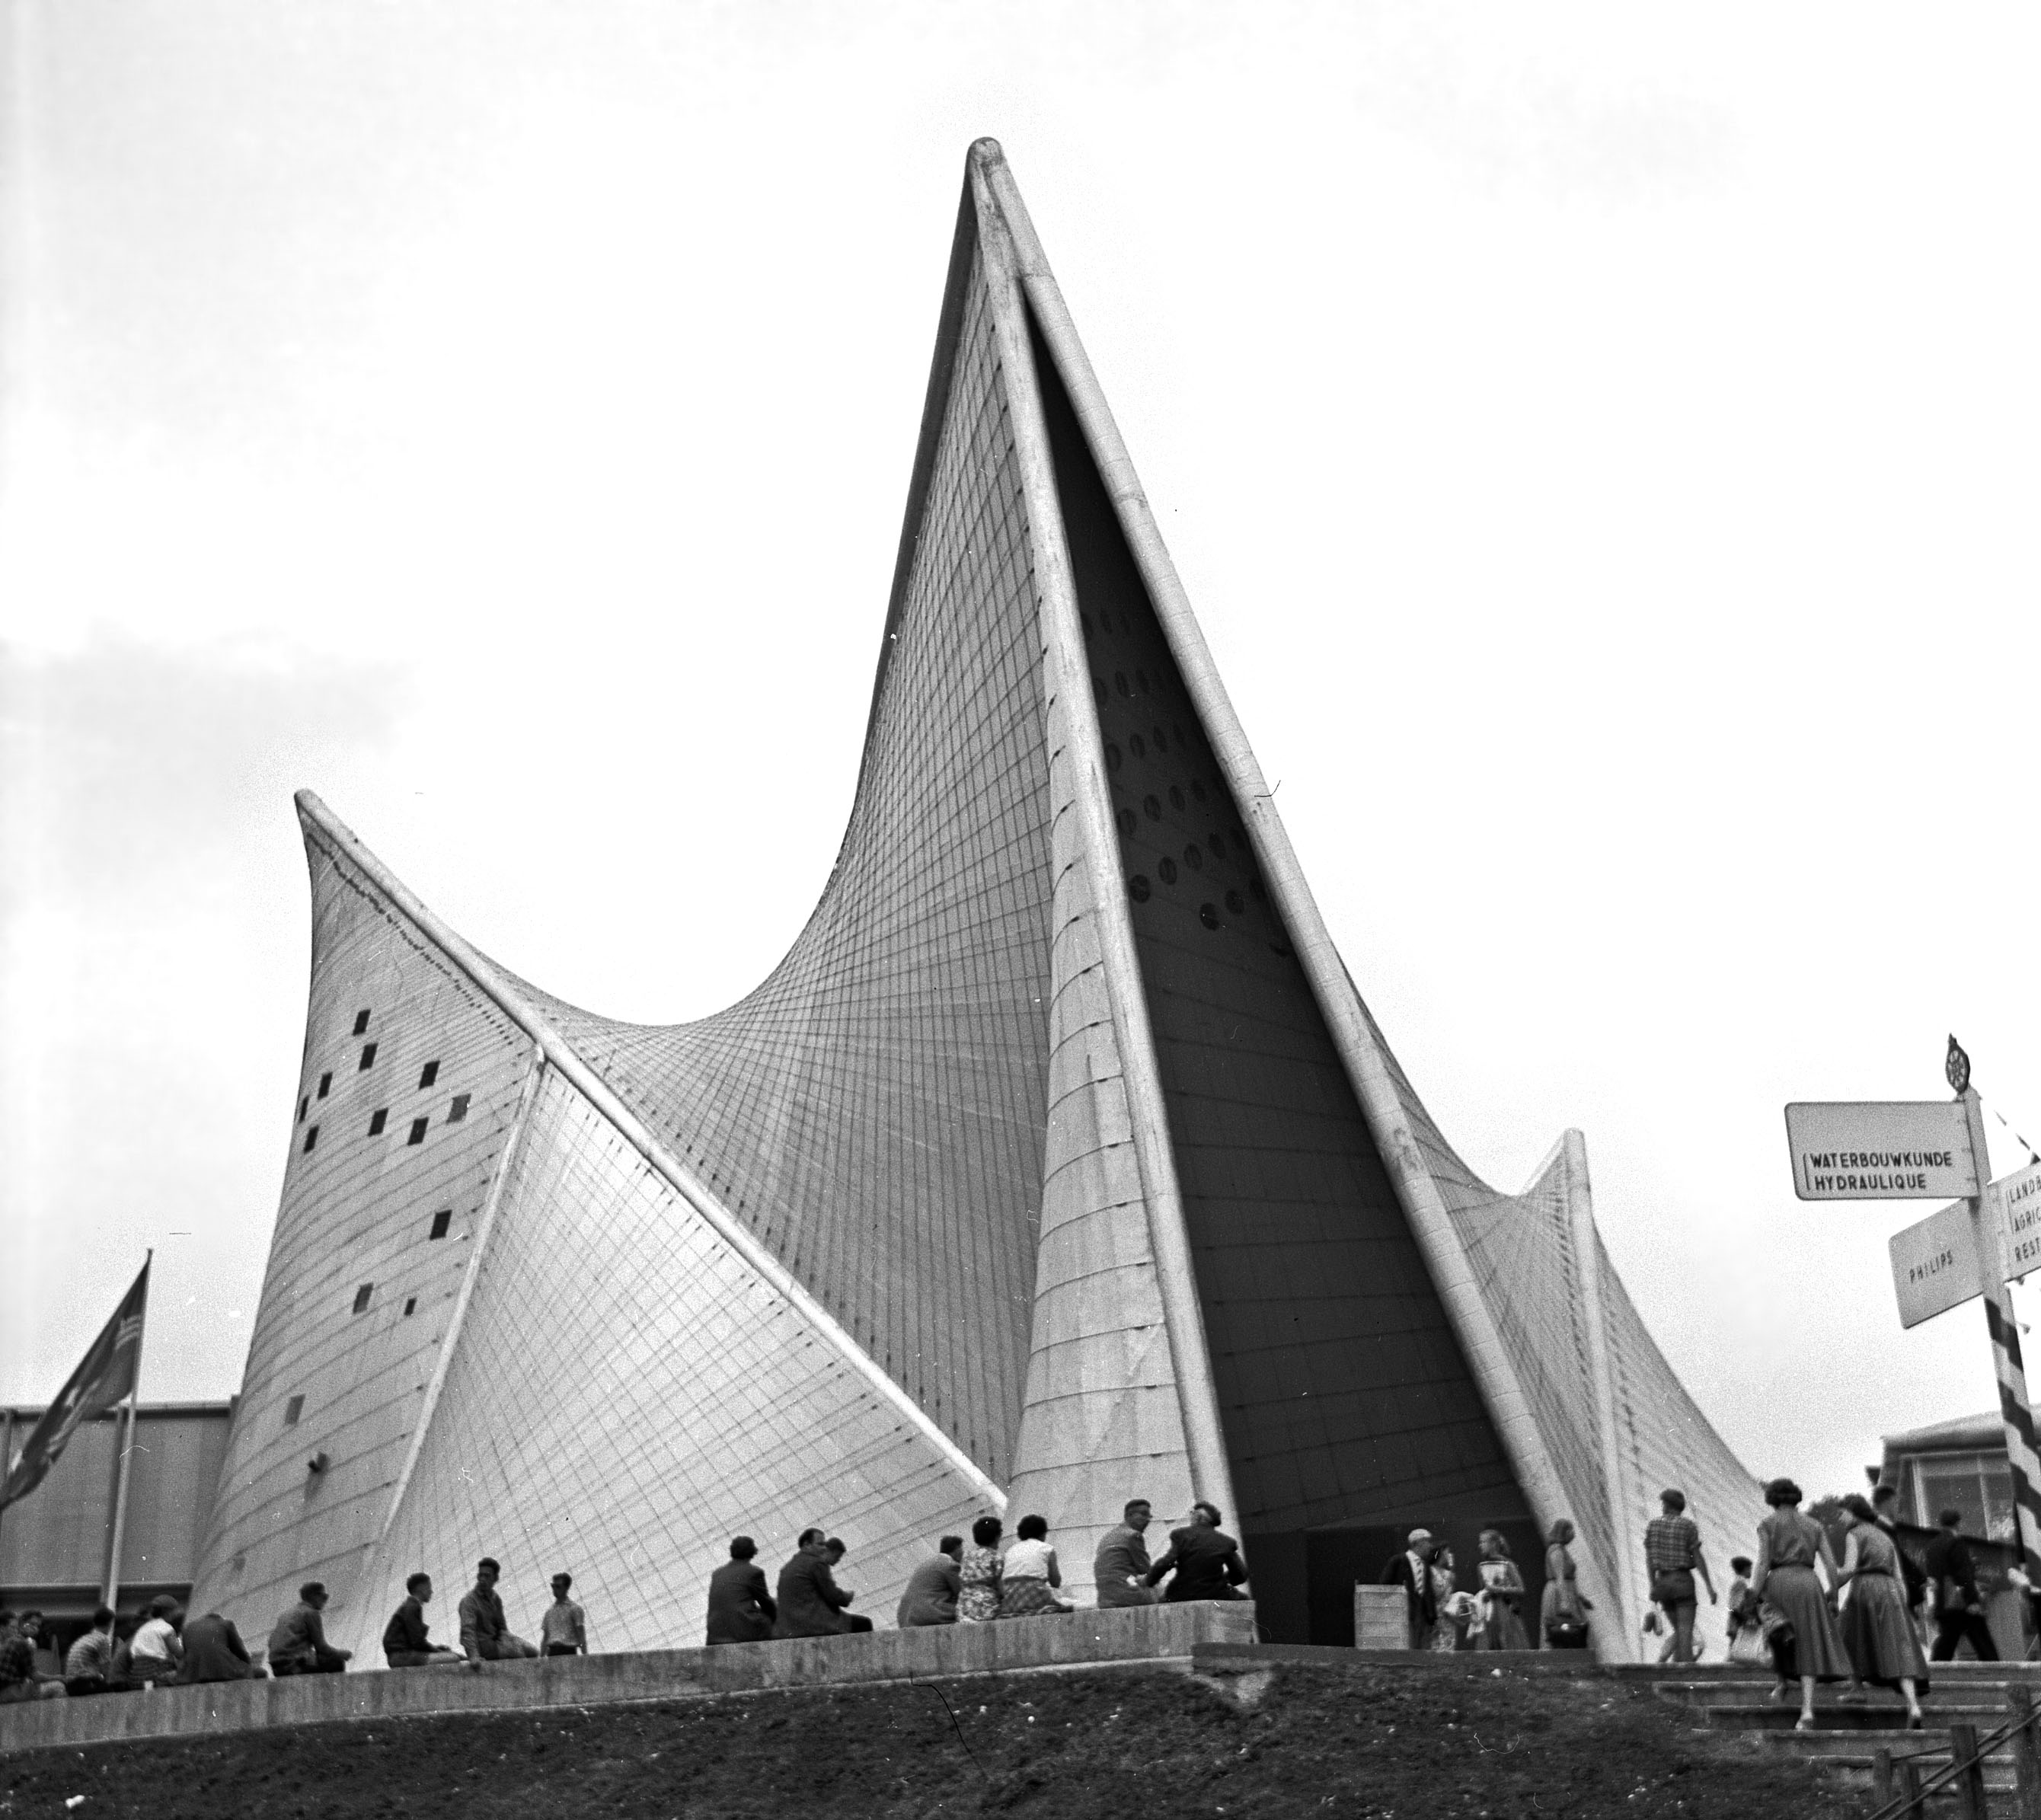
\includegraphics[width=0.5\textwidth]{img/expo58.jpg} 
%\captionsetup{justification=centering}
\caption{The Philips Pavilion \cite{wikipedia_2020_expo}}
\end{figure}

EXPO 70 in Osaka, Japan, also featured a number of groundbreaking spatial works. There, Xenakis presented a 12-channel tape composition titled \textit{Hibiki Hana Ma}, which translates to "Reverberation Flower Interval", was composed using the UPIC system. The UPIC\footnote{Unité Polyagogique Informatique CEMAMu (Centre d'Etudes de Mathématique et Automatique Musicales).} system was an instrument which allowed the composer to draw scores which would be interpreted by a machine\footnote{The software \href{https://www.iannix.org/en/whatisiannix/}{iannix} is the modern equivalent of the UPIC system.}. The graphical input device was used in conjunction with orchestral recordings, biwa\footnote{Japanese plucked instrument resembling a lute or guitar.} recordings, and snare drum recordings \cite{IannisXe73:online}. For the performance at the Japanese Steel Pavilion the sound system featured 800 speakers situated above, around, and even under the seats. At the same time, in the German Pavilion, Stockhausen, along with 20 soloists, were performing in a spherical auditorium featuring 55 speakers and six small balconies. The auditorium had an acoustically transparent grid which allowed sound to emanate from below the seating area which seated 600 people \cite{zvonar1999history}.

\begin{figure}[h]%force figure here, top, strict
\centering
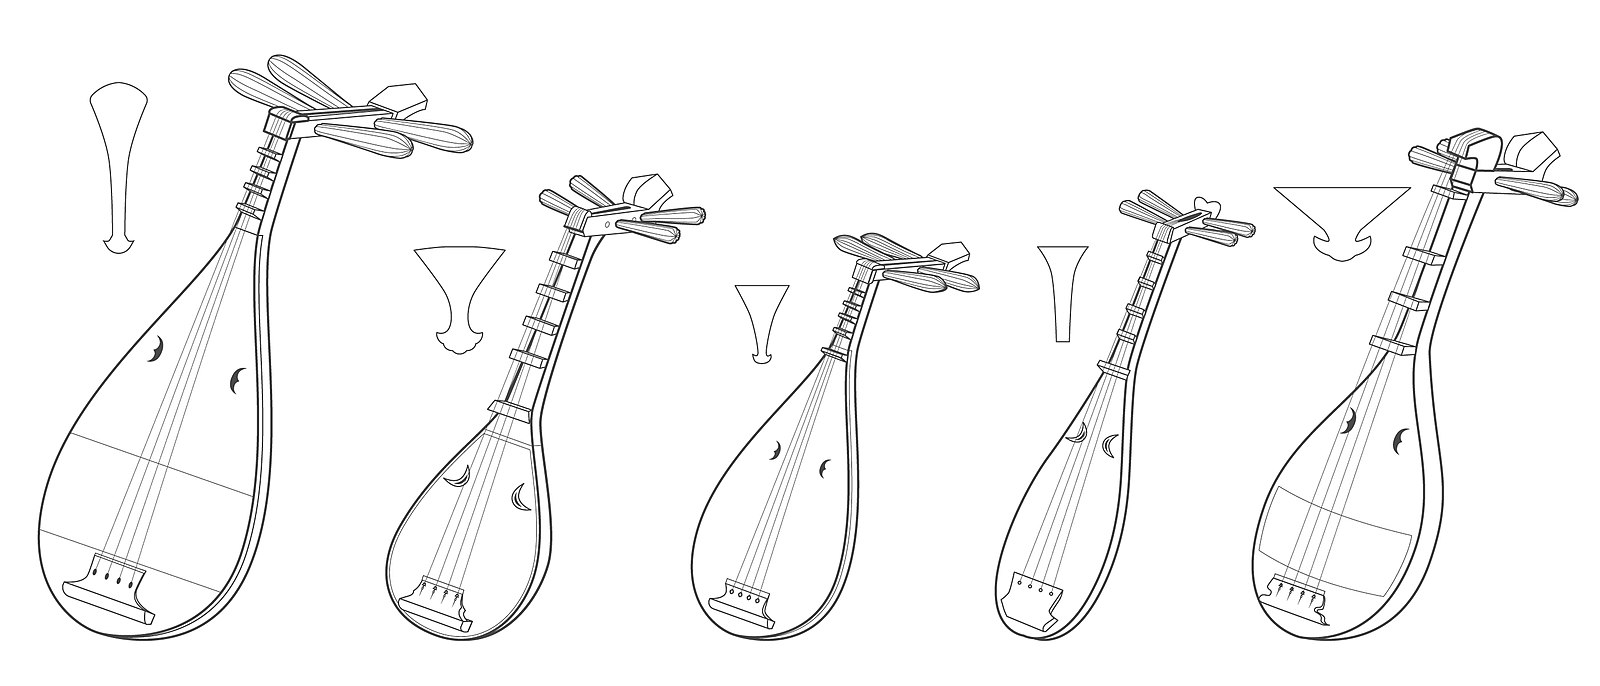
\includegraphics[width=0.7\textwidth]{img/types-of-biwa.jpg}
%\captionsetup{justification=centering}
\caption{Types of Biwa \cite{FileType46:online}}
%license: attribution share alike 4.0
\end{figure}

The Pepsi Cola Pavilion was another space created for EXPO 70 - this time designed by an American group called: "Experiments in Art and Technology" (EAT). The domes' 37 loudspeakers were arranged in a rhombus and could be driven with 16 monaural tape recorders and 16 microphone preamps for a total of 32 inputs. There were also 8 signal processing channels with amplitude modulation (AM), frequency modulation (FM) and various filters, which these sources could be routed to. Handsets were also distributed which could pick up sound in each of 11 zones. The dome was outfitted with laser beams and fog machines, and the walls of the dome itself were made of specular surfaces, for added dramatic effect. The dome was designed as a modular instrument, which could be reconfigured to fit the range of artists' visions \cite{bertrand2012pepsi}.

Given the wide range of creative options for spatialization of sound \cite{zvonar2000extremely} provides a list of the different types of electro-acoustic works in relation to their associated techniques - along with some influential composers representative of each method - to help us understand their differences:

\begin{enumerate}
    \item Live performance or "diffusion" of sound (Pierre Henry).
    \item Environmental multi-channel soundscape (John Cage).
    \item Classic studio multi-track tape composition (Karlheinz Stockhausen).
    \item Automated location control (Edgard Varèse).
\end{enumerate}

In this "live performance" setting, Pierre Henry created a repertoire of tape works which would be \textit{panned} around in real-time according to the desired trajectories manipulated by the composer. These works made use of Schaeffer's aforementioned \textit{Potentiometre d'espace} created in 1951, which translates to spatial potentiometer\footnote{A potentiometer is an electrical component which allows one to manually change the resistance between two points in a circuit.}. Henry also worked on diffusion works where stereo tapes would be played back over large loudspeaker systems. Examples of Cage's environmental works include \textit{HPSCHD}\footnote{Short for harpsichord. In collaboration with Lejaren Hiller, another American composer.}(1960) which used 58 channels - seven for harpischord soloists and 51 for computer generated tapes. The result of all this sound sources was a dense microtonal sound mass. There were also 80 slide projectors, seven film projectors, and a 340-foot circular screen. The piece was 5 hours in duration, however, participants were encouraged to enter and leave the environment as they desired. The final two classifications refer to works which are: "fixed" - suggesting that the trajectories of sounds are imprinted into the tapes and never controlled during the performance - and, those which use an algorithm\footnote{In Varèse's case the algorithm was imprinted on tape.} to manipulate the real-time diffusion\footnote{Diffusion in this context meaning panning of sound sources in space.} of sound sources. 

David Tudor was another member of John Cage's group who developed a series of installations of similar nature. \textit{Rainforest} (1968) is his best known work. In this installation work speakers are placed inside objects in order to activate their resonant modes. The sounds are consequently picked up using contact microphones, after they have been altered by the cavities of these objects. In Tudor's work, there were usually 4 to 8 speakers, but because of the additional resonant objects, the total speaker count was generally higher. Alvin Lucier, famous for the acoustic feedback composition: "I Am Sitting in a Room" (1969), explored a similar concept using the resonant modes of a room to create his piece. While not psycho-acoustic in nature, we can consider Lucier's piece a sort of architecturally spatial piece, dictated in large part by the geography and environment.

John Chowning, famous for his discovery of frequency modulation (FM), as a musical technique, at Stanford, also published and composed spatial pieces still relevant today. "The Simulation of Moving Sound Sources" \cite{chowning1971simulation}, published by Chowning in 1971, is considered a seminal piece of technical literature by a pioneering computer musician detailing his spatial audio algorithms. Chowning describes a system for the synthesis of spatial sound relying on FM and reverb to describe moving sources. FM in this context was used to simulate \textit{Doppler shift}. His piece \textit{Turenas} (1972), which makes use of a quadraphonic layout and this algorithm, was composed at CCRMA\footnote{Center for Computer Research in Music and Acoustics (CCRMA) at Stanford is an important computer music research facility.}, an important institution he was a founding member of. It should be noted here that the substantial difference in speaker count between \textit{Poème Électronique} and \textit{Turenas} had no impact on the historical importance of these works. It is easy to believe that higher speaker count is crucial for great spatial music - Chowning's work demonstrates that this is not always the case.

Part of the reason for the lower speaker count in some of these early works can be explained by the exorbitant cost of computers capable of handling these processes at the time. In 1981 at IRCAM\footnote{Institut de Recherche et Coordination Acoustique/Musique. Or, Institue for Research and Coordination Acoustical/Musical. It is organizationally linked to the Centre Pompidou in Paris.} the 4X synthesizer used to perform Pierre Boulez's\footnote{French composer perhaps best known for his large orchestral works featuring live electronics (26 March 1925 – 5 January 2016). Founding member of the aforementioned IRCAM.} \textit{Répons} (1985) had a cost of \$100,000. Today it is possible to recreate the synthesized elements of this piece using a personal computer \cite{zvonar2000extremely}. 

\begin{figure}[ht!]%force figure here, top, strict
\centering
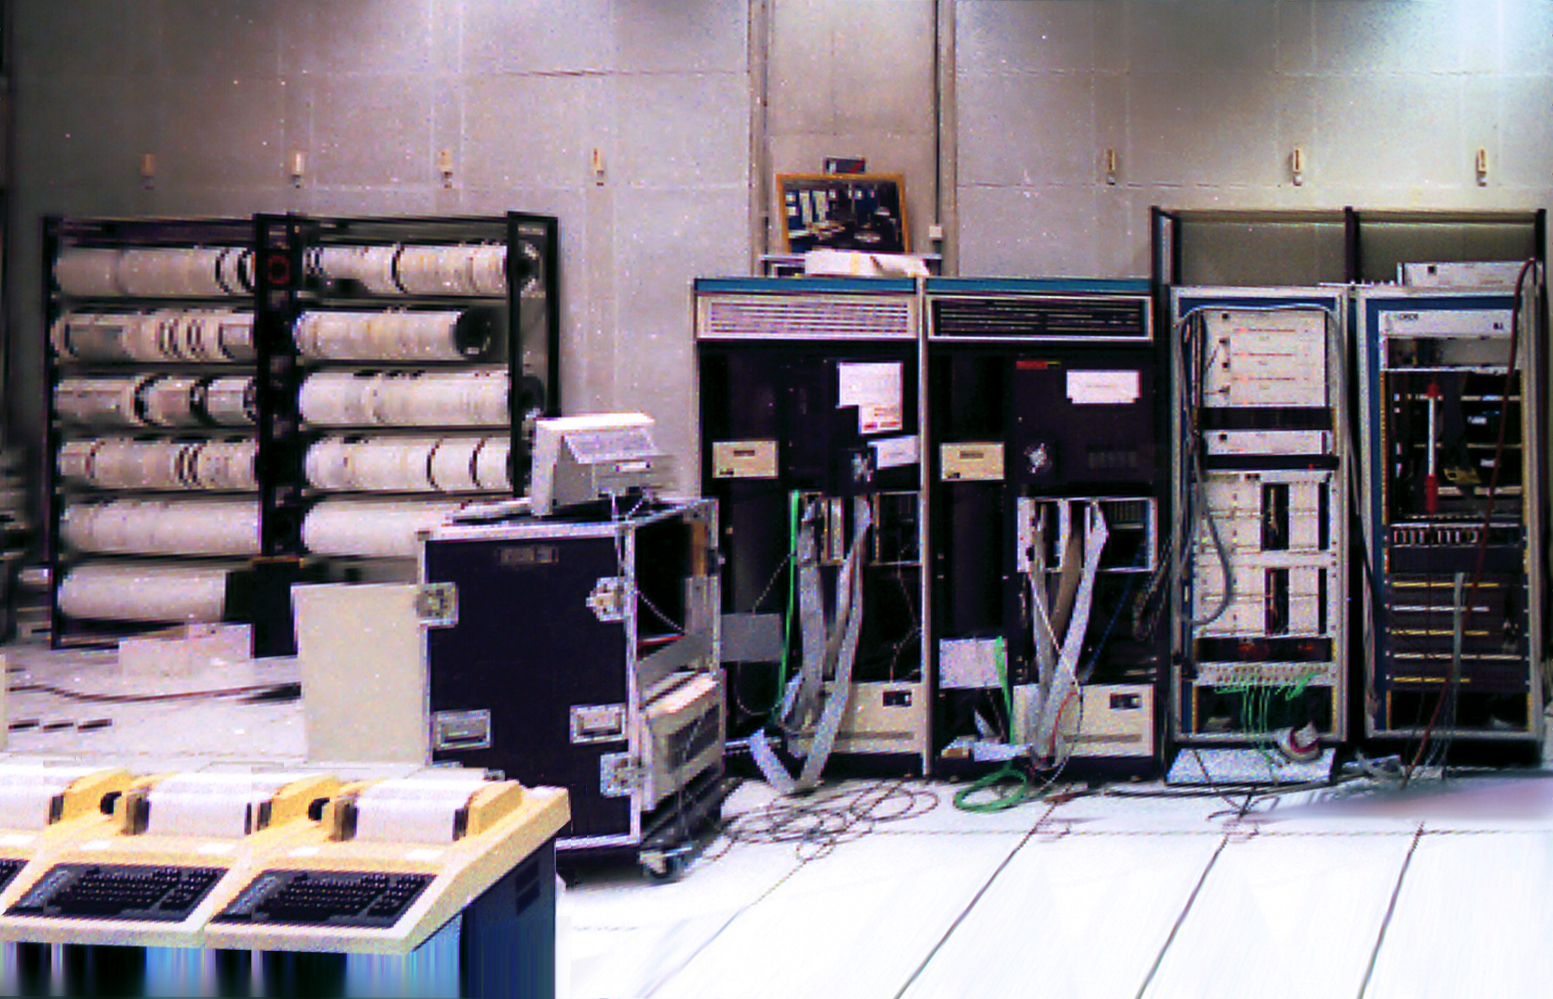
\includegraphics[width=0.7\textwidth]{img/ircam-4x.jpg} 
%\captionsetup{justification=centering}
\caption{IRCAM 4X \cite{FileIRCA45online}}
%  Creative Commons ShareAlike 1.0
\end{figure}

% \todo[inline]{Where can we find a patch for Repons? Is there a Pd port?}

Roger Reynolds in the 70s also created a number of important works. Reynolds used voice recordings in his \textit{Voicespace} pieces such as \textit{Still} (1975) and \textit{Eclipse (Voicespace III)} (1979). The pieces were created using analog equipment including: recorders, mixers, reverbs, and voltage controlled spatial location systems. \textit{The Palace (Voicespace IV)} (1980), used quadraphonic sound system and recording of singer Philip Larson, which were analyzed and processed to emphasize the harmonic content. A reverberation algorithm also gave the illusion of an impossibly huge space \cite{zvonar1999history}. Reynold's continued working with sound analysis in \textit{Transfigured Wind II} (1984). The piece features quadraphonic tape, solo flute and orchestra. There is also analysis and resynthesis of the flute using software created by IRCAM. \textit{Watershed IV} (1996), for solo percussion and computer is another example of his spatial works, this time featuring 6 speakers on stage and 2 additional surround speakers. The piece was performed by Steve Schick (1954), American percussionist and conductor. \textit{The Red Act Arias} (1997), another work by Reynolds, is based on the Greek tragedy of Clymenestra and Agamemnon. The piece features orchestra, chorus, and octophonic processed sounds using the \textsc{cmusic} "space" unit generator. \textsc{cmusic} was developed in 1980 by Richard Moore at the Computer Audio Research Laboratory (CARL) of the Center for Music Experiment at the University of California at San Diego (UCSD) \cite{moore1982computer}. \textit{Justice} (2000), by Reynolds, featured soprano, actress, percussionist, tape and computer spatialization. 

In Montreal in 1999, ACREQ\footnote{\href{https://www.thecanadianencyclopedia.ca/en/article/acreq-emc}{Association pour la Création et la Recherche Electroacoustiques du Québec}. The first non university-affiliated organization in Canada exclusively dedicated to electro-acoustic music.} reproduced Pierre Henry's \textit{L'Apocalypse de Jean} (1968) through a 24.6 sound system using the commercial CD as the sound source. Henry is one of the pioneers of this \textit{diffusion} practice, in which mono or stereo signals are played back over a multitude of speakers. Sound systems such as the ones proposed by Henry are sometimes referred to as an \textit{acousmonia}\footnote{Acousmonium being the singular.}. Here the sound system becomes and instrument itself, to be performed by the composer using, traditionally, musique concrète. François Bayle designed the first acousmonium in 1974 which was used by Groupe de Recherches Musicales (GRM)\footnote{Institute created by Pierre Schaeffer in 1958 in France.}. The Gmebaphone and Cybernéphone at the Institut International de Musique Eléctroacoustique de Bourges (IMEB)\footnote{Central France.}, and the Birmingham\footnote{Second largest city in England.} ElectroAcoustic Sound Theatre (BEAST) are a few other examples. Notable American acousmonia include composer Stan Shaff's \textit{Audium: A Theatre of Sound-Sculpted Space} and the Recombinant Media Lab both in San Francisco. These are all historical examples of multi-channel sound systems, since then several institutions have developed their own diffusion systems for spatial music performance. These historically relevant systems have also evolved over the years from diffusion systems to arrays supporting modern spatialization algorithms.

\begin{figure}[ht!]%force figure here, top, strict
\centering
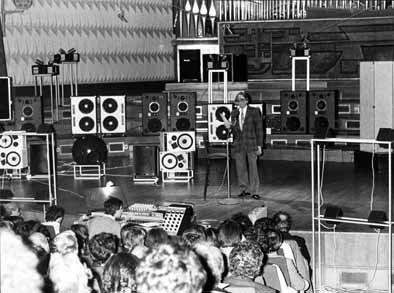
\includegraphics[width=0.7\textwidth]{img/acousmonium.jpg} 
%\captionsetup{justification=centering}
\caption{Pierre Schaeffer Presenting the Acousmonium \cite{FilePsco51online}}
% This file is licensed under the Creative Commons Attribution-Share Alike 3.0 Unported license.
\end{figure}

Denis Smalley is another pioneering composer who has worked, and continues to work, extensively with space in his acousmatic compositions. Smalley has created his own language to describe sound which he describes as spectromorphological. Has Smalley puts it in \cite{smalley1997spectromorphology}:

\begin{quote}
    Spectromorphology is not a compositional theory or method, but a descriptive tool based on aural perception. [...] Although spectromorphology is not a compositional theory, it can influence compositional methods since once the composer becomes conscious of concepts and words to diagnose and describe, then compositional thinking can be influenced, as I am sure my own composing has been.
\end{quote}

Smalley has created an extensive dictionary to describe the way he envisions and articulates his music. \cite{blackburn2011visual} pictorialized some of these concepts in order to help the reader better understand Smalley's language. Here we will only present written definitions of some of the most popular concepts defined by Smalley. 

\begin{enumerate}
    \item \textbf{Source-bonded space:} refers to the spatial zones and mental images produced by, or inferred from, sounding sources, and their causes (if there are any). 
    \item \textbf{Source bonding:} related to source-bonded space, is the \textit{natural} tendency to relate sounds to \textit{supposed} sources and causes, and to relate sounds to each other because they appear to have shared or associate origins.
    \item \textbf{Perspectival space:}  relating to our perspective, can be further sub-divided into various perspectives.
    \begin{enumerate}
        \item \textbf{Prospective space:} frontal image, which extends to create panoramic space.
        \item \textbf{Panoramic space:} the breadth of the prospective space, extending the limits of the listener's peripheral view.
        \item \textbf{Circumspace:} the extension of prospective/panoramic space so that sound can move around, above and through the space occupied by the listener.
    \end{enumerate}
    \item \textbf{Spectral spatiality:} impression of space and spaciousness evoked by occupancy and motion within the range of audible frequencies.
\end{enumerate}

This list forms only a small part of the language created by Smalley to describe his music. \textit{Pentes} (1974), \textit{Empty Vessels} (1997), \textit{Wind Chimes} (1987) and \textit{Valley Flow} (1991–92), are a few of Smalley's most notorious compositions in which he attempts to sonically articulate all these different concepts. \cite{o2011soundscape} provides a closer examination of these works. According to O'Callaghan, many of Smalley's works utilize mimetic properties. In other words, the sound design aims to simulate real world sounds using electro-acoustic means. Much like work done by Barry Truax such as \textit{Riverrun} (1986) which utilizes granular synthesis to emulate the sound of a flowing river.

This brings us to the conclusion look into the history of spatial music. As we can see, while many contemporary composers might attribute the development of spatial music to composers of the 20th century, the use of spatial elements in composition has a longstanding tradition that spans hundreds of years. 

\todo[inline]{ macedo-2015-snd-in-space.pdf} 

\section{Installation works}

In this section we wish to enumerate some of the \textit{sound artists} whom have created interesting and powerful spatial music works in their practices. In contrast to concert events, these installation pieces are designed to be shown in art galleries and experienced by hundreds of people over many days. 

Michael Asher (July 15, 1943 – October 15, 2012), the first in our list, was a conceptual artist who worked with sound absorption and acoustic phase cancellation in his works. In \textit{Spaces} (1969), Asher created a sonic space which resulted in different aural experiences as one walked around the gallery. Michael Brewster also worked with these ideas as well as: room resonances, standing waves, and acoustic shadows. Both of these artists sought to manipulate air as a sculptural medium. Some of Brewster's most famous works include \textit{allAROUNDyou} (1998), \textit{See Hear Now} (2001) and \textit{full o’stuff} (2000) \cite{macedo2015investigating}. 

Maryamme Amacher is one of the most ambitious and well-known artists of sound art employing spatial elements. Her work explored structural vibrations and structure-borne sound. In \textit{Music for Sound-Joined Rooms} (1980) she transformed an old house into a resonator by placing powerful speakers inside it. In \textit{City Links} (1967-80) she installed microphones at the Buffalo Airport and Boston Harbour and connected the spaces sonically with speakers. Listeners in Buffalo heard the sound of the Harbour, while people in Boston heard the sounds of the airport. Amacher also created CDs with music specifically meant for loudspeaker reproduction. She believed the physical characteristics of the listeners space was instrumental in appreciating her work\cite{ouzounian2008sound}. Amacher is also known for exploring sonic relationships with \textit{otoacoustic emission} in her work. Otoacoustic emission refers to sound that originate from the inner ear, in some people it manifests as a medical nuisance called \textit{tinnitus} \cite{brummer2017composition}.  

Edwin van der Heide, a Dutch sound artist, also explored architectural interactions with sound in \textit{Speed of Sound} (2007). The piece explores the effects of four corridors in the shape of rings on sound. As Heide puts it in \cite{TheSpeed60online}:

\begin{quote}
    "The propagation of sound in the rings of the water reservoir of Prenzlauerberg in Berlin is the starting point for the installation. The acoustic sound in the space is being picked up, transformed and re-entered in the space. The transformations, delays and spatial interconnections are part of a time based process that can be seen as a composition for the environment."
\end{quote}

Similarly, in \textit{Crescents} (2010) Raviv Ganchrow explores the reverberance and general acoustic character of spherical domes in Estonia. In this example the acoustic space is central to the work, and the variability from moment to moment is created by the dynamic architectural features. However, there are also sound artists who have explored spatialization in their works. 

In two of his \textit{Three Sounds} (1971) Howard Jones explored the motion of sound \cite{macedo2015investigating}. In \textit{Linear Relay} a metronome sound is played through 20 speakers all aligned in different ways. \textit{Area Relay} also explores this idea by using 9 speakers assembled in a grid playing different sounds to provide the illusion of distance and depth. Bernard Leitner's installation \textit{Sound Space} (Berlin, 1984) used 48 speakers hidden behind panels in the walls of a staircase to simulate trajectories.  

\textit{Sound Island} (1994) by Bill Fontana, an American sound artist, used 48 speakers across the Arc de Triomphe in the centre of Paris to receive and reproduce sounds from the coast of Normandy. There is also Max Eastley's \textit{Sutton Edge} (1991) in which Max installed a set of ad hoc wind harps in an open site \cite{ray2006soundscapes}. William Louis Sorensen explored a similar idea in \textit{Landing Ground for Waders} (1983) using more humble materials such as wine bottles, wood and plastic. 

Two other related examples are Westerkamp's \textit{soundwalks}, in which listeners are simply asked to traverse any environment with the main purpose of listening, and Steve Peters’s \textit{Here-ings} which are collections of recordings in central Mexico, meant to transport the listener to the space\footnote{https://www.spsoundart.com/hereings}. 

A final sound art work we sought to include is Alvin Curran's 1987 \textit{Notes from the Underground}. The work was part of a larger collection titled Music from the Center of the Earth, however the rest of the remaining works never seem to have been realized, they only exist in concept. In \textit{Notes from the Underground} the idea was to create sound walls by physically burying speakers underground. Its realization was commissioned by the Ars Electronica Festival\footnote{A prestigious media arts festival in Lintz, Austria.} in 1991. The collaborator in the project, Mellisa Gould, used the floor plans of an old Berlin synagogue for this Holocaust memorial. The music was composed a Mills College's Center for Contemporary Music, in Oakland, California. Then the tapes were used to drive 72 speakers in groups of 8 attached to 9 stereo amplifiers\cite{curran1994music}\footnote{The system was designed by Tom Erbe who studied at Mill's College at the time.}

\todo[inline]{xenakis "polytopes"}
% https://www.theguardian.com/music/tomserviceblog/2013/apr/23/contemporary-music-guide-xenakis

\section{Contemporary Spatial Music} \label{sec:contemp_works}

Several authors have explored the use of space in composition with varying degrees of success. In this section we will explore the techniques and aesthetics employed by these composers. The following pieces in this section were selected because the composers all use "spatial articulation as a central element in the musical construction\footnote{Lyon in Sound Anthology Program Notes CMJ 41:1}". Our hope is that by understanding the methods and processes used by some of these composers the reader might be better equipped to create impactful spatial music and carve their own style to differentiate themselves from the many other artists in this field. 

\subsection{Concert music}

\cite{hagan2017sound} offers an overview of some of the current leading figures in the development of spatial music. Before diving into the particular composers and their works two noteworthy facts stand out from these program notes. The first interesting information is that the delivery of the musical material\footnote{Found \href{https://muse.jhu.edu/article/656037}{here}. Jump to end of page to download audio files.} for public consumption used a stereo format with binaural properties. What this means is that the music does have spatial attributes, but much of it will be lost because the listener will not have the ability to rotate the soundfield in relation to their head orientation. The second noteworthy piece of information is that in this anthology Hagan and Lopez-Lezcano opted for \textit{static binaural synthesis} while the rest create binaural recordings - using a dummy head. This offers the listener the possibility, albeit with different materials, to experience the quality changes between both spatial audio rendering methods.

We will discuss the different composers in order of appearance within the program notes. \textit{Spin} (2016) by Ludger Brümmer was created by taking video files and converting these into noisy sound material. The sound is then organized contrapuntally and the resulting soundfield is spun over the course of the piece. This piece was recorded at the \href{https://zkm.de/en}{ZKM Klangdom} in Germany using 32 channels. \cite{ramakrishnan2006zkm} provides a rich description of the "Kubus" which is the name of the concert hall where this piece was recorded. \textit{Spin} has a very synthetic quality to it and resembles the score someone might hear in a sci-fi film. It features noises one could qualify as other-wordly: warps, glitches and combed filters appear to be prominent. Ludger's former interests also include physical modeling and granular synthesis, both of which also appear to be exemplified here. 

\begin{figure}[ht!]%force figure here, top, strict
\centering
\includegraphics[width=0.7\textwidth]{img/zkm-commons.jpg} 
%\captionsetup{justification=centering}
\caption{ZKM - wikimedia commons}
\end{figure}

\textit{Sveti Kliment} (2007) by Robert Sazdov and was recorded at the Sonic Lab of the Sonic Arts Research Centre (SARC) in Belfast, Northern Ireland. The composition was inspired by Saint Clement of Ohrid from the Orthodox Church of Macedonia, a patron saint of education and language who committed his life to: research, teaching, and improving the lives of "those in his diocese". The piece open with the natural sound of a flute but quickly morphs into a soundscape of reversed noises and unintelligible speech snippets. The timbre of the flute reappears as a thematic motif and its reverberation is frozen and played over, using the same instrument. The timbre of the flute seems to be that of a ethnic instrument perhaps in reference to the Balkans. 

\cite{lynch2017perceptual}, co-authored by Sazdov, discusses some of the most popular and powerful spatialization techniques, used routinely by composers. In this paper, the author used four of these critical techniques in a subjective experiment in order to determine listener preferences. The techniques used in that experiment are described as follows:

\begin{itemize}
    \item \textbf{Timbre spatialization}: in this technique the source signal is copied and routed to multiple band-pass filters. These filtered versions of the original sound signal are sent to various speakers. The bandwidth of these filters can be modulated for artistic effect. 
    \item \textbf{Spectral splitting}: is a technique used in periphonic configurations, wherein the loudspeakers in the upper regions are assigned a high pass-filter in order to cut frequencies below a certain range. 
    \item \textbf{Amplitude point-source panning}: amplitude point-source panning consists of placing monophonic sound signals on individual loudspeakers. Perceived movement of sounds between loudspeakers is achieved by changing amplitude levels of individual speakers.
    \item \textbf{Dynamic spectral subband decorrelation}: similar to timbre spatialization but with modulated center frequency for band-pass filters and added decorrelation copy (at same speaker) created using modulating sample delays. 
\end{itemize}

In addition to these four common techniques, Sazdov lists authors who have experimented with granulation approaches to spatialization. More recently \cite{rossetti2020studying}, Rossetti proposed a HOA \textit{granular synthesis} system in which individual grains are spatialized using 7th order ambisonics. Curtis Roads, famous for his use of granular synthesis (GS) in composition describes granular synthesis as:

\begin{quote}
    "a kind of synthesis based on grains, a microacoustic event with a duration near the threshold of human auditory perception normally presenting a duration between 20 and 400 msec. The grains, by definition, capture two perceptual dimensions: the time-domain and the frequency-domain information, and each grain has a waveform shaped by an amplitude envelope. The GS is an automation process in which thousands of grains are combined over time, creating sound textures (clouds or masses) of different densities and frequency ranges." \cite{roads2004microsound} 
\end{quote}

Another related approach undertaken by Einbond \cite{einbond2017mapping} involves using descriptors of sound samples to dictate the spatialization. This approach involves two stages: analysis and re-synthesis. In the analysis stage, sound grains are created and organized in Euclidean space using analysis processes such as: Mel Frequency Cepstrum Coefficients (MFCC)\footnote{An explanation of MFCC is outside the scope of this text, we refer the reader to \cite{terasawa2005perceptual}.}, for example. These grains can then be played back using concatenative synthesis and spatially distributed based on their Euclidean coordinates. In the Pd environment we recommend using William Brent's \cite{brent2010timbre} toolbox for timbre analysis. 

\textit{Morphons and Bions} (2011) by Kerry Hagan is a real-time Puredata composition which relies on noise synthesis and randomness. \cite{hagan2012aesthetic} provides a richer description of the work. As opposed to Sazdov's piece, all the sounds in this piece are synthesized in real-time. According to Hagan: 

\begin{quote}
    "Because the work is built on a substrate entirely made of noise, the piece is situated within certain philosophical and aesthetic issues surrounding noise, its use, and its definition."
\end{quote}

Indeed, a lot of discussion has gone into the role of noise in contemporary music. Despite the abundance of noise in \textit{Morphons and Bions}, Hagan does not consider the piece to fall under the category of "noise music", given the harmonic and quasiharmonic patterns that emerge from the organization of sounds. One interesting ontological point raised by Hagan is the idea of noise being the main source of information in this work. This goes against established notions of engineers seeking to remove noise from signals. As she says: "the noise \textit{is} the signal". 

\cite{hagan2017textural} provides more technical information on the piece. Here, Hagan describes the two main synthesis method employed by this work, which were later combined into one. The first she describes as additive synthesis modulated with white noise which results in the following equation:

$$
x(t)=\sum_{k=1}^{6} w(t) \sin \left(2 \pi h(t) f_{0}(t) t+D(t) n(t)\right)
$$
where \\
$n(t)=$ white noise, \\
$D(t)=$ depth (amplitude of white noise) changing in time, \\ 
$f_{0}(t)=$ fundamental frequency changing in time, \\
$k=$ partial number, \\
$w(t)=$ Gaussian random variable with mean $1 / k$, and \\
$h(t)=$ Gaussian random variable with mean $k$.\\

As you can see the equation shows both AM and FM with noise as the modulating signal. Hagan also describes the use of band-pass filters with aleatory properties to further articulate her sounds. Hagan has adopted the terms "textural composition" to describe her music. Her work in this domain draws from the philosophical frameworks of Russolo, Cage, and Xenakis, and is driven by statistical methods, such a Gaussian distributions. \href{http://www.kerrylhagan.net/#m&b}{Her site} contains all the associated patches required to perform the piece live. Given the aleatory nature of the work, each rendition should be subtly different.

\todo[inline]{Hagan has other interesting spatial works we can talk about. Cubic Zirkonia}

\textit{Il Prete Rosso} (2013) Charles Nichols is a work for amplified violin, motion sensor and computer, written for Sarah Plum. The piece was inspired by Antonio Vivaldi, teacher and violin virtuoso, and translates to "The Red Priest" - nickname given to Vivaldi for his red hair and ordinance. In the piece the violin is looped live and played over while recorded elements are spatialized. The computer musician interjects with a wah filter, phaser and delay effects. The motion sensor, attached to the violin player is used to control the center frequency of the wah filter. The work was premiered at the Cube of the Moss Arts Center at Virgia Tech which yields an impressive 124.4 channel system.

The fifth artist in the anthology \cite{hagan2017sound} is Natasha Barrett. Her piece \textit{He Slowly Fell, and Transformed into the Terrain} (2016) in sixth-order Ambisonics uses IRCAM's Spat software. This piece is the longest from the collection lasting over 20 minutes. The composer applies HOA granular synthesis, a technique in which sounds are fragmented into thousands of smaller units for re-synthesis, applied to sound field recordings captured using a FOA commercial microphone. An interesting aspect of the work, not mentioned in the text, is the concept of privacy. Audio recordings taken in public are problematic as source material. Certain laws exist prohibiting artists to use these materials without permission. Through the use of granular synthesis, the material quality of voices is maintained, but the dialogue because unintelligible, making this a non-issue. \cite{barrett2016musical} also references the HOA granular synthesis unit developed at IRCAM. The system, titled \textit{Grandad} encodes each individual grain of sound in 9th-order ambisonic and can be heard in the second movement of \textit{Hidden Values} (2012), also by Barrett. 

\todo[inline]{Barrett has other papers that talk about her ambisonic pieces. We should add them to this paragraph.}

\textit{Space, S[acred|ecular]} (2015) was written by Fernando Lopez-Lezcano using impulse responses capture at Hagia Sophia: a cathedral turned mosque turned museum, featuring a reverberation time of over ten second\footnote{Depending on where the impulse response is taken.}. The building in Istanbul, Turkey, was acoustically sampled in order to recreate its sound using a new reverb technique for Higher Order Ambisonics (HOA). Fernando's use of two instruments, voice and percussion, alludes to the dual nature of the religious space.  \cite{lopez2014architecture} describes the reverb method, which consists of using an intermediary decoder for the convolution reverb. This means that the HOA reverb can be implemented even if the playback system does not support HOA. The impulse responses were processed from balloon pops using an analysis/re-synthesis method which measures echo density and energy at multiple frequency bands. The technique was informally compared in a listening test with the favoured sine swept technique to good effect \cite{abel2010estimating}. The entire piece was written in \href{https://ccrma.stanford.edu/software/snd/snd/s7.html#juce}{s7}, "a Scheme implementation [of Common Lisp Music] intended as an extension language for other applications\footnote{Scheme is a programming language which is part of the Lisp family. Lisp is one of the oldest low-level programming languages (only Fortran is older by one year).}". The mixing process, as well as the reverb, were all implemented using open source software. This included the binaural decoding which suggests that, in theory, no HDLA is needed for creating music for these systems. 

\todo[inline]{FLL might also have more works we want to add. We also need to find a citation for the image from Hagia Sofia.}

\begin{figure}[ht!]%force figure here, top, strict
\centering
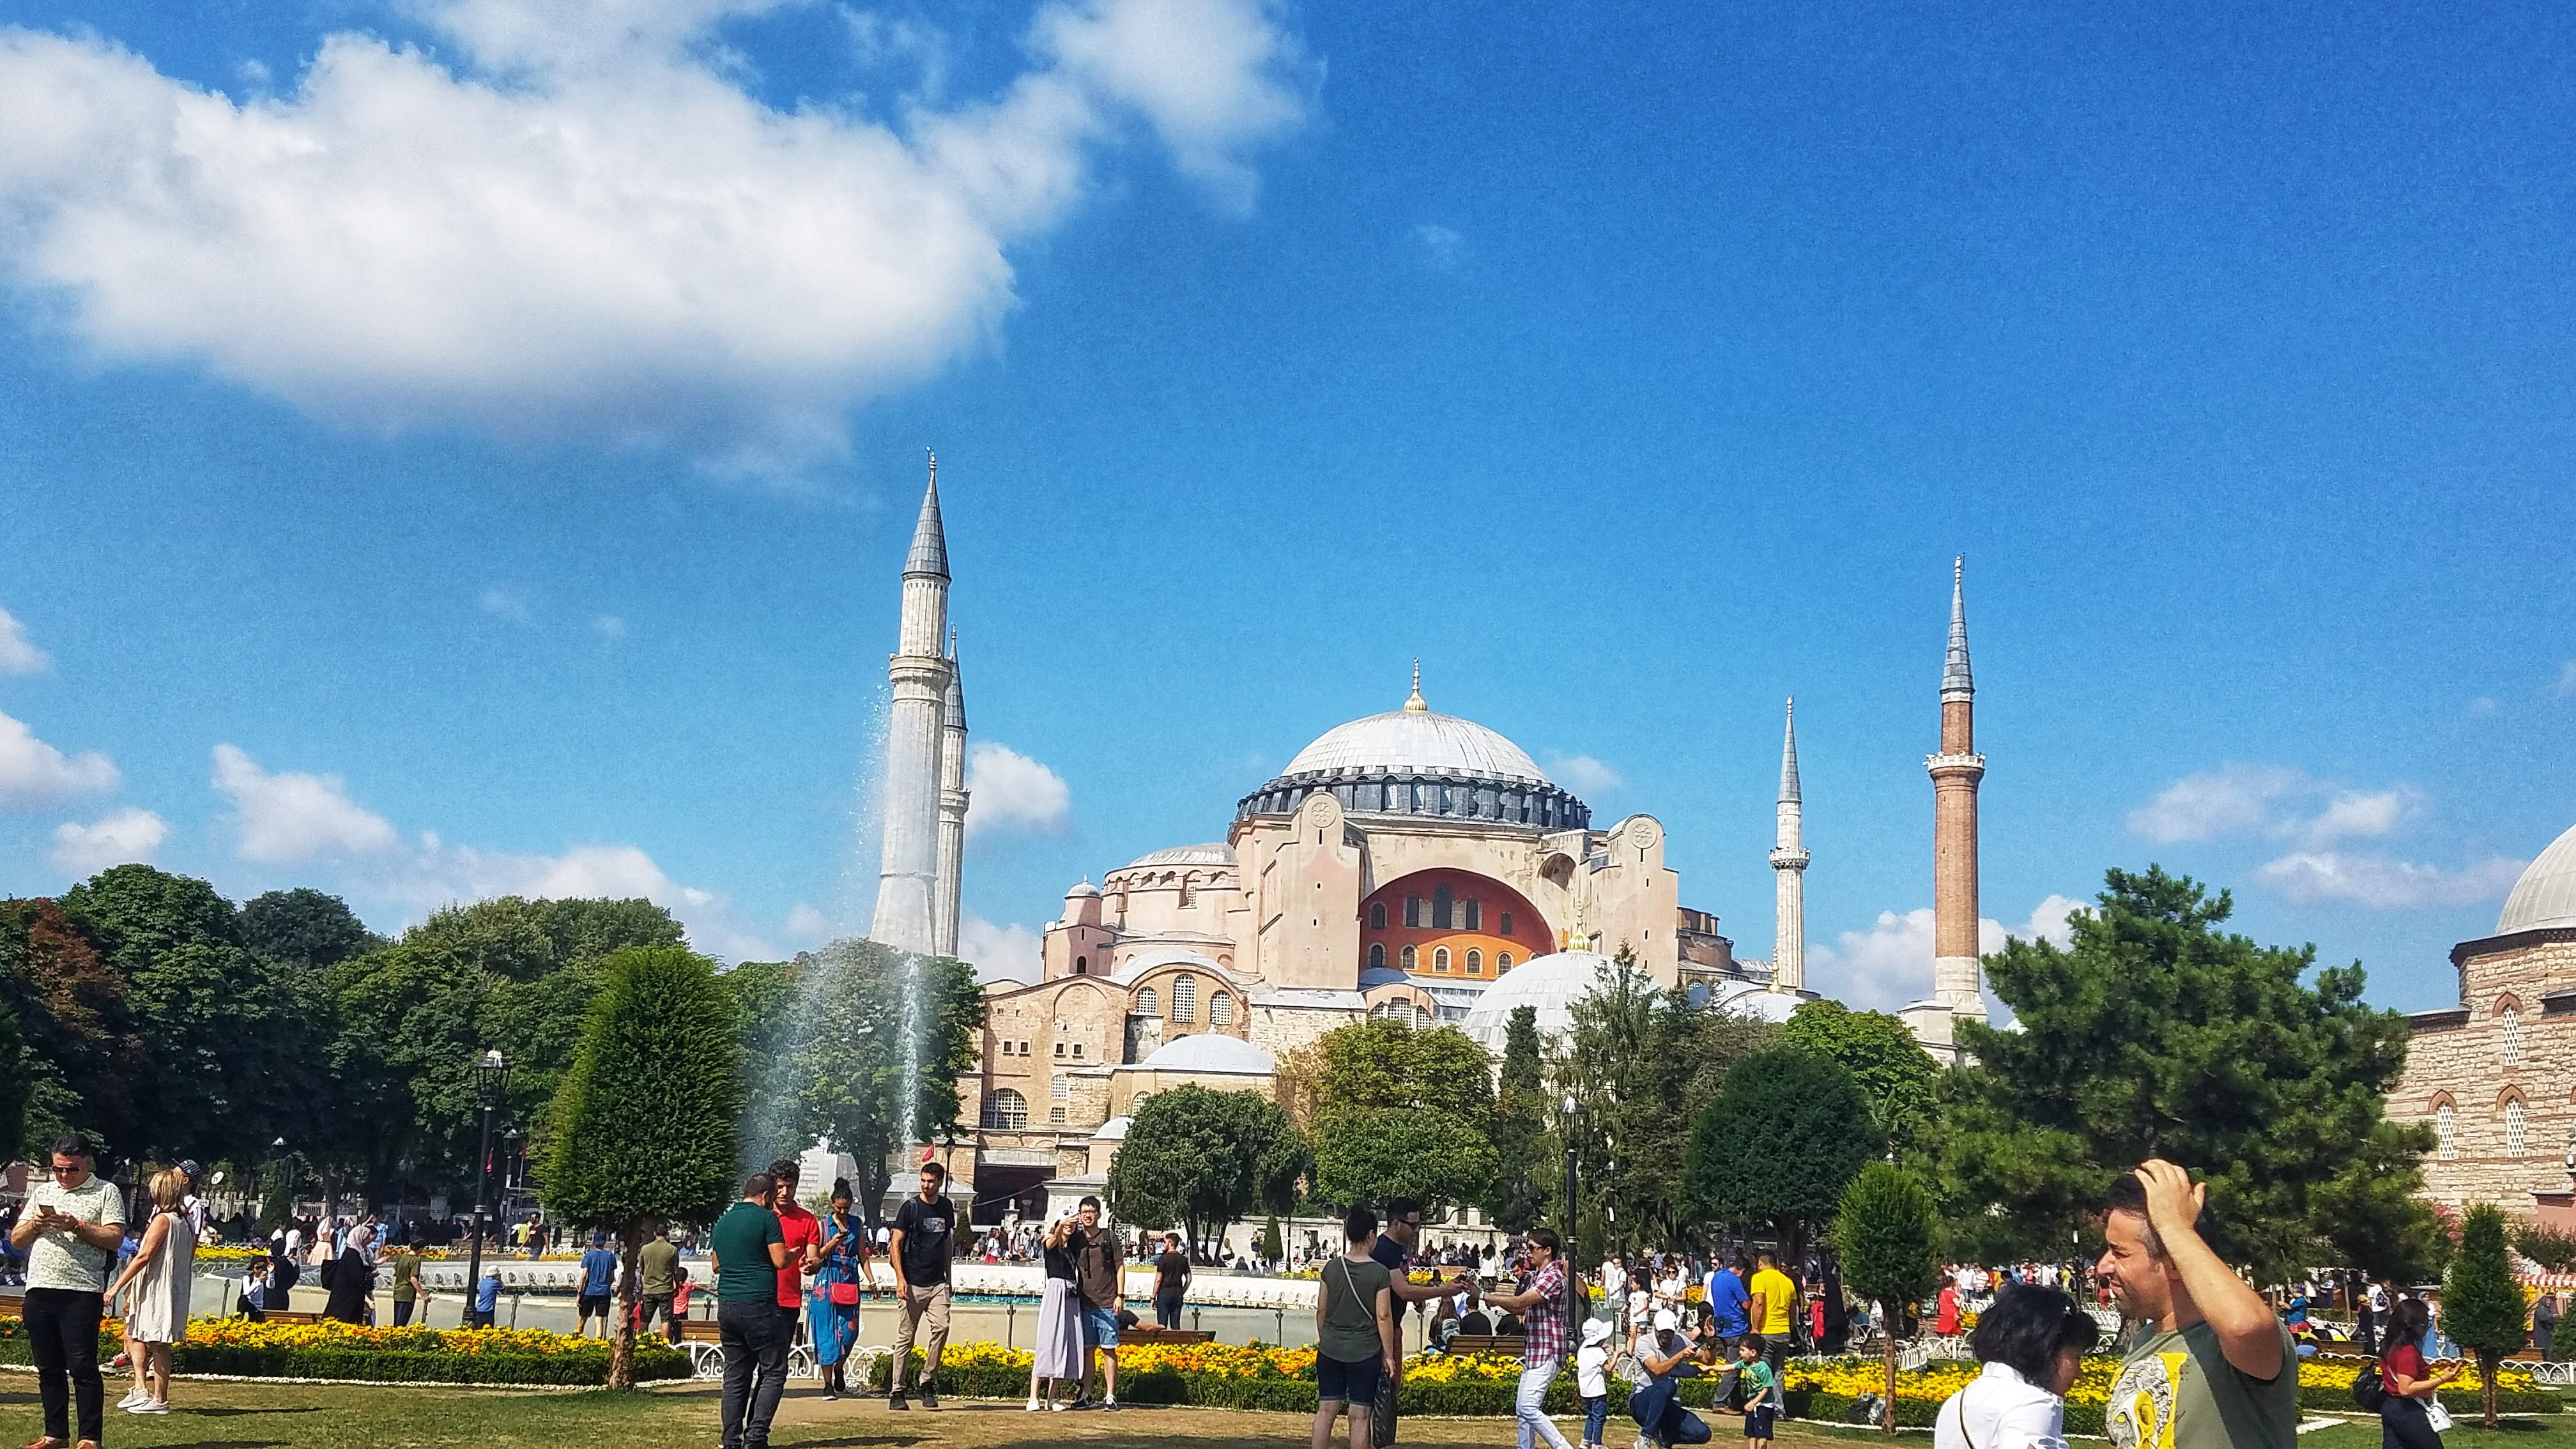
\includegraphics[width=0.7\textwidth]{img/hagia-sofia.jpg} 
%\captionsetup{justification=centering}
\caption{Hagia Sofia - wikimedia commons}
\end{figure}

The final piece included in the anthology \cite{hagan2017sound} comes from Gerriet K. Sharma and is titled \textit{mirage 4} (2015). The piece was composed with and for the icosahedral\footnote{Speaker approximating a sphere with 20 faces and one speaker for each phase of the geometry.} loudspeaker developed by the Institute of Electronic Music and Acoustics (IEM) at the aforementioned ZKM\footnote{ZKM stands for "Zentrum für Kunst und Medien" which translates to "Center for Art and Media Karlsruhe", Karlsruhe the city in Germany where the cultural center is located.}. This icosahedral speaker, takes the concept of ambisonic microphones, which capture soundfields at a single point, and invert the mechanism, attempting to project a soundfield from a single point in space, with increasing resolution based on the number of transducers. 

\cite{wendt2017perception} by Wendt, Sharma, et al. discusses the ability of such a system to reproduce accurate spatial dimensions of sound for compositional means. The system is indeed capable of creating the impression of moving trajectories of sound by exploiting wall reflections which are perceived as virtual sources. These coincident speaker arrays can be considered as a portable and affordable means for spatial music reproduction. The greatest benefit these provide, for composers, is the ability to reproduce \textit{periphonic} spatial music, that is, sound with height, without having to rely on the venues' loudspeaker array. 

Ontologically, Sharma has framed his composition using the language of sculptors, discussing at length about materiality of sound, and the treatment of space as a plastic - and malleable - medium. Unfortunately, the recording included seems to suffer from significant noises, which I don't believe were intentional. These were picked up by the binaural recording system during the recording of the piece. It is however, entirely possible that these sounds \textit{are} intentional. The predominant sounds in the work are long, noisy, and soft. The piece reminds one of an ethereal, nebulous cloud, floating above them. There is a clear motif, with identical pitches reappearing at different points of the piece together with synthesized drones. 
 
\todo[inline]{these are all from a single anthology. I will find other sources as well. There are also other spatial music works/artists I have not yet talked about. Some of them might go both in historical and new works. See macedo-2015-snd-in-space.pdf }

\subsection{Film \& Theatre}

\subsubsection{Film}
Multi-channel music is most popular in film and theatre settings. While XR devices remain relatively inaccessible for most of the world, it is common to see surround sound systems employed in movie theatres around the world. This has made formats like 5.1, and above, well-known to sound engineers, and patrons, around the world. 

% see manolas-2009-cinematic-multichannel.pdf
% see karagosian-1999-multichannel-film-sound.pdf 

\subsubsection{Theatre}

Vilkaitis and Wiggins\footnote{Bruce Wiggins's website contains a wealth of information and software for ambisonic reproduction. \href{https://www.brucewiggins.co.uk/?page_id=78}{Link.}} \cite{vilkaitis2019ambisonic} describe a case study wherein ambisonic sound design was used for a theatrical rendition of King Lear (Shakespeare). According to the authors, there are two main methods for spatial audio content creation:

\begin{enumerate}
    \item \textbf{Scene based:} with scene based spatial audio the rendering complexity is much lower. The spatial fidelity and resolution is also greater than with object based systems. The encoding and decoding are also separate, allowing one mix to be rendered in any speaker configuration, even headphones. 
    \item \textbf{Object based:} object based spatial audio is also format agnostic but works on the premise of "separating sound files into audio objects with  associated metadata describing various traits such as position and level, which are then rendered in real-time depending on the speaker layouts." The real-time rendering is more computationally taxing. 
\end{enumerate}

Scene based audio lends itself well to theatre since it already is based on scenes but object based is more flexible in that it can be edited on the fly. In contrast, scene based audio is pre-rendered, which makes quick editing impossible. It is also possible to render scene-based audio in real-time, however, this reduces the possible complexity of the sound field since the computational power becomes a bottleneck. By pre-rendering the audio scene we can add much more complexity (ie. sound sources) to the sound field. 

An important aspect of the sound design in this context is \textit{spatial unmasking}. Spatial unmasking is achieved by separating auditory events in space. This concept is related to the "cocktail party effect" which describes the ability for the auditory system to discriminate between sound sources at different locations in space. Spatial unmasking reduces the need for equalization and dynamic processing since "source separation in the spectral domain is no longer the sole method of discriminating auditory events.\cite{vilkaitis2019ambisonic}" 

In order to design the sound scenes the authors used Wiggins's ambisonic software in Reaper\footnote{\href{https://www.reaper.fm/}{Reaper} is a very popular DAW in the spatial audio community. It is not open source but there are experimental Linux builds. The large channel count per track and low cost have made it popular in the ambisonics community.}, including a 3rd order ambisonic panner and a 1st order ambisonic reverb\cite{wiggins2016ambifreeverb}. They also made use of the sound library FreeSound\footnote{https://freesound.org/} which features crowd sourced sounds from all over the world, many of which can be used commercially. In order to trigger the different sound scenes they used the markers feature in Reaper, giving it a similar functionality to QLab\footnote{https://qlab.app/}, a typical tool in theatre sound and lighting design, which unfortunately, does not support spatial audio. 

One of the main issues the authors reported, which is common for spatial audio, is the creation of a consistent experience for all patrons - in certain seats, which were close to speakers, the sound effects were too loud. One possible solution is to simply lower the volume of all the speakers, however, this could make the audio too low for the center seats. This highlights the importance of matching the audience area with the correct speaker coverage. In this case the problem was there was not enough space between the speakers and the edge seats of the auditorium. This problem could have been solved by hanging the speakers, unfortunately this is much more expensive to do safely.

Another problem was monitoring the sound scenes because the mixing desk was not centered in the auditorium. The authors suggest using a iPad with OSC to mix the ambisonic scenes wirelessly while listening from various positions. Reaper can receive OSC, as can Ardour, and many applications exist for Android and iOS that would allow one to mix from a tablet remotely. 

Upthegrove \cite{upthegrove2019auragami} recently published a MFA thesis which described the creation of several theatrical works involving spatial audio. These were created at VTech\footnote{Virginia Polytechnic Institute and State University} which hosts Cube Fest, one of the most prestigious High Density Loudspeaker Array (HDLA) concerts in America. The thesis is a good source of inspiration for artists wishing to engage with spatial sound using commercial state-of-the-art tools. Unfortunately, many of the proposed systems in this thesis are outside the reach of many artists. Some low-cost and interesting tools to highlight from this thesis include:

\begin{enumerate}
    \item \textbf{OpenAIR}: impulse response library used for convolution reverb. \href{https://openairlib.net/}{Link.}
    \item \textbf{Dante Virtual Soundcard}: a low-cost \textit{virtual} sound card which can be used in lieu of an audio interface in certain venues such as CPMC 122. \href{https://www.audinate.com/products/software/dante-virtual-soundcard?force=true}{Site.}
\end{enumerate}

% Upthegrove also makes use of some other sound design tools worth highlighting presented here in a separate list since these are not spatial audio specific: 

% \begin{enumerate}
%     \item \textbf{SFZ Players}: is a file format to define how a collection of samples are arranged for performance. Most SFZ players are free and open Source. \href{https://sfzformat.com/}{Site.}
%     \item \textbf{SPEAR}: Sinusoidal Partial Editing Analysis and Re-synthesis software. Does not work on Linux unfortunately. Pd's \texttt{partialtracer} example serves a similar purpose. \href{http://www.klingbeil.com/spear/}{Site.}
% \end{enumerate}

\subsection{Video games \& XR Experiences}
%  http://www.visual-memory.co.uk/b_resources/Munday%202007%20Music%20In%20Video%20Games.pdf

%https://en.wikibooks.org/wiki/History_of_video_games/XR

While it might seem like a departure from the world of high-art, video games have increasingly become a source of good quality musical works. Many of the most poignant examples of spatial music come from this domain. Video games often already come equipped with interactive systems which allow the player to experience 3D sound. In fact, sometimes the immersive nature of the sound is critical to the game-play - an enemy's location can be known from their footsteps ahead of time. 

In sophisticated titles, realism is an important part of the game-development process. While most of the attention and resources of the game process are often devoted to the graphics, there is definitely some care given to the music as well. Much like in film, it is important to consider both the diagetic and non-diagetic material. 

For example, in the popular titles \textit{Grand Theft Auto} (GTA) and \textit{Assassin's Creed} we encounter Role Playing Games (RPG) in which the characters encounter music in one way or another. In GTA the character can typically encounter music inside vehicles, which have tunable radios. In Assassin's Creed there are often music groups outside which perform folk music indicative of the time period. In both of these examples we can hear the panning around of the sound sources as the user moves around the scene in third person, and as we move closer and farther away, we can also experience the effect this has on the sound. In both of these cases, as in many other games, however, there is more emphasis on 3D audio for sound effects than music. 

Because there can often be hundreds of sound sources that need to be spatially represented in these titles, many authors have described strategies for dealing with the computational costs associated with this problem. In particular, one of the latest advancements and continuing areas of research in this area is a way to exploit the low cost and computational superiority of Graphics Processing Units (GPU) for audio algorithms. On a dollar-per-dollar basis, GPUs are more powerful than Central Processing Units (CPUs) \cite{hamid2009review}. Moore's Law predicted that computational speed would double every two years on average. While CPU speeds have doubled in speed every 18 months, GPUs have increased in speed by a factor of 5 during the same time. As a result, many sound engineers interested in spatial sound for video games have looked at ways to offload the computational cost of spatial audio algorithms to GPUs. Some authors have also suggested optimization algorithms based on \textit{culling} of audio sources.

General purpose GPUs allow more than just graphic rendering via programmable GPU software. The general pipeline for GPUs includes a: \textit{vertex stage}, \textit{rasterization stage}, and \textit{fragment stage}. A \textit{vertex} is simply a point, consider the cube as a simple example. The minimum number of vertices needed to represent a cube is 8. These vertices are then connected to each other via 12 \textit{edges} during the rasterization stage. Finally, the color of the cube is determined during the fragment stage, using a \textit{texture} stored in memory. The final stage is the \textit{composition stage}, during which pixel values are determined from the fragments. Languages such as \textit{OpenGL} can be used to program specific behaviors at different stages. 

\begin{figure}[ht!]%force figure here, top, strict
\centering
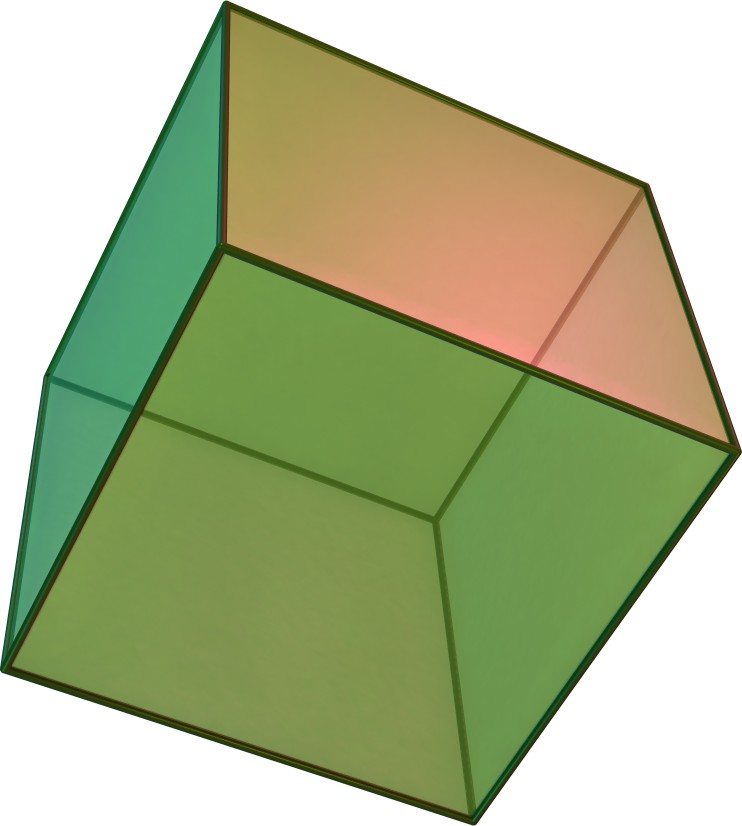
\includegraphics[width=0.5\textwidth]{img/cube.jpg} 
%\captionsetup{justification=centering}
\caption{Cube \cite{FileHexa46online}}
\label{fig:cube}
%license: This file is licensed under the Creative Commons Attribution-Share Alike 3.0 Unported license.
\end{figure}

\cite{hamid2009review} provides a review of various GPU-based sound processing algorithms. Here we will focus solely on those that can be used for spatial audio processes. As Hamid et al. note, digital signal processing (DSP) functions are suitable for GPU-based processing since they are parallelizable, arithmetically intense, have limited data dependency, and make use of multiply-add (MADD) calculations. Whalen \cite{whalen2005audio} explores using pixel shaders\footnote{A pixel shader, also known as a fragment shader, is a program that dictates the color, brightness, contrast, and other characteristics of a single pixel (fragment). A programmer who specializes is writing pixel shader programs is known as a shading artist.} for executing audio algorithms, and compares GPU to CPU performance. The authors of this study implemented some common music systems like filters and delays. Texture access, which has improved since that study, limited the performance of the filters, when compared to CPU benchmarks. 

\cite{trebien2008real} proposed a GPU-based method for real-time sound generation of multi-channel audio. For certain algorithms, the GPU showed speed-ups of up to four orders of magnitude. In other words, the GPU was more than 10,000 times faster than the CPU implementation. \cite{gallo2004efficient} considered variable delay-line and filtering algorithms, both common to spatialization, using GPUs. Delaying the signal was accomplished via texture re-sampling, while filtering was performed using a four-band equalizer. Sound signals were stored as RGBA textures where each component head a band-pass version of the original signal. 

Despite the increase performance, Gallo and Tsingos noted the shortcomings of the GPU-based implementation. Namely, long 1D textures cannot be accessed easily, and IIR filters cannot be implemented efficiently. Also, the GPU only supported 8-bit mixing, which degraded the sound quality. It should be noted that this experiment was conducted in 2004, recent developments in GPU-based spatial audio algorithms have improved performance. Just as recently as 2015, Belloch et al. \cite{belloch2014multi} showed a parallel IIR filter implementation that runs on a GPU, which was used to equalize a WFS system. The implementation ran 1256 simultaneous IIR filters of 256 samples each in real-time with a latency time of 0.72 ms.  

GPUs have also been tested in convolution operation for binaural synthesis by several authors. \cite{cowan2009real} presented a GPU-based convolution method for spatial auditory cue rendering in video games and virtual environments. The comparison showed a processing time of 2-4 ms, depending on graphics card, compared to 4-25 ms on the CPU. A range of signals of lengths spanning from 5,000 to 60,000 explains why the CPU performance varied so much. With a constant running time of 2 ms for convolution the tested video card was shown to be suitable for auralization of FX and music. 

Personalized HRTFs have been shown to improve localization, especially with regard to elevation \cite{kapralos2008virtual}. In \cite{rober2006hrtf}, Röber et al. described an alternative approach to measuring personalized HRTFs in which GPU-based ray-tracing techniques using a 3D mesh model are used to approximate HRTFs. This experiment lacked verification of the method and the diffraction effects of the head were not taken into account. \cite{sung2013individualized} recently conducted a similar experiment in which they improved the ray tracing algorithm to include diffraction at low frequencies and furthermore verified the results using objective measures. Much more recently, in 2020, Guezenoc and Séguier \cite{guezenoc2020hrtf} published a complete survey of HRTF Individualization discussing the most up-to-date work involving both four different types of HRTF individualization methods: 

\begin{enumerate}
    \item \textbf{Acoustic measurement:} acoustic method wherein impulse responses are gathered using in-ear microphones and grids of loudspeakers. 
    \item \textbf{Numerical simulation:} using 3D scans of human subjects. 3D scans can be taken using low-cost consumer grade smartphones \cite{kaneko2016deepearnet}. 
    \item \textbf{Indirect individualization based on anthropometric data:} 
    \begin{enumerate}
        \item \textbf{Adaptation:} using anthropomorphic features of the subject, a generic, or pre-existing HRTF set is modified. 
        \item \textbf{Selection:} using a data set which includes anthropomorphic information, a specific pre-measured HRTF set is selected. 
        \item \textbf{Regression:} the HRTF set is estimated using morphological measurements. A statistical approaches are used to derive the set. Some neural network approaches have been considered.
    \end{enumerate}
    \item \textbf{Indirect individualization based on perceptual feedback:} 
    \begin{enumerate}
        \item \textbf{Selection:} perceptual evaluation task is undertaken by the subject to help select the best HRTF set from the data set.
        \item \textbf{Adaption:} based on responses from subjective evaluation, a HRTF set is adapted using frequency scaling, filter-tuning, or statistical-tuning. \footnote{Refer to \cite{guezenoc2020hrtf} for more details on these three methods.} 
    \end{enumerate}
\end{enumerate}

\todo[inline]{hamidi-2009-gpu-spat-snd-review.pdf Continue 3.1. GPU-Based Acoustical Modeling - Modeling the RIR.}

\todo[inline]{Haven't talked about culling at all yet. see hacihabiboglu-2017-spat-audio-rec-sim-ren.pdf}


\section{Open Tools for Spatial Music} \label{sec:open_tools_spat_mus}
% This section will provide an overview of different existing tools for computer musicians which facilitate the creation of spatial music. We will focus on free and open source tools which work in conjunction with computer music languages such as Pd, SuperCollider, Csound, etc. 

Composers interested in working with computers are well aware of the various different ecosystems existing for the creation of computer-music works. A short list of these systems include: Puredata (Pd), SuperCollider, csound, MAX/MSP, RTcmix, and ChucK. 

In this section we will focus on Pd available tools for creation of spatial works given our familiarity with the system, as well as it's free and open-source nature. Even by focusing only on Pd, there are a slew of available tools that people have developed and published, here we will try to focus on those we find most comprehensive and well supported. 

Our motivation for using FOSS is to democratize access to art-making solutions and consider ways in which we can include as many students as possible into the spatial music-making process. While there are more sophisticated tools out there for making spatial music which one can purchase, we wanted to focus on improvements that can be made to FOSS to bring them up to par with the best commercial systems. 

\subsection{VBAP} 
Vector Based Amplitude Panning (VBAP) is an algorithm written by Ville Pulkki \cite{pulkki1997virtual}. The main drawback of this system is that there is no dedicated binaural rendering system, so it requires a collection of speakers in order to develop the works. One could use a binaural renderer such as \texttt{earplug\~} but there is no obvious way to use a head-tracker, which means the user will need access to a multi-channel sound system. 

The benefit of VBAP is that it is re-configurable to any speaker format, much like ambisonics. The added benefit of ambisonics is that the soundfield can be manipulated using a number of linear transformations which we will discuss later. VBAP is extremely simple to install and operate. 

With Pd installed, the user can simply search for the VBAP externals by typing VBAP under the "Find externals" option in \texttt{Help}. After installing, we recommend shutting down Pd and re-launching it. Make note of where Pd offers to install VBAP. It may suggest installing it inside the Pd app itself. This is a good option because it means one does not need to specify a path to the externals, Pd will automatically know where to find them. The drawback is if one installs a new version of Pd, and deletes the old, you will have to remember to download VBAP again. Alternatively, you can specify a folder of your own choosing and point Pd to it, using the \texttt{Path...} settings under preferences, or by invoking the \textit{[declare]} object in pd.

With VBAP installed now go to \texttt{Help > Browser > vbap} and open up \texttt{vbap-help.pd} to get started. Figure \ref{fig:vbap-5.0} shows an example of using VBAP for a 5.0 set-up\footnote{The example says it is 5.1 but as you can see the sub channel is missing.}. The speaker angles are specified in 2D. The \texttt{vbap} object spits out a list of gain values for each speaker in the order they were specified by the \texttt{define\_loudspeakers} message\footnote{Remember to enable as many speakers as needed under \texttt{Media > Audio Settings} by changing output channels to the desired number.}.

\begin{figure}[ht!]%force figure here, top, strict
\centering
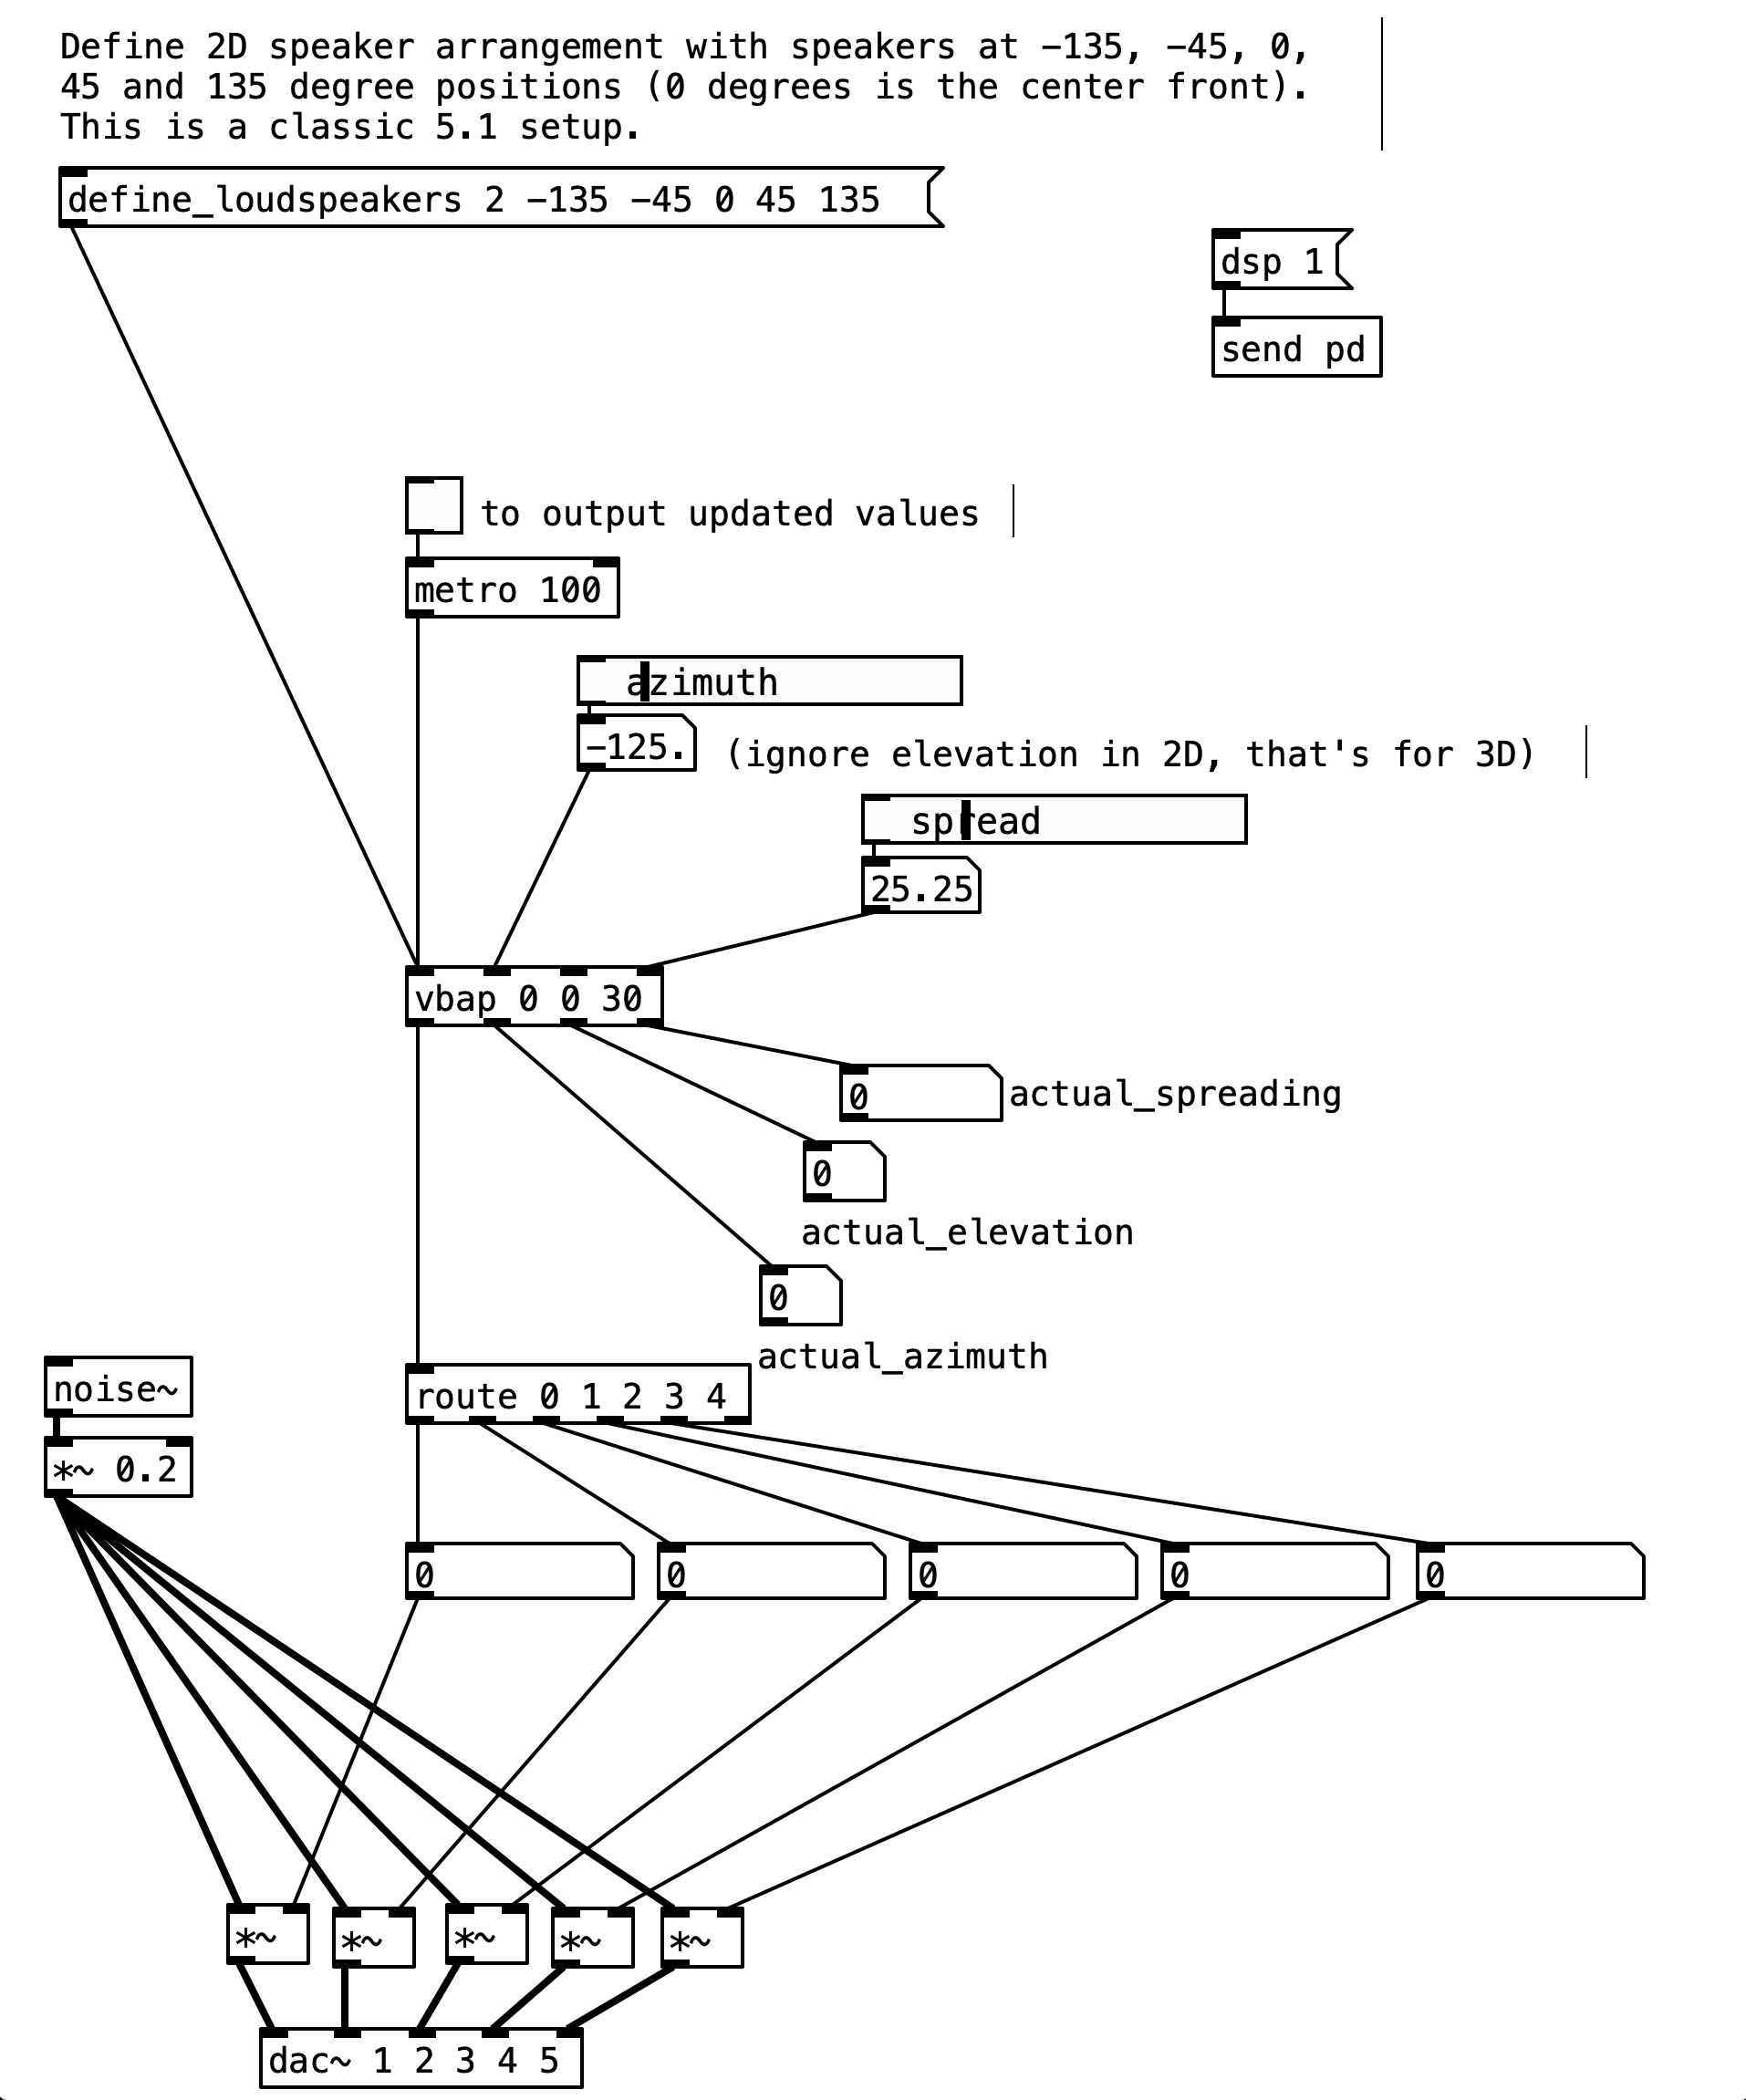
\includegraphics[width=0.7\textwidth]{img/vbap-5.1.png} 
%\captionsetup{justification=centering}
\caption{VBAP 5.0 example}
\label{fig:vbap-5.0}
%license: cc by sa 3.0
\end{figure}

In the example shown the speakers are set up in a quadraphonic arrangement with an extra speaker in the center. It does not follow the International Telecommunications Union (ITU) standard for 5.1 systems \cite{series2010multichannel} for the angles of the speakers. The ordering is also different that the standard. One has to be careful with the routing and ordering of signals, as well as angles, for good multi-channel sound reproduction. It is more common to use the ordering L/C/R/LS/RS\footnote{Left, Center, Right, Left-Surround, Right-Surround} in this format. In the example provided the order is LS/L/C/R/RS instead. 

\begin{figure}[ht!]%force figure here, top, strict
\centering
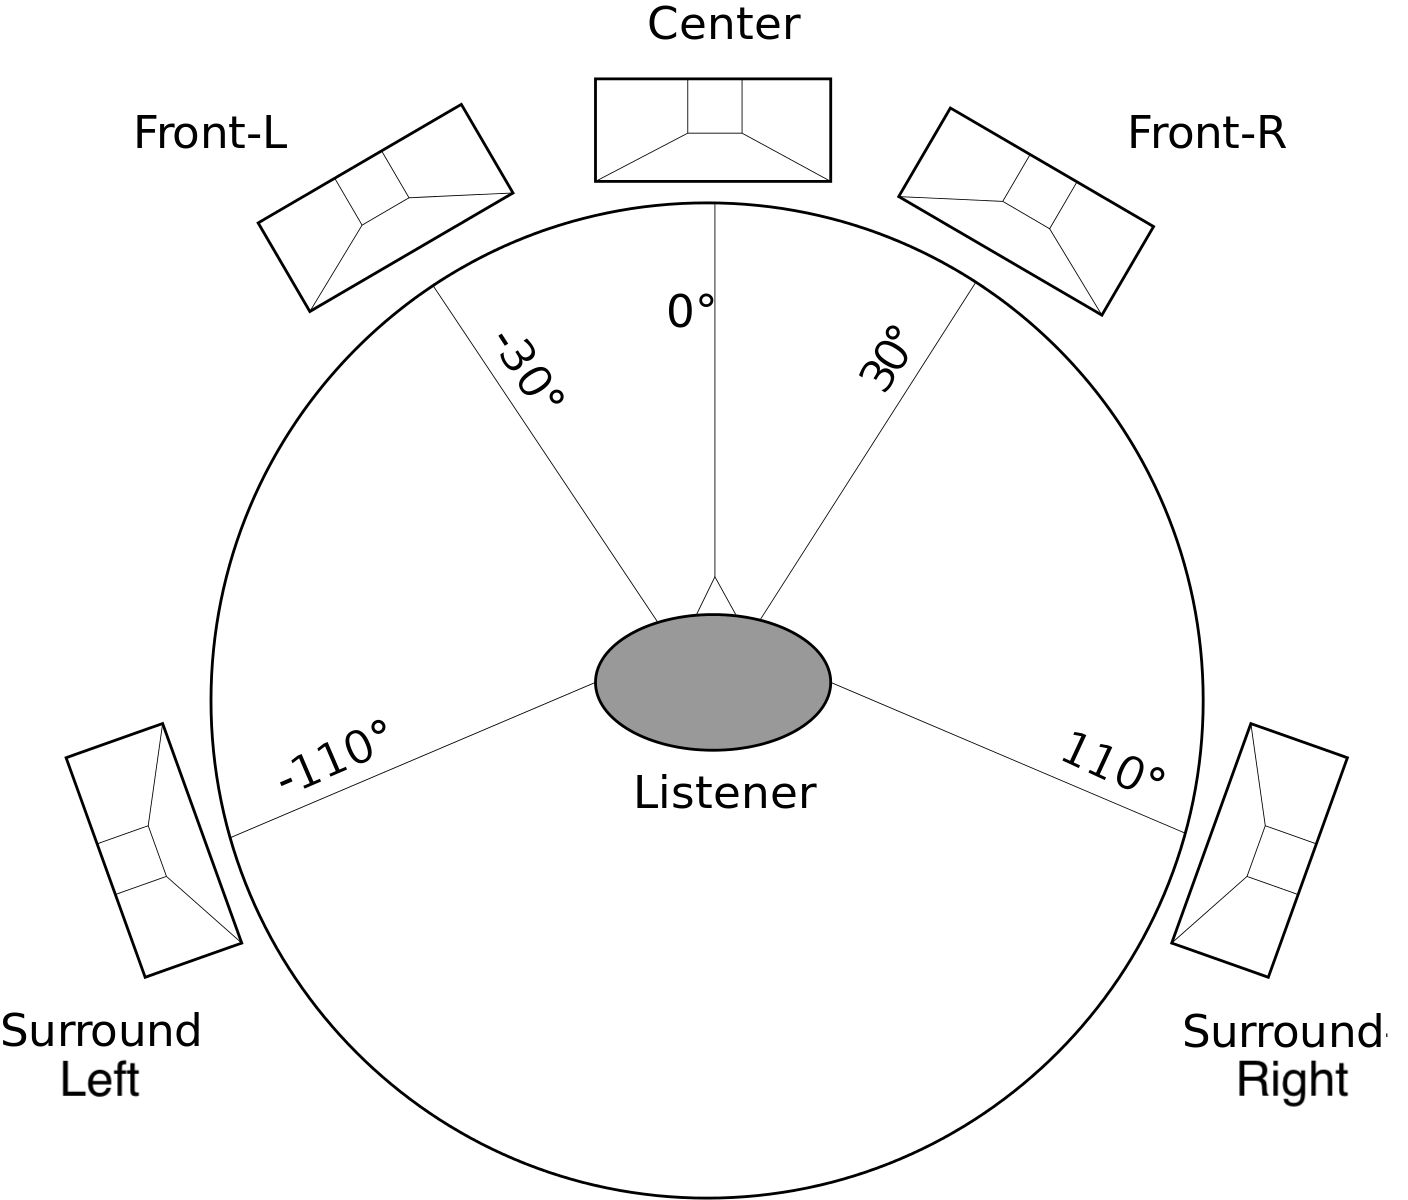
\includegraphics[width=0.5\textwidth]{img/5-1-surr.png} 
%\captionsetup{justification=centering}
\caption{ITU Standard 5.1 surround \cite{File51su81-online}}
\label{fig:5-1-itu}
%license: This file is licensed under the Creative Commons Attribution-Share Alike 3.0 Unported license.
\end{figure}

\todo[inline]{The image is cut off, I have to replace it.}

One of the main drawbacks of this is the fact that if we wanted to change from a 5.0 system to something much larger, like 22.2, we will have to manually route each gain value to its own multiply object. It is possible to use an external library with matrix operations to make things a bit simpler but for most non-experts this will likely prove too complex. Adding height is relatively simple, the message sent to the \texttt{vbap} object has to be sent a modified \texttt{define\_loudspeakers} message where the first argument is 3, which specifies 3D coordinate. The pairs of number following designate the azimuth and elevation of each speaker. 

The vbap folder also has a second abstraction called texttt{[rvbap]} which is meant to add distance effects to the signal. In our trials this external caused Pd to crash, so we recommend sticking with \texttt{[vbap]} instead and adding one's own reverb unit before the panning algorithm. This is far cheaper computationally than applying a reverb to each copy of your signal. Pd vanilla comes with 3 built-in reverb units \texttt{[rev1~]}, \texttt{[rev2~]}, and \texttt{[rev3~]}. Any one of these can be used in conjunction with VBAP to simulate distance. We recommend using a dry/wet control to dictate the simulated distance. 

\subsection{iem\_ambi}

Institute for Electronic Music and Acoustics (IEM) in Graz, Austria, has developed another useful spatialization tool for Pd. Much like VBAP this tool can also be found easily in Pd via the \texttt{Find externals} option in \texttt{Help}. Unlike, VBAP, this ambisonic toolkit is far less intuitive to operate but it does provide some improvements over VBAP. 

Perhaps the most important of these benefits is the fact that ambisonic files can be uploaded and played back over the web in scenarios where asynchronous demonstrations of spatial music are needed. The second benefit, is that a rotation on a soundfield is a linear, non-destructive, transformation which allows us to easily binaurally audition our soundfield without the need for loudspeakers. Finally, there are

\todo[inline]{According to pysiewicz-2016-spat-inst-chapter.pdf the label diffusion is specific to stereophonic sound projection and loudspeaker orchestras. However, in lynch-2017-engulfment.pdf it says "Sound diffusion refers to the practice of localizing and moving sound throughout a space using multiple loudspeakers." }


\section{Spatial Instruments}

This section will discuss the development of \textit{spatial instruments} in the 20th and 21st century. The term \textit{spatial instrument} refers to instruments which allow the user to manipulate spatial elements of sound. Spatial elements might include: direction, reverberance, width, etc. Traditional instruments generally allow the performer control over dynamics, pitch, and sometimes timbre. In contrast, \textit{spatial instrument} give the performer additional control, thus allowing the user to modify the position of sound in space whether that be for multi-channel sound reproduction or binaural synthesis\footnote{Virtual surround sound over headphones.}. 

Many instruments of this nature have been developed over the last few decades due to the popularity of multi-channel reproduction in electro-acoustic music. The development of such instruments goes back to the 1950s, with pioneering works by composers such as Pierre Schaeffer. In contrast to our common definition of instruments, many of the interfaces which will be described in this section do not produce sound at all. In fact, much of the development in Human Computer Interaction (HCI) has focused solely on the manipulation of sounds in space as separate practice from mapping controls to sound synthesis methods.  

\cite{pysiewicz2017instruments} presented a comprehensive ethnomusicological review of \textit{spatial instruments}. In that reference, the authors described a \textit{taxonomy} for the different types of spatial instruments. The five main categories from the 31 different spatialization interfaces found were: 

\begin{enumerate}
    \item \textbf{Instrument-like and augmented controllers:} simulating, inspired, or augmented with traditional/extended techniques. 
    \item \textbf{Touch controllers:} haptic/tactile interfaces.
    \item \textbf{Non-contact, extended range controllers:} free gestures in a limited sense range. 
    \item \textbf{Wearable or immersive controllers:} gloves, suits, camera tracking; performer always in sensing range.
    \item \textbf{Mixed controllers}
\end{enumerate}

Given the comprehensive work undertaken by Pysiewicz et al. we will adopt their taxonomy in our review. In addition, we will seek to integrate some examples that may be missing from the taxonomy based on research published since the aforementioned chapter was published. We strongly recommend Pysiewicz et al.'s chapter for anybody interested in spatial instrument design. In their paper, the authors further sub-divide instruments into three categories based on what spatial parameters they control. Given the ambiguity of these categorizations we have opted not to make such distinctions. One further classification however did seem useful: exclusive spatial control versus hybrid instruments featuring \textit{spatial-synthesis} \footnote{This categorization can be hard to demarcate. In general if one can entirely separate the composition process from the spatialization process, we could argue that the apparatus used for the diffusion of sound does not conform to our spatial-synthesis label.}. We will attempt to highlight spatial-synthesis instruments as we believe these constitute a more interesting family of instruments, rich with creative design possibilities for computer musicians.

\subsection{Instrument-like and Augmented Controllers}

This category refers to instruments which resemble typical musical instruments extended via the use of additional sensors. In this category Pysiewicz et al. only point out two instruments: 

\begin{enumerate}
    \item \textbf{DJ Spat:} by Marentakis et al. (2007) which extends the turntable by using motion-tracking sensors and haptic controls. The angular displacement of the performer's hand is mapped to the sound source position reproduced through a circular loudspeaker array. 
    \item \textbf{Radiodrum:} by Ness et al. (2011), is an instrument used exclusively for spatialization inspired by the radiodrum developed at Bell Laboratories in the 80's. The radiodrum uses capacitive sensing to report the position of two batons in 3D space, as well as velocity when in percussion mode. It is also known as a \textit{radio baton.} Figure \ref{fig:baton} shows Max Matthews, one of the most important figures in computer music, holding a Radio Baton.
\end{enumerate}

\begin{figure}[ht!]%force figure here, top, strict
\centering
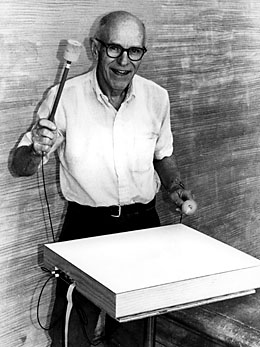
\includegraphics[width=0.5\textwidth]{img/mathews260.jpg} 
%\captionsetup{justification=centering}
\caption{Matthews waving Radio-Baton \cite{FileMath82online}}
\label{fig:baton}
%license: public domain
\end{figure}

Graham \cite{graham2014gesture} presented in 2014 an extended guitar with hexaphonic pick-ups\footnote{A special pick-up for electric guitar with discrete outputs for each string.} which uses a boids algorithm to spatialize sounds. The boids algorithm, developed by CW Reynolds, simulates the motion of flocks of birds. The discrete channels of the guitar output are also analyzed in Pd. Finally, the system includes the use of a Microsoft Xbox Kinect sensor, an infrared depth-sending device, which tracks the guitarists body.

Werner \cite{wernerdevelopment} also published some literature on a similar project entitled GASP or Guitars with Ambisonics Spatial Performance in 2020. This project, from the University of Derby, supervised by Bruce Wiggins, does not use a kinect, but relies only on a MIDI footswitch controller and a hexaphonic pick-up (either the Ubertar hex passive pick-ups\footnote{http://www.ubertar.com/hexaphonic/} or the Cycfi Nu-Series\footnote{https://www.cycfi.com/projects/nu-series/}). One noteworthy element is the creation of a "Guitarpeggiator" which was implemented using gate switching. This allows the guitarist to play arpeggios on the guitar by simply strumming a chord. 

Werner also notes that a cheaper version of this project, not relying on hexaphonic pickups, could be achieved using some frequency splitting\footnote{This might work in harmonic sections, but is unlikely to work in melodic phrasing. This is because the frequency range of individual each string might not cover the entire audible spectrum.}. The author's future work includes integrating the entire system into a single application. Currently it relies on mostly FOSS, with the except of the DAWs for ambisonic processing and MIDI event triggering (for the arpeggiation). 

\subsection{Touch Controllers} %haptic/tactile

This category refers to instruments which need to be physically interacted with, in a tactile fashion, for operation. This can include touch screen like those found in tablets or something simpler like a potentiometer or button. Same of the earliest examples of spatial instruments made use of tactile interfaces, thus, a number of historical examples will be present in this section. Below we provide a list of some of the most noteworthy examples from \cite{pysiewicz2017instruments}.

\begin{enumerate}
    \item \textbf{Sal Mar Construction:} designed in the early 1970s by composer Salvatore Martirano (USA), the instrument is a analog/digital composition machine which featured 24 spatialized audio channels. Figure \ref{fig:sal-mar} depicts the instrument (photo courtesy of the University of Illinois).
    
    \item \textbf{Hybrid IV:} developed by Edward Kobrin\footnote{Very little information could be found online about Kobrin. \cite{kobrin1968solution} suggests he was American, since this work was conducted at Northwestern University, Evanston, Illinois.} in 1975, the systems sound-making components are analog but the score is composed using digital means. The multi-channel matrix provides 16 outputs. 
    
    \item \textbf{SSSP Sound Distribution System:} developed by Guy Fedorkow et al. in the late 70s at the University of Toronto, Ontario, Canada. In contrast to the two previous examples the system was modular in nature: the polyphonic sounds are synthesized by one module and controlled spatially by another. It also featured a keyboard, tablet, and 16 outputs. 
\end{enumerate}

\begin{figure}[ht!]%force figure here, top, strict
\centering
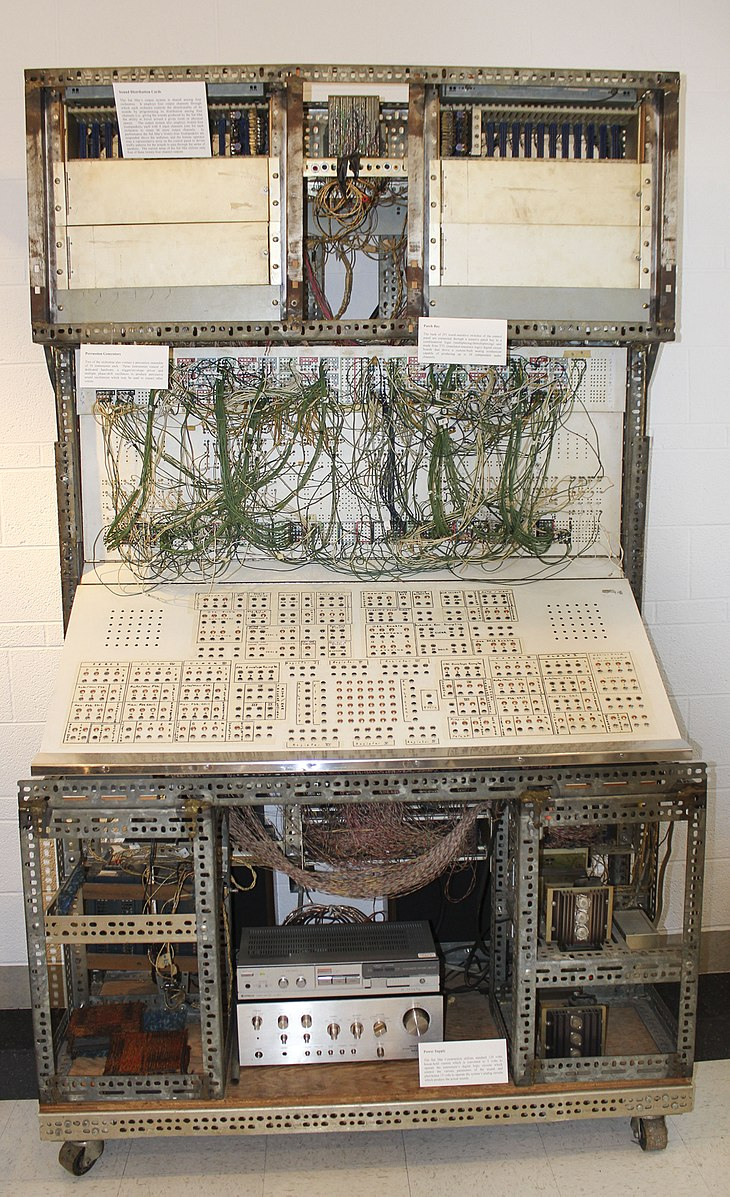
\includegraphics[width=0.5\textwidth]{img/sal-mar.jpg} 
%\captionsetup{justification=centering}
\caption{Sal Mar Construction \cite{FileTheS26online}}
\label{fig:sal-mar}
%license: This file is licensed under the Creative Commons Attribution 2.0 Generic license.	
\end{figure}

All three of these examples fall under the spatial-synthesis category, wherein synthesis and spatial control are integrated into a single instrument. The following examples are of instruments used exclusively for the spatial control of sound.

% \todo[inline]{Don't exclude anything, but you don't need details on all the systems.}

\begin{enumerate}

    \item \textbf{HaLaPhon:} invented in the late 1960s by Hans-Peter Haller and Peter Laszlo, the instrument counted with switches and automation for the control of sound diffusion in circular arrangements by employing amplitude panning. The device evolved from analog to digital versions, all maintaining the overall concept.
    
    \item \textbf{Loudspeaker Orchestras:} there are multiple Loudspeaker Orchestras such as the Gmebaphone (1973) (also known as the Cybernephone), the Acousmonium (1974), and the BEAST System (1986). These all share portability as a key feature and an associated fader board system for spatialization. These instruments were developed at Bourges\footnote{France.}, Paris, and Birmingham respectively. The speaker arrangements are very specific, in contrast to other systems.
    
    \todo[inline]{Detail missing here. Composers. Pieces. Loudspeaker Orchestras is huge topic. There is a bit of overlap w/ Ch2 section on electro-acoustic music, try to not repeat yourself, cross-reference instead.}
    
    %% Don't exclude anything, but you don't need details on all the systems. I will make a small list of the things I leave out intentionally.
    
    % \item \textbf{TRAILS:} the Tempo Reale Audio Interactive Location System was created by Bernardini in 1989. It does not define specific speaker layouts.
    
    \item \textbf{Rotation Mill (Tonmühle:} was conceptualized in the 60's at the Technical University of Berlin and later used by Karlheinz Stockhausen for use at the Osaka World Expo in 1970. At the expo the rotational resistance device was patched to 50 loudspeakers surrounding the audience.
    
    %\item \textbf{Circular Relay Switch:} Leitner in 1971 %is this same as bernard leitner from installation works?
    
    \item \textbf{Spherical Sound Controller:} was also designed for the 1970 World Expo, this time for use in the West German pavilion. It was also created by the Electronic Music Studio at the Technically University of Berlin and "consisted of 50 sensor buttons, each representing a loudspeaker group in the spherical concert hall" \cite{pysiewicz2017instruments}. The instrument allowed sources to be projected and moved in space.
    
    %\item \textbf{MusicSpace}
    
    \item \textbf{Expanded Instrument System:} or EIS, for short, was developed by Pauline Oliveiros starting in 1963. It constitutes a performance environment that "intends to give performer control over the acoustic space" \cite{pysiewicz2017instruments}. EIS features: amplitude panning, delays, and a reverb unit, connected to an interface consisting of several footswitches.
    
\end{enumerate}

The above list constitutes some historical examples of tactile interfaces for sound spatialization. Below we will continue with the category focusing on technologies developed in the 21st century\footnote{For sake brevity a few instruments have been left out of our list such as the: \textbf{TRAILS} (Bernardini 1989), \textbf{Circular Relay Switch} (Leitner 1971), and \textbf{MusicSpace} (Pachet and Delerue in 1999).}.

\begin{enumerate}

    \item \textbf{M2:} was created by Mooney in 2004 and presented as a modular diffusion system featuring digital rendering engine and a specifically designed fader board. The system allows for grouping of sound sources which could be a useful feature in these systems. For example one might group all percussive elements together and use a single fader to control their volume.
    
    \item \textbf{Multi-Touch Soundscape Renderer:} \cite{bredies2008multi} was created by Bredies et al. in 2008 and comprises of a multi-touch tabletop used for manipulation of sound objects rendered using WFS via a circular array of speakers. One of the noteworthy elements of this project is the ability for multiple people to interact with the tabletop at once. This particular tabletop was based on the Frustrated Total Internal Reflection (FTIR) technique \cite{han2005low}. The tabletop was built as a testing environment for the Soundscape Renderer\footnote{http://spatialaudio.net/ssr/} (SSR).
    
    \todo[inline]{reactable, audiopad, LEMUR, ISS Cube, Audiocube, IOSONO all in bredies2008multi (bibtex) } 
    
    \todo[inline]{johnson-2014-diffusing-diffusion.pdf}
    
    \item \textbf{Tactile.space:} is another similar project by Johnson and Kapur (2013) which was later expanded into a tablet-based system making it more portable and personalized. The \textbf{tactile.motion} tablet application uses amplitude panning sent via OSC to a main computer for sound spatialization. 
    
    \item \textbf{Sound Surfing Network:} is another mobile spatialization application this time presented by Park et al. (2013). The system is comprised of two cell-phone apps, one for the performer and one for the audience. The audience app "turns each smartphone into an element of the loudspeaker array" \cite{pysiewicz2017instruments}. Unfortunately, cell-phone speakers do not have particularly good frequency response. However, if these small cell-phone speakers were supplemented with an additional pair of bigger speakers, capable of reproducing some of the missing "low-end", this might be a noteworthy experience.
    
    \item \textbf{Sound Flinger:} is a haptic controller for spatial-synthesis control of sound. It was created in 2011 by Carlson et al. This simple design uses just two buttons and four faders to control a physical model in a quadraphonic system. The physical models are accomplished via Edgar Berdahl’s haptic object library \cite{berdahl2010hsp} and runs on a Beagleboard\footnote{https://beagleboard.org/} using a PlanetCCRMA distro\cite{lopez2005surviving}. From an informal survey, users reported the need for the instrument to have a visual representation of sound sources, in order to facilitate playing sounds in space.
    
\end{enumerate}

\subsection{Non-contact, Extended Range Controllers} %free gestures

This section corresponds to instruments which require to physical touch for their operation. This includes systems using either light sensitive receivers or electromagnetic sensors (aka. inductive capacitance). 

\begin{enumerate}
    \item \textbf{Photocell Mixer:} was developed in the 1960s by Frederic Rzewski (1968) and David Behrman (1967). Each composer developed their photocell mixer independently but they both shared the same principles. Panels with photocells are integrated into the signal circuit. Using a penlight, the user can assign signals to loudspeakers by reducing the resistance between components separated by the photoresistors\footnote{A photoresistor is a passive component that decreases resistance with respect to receiving luminosity on the component's sensitive surface.}. 
    
    \item \textbf{Light-Emitting Pen Controller:} was developed by Brown et al. in 2005. In their approach light-emitting pens are captured and tracked in space using computer vision algorithms. Their particular implementation made use of the Jitter visual programming environment included with Cycling 74's MAX/MSP\footnote{https://cycling74.com/products/max/}. 
    
    \item \textbf{Grainstick:} was created by Leslie et al. at IRCAM in 2010 and shows a multi-modal approach to controller systems which employs both infrared motion tracking and accelerometer data. Each grainstick has a number of reflective balls which can be tracked by the infrared sensors in space. The data from both the infrared capture and the accelerometer (from the Wiimote) is used to drive a granular synthesis system using WFS. The synthesis is accomplished using the CataRT Library for MAX/MSP \footnote{http://ismm.ircam.fr/catart/}. There is also some gesture analysis applied to the accelerometer data via the Jamoma\footnote{http://www.jamoma.org/} framework. This instrument also fits within our spatial-synthesis category since each grainstick controls both spatialization and synthesis parameters.
    
    \item \textbf{Pupitre d'Espace:} is perhaps the oldest of all the instruments in our list. It was developed by Pierre Schaeffer in 1952 and operated on the basis of electromagnetic inductance. Four induction coils are mounted around the performer as receiver rings. One additional coil is held in the hand of the performer. The distance between the receiver rings and the moving coil in the performer's hand induces four currents which are used to control the amplitude of four speakers. 
    
    \item \textbf{NAISA:}
    \item \textbf{Gesture Controller for a WFS System}:
    
    \item \textbf{Holistic Spatialisation System for Multiple Sound Sources:} (HSSMSS) is a controller presented by Diatkine et al. in 2015, which makes use of a "short-range infrared sensor" capable of tracking hand gestures and mapping these to musical parameters. The system relies on HOA for the spatialization of sound sources, a LeapMotion\footnote{https://developer.leapmotion.com/} controller, and MAX/MSP as the main environment. It also supports binaural synthesis with head-tracking for auditioning of sound-fields via the \texttt{Sarcoder\~} MAX/MSP external.
\end{enumerate}

\subsection{Wearables or Immersive Controllers} %always in sensing range


\subsection{Mixed Controllers} %no definition


\subsection{VRMIs}
\todo[inline]{For now I am using a separate category. I have to go back and integrate.}

Virtual Reality Musical Instruments (VRMI) (serafin-2016-vr-inst.pdf) constitute a new type of musical instrument that include simulated visual data shown using a HMD or CAVE system. Serafin et al. hypothesize two reasons why perhaps these instruments have been paid less attention:

\begin{enumerate}
    \item Musicians generally rely on sound and touch for performing on their instruments.
    \item Devices providing visual feedback that are both low-cost and portable have only recently become available (ie. Oculus HMDs). 
\end{enumerate}

VRMIs, according to the authors, is limited to visual feedback via an immersive system. In other words, 2D projection of 3D environments is not considered sufficient for an instrument to be considered a VRMI. These multi-modal virtual musical instruments (VMI) are also interesting and often spatial, but not part of a true VR system.

One of the challenging aspects of these instruments is that it is hard for the audience to witness the performance, since the musician is donning a HMD offering a personalized experience. It is possible to project a \textit{monoscopic} view of the performers action, however, the discourse between musician and audience will be lost, to some extent, as the performer will have no sense of his or her surroundings. 

\begin{enumerate}
    \item \textbf{CORDIS-ANIMA:} (Cadoz et al. 1993) this system has never been strictly used as a VRMI but it has all the elements necessary to create a sophisticated VRMI. Namely, it features physical models for both auditory and visual phenomena. 
    
    \item \textbf{}
    
\end{enumerate}

In addition to providing a survey of some VRMIs, Serafin et al. (serafin-2016-vr-inst.pdf) also provide some guiding principles for VRMI design. 

%%%%%%%%%%%%%%%%%%%%%%%%%%%%%%%%%%%%%%%%%%%%%
\section{Open Tools for Spatial Instruments}

\section{The Future of Spatial Music \& Instruments}

\section{Conclusion}



 
%spatial audio (fixed-media) [REC/REPRODUCTION]
\chapter{Spatial Audio: Capture \& Reproduction} \label{ch:spat-aud}

\todo[inline]{I am not sure but I think this chapter is too long. I might need to split it into capture for one chapter and reproduction for another chapter. I can also just put reproduction into chapter 2. It might be ok.}

\section{Introduction}
%This chapter will be developed with Tamara Smyth.

In this chapter, we will shift the focus from spatial music to spatial audio. We will begin by drawing a line from the inception of recorded sound to the latest developments in 3D audio, including advancements in cross-talk cancellation (XTC), WFS, and ambisonics. In this chapter, we are concerned with the variety of ways that sound engineers can use spatial audio technologies to record and reproduce spatial music: whether that be in real-time or asynchronously. We will also touch upon some of the technical complications of this work that might prove problematic for engineers (ie. insufficient memory, speaker count, hardware requirements, etc.).

In particular, this chapter will focus on the main technology this author is concerned with: ambisonics. One of the major benefits of ambisonics is the \textit{isotropic}\footnote{Identical in all directions; invariant concerning direction. In an ambisonic context, this means the sound field can be reproduced in whatever sound system is available.} nature of the design, which makes it more flexible than surround sound standards such as 5.1. Ambisonics has a long-established tradition in the spatial audio community and as such, a myriad of open source tools have already been developed for its usage. These tools make it more accessible in many ways that \textit{object-based audio} (OBA) ecosystems. With the proliferation of systems for binaural rendering, ambisonics has resurfaced as a reliable method for spatial audio reproduction.

In addition to listing and demystifying the different spatial audio technologies available today for playback, we will suggest engineering approaches for the capture of spatial sound both for real-time transmission and for asynchronous dissemination using open-source technologies. We will focus on spatial audio recording techniques and describe systems based on freely available software for mixing and mastering spatial audio which can later be used in immersive environments such as the ones described in Chapter \ref{ch:xr-mus}. In contrast to Chapter \ref{ch:spat-mus}, which outlines technologies which are better suited for real-time performances with musicians, in this chapter we will focus more on tools for creating \textit{fixed-media} works.

\section{History of Spatial Audio Capture and Reproduction}

In the previous section of this paper we presented a number of composers who made space an integral part of their practice as well as \textit{spatial instruments} used for the development of such works. This next section will describe the development of modern spatial audio systems from an historical and engineering perspective. 

% Many engineers must be thanked for giving composers the ability to \textit{diffuse} sound in space towards musical ends. In this section we will discuss some of the most influential engineers that have contributed to the development modern \textit{spatial audio} systems. 

% The chapter will be divided into four sections: 

% \begin{enumerate}
%     \item Spatial audio developments before the 21st century
%     \item Contemporary spatial audio developments in sound recording
%     \item Contemporary spatial audio developments in sound reproduction
%     \item Overview of open tools for recording and playback of spatial sound
% \end{enumerate} 

\subsection{Audio Pioneers} \label{subsec:audio_pioneers}

The invention of the telephone, in 1876, by  Alexander Graham Bell \cite{grosvenor2016alexander}) can be considered the genesis of all \textit{spatial audio} technologies. The transmission principles it used where what later inspired the development of the phonograph, one of the first known recording devices, invented by Thomas Edison in 1877 \cite{gitelman1999scripts}, and, subsequently, galvanized a whole new generation of engineers who developed more sophisticated methods for sound capture and reproduction. 

\begin{figure}[ht]%force figure here, top, 
\centering
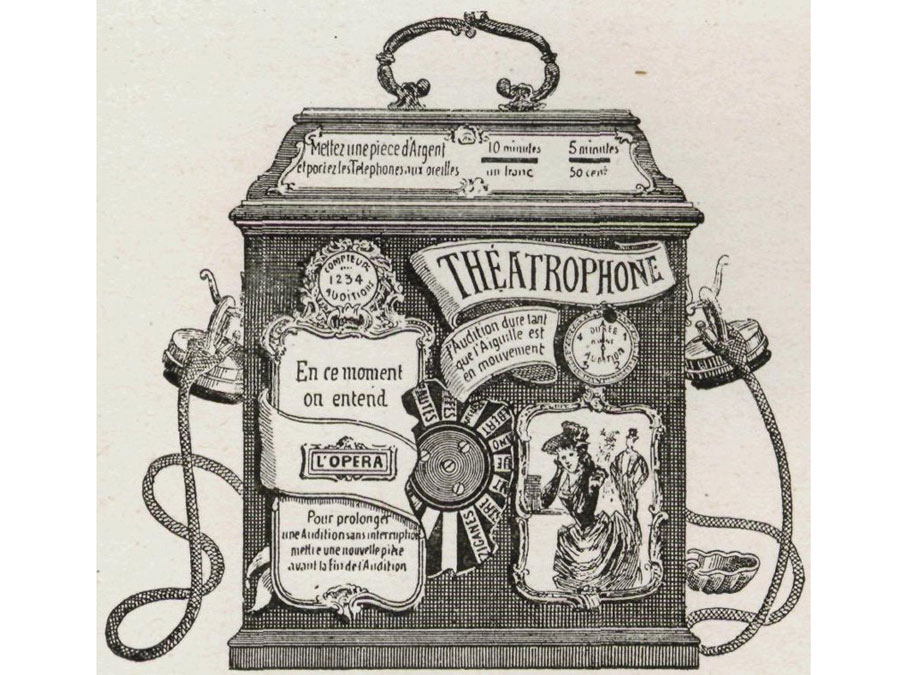
\includegraphics[width=0.7\textwidth]{img/theatrophone.jpeg} 
%\captionsetup{justification=centering}
\label{fig:theatrophone}
\caption{Théâtrophone \cite{theatrophone_pic}}
\end{figure}

A few years after the invention of recorded sound, Clement Ader, best known for his work in  aviation, would present the \textit{théâtrophone}, a "system of telephonic transmission where listeners received a separate channel for each ear, enabling stereophonic perception of actors on a set" during opera performances. Just a year before, Ader had presented his prototype at the Paris Exhibition for Electricity in 1881 \cite{malham19953}. Figure  \ref{fig:theatrophone} shows a picture of the device. We can see the two receivers which would be placed at the listeners ears for \textit{stereophonic} audition. The writing on the image also shows the cost for the audience member, which was 10 minutes for one franc, or 5 minutes, for 50 cents. This device should not be confused with the additive synthesizer entitled \textit{Telharmonium} by Cahill, described in Chapter \ref{ch:spat-mus}. 

Decades would pass before any new major developments in the field would occur, but eventually, in the 1920's, Harvey Fletcher, from Bell Telephone Laboratories\footnote{Bell labs has an important place in computer music history. It is where Max Mathews wrote the first computer music language, MUSIC-N.}, developed one of the first binaural recording systems. This system used the anatomy of the head to naturally embed spatial attributes of sound to recordings \cite{harvey1927binaural}. It would not be, however, until 1933, at the Chicago Century of Progress Exhibition, that binaural recordings would first be introduced to the public. 

Fletcher is believed to also be responsible for the first public demonstration of stereophonic sound, which took place in 1934 in New York City. Bell Telephone Laboratories, along with Fletcher, is also accredited for, in the 20's, being the first American institutions to research what is known today as wave-field synthesis (WFS): a system which captures a "wall of sound", using an array of microphones, and then consequently plays it back, using an array of speakers. In other words, engineers would mount a curtain of microphones and then reproduce the recorded signals using a curtain of speakers of similar proportions\cite{fletcher1942hearing}\footnote{While Fletcher would be one of the first to describe the idea of WFS in 1942, it would not be until 1988 that Berkhout would propose the mathematics involved in WFS to transform a single sound source into a wall of sound.}.

Later, in 1933, Fletcher also demonstrated the possibilities of long-distance multi-channel sound transmission. In a collaboration with English conductor Leopold Stokowski, considered one of the first stereo control-board operators\cite{mcginn1983stokowski}, Harvey and other Bell Lab engineers put together a system which transmitted the sound of an orchestra in Philadelphia via three microphones placed on stage to three corresponding loudspeakers in Washington DC's Constitution Hall. Bell Labs and Stokowski would go on to collaborate on numerous events in the 40's. Around the same time Alan Blumlein, an American engineer, was working on a much simpler yet powerful spatial audio technique: high-fidelity stereophony. 

Blumlein's most important contribution to the field of spatial audio is perhaps his mid-side (MS) encoding technique, patented in 1931 \cite{billingsley1987simulated}. This technique allowed audio engineers to mix stereo and mono information,  towards spread control, by summing and subtracting signals with equal and inverted phase. The technique was later expanded by Gerzon to develop a First Order Ambisonic\footnote{Also known as tetrahedral microphone} microphone. The idea consisted of taking the output of a \textit{figure-8} microphone and summing it with an \textit{omni-directional} microphone. A second copy of the figure-8 microphone would be phase inverted. The result were two cardioid like patterns with the same orientation as the stereo-speaker arrangement. Figure \ref{fig:ms_stereo} shows the general set-up for the MS stereo recording technique, note the panning on the two copies of the figure-8 microphone. 

\begin{figure}[h!]%force figure here, top, strict
\centering
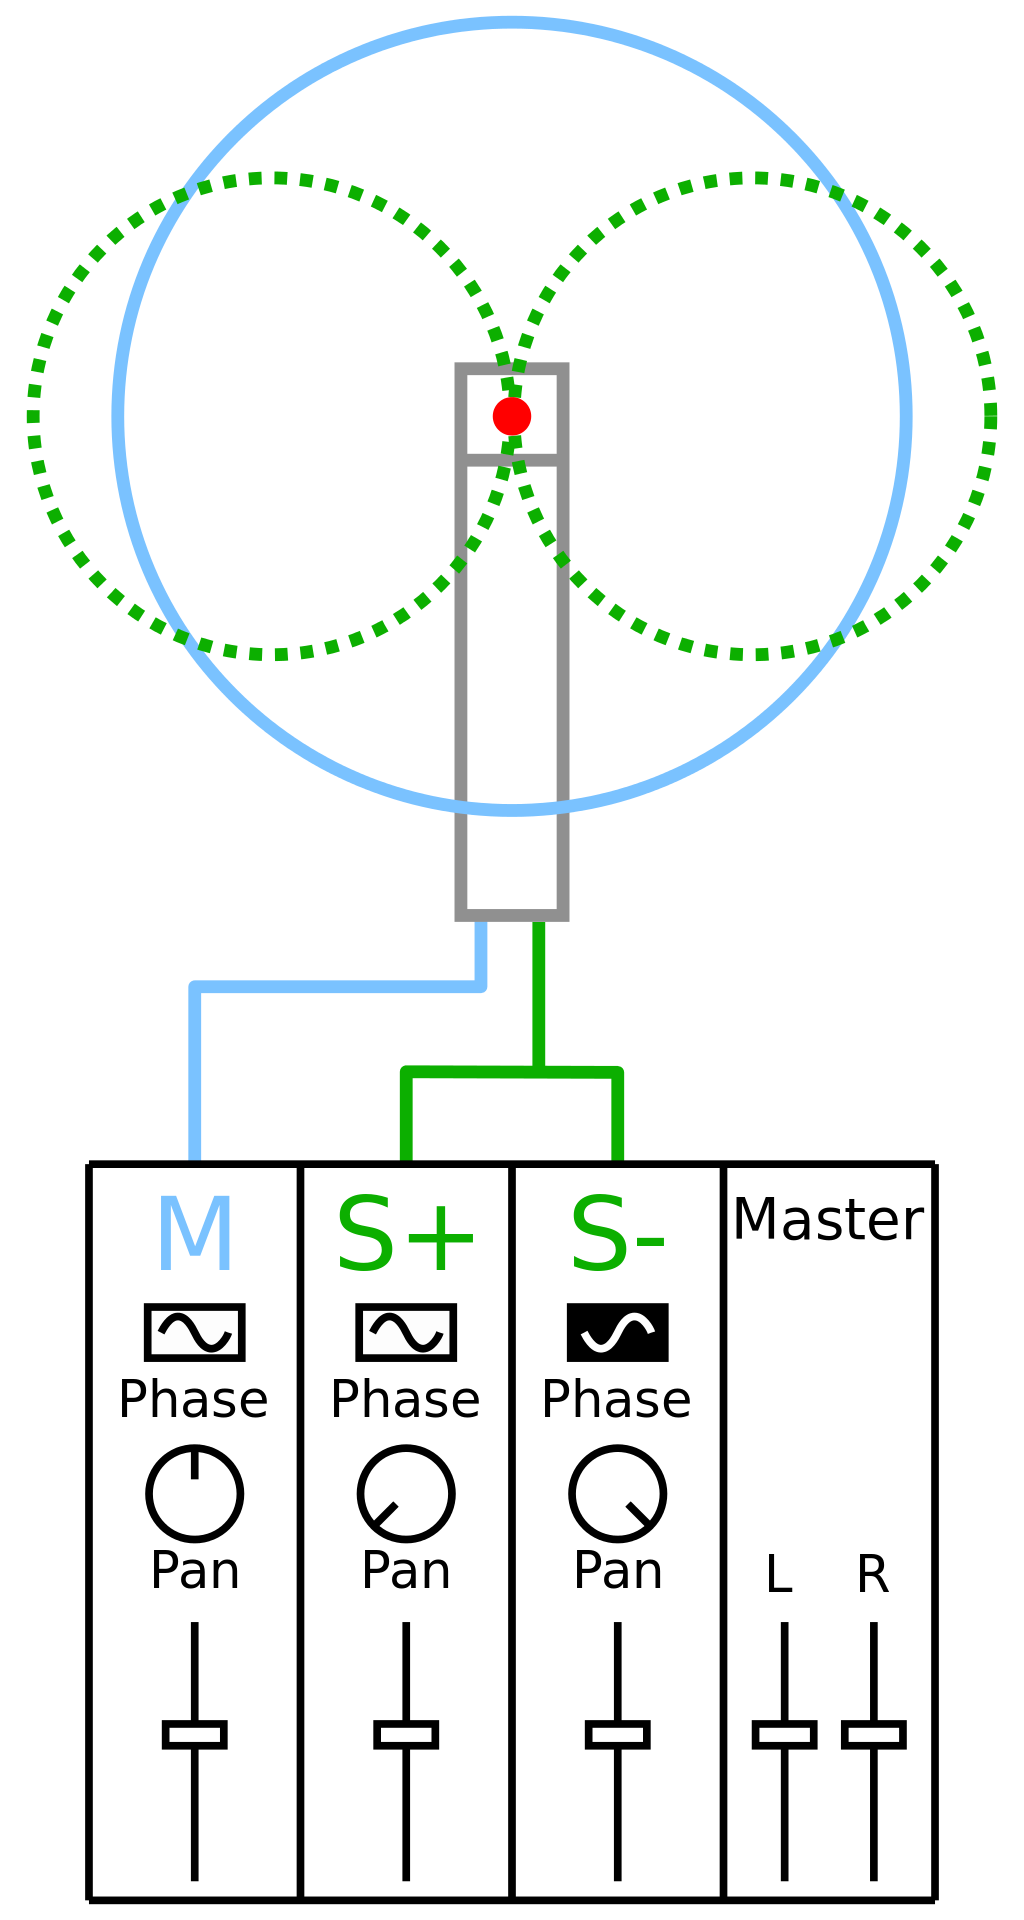
\includegraphics[width=0.35\textwidth]{img/ms_stereo.svg.png} 
%\captionsetup{justification=centering}
\label{fig:ms_stereo}
\caption{Mid-Side Stereo \cite{ms_stereo_pic}}
\end{figure}

One of the biggest moments for spatial audio occurred at the very end of the decade. In 1940, Leopold Stokowski, RCA, and Disney would release the film \textit{Fantasia} which featured a system called \textit{Fantasound}. The control system they designed allowed audio tracks to be panned to any of 10 loudspeakers \cite{klapholz1991fantasia}. This lead to an era of development in professional theatre systems with much to be desired on the consumer end. Moderate improvements to sound quality and storage capacity were achieved from 1940 to 1970.

In the 1970's, a new and significantly more obscure technology began being developed: \textit{quadraphonic sound}. Quadraphonic research is believed to have begun at the Acoustic Research Corporation by Robert Berkovitz \cite{davis2003history}. The idea was to use two rear channels commercially to produce the ambience of the recording and two front channels for direct sound. Unfortunately, due to a number of financial, engineering, and marketing issues, the system never gained much popularity. Fortunately, the system did inspire other developments. 

The development of encoding and decoding schemes for quadraphonic sound would eventually peak the interest of British mathematician Michael Gerzon. Michael would, in 1969, present to the public a new audio capture method inspired by Alan Blumlein and the rise of interest in quadraphonics. Gerzon proposed, provocatively, the use of a tetrahedral array for audio capture in which the four signals could be encoded into three coincident\footnote{Coincident here meaning placed close together.} figure-8 microphones. This system, Gerzon believed, could optimize the use of the four speakers by providing listeners with not only horizontal information, but also vertical sound. Unfortunately, the system suffered from a considerably small ideal listening area\footnote{Also called \textit{sweet spot}. Higher Order Ambisonics (HOA) has been shown to increase the size of the sweet spot.}, a fact which detracted sound system engineers who were primarily concerned with audio for film, as it had become, and possibly remains, the focus of spatial audio research. 

Around the same time, in 1970, Tom Horall of what today is known as Acentech\footnote{https://www.acentech.com/} decided to attempt to recreate the acoustics of the famous Boston Symphony Hall using a acoustic model approximation. The system used tape delay techniques to achieve believable spatial sound. Using a dozen loudspeakers Horall was able to convince the listeners that they were actually being transported to the iconic hall. The system would later be commercialized in 1988 and become known as the Pioneer DSP-3000 \cite{davis2003history}. 

Many other developments followed suit from the 80's to today. Perhaps the most popular of these is 5.1 surround sound, a popular audio system which has had decent success commercially. Today, there is an ongoing battle regarding the future of spatial audio. Companies are consistently looking for scalable and reliable solutions to improve sound quality for patrons. Unfortunately, many of these systems have suffered from their distinctly complicated set-up process or high costs. The quest for: simple, high-fidelity, three-dimensional sound; is one that will, likely, not end soon. 

%\subsection{Stereo Techniques}
\subsection{Binaural Microphones}

\textit{Binaural audio} and \textit{multi-channel stereophony} are the two most common spatial audio technologies. \textit{Binaural audio} has become increasingly popular for \textit{virtual reality} (VR) while \textit{multi-channel stereophony} can be found in home entertainment systems as well as automotive sound systems. Stereo, however, is still the prevailing reproduction format, which is why binaural microphones have gotten some interest as a means of "static" spatial audio reproduction. Others have written about \textit{transaural} sound systems, which reproduce \textit{binaural audio} over stereo systems. \textit{Transaural} reproduction is a niche system that has been gaining more interest in the community. The underlying technology, however, seems to remain limited to audiophiles and a number of select engineers working on it.

In contrast to other spatial audio recording methods which rely on large arrays of microphones binaural recordings only use two microphones to encode spatial information into a stereo recording. Binaural recordings are either captured using a \textit{dummy-head}, a mannequin head with microphones inside its ears, or with \textit{in-ear} microphones placed inside a person's ear canals, to capture what they would normally listen to. By playing back these binaural recordings using headphones, ear-buds, or with stereo speakers using \textit{cross-talk cancellation} (XTC) filters\footnote{XTC is also referred to as \textit{transaural reproduction} in the literature.}, a person can sense a sonic space around them as it originally occurred. 

Unfortunately, some issues arise from this method. Firstly, people's heads and ears differ in size and shape, a fact which distorts the recordings ever so slightly breaking the illusion that one has been transported from their current location to the new auditory scene. Secondly, when the listener hears back the recording, they will be striped of rotational control. In other words, when they turn their heads, the sound will remain fixed in the same perspective as the original recording, and the illusion of immersion will be lost. This lack of \textit{auditory parallax} creates localization errors and \textit{internalization} of sound sources. Figure \ref{fig:dummy-head} shows a "dummy head" - a binaural microphone with two capsules placed inside the modeled pinnae, mimicking the behavior of the human cochlea\footnote{The biological structure in our inner ear where frequency analysis is performed.}. The \textit{pinnae} in these systems tends to be manufactured using a soft plastic such as silicone to mimic the absorption of human cartilage on sound.

\begin{figure}[ht!]%force figure here, top, strict
\centering
\includegraphics[width=0.7\textwidth]{img/dummy-head.jpg} 
%\captionsetup{justification=centering}
\label{fig:dummy-head}
\caption{Dummy Head - wikimedia commons}
\end{figure}

\textit{Binaural recordings} are not a particularly good representation of the desired sound-field resulting from a \textit{spatial music} work, however, they are crucial for the development of binaural synthesis systems, which ultimately can convey a proper representation of the musical work. Often, it becomes impractical to use a real human for HRTF sampling since the process can take quite a long time and human movements during acoustic sampling can lead to errors in the dataset. In this context, an anthropomorphic average of a human is better suited for the sampling task. Alternatively, the binaural impulse responses can be synthesized using acoustic models. \cite{algazi2002use}, for example, describes a head-and-torse model, or "snowman" model, to efficiently implement HRTF approximations towards real-time spatialization. 

\begin{equation} \label{eq:conv-hrir}
\begin{array}{l}
x_{L}(n)=\sum_{p=1}^{P} x_{p}(n) * h_{L, \theta_{p}, \phi_{p}}(n) \\
x_{R}(n)=\sum_{p=1}^{P} x_{p}(n) * h_{R, \theta_{p}, \phi_{p}}(n)
\end{array}
\end{equation}

\cite{hacihabiboglu2017perceptual} provides a simple equation for the \textit{auralization} of a virtual signal via convolution with two HRIRs. This is equivalent to the process of filtering the source $x_p$ with a filter whose frequency response would be identical to the Fast Fourier Transform (FFT) of $h_{R, \theta_{p}, \phi_{p}}$ and $h_{L, \theta_{p}, \phi_{p}}$ respectively. The topic of \textit{binaural synthesis} will be further discussed in later sections, as it is a primary topic of this work, which warrants extensive discussion.

\subsection{Sound-field microphones}

History of sound-field microphones.

% \subsection{Surround Sound}
% ITU standards, THX, MPEG-H, etc.

\section{Contemporary Spatial Audio Capture Techniques} \label{sec:contemp_audio_capture}

While the popularity of spatial music has become evident in the electro-acoustic domain, little effort seems to have been devoted by composers for the accurate representation of their music in a recorded format. Often, composers opt to use stereo recordings of their work, due to the complexity of spatial audio recording technologies or their lack of availability. While in previous sections of this work we have focused on technologies which allow the creation of spatial music, in this section we will focus on hardware and software which allows one to document their works, with differing degrees spatial quality retained, for public dissemination outside of the concert hall. 

\subsection{Multi-channel Spaced Microphone Arrays}
%https://www.dpamicrophones.com/mic-university/immersive-sound-object-based-audio-and-microphones

Before we can begin to understand contemporary 3D audio capture techniques we should discuss some fundamental microphone principles. All spaced microphone arrays rely on systems which turn air pressure changes into electrical currents and subsequently binary information, which represent these pressure changes as sampled in time. Most well-known \textit{monophonic} microphone types fall within the family of cardioids. The general equation for the family of cardioids is:

\begin{equation}
    \rho(\theta) = \alpha + (1-\alpha)cos(\theta)
\end{equation}

This equation, from \cite{ortolani2015introduction}, provides a way for us to construct the most common types of \textit{polar patterns} found in commercial microphones today. \textit{Polar patterns} depict the sensitivity of a microphone to sound pressure as a function of the direction-of-arrival (DOA) and are frequency dependent. The most important patterns for our purposes are: \textit{omni-directional} where $\alpha=1$ \textit{cardioid} where $\alpha = 0.5$, and \textit{figure-of-eight} where $\alpha=0$. Figures \ref{fig:card}, \ref{fig:omni}, and \ref{fig:fig-8} show the polar patterns of these three popular types of microphones. 

\begin{figure}[!htb]
\minipage{0.32\textwidth}
  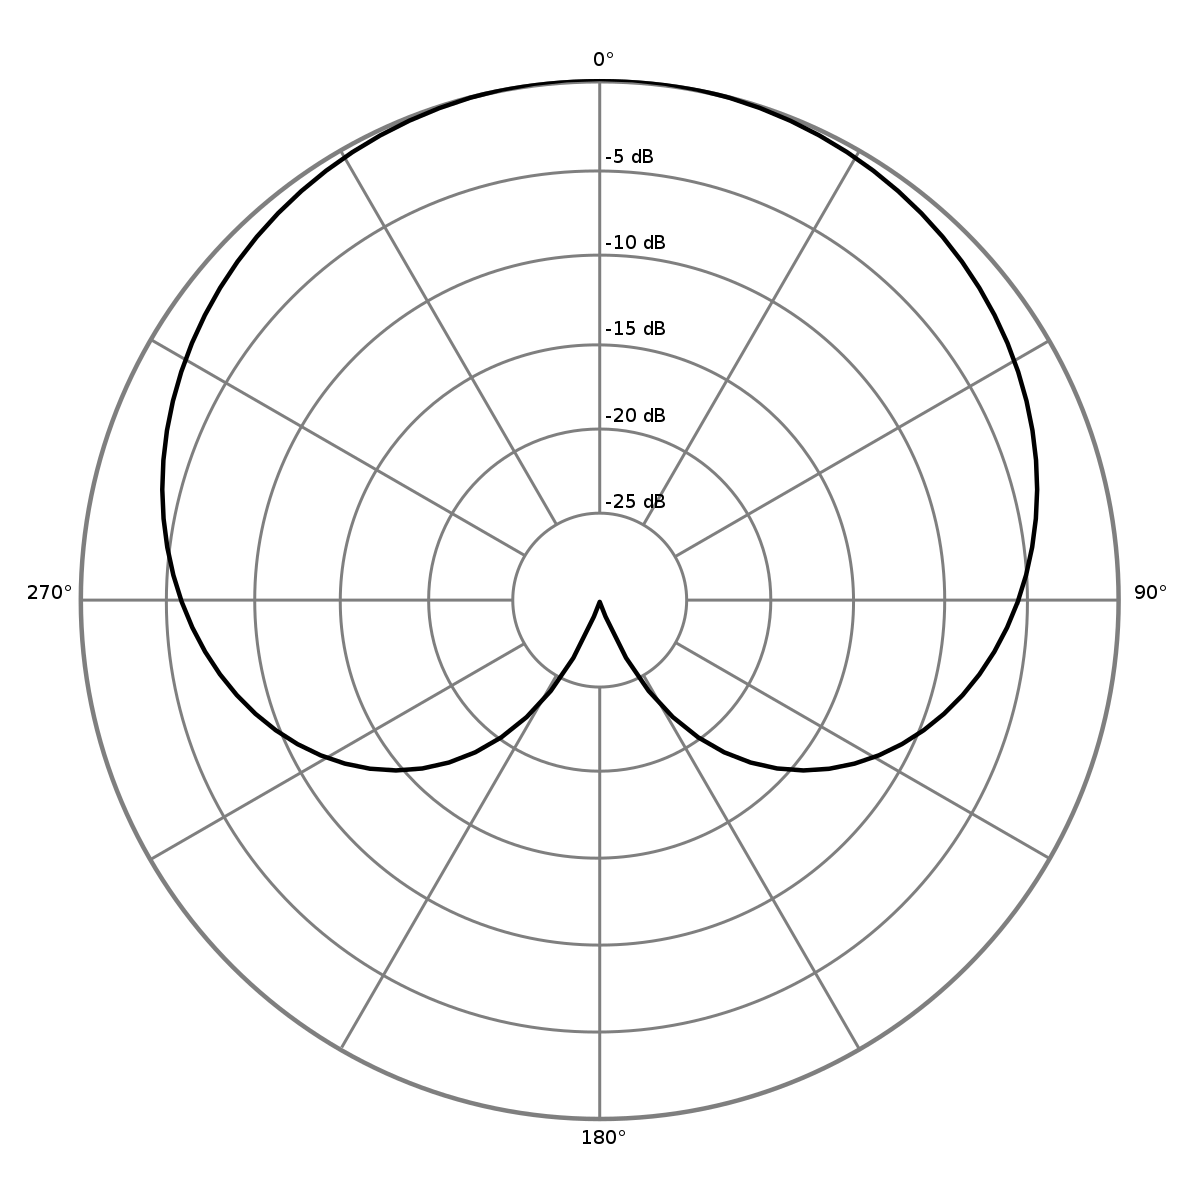
\includegraphics[width=\linewidth]{img/card.png}
  \caption{Cardioid Polar Pattern \cite{card_pic}}\label{fig:card}
\endminipage\hfill
\minipage{0.32\textwidth}
  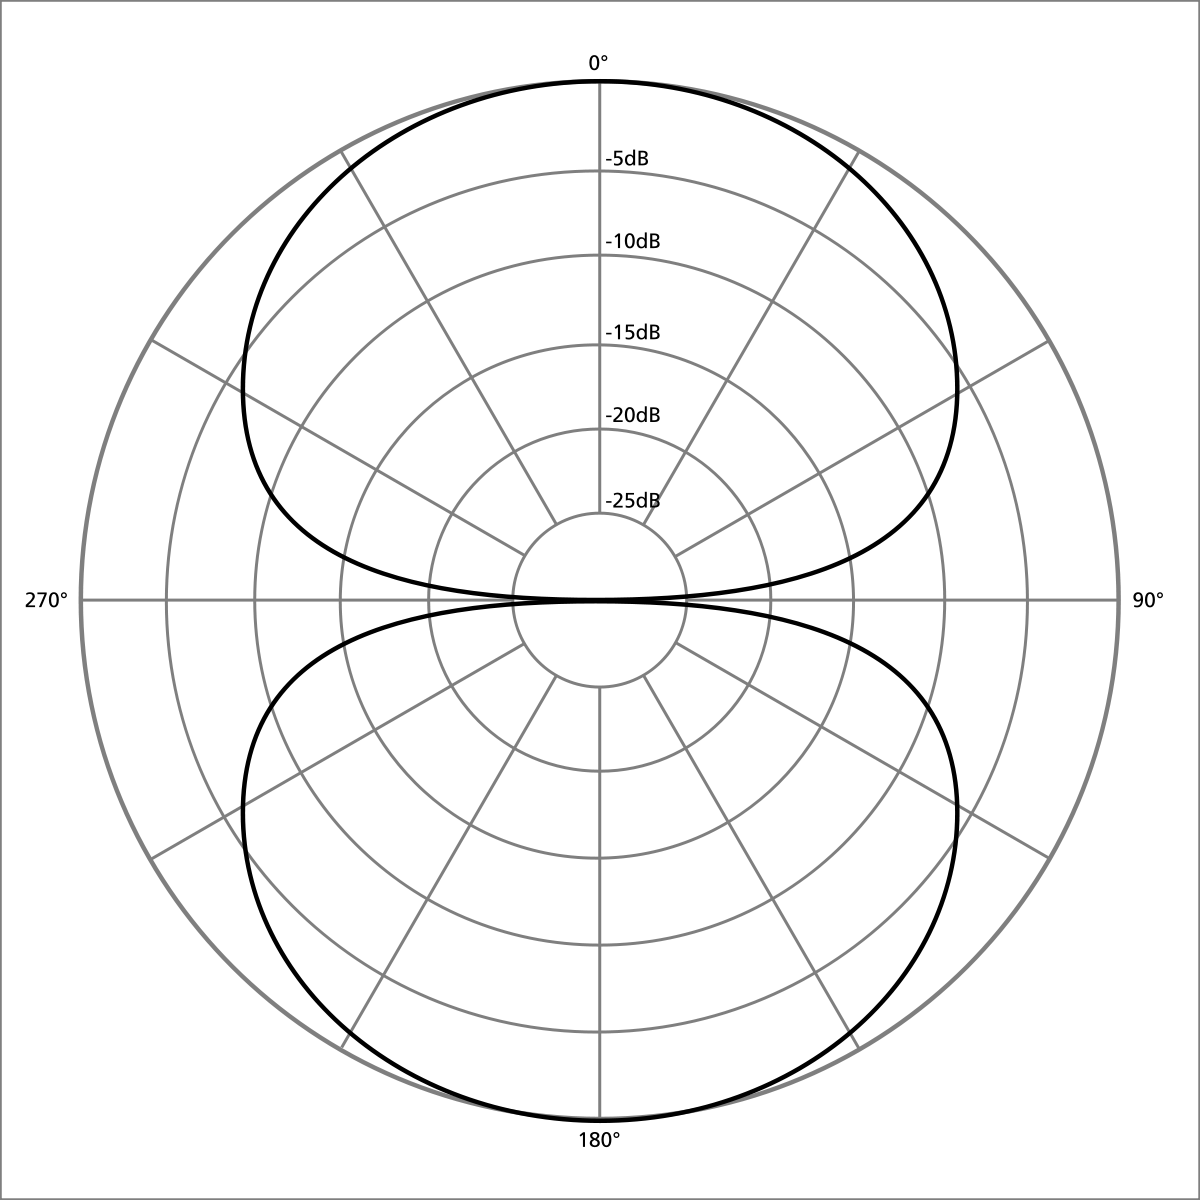
\includegraphics[width=\linewidth]{img/fig-8.png}
  \caption{Figure-8 Polar Pattern \cite{fig8_pic}}\label{fig:fig-8}
\endminipage\hfill
\minipage{0.32\textwidth}%
  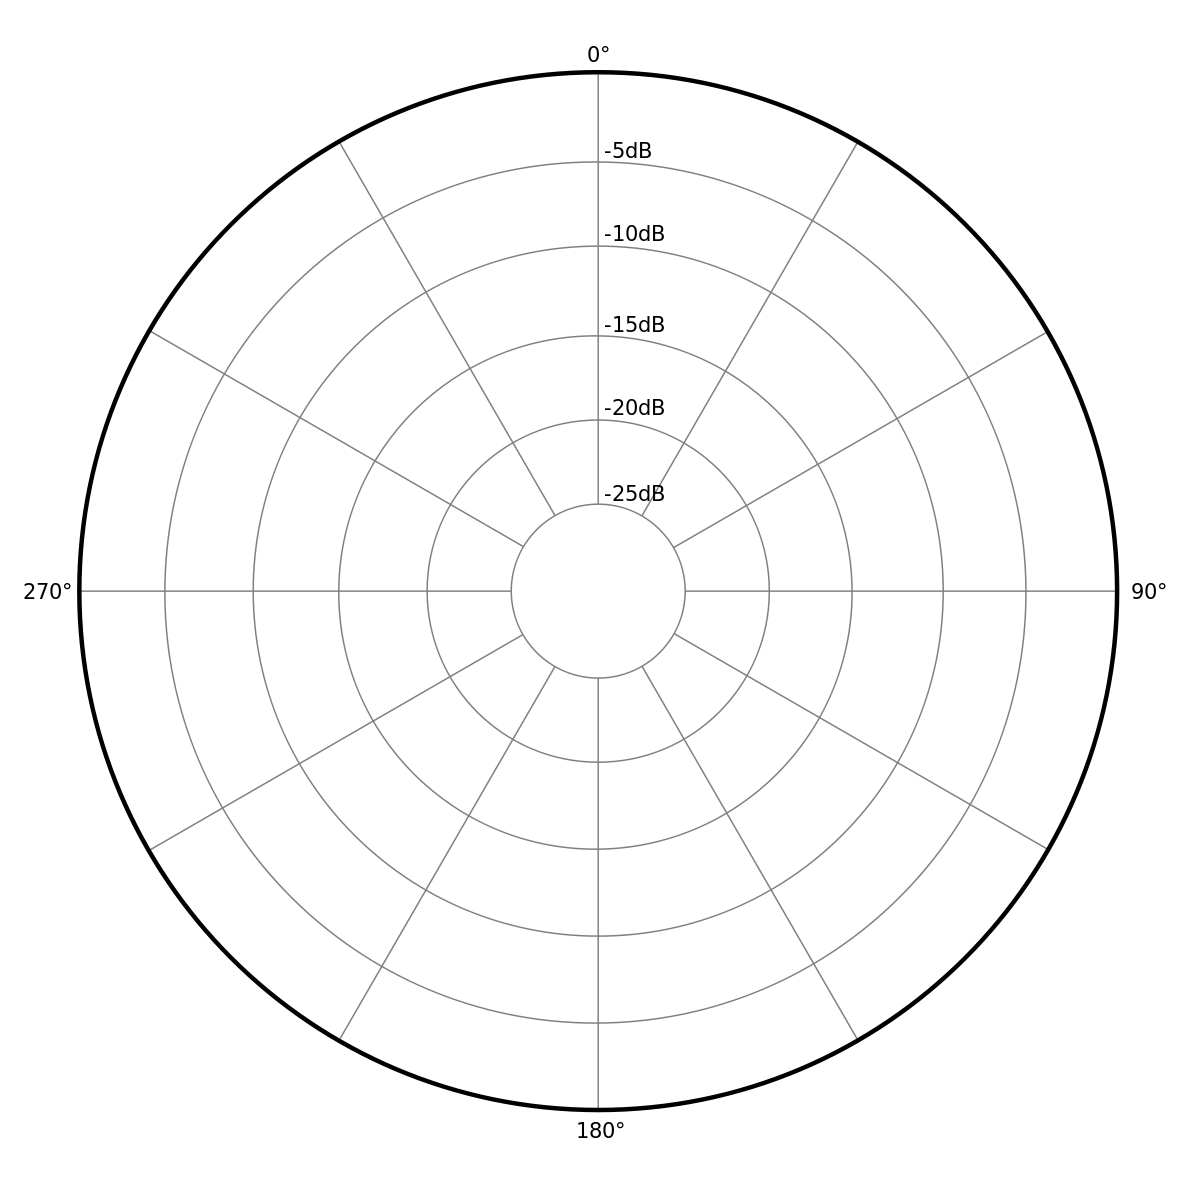
\includegraphics[width=\linewidth]{img/omni.png}
  \caption{Omni Polar Pattern \cite{omni_pic}}\label{fig:omni}
\endminipage
\end{figure}

These idealized responses show the sensitivity of different microphones to sound waves arriving from different directions. For the cardioid\footnote{Which gets it's name from it's heart-shaped response.} pattern, we see a \textit{null} at 180\textdegree and \textit{unity} response at 0\textdegree. These diagrams are seldom true in real-life, especially for high frequencies. Even for very good omni-directional microphones, eventually the capsule size becomes comparable to that of the wavelength, making the response directional. 

\textit{Off-axis coloration} refers to microphone's difference in frequency response at different directions. Most microphones can intuitively be separated into \textit{side address} or \textit{front address} microphones based on their construction. For \textit{front address} microphones, the reported frequency response will likely be based on a measurement with the capsule facing the excitation source so the response matches the ergonomic use of the microphone. Any \textit{side address} microphone, such as a cardioid condenser microphone, would perform poorly if the musician oriented the microphone backwards, resulting in a different frequency response than expected.

\textit{Proximity effect} is another term which relates to the nature of unidirectional microphones\footnote{Cardioids and figure-8 microphones fall under this category.} to exhibit a bass-boost when placed too close to the source. This is why many condenser microphones come equipped with a bass roll-off switch. The bass-boost comes from the \textit{pressure gradient} microphone. At low enough frequencies, the wavelength is vastly larger than the microphone capsule, so the difference in pressure at either side can be unnaturally large. This effect should be considered when placing musicians in relation to the microphones.

The mid-side (MS) technique previously discussed is just one of several stereo techniques that are traditionally implemented for stereo recording. While other stereo techniques such as A/B, X/Y, and ORTF also exist, these fall outside the scope of this text. The reader is referred to \cite{lipshitz1986stereo} for a lively discussion on the merits of coincident and spaced arrays for stereo reproduction. It warrants mentioning that by no means are surround-sound techniques objectively superior. In fact, there is still a lot of research being undertaken in this domain, in particular by The University of Huddersfield \cite{lee3d}. 

\textit{Spaced arrays} are a family of microphone arrays designed originally for surround sound formats. Various authors over the years have experimented and documented their configurations in order to facilitate the creation of high-quality multi-channel music for film. Figure \ref{fig:c-spaced-arrays} shows five complete spaced arrays adapted from \cite{hacihabiboglu2017perceptual} and \cite{politis2016microphone}. The diagram created is a rough approximation of these five 5.1 arrays. In addition to these five arrays, ambisonic arrays are also considered complete \textit{coincident} arrays capable of encoding surround sound formats. \cite{Immersiv9:online} also provides information about these arrays\footnote{Distances and angles might be slightly different from one reference to another. \textbf{TODO}}.

% 5.1 arrays (Fukada Tree, INA-5, Hamasaki Tree, DPA 5100, OCT-surround)
\begin{figure}[ht!]%force figure here, top, strict
\centering
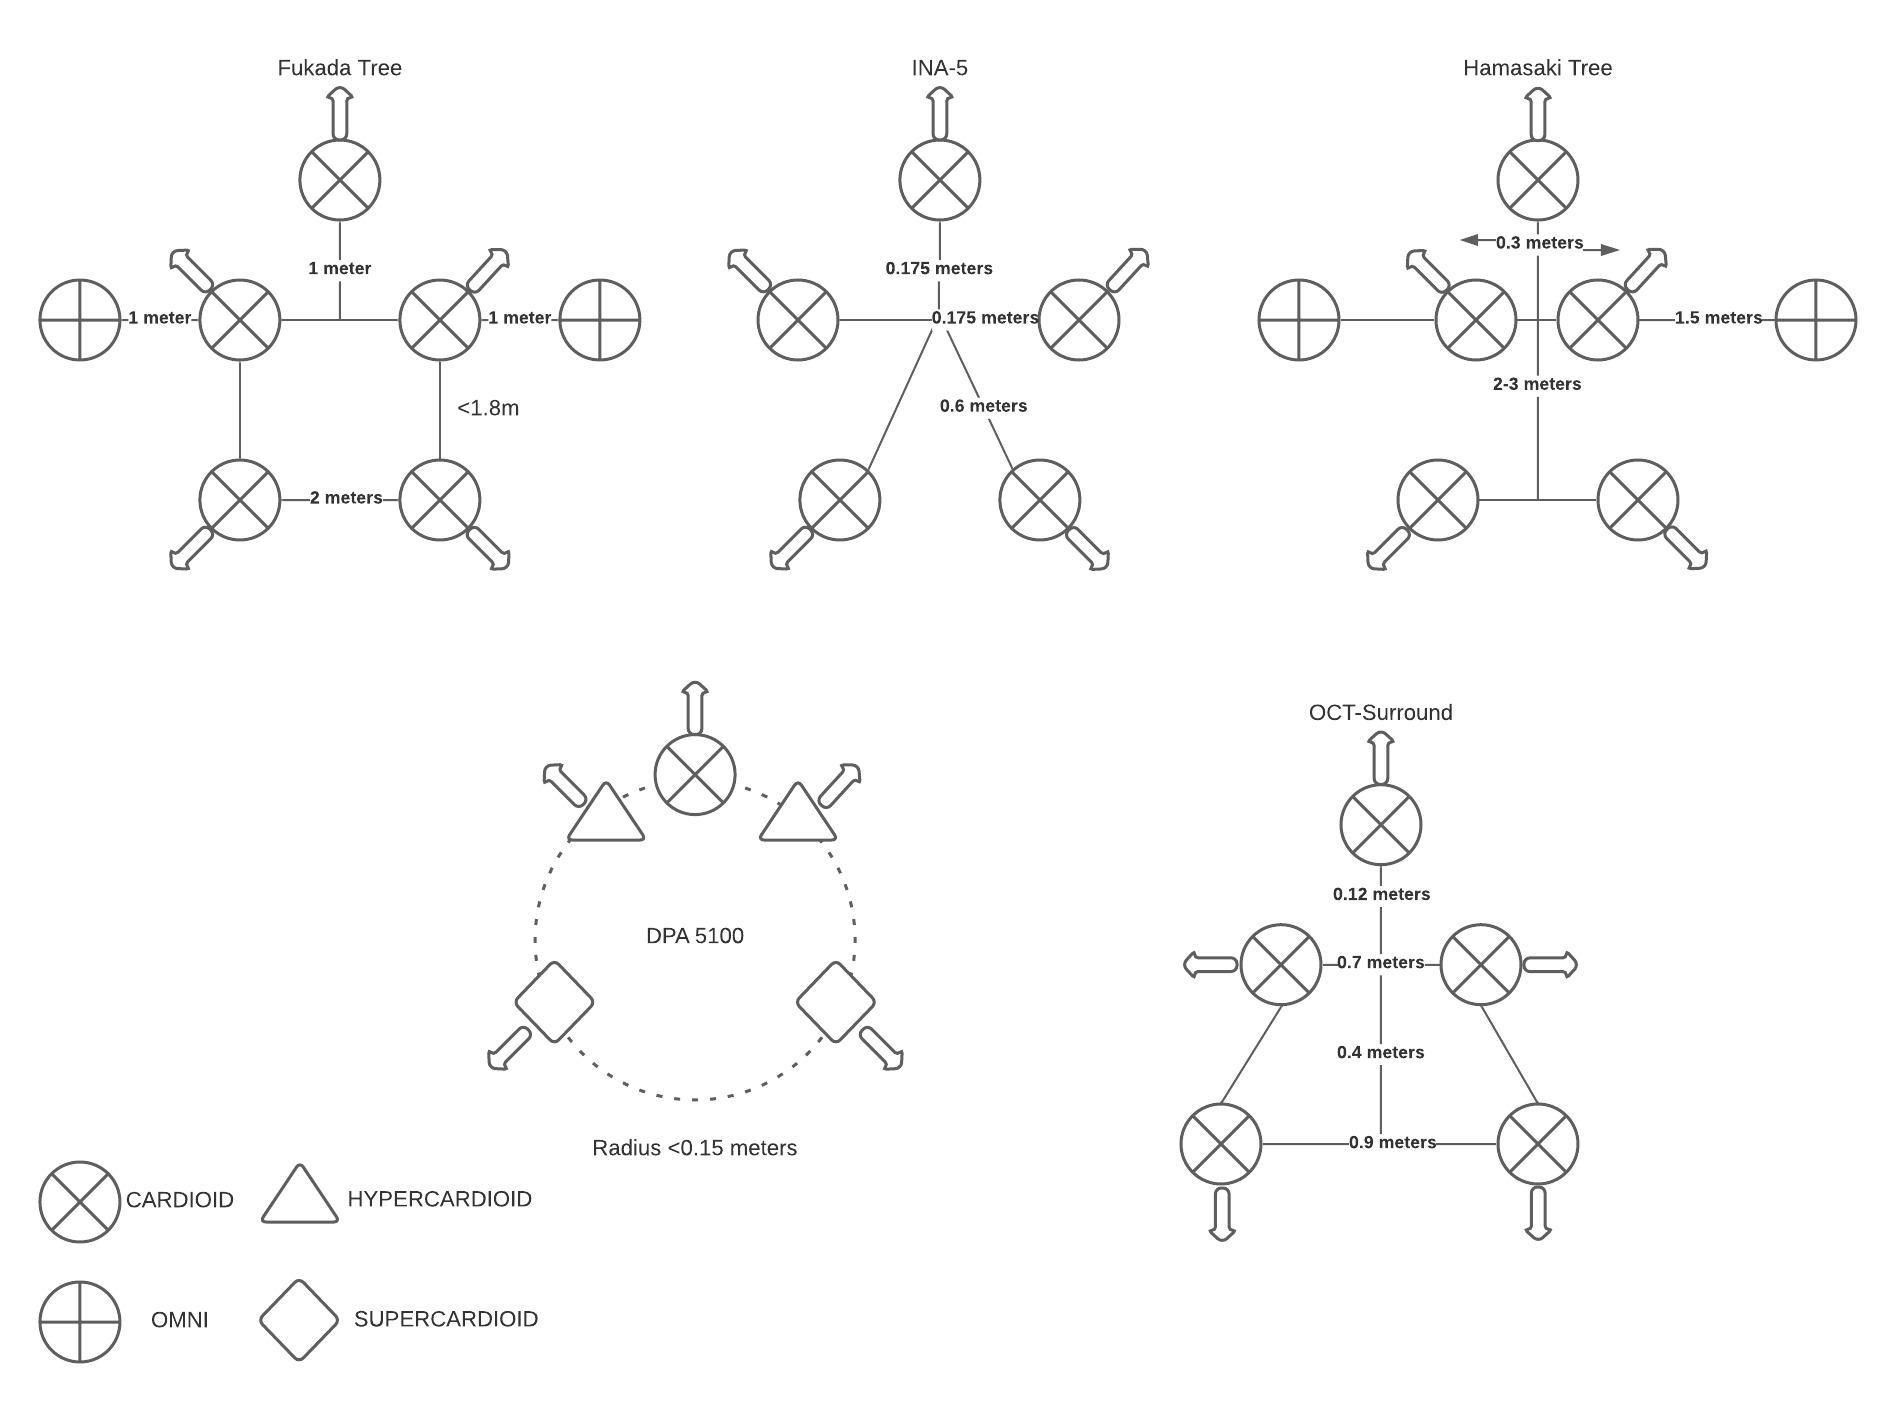
\includegraphics[width=1.0\textwidth]{img/complete-spaced-arrays.jpeg} 
%\captionsetup{justification=centering}
\label{fig:c-spaced-arrays}
\caption{Complete Spaced Arrays}
\end{figure}

\todo[inline]{The symbols I used for these drawings are not standard. Not sure if that is ok.}

In addition to the five depicted arrays:
\begin{enumerate}
    \item \textbf{Fukada Tree}
    \item \textbf{INA-5} 
    \item \textbf{Hamasaki Tree}
    \item \textbf{DPA 5100}
    \item \textbf{OCT-surround}
\end{enumerate}

% Front arrays (Optimal Cardioid Triangle, Decca Tree, INA-3). Rear arrays (Hamasaki Square, IRT Cross)

A secondary technique exists for multi-channel audio recordings which involves a combination of a proximal front array and a distant rear array. In this configuration it is up to the sound engineer to decide how distantly the rear array will be placed. The decision will be based generally on the size of the space as well as how diffuse the sound is at the set distance. Front arrays include: Optimal Cardioid Triangle, Decca Tree, and INA-3. Rear arrays include: Hamasaki Square, and IRT Cross. Figure \ref{fig:fnr-arrays} shows a coarse approximation the associated arrays. The front two receivers in the rear array are summed with the side receivers from the front array in this 5.1 set-up. 

\begin{figure}[ht!]%force figure here, top, strict
\centering
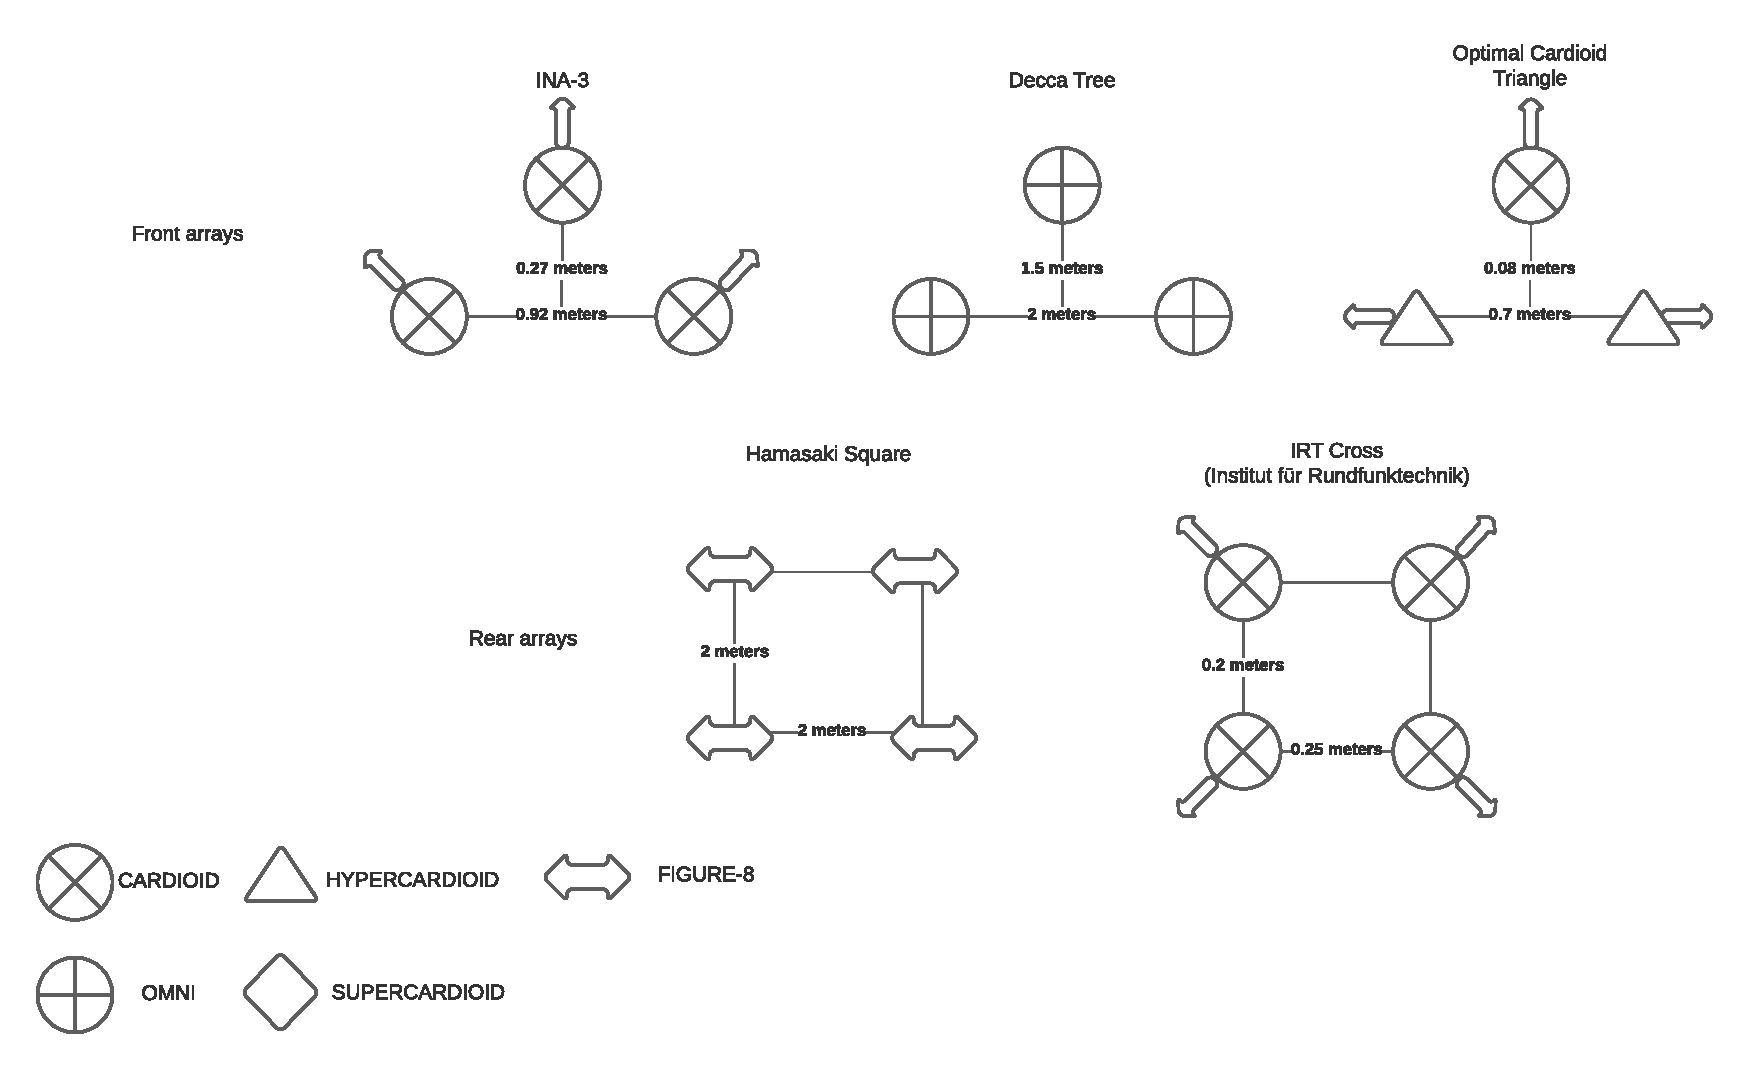
\includegraphics[width=1.0\textwidth]{img/front-n-rear-arrays.pdf} 
%\captionsetup{justification=centering}
\label{fig:fnr-arrays}
\caption{Front and Rear Arrays}
\end{figure}

\subsection{Encoding Monophonic Sources}

% The recording array from the grid mics are numbers 15+17, 18+20, and 27+30. Those mics are mixed in with the hanging ORTF pair, which moves from time to time. So that’s 6 available right now. 

The same principle of ambisonic panning, formerly introduced as a technique for creating spatial representations in music, can be extended as a recording technique for 3D audio scene construction. In this approach, rather than specifying the positions of the desired sound source trajectories, we define for the encoder the positions of the statically placed microphones used for the recording. For example, within our experimental concert hall at CPMC, it is possible to define a template with the location of our fixed microphone locations, used routinely for concert recording. By placing the appropriate channels in the location tracks with the corresponding panners, we can render the recordings in a multi-channel format for playback over headphones or multi-channel speaker systems. Figure \ref{fig:cpmc122-mic-grid} shows the positions of 6 microphones typically used by our house engineers for multi-track recording. An additional ORTF pair located at the center of the grid is also included in the multi-track recordings, however, the position of this pair is not perpetually fixed\footnote{According to our house engineer.}. 

\begin{figure}[h!]%force figure here, top, strict
\centering
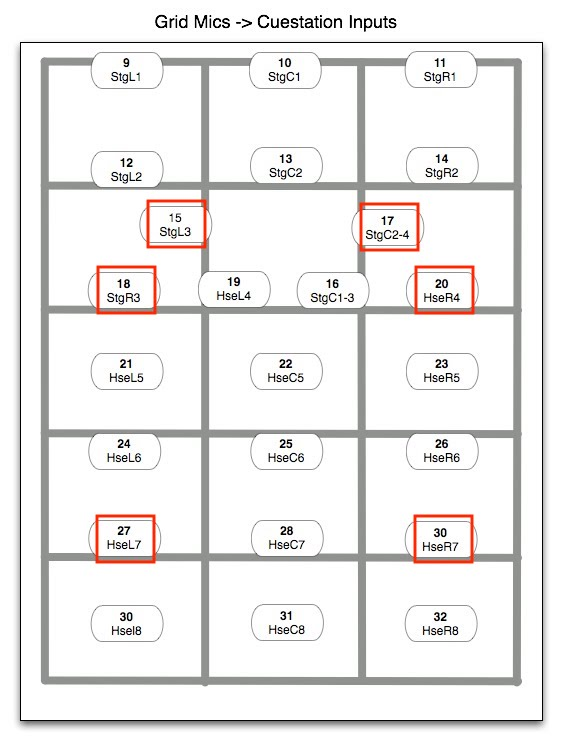
\includegraphics[width=0.5\textwidth]{img/cpmc122-mics.jpg} 
%\captionsetup{justification=centering}
\label{fig:cpmc122-mic-grid}
\caption{CPMC122 Microphone Grid - UCSD Dept. Music}
\end{figure}

A common technique implemented by recording engineers is combining multi-channel microphone arrays with fixed microphones. In the aforementioned case the 6 microphones are distant from our musicians and as a result they pick up sounds from all instruments on stage. In order to isolate sources, giving us more control in post-production, \textit{spot microphones} can be placed closer to the musicians. Ideally, the distances of all these fixed receivers are calculated in relation to the ideal listening position, both in terms of azimuth and elevation. 

\subsection{Coincident Microphone Arrays}

Of primary importance to our work is the development and optimization of coincident microphone arrays. Coincident microphone arrays come in various shape and sizes. The predominant characteristic of these devices is that proximity between sensors is minimized in order to improve localization estimations and the operating frequency \textit{virtual microphones} created by combinations of signals. There are three main types of coincident microphone arrays we were able to discern from the literature: spherical microphone arrays, studio microphone arrays, and planar microphone arrays. While most planar microphone arrays are not meant for high-quality studio recordings, we will nonetheless cover them here since many use similar operational conditions as the proposed HOA system being developed by the author. 
\subsubsection{Planar Microphone Arrays}

Planar microphone arrays are a subset of coincident microphone arrays which attempt to sample a sound-field using either a linear (one-dimensional arrays), or circular array (two-dimensional arrays). Most planar microphone arrays, although not all, fall under tha category of arrays for \textit{noise suppression}, as opposed to studio arrays for multi-channel recording. These devices tend to output a lower number of audio channel that is the sum of various sensors delayed based on the desired direction(s) of sound capture. 

\cite{backman2006miniature} provides some insight into planar microphone arrays and their relationship to sound-field microphones. The author in that publication relies on Micro-Electrical Mechanical Systems (MEMS) capsules for his designs, much like in the authors own work. Backman suggests using multiple transducers to improve signal-to-noise ratio (SNR) and improve polar pattern control over the entire audio bandwidth (20Hz-20kHz). In a second paper \cite{backman2006gradient} the author expanded upon the theoretical work proposing a 5.1 planar array based on MEMS. Unfortunately, little information was presented regarding a 3D audio capture system - the designs described were predominantly for 2D audio. 

\todo[inline]{I want to come back to these Backman papers and add more detail. There are some useful equations there. Unless they are covered more clearly in other papers.}

\cite{chen2015theory} provides a more thorough review of planar arrays. Chen's paper describes a 2D planar array designed with first order microphones which can suitably sample vertical elements of the sound-field. The benefit of planar arrays is that for certain applications, spherical arrays simply might not be possible to construct, such as in cellphone or tablet designs. One noteworthy process implemented in that publication, as well as several others, is the use of simulated responses to validate designs prior to implementation. The main problem we found with this design was the limited bandwidth which had a maximum frequency of 850Hz. For high-quality audio purposes, we seek instead to operate on the audible frequency range. Secondly, in order to sample vertical harmonics, the number of transducers had to be increased from nine, the minimum number required for 2OA\footnote{Second order ambisonics.}, to 16, which increases the cost of the final design. 

Meyer and Elko of \textit{mh acoustics}, the company responsible for the em32 Eigenmike\footnote{https://mhacoustics.com/}, described a second order augmented circular microphone in a 2008 publication \cite{meyer2008spherical}. In their paper, Meyer et al. described using a single central sensor to provide vertical control of the desired \textit{beam-pattern}. The beam-patterns are controlled by adjusting the weights in the linear combination of spatial harmonic signals (also referred to as \textit{eigenbeams} or \textit{eigenmodes}). Their design has 7 capsules "flush mounted into the top surface of a puck-like housing". There are 6 capsules along the diameter of the puck, with a radius of 3cm, along with one central capsule. This design seems suitably promising for play-back over dome-like loudspeaker systems since very few sound systems around the world have below-listener speakers. However, the design might be unsatisfactory for applications which use binaural synthesis featuring HRTFs below the listeners' ear level, since that part of the sound-field would not be properly reconstructed. Two other details stand out about the design:

\begin{enumerate}
    \item The microphones are described as pointing upwards rather than outwards. Mounting them on the side of the puck would have likely improved the performance of the array. 
    \item The author's never specify what capsules are used and there is little information regarding how to recreate the experiment.
\end{enumerate}

There are also two metrics mentioned by Meyer et al. we should discuss Directivity Index (DI) and White Noise Gain (WNG). The DI is the difference in \textit{decibels} between the sound pressure level (SPL) in a given direction and the average SPL from an omni-directional source \cite{LONG201439}:

$$
\mathrm{D}(\theta, \phi)=\mathrm{L}_{\mathrm{p}}(\theta, \phi)-\overline{\mathrm{L}}_{\mathrm{p}}
$$
where \\
    $\mathrm{D}(\theta, \phi)=$ directivity index $($ gain $)$ for a given direction $(\mathrm{dB})$ \\
    $\mathrm{L}_{\mathrm{p}}(\theta, \phi)=$ sound pressure level for a given direction $(\mathrm{dB})$ \\
    $\overline{\mathrm{L}}_{\mathrm{p}}=$ sound pressure level averaged over all angels $(\mathrm{dB})$ \\
    $(\theta, \phi)=$ some specified direction.

\todo[inline]{Make sure you are consistent with phi and theta in your code.}

WNG is a quality metric of beamforming algorithms. It is defined as the beaformer's ability to suppress spatialy uncorrelated noise. Note that self-noise and external white noise may be statistically indistinguishable, so WNG constraints should consider self-noise as well. Mismatch between sensor characteristics and position errors can also result in spatially white noise \cite{mabande2009design}.  

\todo[inline]{middlicott 5 channel array, ambi, circular}

% According to the authors, directional microphones, are less well-matched than omni-directional microphones. Matching capsules is important for good sound-field sampling. 

% As the author suggests, most authors today are less interested in horizontal only audio capture, and even less so in systems which only sample the sound-field in 1D - likely because surround sound has encouraged the creation of material with 2D qualities. Extending WFS to a 2D representation yields a similar representation to that generated by VBAP \cite{smith2019spatial}. 
% Planar microphone arrays have nonetheless become increasingly popular as systems for direction-of-arrival (DOA) estimation and subsequent beamforming operations. In these systems, the linear microphone array is used to estimate the DOA of a signal using statistical analysis of the signals. Then, a beamforing operation can be performed on these same signals to generate a highly directive microphone pattern \textit{pointing} at specified location. This can be used, for example, to isolate and improve the quality of recording for a speaking person within a noisy environment. The same principle has also been applied to circular and spherical arrays. 

\subsubsection{Spherical Microphone Arrays}

Spherical microphone arrays are particularly interesting to us because they represent a simple way of capturing spatial sound both in a studio setting and in nature. In contrast to other recording techniques in which musician coordinates need to be defined in order to create a adequate sound-field, spherical microphone arrays inherently encode this information into what are called A-format recordings which are then encoded into the spherical domain for reproduction over an arbitrary loudspeaker or binaural system. 

Spherical microphone arrays can further be separated into three types of arrays: rigid, hollow, and tiered. Tiered arrays constitute arrays in which various radii are superimposed in order to capture different regions of interest of the sound-field (cite). In general, these systems have gotten less attention due to the difficulty of integrating these models with camera systems. Rigid and hollow models are more popular, and corresponding mathematical formulations exist for both. At their names suggest, a rigid spherical microphone array has no cavities exposed to the outside of the array, while the hollow designs do have open spaces over which sound may propagate.

In general, it rigid microphone arrays have gotten the most attention from the commercial sector, because of the elegance of their complimentary design with multi-camera systems, however, hollow arrays have also been implemented commercially in audio-only designs, targeted towards audio engineers who are not interested in producing video content. 

\subsubsection{Studio Microphone Arrays}
%This section describes some studio coincident microphone arrays. 
These are all studio techniques in which microphones are placed as close together as physically possible. 

Native B-format array, double MS, double MSZ, etc.

\subsection{Arrays in series}
A modern type of sound capture technique has recently been developed and is the subject of great interest for spatial audio researchers. The technique, predominantly employed under the basis of ambisonic rendering, involves capturing multiple sound-fields simulateneously using an \textit{array of arrays}. In other words, a recording engineer positions a grid of multiple spaced microphone arrays in such a way that the \textit{acoustic boundaries} of adjacent arrays overlap each other. 

The goal of this capture technique is to allow, within a digital representation, six degrees of freedom (6DoF), or, \textit{translational} movement, in addition to the standard rotational control. Figure \ref{fig:6DoF} shows these translational transformations where yaw, pitch, and roll correspond to rotational transformations. 

\begin{figure}[h!]%force figure here, top, strict
\centering
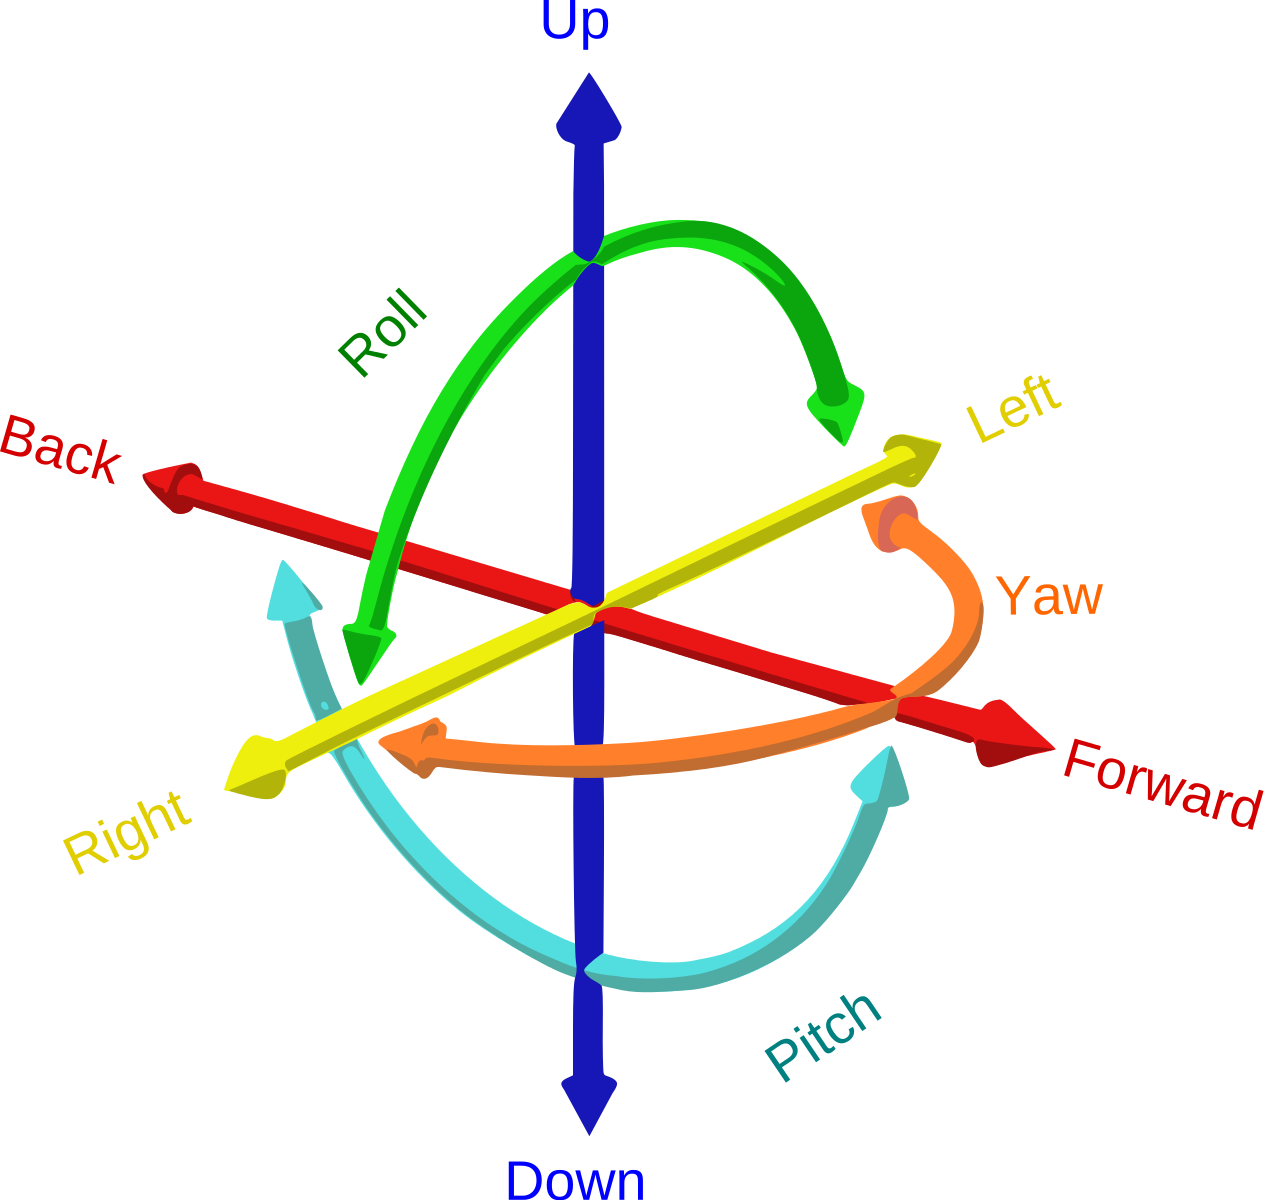
\includegraphics[width=0.5\textwidth]{img/6DOF.svg.png} 
%\captionsetup{justification=centering}
\label{fig:6DoF}
\caption{6DoF - wikimedia commons}
\end{figure}

\section{Open Tools for Spatial Audio Capture}

\todo[inline]{what about video editors? Blender? DaVinci Resolve? }

A number of authors have described the development of Free and Open Source Hardware (FOSH) for the capture of real sound-fields for either asynchronous or synchronous transmission. The majority of these designs fall under the category of spherical microphone arrays although other projects exist which discuss alternative geometries for spatial audio capture. While many publications have been presented wherein the authors describe the creation of such systems, few have actually sought to provide full documentation detailing the process undertaken to realize the entire system. 

A common problem with these designs for musicians seeking to enter the world of sound-field recording is the costly price-point of some of the Bills of Materials (BoMs) suggested by the engineers. In order to swap parts, the musician would need to know about electronics specifications and how to modify Computer Assisted Design (CAD) files in order to create his or her own systems.

\section{Contemporary Spatial Audio Reproduction Techniques} \label{sec:contemp_audio_reproduction}

In the previous section we talked extensively about the artists and engineers who have shaped the way we think and talk about spatial sound. The various sections to follow will provide a look into some of the state-of-the-art research regarding spatial audio solutions and the: composers, institutions and practices, which are pushing us to further our understanding and curiosity. 

\subsection{Amplitude Panners}
\label{subsec:amplitude panner}

\todo[inline]{VBAP, DBAP, other panners, octo, quad, etc. kapralos-2008-virtual-aud-sys-mit.pdf see 4.2.2 amplitude panning. Zirkonium. }

Out of the various iterations of vector based systems the most prominent and well-regarded is called Vector Based Amplitude Panning (VBAP). In his 2001 paper (citation) Pulkii describes how trigonometric operations can be used to position a sound in any position in 3D space. The idea behind VBAP is to create \textit{phantom images} between sources giving listeners the illusion that sounds emanate from any arbitrary position between 2 or more speakers. Pulkii, the inventor of VBAP, from Helsinki, Finland, writes in regards to the difference between this method and ambisonic panning\footnote{Ambisonic panning does not use spherical microphones but encodes arbitrary audio sources for ambisonic reproduction.}: "the gain factor calculation in the VBAP method equals that of the Ambisonics in an orthogonal\footnote{Regular loudspeaker layouts.} loudspeaker placement". The key difference is that VBAP generalizes the calculation for all situations making it extremely flexible. While these two systems might seem remarkably similar, experiments have suggested that there exist statistically significant perceptual differences for both reproduction methods (Marentakis 2014). VBAP has gained much popularity among composers due to it's simplicity and elegance. A MAX/MSP collection of externals were developed by Pulkii in 2000 to allow electronic musicians to experiment with the system making it fairly accessible. It should be noted that as with many other spatialization methods it relies heavily on a great number of speakers for successful immersion. 

% \subsection{Modeling}
% \subsubsection{Wave-Based Modeling}

% Wave-based modeling involves solving the wave equation, also known as the \textit{Helmholtz-Kirchoff} equation, to create a Room Impulse Response (RIR) that models a particular sound-field. 

\subsection{Object Based Audio}
\label{subsec:oba}

Object Based Audio (OBA) is a format agnostic method, much like ambisonics, in which audio objects carry metadata which are used by the \textit{renderer} to successfully reproduce each sound source \cite{coleman2018audio}. Some of the parameters included in the metadata of each audio object include: level, position, radius, and spread\cite{fug2014design}. In contrast to ambisonics, in which the sound-field might be pre-rendered, OBA requires real-time rendering of objects within a scene. The benefit of this method is that the listener gains control of the "mix". Using OBA the listener can, for example, adjust the balance between dialog and background sounds - a feature which highly desirable since a preponderance of background sounds can sometimes reduce speech intelligibility beyond comprehension. There are several software platforms which support OBA, here we will only cover a few and focus particularly on systems related to computer-music.

Among the various technologies used to create OBA, the MPEG-H\footnote{The Moving Picture Experts Group (MPEG) is an alliance of working groups of ISO (International Organization for Standardization) and IEC (International Electrotechnical Commission) that sets standards for media coding, including compression coding of audio, video, graphics and genomic data, and transmission and file formats for various applications.} CODEC (COder/DECoder) has become the most popular in commercial settings. Herre describes OBA in \cite{herre2015mpeg}:

\begin{quote}
    More recently, the merits of object-based representation of a sound scene have been embraced by sound producers, e.g. to convey sound effects like the fly-over of a plane or space ship. Audio objects are signals that are to be reproduced as to originate from a specific target location that is specified by associated side information. In contrast to channel signals, the actual placement of audio objects can vary over time and is not necessarily pre-defined during the sound production process but by rendering it to the target loudspeaker setup at the time of reproduction. This may also include user interactivity.
\end{quote}

VBAP and OBA are closely related as reproduction methods. In fact, OBA typically uses VBAP in order to render the sound objects. In addition, the MPEG-H framework also includes the possibility of streaming HOA and discrete channels data (typically used in surround sound formats) in order to synthesize a hybrid format. In addition to this, the standard counts with a consistent perceptually motivated compression system used to lower the amount of data required for accurate spatial reproduction. One can sign-up to receive some authoring software for MPEG-H via the  \href{https://www.iis.fraunhofer.de/en/ff/amm/dl/software/mas.html}{Fraunhofer website}. Some other projects have embraced the Opus CODEC for compression in streaming solutions requiring spatial audio\footnote{One such project is \href{Earshot}{https://github.com/EnvelopSound/Earshot} by Envelop.}.

Recently the Groupe de Recherche en Immersion Spatiale (GRIS) at Université de Montréal published a self-proclaimed OBA authoring system called \textit{SpatGRIS/ServerGRIS}. Previously, SpatGRIS was used in conjunction with the Zirkonium software\footnote{https://zkm.de/en/about-the-zkm/organization/hertz-lab/software/zirkonium} from ZKM. Today, ServerGRIS serves as a standalone spatialization system which can be used in conjunction with ServerGRIS to spatialize sounds in dome-like environments via VBAP. SpatGRIS has two modes, one in which it performs the spatialization itself, and one in which it sends OSC data to ServerGRIS. SpatGRIS also works with DAWs which route audio via JackRouter to ServerGRIS to perform the gain adjustments. In this sense, one can consider the GRIS system as an OBA format, since each audio channel has an associated data track defining its spatial properties.

The software's user interface makes used of \href{https://en.wikipedia.org/wiki/Cocoa_(API)}{Cocoa} which makes it compatible only with OSx\footnote{NOT COMPATIBLE WITH CATALINA (10.15) - Jan 29, 2021}. The benefit of SpatGRIS/ServerGRIS over VBAP inside Pd is that the software provides a binaural renderer which allows the user to audition their multi-channel work preemptively. Unfortunately, there does not seem to be a way to dynamically rotate the sound-field as with HOA, so the binaural rendering will be static. The software is also more dynamic than the Pd VBAP system with regards to re-routing of audio signals in different environments, and, automating trajectories in a DAW is far more comfortable than doing so in Pd, which requires the user specifying coordinates using a text editor. 

Ledoux, one of the authors of the GRIS software, describes the benefits of OBA:

\begin{quote}
    This object-based audio approach has the advantage of dissociating sound source’s localisation from the loudspeakers position and allows pre-spatialized music to be portable from one dome to another, regardless of the amount of loudspeakers and their relative position. \cite{ledoux2018immersive}
\end{quote}

In addition to the MPEG-H standard, there is also Dolby Atmos and DTS:X. Both companies have a long tradition of driving the market and have proposed standards for multi-channel film production over the years. Mac and Pc version of the Dolby software can be found \href{https://developer.dolby.com/tools-media/production-tools/dolby-atmos-mastering-suite-updates/downloads/#!}{here}. The DTS-X creator suite can be purchased \href{https://dts.com/production-tools/#creator-suite}{here}. DTS-X also counts with a video player which can playback ambisonics, the reader is referred to \href{https://www.videolan.org/vlc/releases/3.0.0.html}{VLC} for a FOSS solution. 

One final project that might interesting to the reader is SpatDIF which is short for Spatial Sound Description Interchange Format \cite{peters2012spatdif}. The project as it stands is mostly defunct now but the Pd externals can still be \href{https://www.zhdk.ch/en/research/icst}{found online} at the ICST website from ZHDK\footnote{Zürcher Hochschule der Künste or "Zurich University of the Arts". Zurich is the largest city in Switzerland.}. The SpatDIF project is now integrated into the ZKM\footnote{ZKM Center for Art and Media Karlsruhe is in Germany.} \href{https://zkm.de/en/about-the-zkm/organization/hertz-lab/software/zirkonium}{Zirkonium} software. 

The Zirkonium software is actually built with Pd but the GUI is only OSx compatible. SpatDIF aimed to store the trajectories of sound objects as XML files that could be read by Pd in real-time. The user could use VBAP or Ambisonics to render the sound objects in their scene. It should be noted that SpatDIF never explicitly calls itself an OBA system, but we believe it could still be categorized as such because each sound has an associated scene description which is used by a renderer at a later stage for reproduction in an arbitrary loudspeaker layout. 

One of the main drawbacks we should point out with OBA is that the number of sound sources will change the number of channels to the stored. This will also be a consideration at the rendering stage. The larger the number of sources, the more computationally expensive it will be to render the sources in real-time. In contrast, ambisonic allows us to represent an arbitrarily large number of sound sources in a limited number of channels with varying quality based on the ambisonic order \cite{scaini2020wavelet}. Scaini provides another definition of OBA in his recently published thesis on wavelet-based spatial-audio framework\footnote{Based on spherical wavelets.}: 

\begin{quote}
    In object based formats the role of encoding and decoding is essentially reversed with respect to the channel based formats. There is no spatial encoding, and the task of generating the gains for each speaker is given to the decoding stage, where a panning law is used at playback time to convert the object metadata into gains. Here the panning law does not define the format, and it is possible to use different panning laws for the same object based format, providing that the panning law ‘understands’ the object metadata.
\end{quote}

\todo[inline]{soundscape renderer?}

%https://github.com/mgeier/spatdifrenderer
%https://sourceforge.net/projects/omprisma/

\subsection{Wave Field Synthesis}
\label{subsec:wfs}

%https://github.com/GameOfLife/WFSCollider

Whilst less commonly seen or talked about, wave field synthesis (WFS) is another area of interest for acousticians and composers. WFS attempts to capture a wavefront and reproduce it at a later stage. A good case scenario for this is the simulation of a live concert. A wall of microphones is placed ten meters from the band and, at a later point, a wall of speakers is used to play back the recorded audio. A new audience could in theory listen to this reproduction and be transported to the event. The audience members could even walk around the "dance floor" and experience the rich spatial detail as if they were really there. WFS is a powerful spatial technique but entirely context dependent. It is often not desirable for situations in which sound arriving from all directions need to be captured. WFS also costly, as proper capture and reproduction takes dozens of microphones and speakers, making it inaccessible for most consumers.

\subsection{Higher Order Ambisonics}
\label{subsec:ambi}

Ambisonics is a full-sphere capture and reproduction method popular among spatial audio enthusiasts. A resurgence in interest, as with any of the aforementioned methods, can be attributed to the growth of mixed reality\footnote{MR: augmented reality in which digital objects can be interacted with}, augmented reality (AR) and virtual reality (VR) systems. Ambisonic has become of the de facto spatial audio reproduction methods in simple VR experiences, especially 360 video. 

Ambisonic signals can be created by panning traditional monophonic recordings or by capturing them via an ambisonic microphone. A tetrahedral microphone, the simplest ambisonic microphone, captures First Order Ambisonic (FOA) A-format\footnote{A-format audio is ambisonic audio prior to encoding.} signals which can be used to reproduce 360 degrees of spatial audio with tolerable quality. 

The theory and application of ambisonic heavily relies of the assumption that the playback system is composed of a spherical array of speakers which situates the listener at the origin. The tetrahedron shape is the lowest geometric approximation of a sphere, its shape is thus chosen for first order ambisonic capture. Higher approximations result in a higher number of channels and better spatial quality at the cost of more data to be handled and stored. The assembly and calibration of Higher Order Ambisonic (HOA) microphones remains a laborious and often HOA panning is used instead.

One of the major limitations of ambisonics recordings captured with these microphones, over other techniques - such as OBA - is the fact that the listener is confined to the geometric position in which the recording was taken in or synthesized for. In VR, AR and MR, users generally are not satisfied with being stationary - even if they can turn and tilt their head. These recordings work suitably well for viewers experiencing 360 videos, but if users want to traverse a digital playground, they will not be able to do so convincingly. It could therefore be said that whilst ambisonic can provide a good ambience layer for these experiences, it relies heavily on other strategies for full immersive experiences. Recent research efforts have focused on the interpolation \textit{between} sound-fields, such that users can move around freely between various ambisonic recordings taken in proximity to each other. 

\subsubsection{Mathematical Formulation}

\subsubsection{Decoding Strategies}

\todo[inline]{beam forming}

\subsection{Binaural Synthesis}
\label{subsec:bin-synth}

\cite{cuevas20193d} provides an extensive literature review on the subject of \textit{binaural spatialization}. In this particular text by Cuevas, one of the most comprehensive writings on binaural synthesis, the authors describe the steps undertaken for each part of the signal chain. Figure \ref{fig:3dti-chain} shows a diagram of the implementation. 

For the \textit{free-field} modeling, an anechoic system based on BIRs/HRIRs is implemented, following:

\todo[inline]{barycentric interpolation?}

\begin{enumerate}
    \item Distance-dependent attenuation (inverse square law or acoustic power law), this step also includes far-field distance simulation modeling air impedance (distance-dependent low-pass filtering).
    \item HRIR obtained using \textit{barycentric interpolation} and are ITDs removed to dynamically adjust for different head sizes.
    \item HRIR convolution.
    \item ITD is computed and added to the signals.
    \item ILD correction for \textit{near-field} sources.
    \item Directional features for hearing aids added(if any).
\end{enumerate}

For the \textit{diffuse-field} modeling, a non-anechoic system based on BRIRs\footnote{Note that BRIRs are not taken in free-field, so these contain reflections.} is implemented as follows:

\begin{enumerate}
    \item Independent distance-dependent attenuation to control the \textit{direct-to-reverberant ratio} (DRR). 
    \item Sources are encoded into 1st Order Ambisonic (FOA).
    \item These channels are convolved with encoded versions of the BRIRs, which have been processed to remove any direct sound.
\end{enumerate}

\begin{figure}[ht!]%force figure here, top, strict
\centering
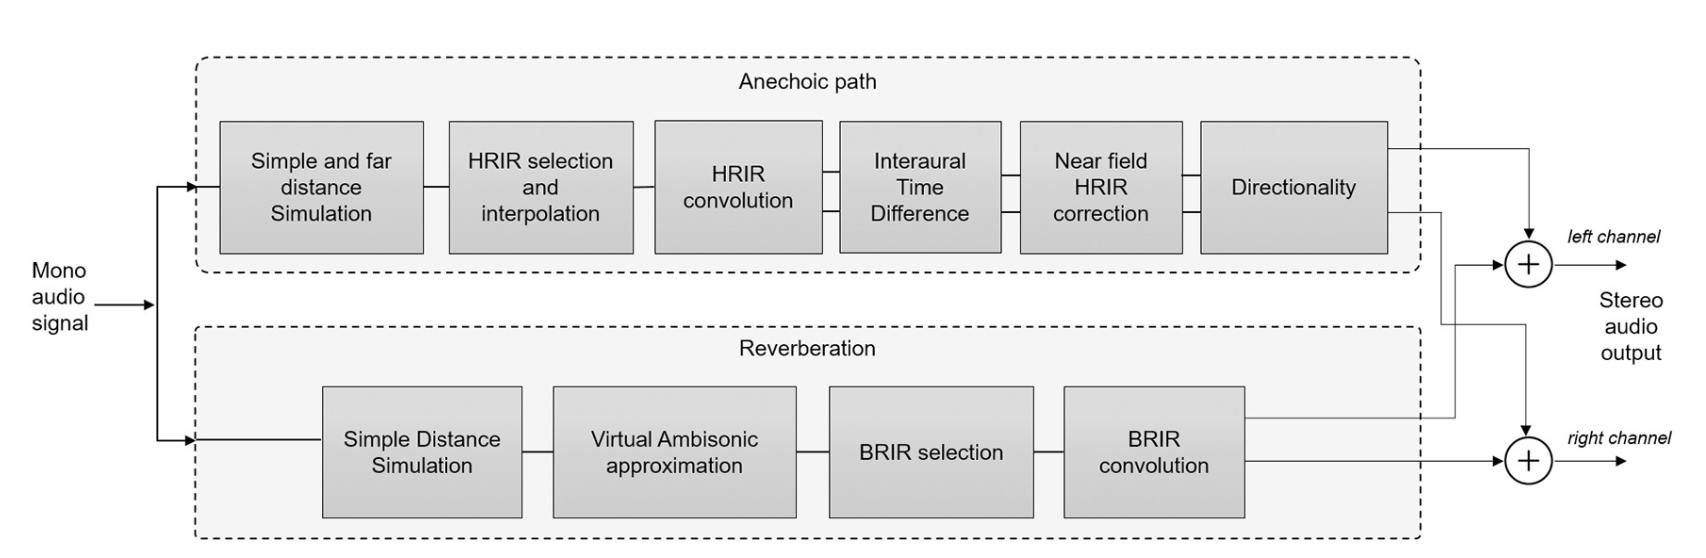
\includegraphics[width=1.0\textwidth]{img/3dti-chain.png} 
%\captionsetup{justification=centering}
\caption{3DTI Toolkit Binaural Structure \cite{cuevas20193d}}
\label{fig:3dti-chain}
\end{figure}

% \subsection{Spherical Speaker Arrays}

\section{Open Tools for Spatial Audio Reproduction}

\todo[inline]{DAWs and VSTs, not CPU mus languages. video players VLC.}

\cite{nettingsmeier2008ambi} provides us with a good description of the processes required to adequately set up an ambisonic playback system at home. We are interested in these particular solution not just because of the robustness of the method, but also because it was designed using all open source software. The benefit of open source software is that it is generally free, and, as a result, it lowers the overall cost of having to mount systems such as the one described. Naturally, a system like this one would still remain far more prohibitive than ambisonics over binaural synthesis within a WebVR experience - for example - but the comparison is really like comparing apples to oranges, WebVR, or any other commercial VR solution, is far from being able to achieve complete multi-modal\footnote{By multi-modal we mean: stimulating more than one sense. "Ideally" the experience would trick all five senses.} immersion.

In the aforementioned publication the author employs a hexagonal horizontal-only speaker set-up, however, it should be noted, the biggest benefit of ambisonics in the context of creating spatial music is the proliferation of binaural decoders for the method which allow one to forego speaker systems entirely\footnote{The quality of the final mix will be dependent on the quality of the binaural decoder.}. What this means is that if a composer is interested in creating music for HDLAs, they need not have access to a sophisticated loudspeaker system - they only need a pair of headphones and computer. In certain contexts, however, it is useful to have multi-channel systems operational and calibrated (for a spatial music class, for example). 

In such a case, where a "real" loudspeaker set-up is required Nettingsmeier, provides us with a good description of the associated steps required to calibrate such a system. Summarily, the steps in that paper are:

\begin{enumerate}
    \item Get all the gear you need, checking that: drivers for interfaces are supported by OS\footnote{You will need a decent amount of RAM. The higher order ambisonics the more RAM will be needed.}.
    \item Organize the number of speakers you have available in the desired layout (in his case a hexagon). 
    \item Measure the distances and angles from the center position and adjust speakers so the vertices of the ideal polygon (or polyhedron) match the mathematical model.  
    \item With the measured angles and distances, create a decoder using the AmbDec by Fons Adriansen\footnote{For Linux only. See ambi-X, IEM Plug-in Suite, or ATK for other systems.}.
    \item Use Aliki and Digital Room Correction (DRC) software to create six correction filters\footnote{This requires a good quality omni mic, such as the umik-1 by miniDSP (used in our work). Alternatively one can borrow a Earthworks M30, or similar measurement microphone from their University.}.
    \item Use an RMS meter to "level match" all your speakers. For this step and the last the center of the "rig" should be the reference point. 
    \item Listen and modify based on your preference. You can change your mind and build a new decoder, or remove speakers if you want. 
\end{enumerate}

\begin{figure}[ht]%force figure here, loosely
\centering
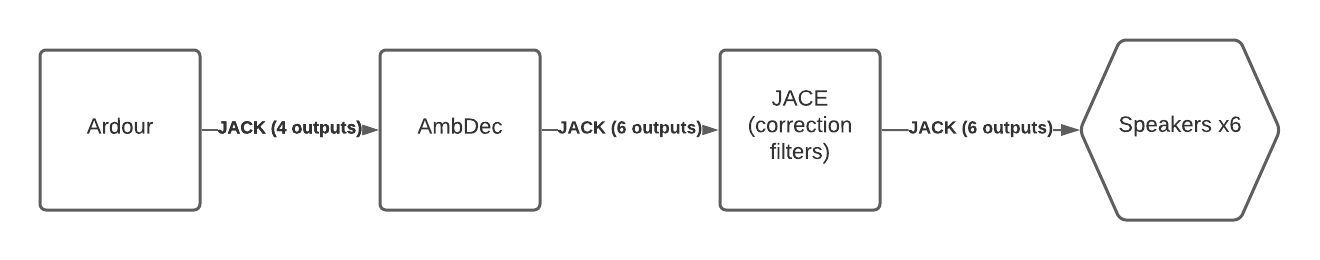
\includegraphics[width=1.0\textwidth]{img/nettingsmeier-extra-frontal.png} 
%\captionsetup{justification=centering}
\caption{Nettingsmeier Ambi System}
\label{fig:extra-frontal}
\end{figure}

Figure \ref{fig:extra-frontal} shows the signal flow for Nettingsmeier's simple home ambisonic system. We chose to generalize the signal flow since the choice of hardware is mostly irrelevant, and we seek to understand a framework that is modular and flexible. The correction filters mentioned are created to counter the imperfect frequency reproduction of the speakers as well as the effects of room acoustics. The \href{https://jackaudio.org/}{Jack software} is used to connect different associated audio algorithms for the final reproduction. It should be noted that this solution was presented over ten years ago, since then other software packages have been released which allow for more streamlined FOS\footnote{Free and open source.} ambisonics. 


\section{Conclusion}
%xr (open-loop/closed-loop) [DISTRIBUTION]
%\chapter{Immersive Environments: XR}
\chapter{Low-cost Dissemination of Spatial Music}
\label{ch:xr-mus}

% \def\markchange{{\Huge\bf$\Rightarrow$}}
% \def\markchange{\marginpar[{\Huge\bf$\Rightarrow$}]{{\Huge\bf$\Leftarrow$}}}
% \markchange

Question \ref{ch:xr-mus} discusses how contemporary extended reality (XR) systems\footnote{XR includes VR, AR and MR. Virtual, augmented and mixed reality correspondingly.} can be exploited to distribute spatial music en masse. Our main focus here will be to present how XR can be used as a dissemination tool, allowing greater equity of access to this type of music. As a way to contrast the access issues surrounding XR, and in order to be thorough, we will also discuss some XR tools that are not low-cost or open-source - despite these two factors being of primary interest.

% In chapter \ref{ch:spat-mus} we discussed tools for the creation of spatial music from a computer-music standpoint, with a focus on FOSS. Furthermore, we explored spatial instruments which facilitate the creation of such music works. Later, in chapter \ref{ch:spat-aud}, we focused on recording and reproduction means for spatial audio. In particular, we focused on ambisonic recording and reproduction tools, given their popularity in the open-source community interested in spatial audio. In this chapter, we would like to discuss how Extended Reality (XR) tools can also be used as for reproduction of spatial audio works. 

A large motivation for the creation and dissemination of spatial music stems from the growth of the XR industry in the last decade. Any complete discussion involving spatial music, therefore, should address how spatial music is being shaped by the development of these new tools. Over the years a number of scientists and companies have developed increasingly sophisticated XR systems in academic and commercial settings. Unfortunately, many of these XR system still remain too costly for most people. 

Our intention is to shed a light on various different types of XR technologies while focusing particular attention on technologies that allow for low-cost and open-source dissemination of spatial audio. We believe WebXR, in particular, is a powerful distribution tool which should be adopted by more artists working in the spatial audio domain. Online publishing is an important part of any artists work - allowing patrons to preview artists' works before committing to a live experience. WebXR provides musicians working with spatial music the opportunity to reach a wider audience, while preserving some of the depth that was carefully crafted into their music.

\section{What is XR?}

Before we dive into the role of WebXR in computer music, we should understand what exactly XR is. More specifically, for the purposes of our own work, we should understand what \textit{Virtual Reality} (VR) is. Every XR experience is a \textit{perceptual illusion}. A programmer, or designer, has the task of creating an environment that attempts to fool another person's senses. This illusion can be aural, visual, or involve multiple senses - including smell, touch and taste. It should be noted, however, that this does not always mean the end goal is to make XR experiences as realistic as possible. Animations and \textit{lo-fi}\footnote{Low-fidelity.} graphic scenes are not only popular, but sometimes preferable to extremely realistic simulations.

LaValle, defines VR in the introductory chapter of his free book "Virtual Reality" \cite{lavalle2016virtual} as a system containing four key elements:

\begin{enumerate}
    \item \textbf{Targeted behavior:} The organism is having an “experience” that was designed by the creator. Examples include flying, walking, exploring, watching a movie, and socializing with other organisms.
    \item \textbf{Organism:} This could be you, someone else, or even another life form such as a fruit fly, cockroach, fish, rodent, or monkey (scientists have used VR technology on all of these!).
    \item \textbf{Artificial sensory stimulation:} Through the power of engineering, one or more senses of the organism become co-opted, at least partly, and their ordinary inputs are replaced or enhanced by artificial stimulation.
    \item \textbf{Awareness}: While having the experience, the organism seems unaware of the interference, thereby being “fooled” into feeling present in a virtual world. This unawareness leads to a sense of presence in an altered or alternative world. It is accepted as being natural.
\end{enumerate}

In contrast to \textit{Mixed Reality} (MR) and \textit{Augmented Reality} (AR), VR experiences completely block out real-world sensory stimuli\footnote{Real-world visual stimuli is totally occluded.}. Simple, overlay-style, applications are sometimes labeled as being \textit{AR experiences}. Meanwhile, MR is sometimes reserved for more sophisticated systems, which require \textit{machine vision}. This, however, is not always the case. There are various MR systems that are marketed as being AR in nature\footnote{Most Apple products are marketed as AR, but behave much like MR systems.}. 

In a MR experience, an \textit{avatar} that is displayed in your \textit{Field of View} (FoV) might, for example, fall off a real table, and respond to this event by holding its knee. This is not possible without a geometric representation of the space, which is obtained using some sort of light \textit{sensor}\footnote{Such as a camera.}. Machine vision, refers to the ability of a system to use camera data to detect characteristics of the real world. These include, but are not limited to, the positions of objects, or, a person's facial expressions.

In an AR experience, in contrast, we might see a simple display of time, temperature, coordinates, and humidity in the corner of one's glasses. This does not require any camera data to be generated, but instead uses other types of sensors. This information then gets automatically updated as the user moves from one location to the next. In these AR systems there is no link between the geometrical space, the objects inside it, and the system. 

Schmalstieg and Hollerer \cite{schmalstieg2016augmented} authored a comprehensive review of AR in their book: "Augmented reality: principles and practice". According to the authors AR implies the confluence of three elements:

\begin{enumerate}
    \item Combination of real and virtual worlds. 
    \item Interaction in real-time.
    \item Registration in 3D space. 
\end{enumerate}

The first and second part of this definition are quite clear: the system must bring together elements of the real and synthetically generated world, and, the system must respond to user interaction. The last element is defined by the authors as: 

\begin{quote}
    "...precise real-time alignment of corresponding virtual and real information. This mandate implies that the user of an AR display can at least exercise some sort of interactive viewpoint control, and the computer-generated augmentations in the display will remain registered to the referenced objects in the environment."
\end{quote}

In our previous example, the data from the real world is limited to: time, temperature, coordinates, and humidity. Therefore, according to Schmastieg and Hollerer, this does not qualify as AR. The MR example we provided earlier, however, would be called AR. This underlines the fact that companies and academics have different definitions of AR and MR, likely due to the infancy of the technology. 

Milgram and Kishino described in 1994 a continuum which can help categorize different XR experiences \cite{schmalstieg2016augmented}. Figure \ref{fig:continuum} shows this spectrum. As you can see, in their definition, MR is a spectrum within which AR resides. The term AR here, refers to systems that are more real than virtual. \textit{Augmented virtuality}, refers to systems that are more virtual than real. For example, we can imagine computer generated worlds where avatars faces are real, but the rest of the environment is digital.

\begin{figure}[ht!]%force figure here, top, strict
\centering
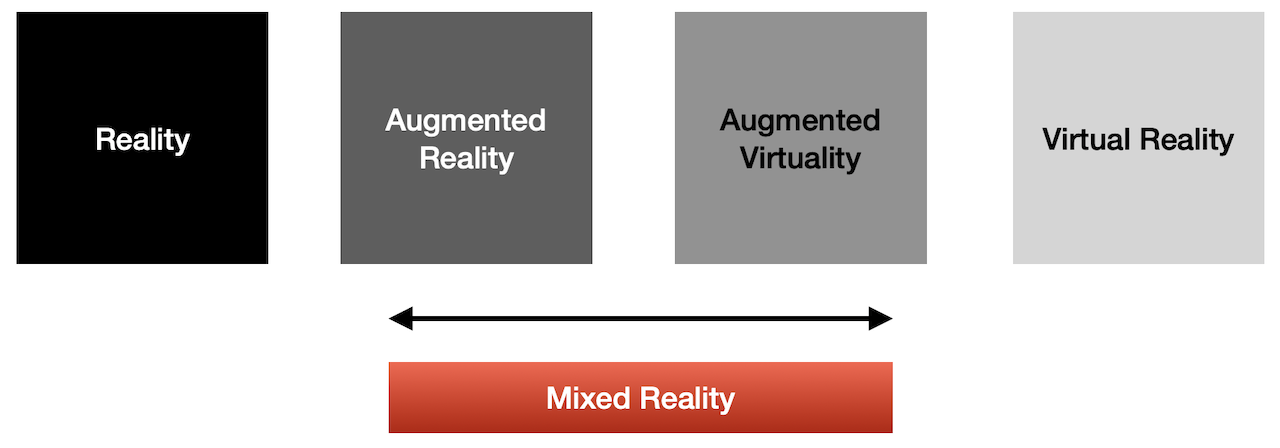
\includegraphics[width=0.7\textwidth]{img/continuum.png} 
%\captionsetup{justification=centering}
\caption{Milgram and Kishino Continuum}
% author: gabriel zalles ballivian (created using Apple Pages) [re-creation]
% public domain
\label{fig:continuum}
\end{figure}

Much like other authors in the field, if necessary, we will simply use the term AR in this text to avoid confusion. MR will be included in AR; we make no distinction between the two\footnote{It appears that MR is most prominent in industry products, however, fewer academic authors use this label.}. As new systems emerge, it is possible we will see even more types of "reality" emerge both in the academic and commercial sector. The lines are not always clear, especially when senses are stimulated by systems, or real-world stimuli, they were "intended" to be stimulated by. 

Consider a person seeing a VR experience with a VR display\footnote{Otherwise known as Head Mounted Displays (HMDs), these are "helmets" one wears which display images via screens mounted inside them. These will be covered in more detail in section \ref{subsec:hardware}.} but listening to sounds from speakers, which are inadvertently being blended with real world sounds. The confluence of synthetic and real stimuli in the auditory domain point towards an AR experience. However, what if the real world sounds are not intended to be there? Is one of their senses in AR, and another sense in VR? If the real world sounds subside, does that change how we label the experience? 

\section{History of XR}

Much, much before the first ever "real" VR experience was ever developed, pioneering painters, from as early as the 15th century, were already working on the concept of depth perception and optical perspective. Today we take for granted the idea that 2D representations of 3D space contain any dimensionality, but before the establishment of cameras, this was a feature which had to be creatively articulated by artists. The idea of a \textit{vanishing point}, the point at which receding parallel lines viewed in perspective appear to converge, shaped an entire generation of painters. Figure \ref{fig:san-pedro} shows Pietro Perugino's use of perspective in the "Entrega de las Llaves a San Pedro" fresco at the Sistine Chapel (1481–82).

\begin{figure}[!htb]
\minipage{0.5\textwidth}
  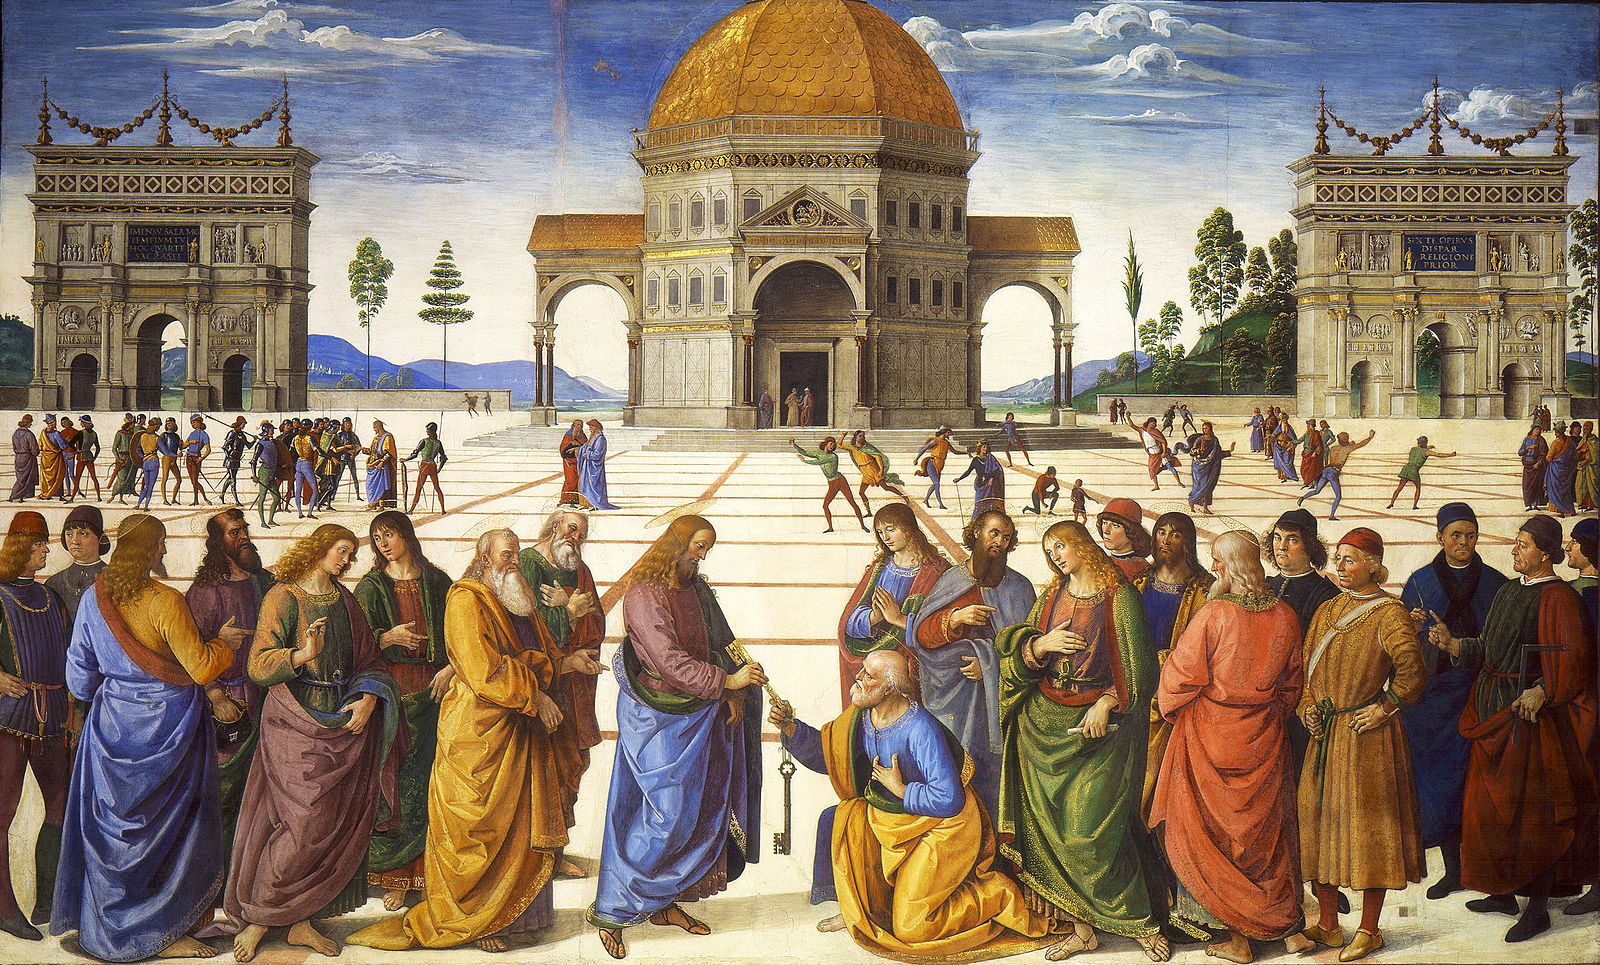
\includegraphics[width=\linewidth]{img/perugino.jpg}
  \caption{Vanishing Point Painting \cite{FileEntr24online}}\label{fig:san-pedro}
  % This work is in the public domain in its country of origin and other countries and areas where the copyright term is the author's life plus 100 years or fewer.
\endminipage\hfill
\minipage{0.5\textwidth}
  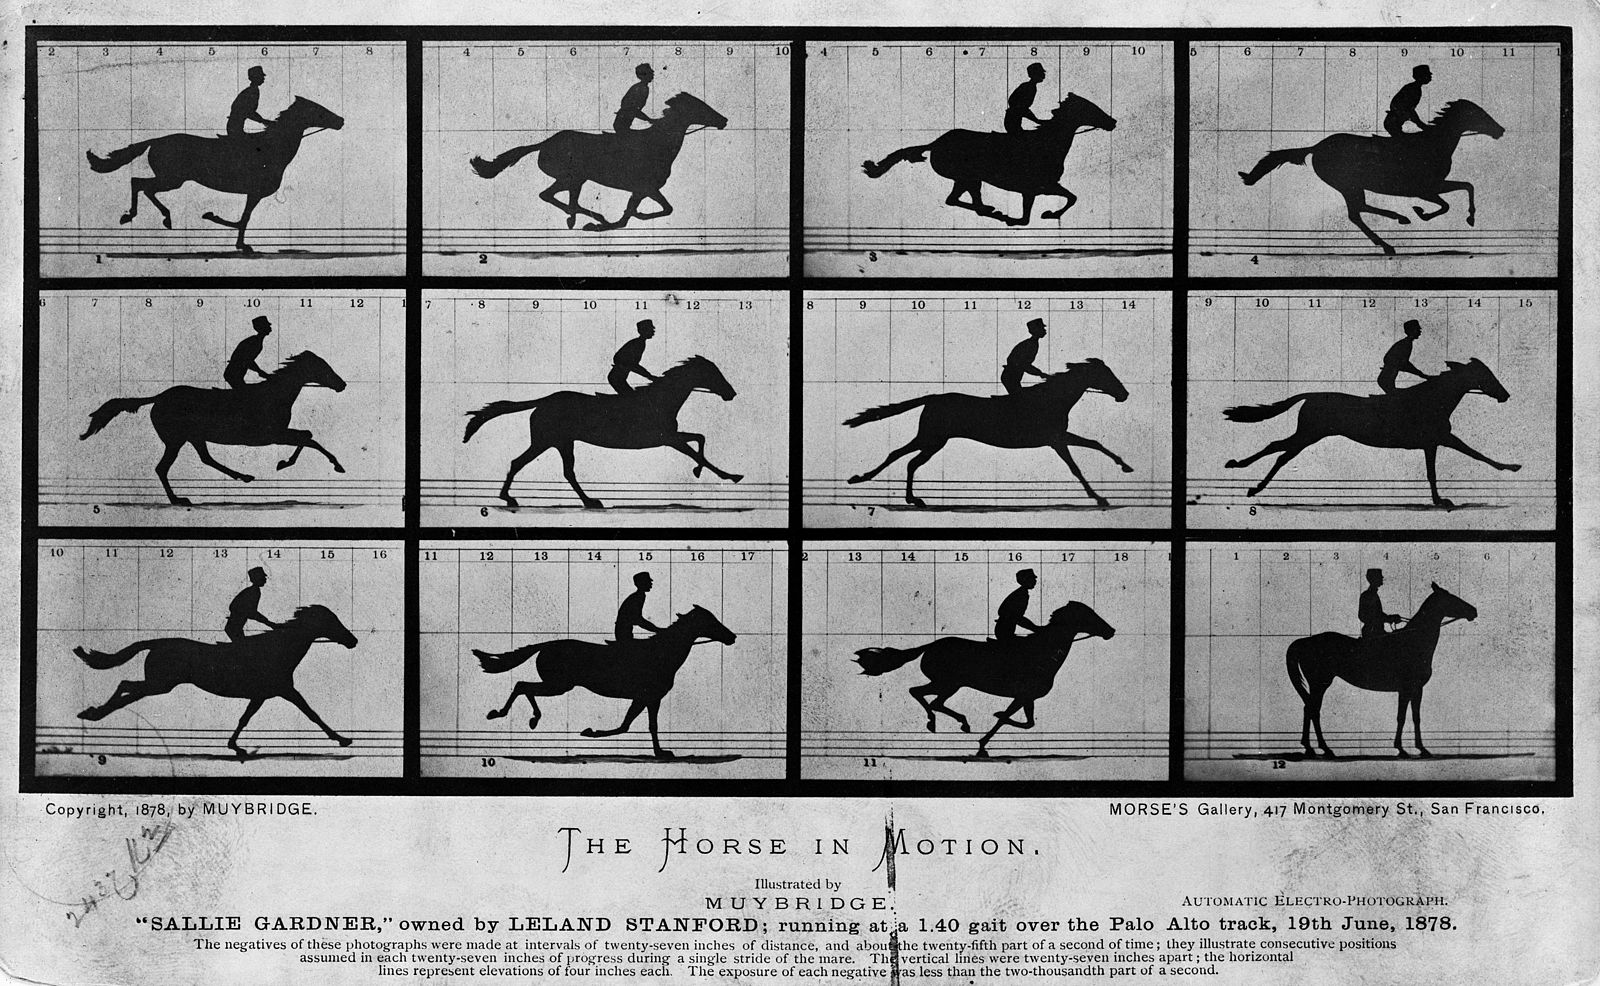
\includegraphics[width=\linewidth]{img/horse-in-mot.jpg}
  \caption{The Horse in Motion \cite{FileTheH64online}}\label{fig:horse-motion}
  % This work is in the public domain in the United States because it was published (or registered with the U.S. Copyright Office) before January 1, 1926.
\endminipage
\end{figure}

Much, much later, in the 19th century, the first \textit{stereoscope} was invented by Charles Wheatstone\footnote{English scientist and \href{https://en.wikipedia.org/wiki/Charles_Wheatstone}{inventor of many scientific breakthroughs.}} \cite{hemstrom2020comparison}. A stereoscope is a device in which a pair of slightly horizontally offset images of the same scene are presented to each eye, in order to provide additional depth perception. This exploits the fact that our visual system is always integrating two separate images, offset horizontally by the \textit{inter-ocular} distance, in normal viewing conditions. A picture of this device can be seen in Figure \ref{img:stereoscope}. In the 1930s, a portable version of a stereoscope called the \textit{ViewMaster} became commercially successful. The toy allowed people to switch images and see immersive photographs of places around the world. Some of the innovations of the stereoscope were the increased FoV and blocking of distracting boundary stimulus resulting in increased immersion. The ViewMaster, and other similar products, can seen as an early precursor to today's \textit{Head Mounted Displays} (HMDs), commonly used in VR experiences. 

\begin{figure}[ht!]%force figure here, top, strict
\centering
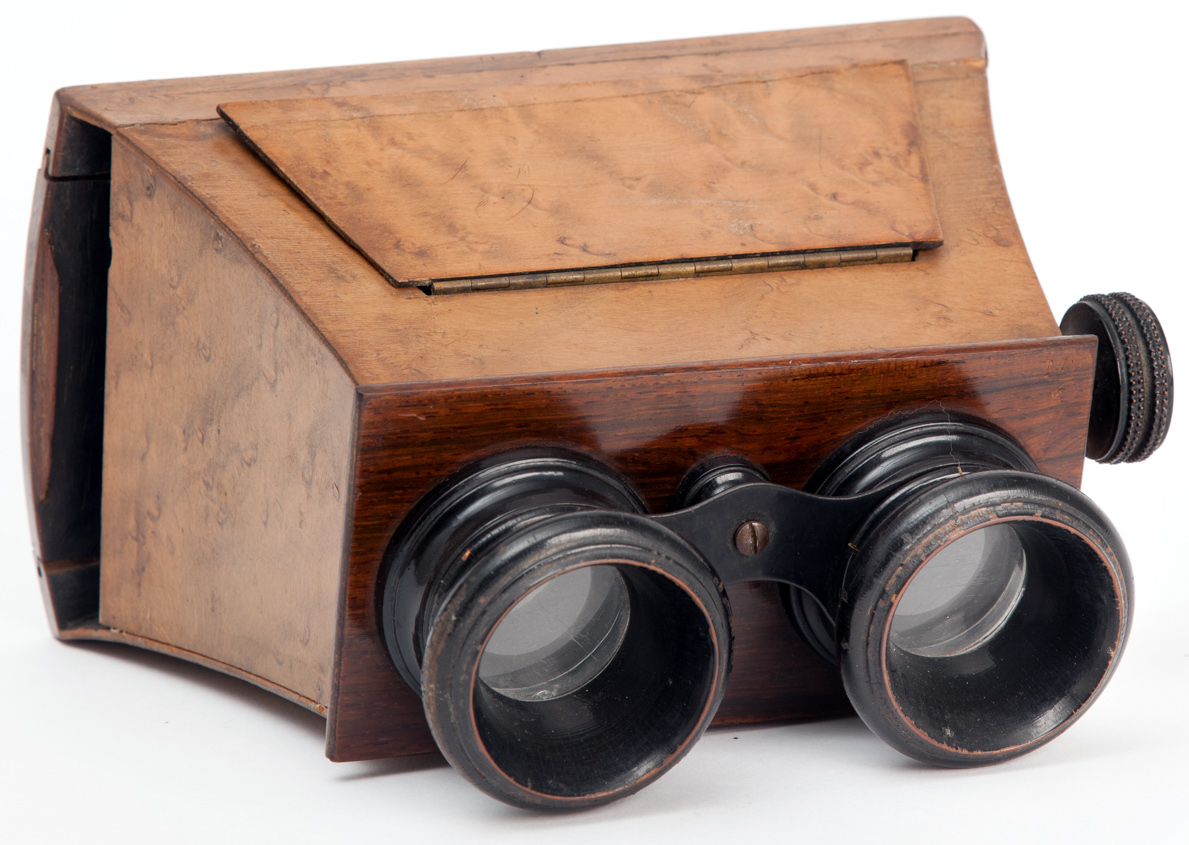
\includegraphics[width=0.4\textwidth]{img/stereoscope.jpg} 
%\captionsetup{justification=centering}
\caption{Brewster-type\protect\footnotemark stereoscope, 1870 \cite{FileIGB032online}}
\label{img:stereoscope}
\end{figure}

\footnotetext{Sir David Brewster (11 December 1781 – 10 February 1868) was a Scottish scientist, inventor, author, and academic administrator.}

In 1878, a few years after Wheatstone's stereoscope, one of the first examples of of \textit{stroboscopic apparent motion} was created by Eadweard Muybridge\footnote{Muybridge was an English photographer important for his pioneering work in studies of photographic motion (9 April 1830 – 8 May 1904)}. This effect refers to the ability to generate apparent motion by flipping through a sequence of images at a fast rate. Figure \ref{fig:horse-motion} shows Muybridge's famous work: "The Horse in Motion", which depicts several frames of a running horse, as it seemingly moves across space. In order to capture this sequence, 24 separate cameras were required. These were triggered by the horse as it moved along a track using ropes, which the horse's legs pulled on when running. The cameras were offset equidistantly to capture movements in a synchronized fashion. In order to reproduce the images, a \textit{zoopraxiscope}, also an invention of Muybridge's, was employed. The \href{https://upload.wikimedia.org/wikipedia/commons/0/06/The_zoopraxiscope-Horse_galloping-Animated.gif}{zoopraxiscope} is a disc containing multiple image frames which can be used to project a moving image in a recirculating fashion \cite{lavalle2016virtual}. 

Some 40 years later, in 1915, another well-known method in film-making used to increase realism was invented by Edwin S Porter\footnote{Edwin Stanton Porter (April 21, 1870 – April 30, 1941) was an American film pioneer, most famous as a producer, director, studio manager and cinematographer.}:\textit{3D film-making}. Modern 3D movies are created using special camera lenses and subsequently viewed using \textit{polarized} light filters. These filters, at the subjects eyes level, allow certain frequencies of light to pass into one eye, while blocking others. While there is a single image on the screen, two different images are perceived by each eye, much like with the stereoscope. \textit{Stereopsis} is the formal term describing the process of integrating two overlapping visual fields to achieve depth perception. 3D movies are still in use today in some VR experiences. They can also be found in commercial movie theatres across the world. 

\begin{figure}[ht!]%force figure here, top, strict
\centering
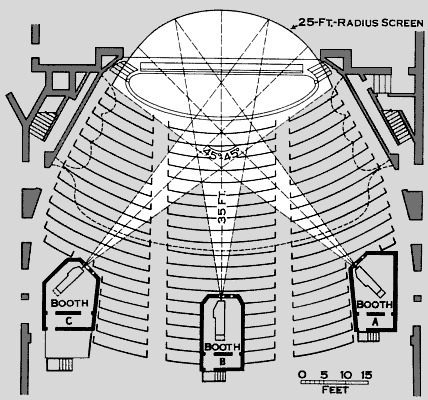
\includegraphics[width=0.5\textwidth]{img/cinerama.jpg} 
%\captionsetup{justification=centering}
\caption{Cinerama Diagram \cite{FileHowC90online}}
%public domain image
\label{img:cinerama}
\end{figure}

30 years later, a different technique was created to improve the sense of realism in movie systems. The method consisted of increasing the FoV by using a wider screen that surrounds the viewer, accounting for viewers' peripheral vision. The \textit{Cinerama}, from the 1950s, is an example of such a system. It used three projectors to extend the FoV and projected the image upon a concave surface for a richer viewing experience. It was created in the 1950s, and can be seen as a precursor to CAVE (Cave Automatic Virtual Environment) systems used for VR in the 90's\footnote{These are described in more detail later.}.

A few years later, in 1957, Morton Heilig introduced the \textit{Sensorama}, which combined: motion pictures, stereo sound, vibration, wind, and even smells, in a personalized stereoscopic \textit{multi-modal} experience. The device resembles an arcade machine with an enclosure surrounding the subject's head, in order to reduce distractions. Unfortunately, the Sensorama had a fixed perspective, which meant the user was limited to a single orientation. It was also very large and expensive, which ultimately led to its downfall. Figures \ref{img:cinerama} and \ref{img:sensorama} depict the Cinerama and Sensorama respectively.

\begin{figure}[ht!]%force figure here, top, strict
\centering
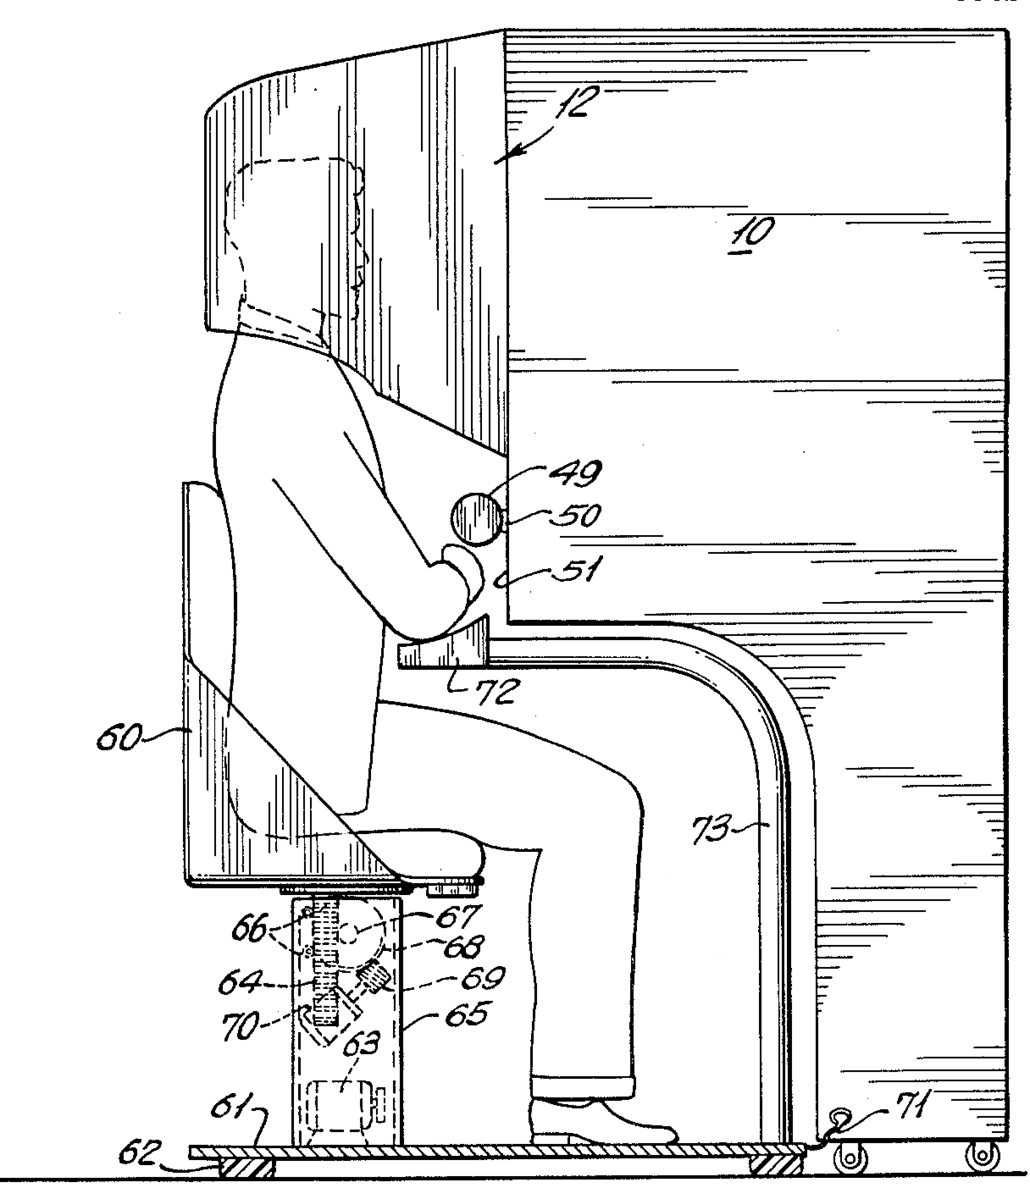
\includegraphics[width=0.4\textwidth]{img/sensorama.png} 
%\captionsetup{justification=centering}
\caption{Sensorama Patent Figure \cite{FileSens36online}}
%public domain image
\label{img:sensorama}
\end{figure}

Then, in 1965, a major step would be taken towards the realization of VR. That year, Ivan Sutherland\footnote{Ivan Sutherland (born May 16, 1938) is an American computer scientist and Internet pioneer, widely regarded as a pioneer of computer graphics.} introduced the concept of "The Ultimate Display", which he described as: "a room within which the computer can control the existence of matter." \cite{sutherland1965ultimate} A few years later, Sutherland and his team would build \textit{The Sword of Damocles}\footnote{You may find information regarding the myth \href{https://www.history.com/news/what-was-the-sword-of-damocles}{here}.}, regarded today as the first VR Head-Mounted Display (HMD). The display was a ceiling-suspended device capable of displaying simple wire-frame shapes according to the users' head movements \cite{hemstrom2020comparison}. This demonstrated for the first time in a virtual system the idea of the \textit{perception of stationarity}, which consists of making a static object appear to remain in its position while one moves their head. 

In the 1980s a number of advancements were made in the field, mainly by government agencies:

\begin{enumerate}
    \item In 1982, an advanced flight simulator called the \textit{Visually Coupled Airborne Systems Simulator} (VCASS) was created by the US Air-force Medical Research Laboratory.
    \item In 1984, the \textit{Virtual Visual Environment Display} (VIVED) was developed by the NASA Ames research center. 
    \item In the late 1980s, the term "Virtual Reality" was coined by Jaron Lanier, founder of the Visual Programming Lab (VPL). VPL would go on to develop the \textit{DataGlove} and the \textit{EyePhone} HMD. "Although all normal vision is lost wearing a HMD, the data glove allows the user to hold up their gloved hand in front of their face and see a digital representation through a HMD." \cite{dixon2006history}
\end{enumerate}

\begin{figure}[!htb]
\minipage{0.5\textwidth}
  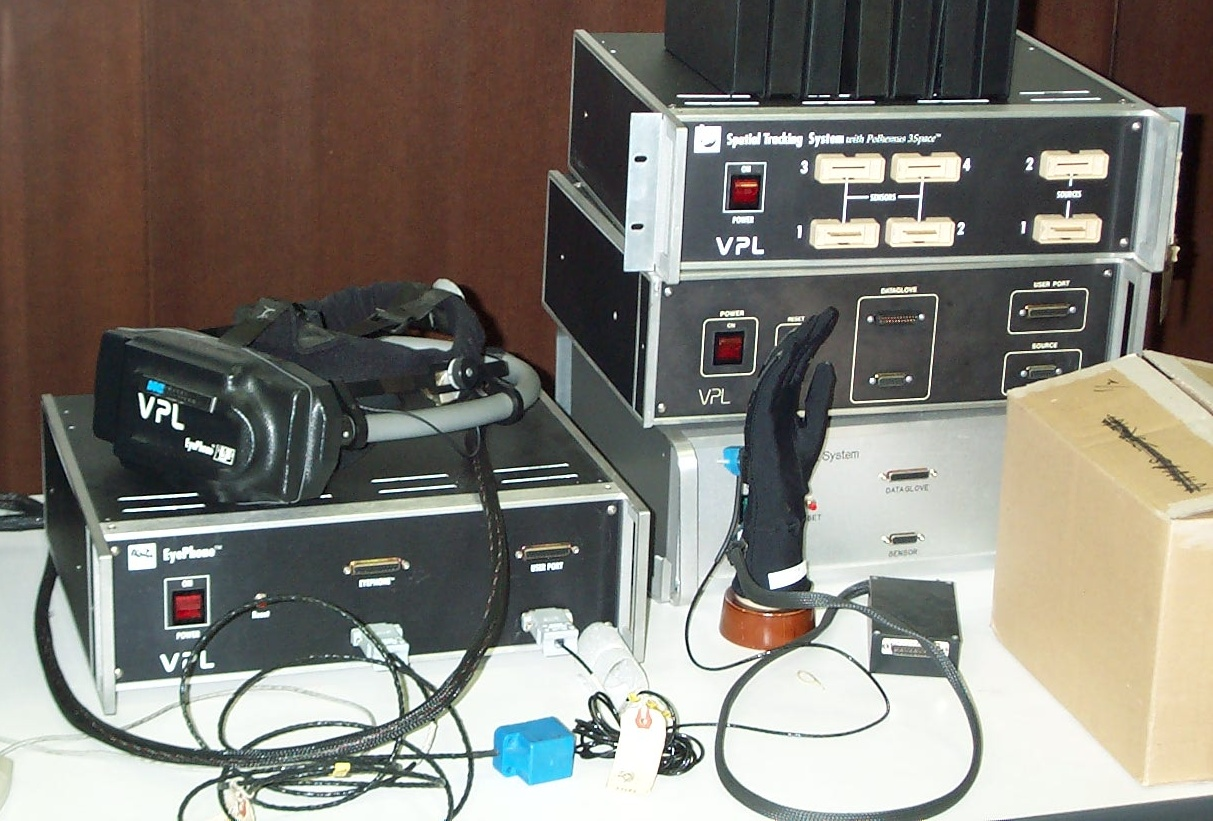
\includegraphics[width=\linewidth]{img/eyephone-dataglove.jpg}
  \caption{EyePhone HMD and DataGlove by VPL \cite{FileVPLE81online}}
  \label{fig:eyephone}
  %public domain
\endminipage\hfill
\minipage{0.5\textwidth}
  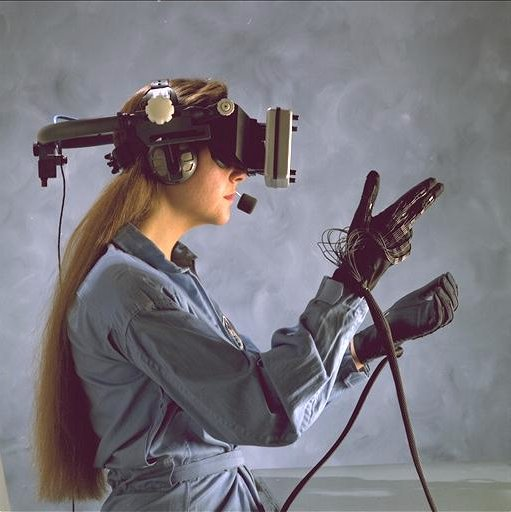
\includegraphics[width=\linewidth]{img/hmd-ames.jpg}
  \caption{HMD and Wired Gloves - Ames Research Center \cite{FileHead94online}}
  \label{fig:hmd-ames}
  %public domain
\endminipage
\end{figure}

Lanier went on to expand the DataGlove into a full body \textit{DataSuit}, capable of tracking users' different body joints. Using these suits, multiple users were able to interact inside a a virtual environment, and even change their physical appearance. In gaming, one's virtual representation is often called his or her \textit{avatar}.

A different approach, developed in the 90's, was the \textit{CAVE} (Cave Automatic Virtual Environment). This environment, developed in 1992 at the University of Illinois, uses a large number of projectors to, ideally, cover the entire surface of the room. Some CAVE systems also use 3D video in order to improve the depth perception of the image. The benefit of this approach is that the user does not need to wear any heavy equipment on their face which might restrict their ability to move. The downside is that such environments are often very costly to set-up given the large number of projectors needed to create the visual illusion. There are similar environments which use arrays of display panels in lieu of projectors to achieve higher visual fidelity.

\begin{figure}[ht!]%force figure here, top, strict
\centering
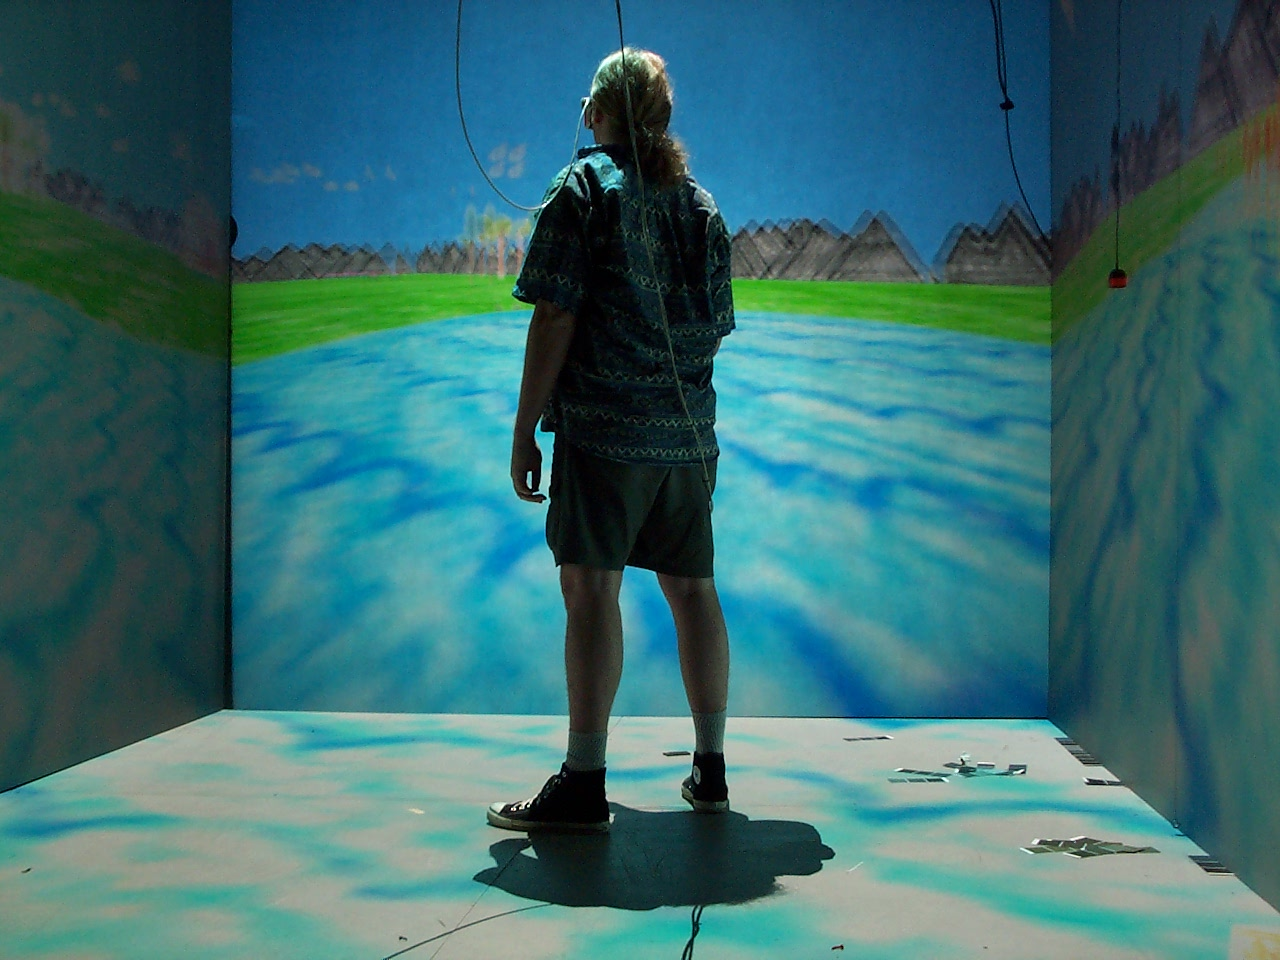
\includegraphics[width=0.6\textwidth]{img/cave.jpg} 
%\captionsetup{justification=centering}
\caption{CAVE \cite{FileCAVE71online}}
%public domain image
\label{img:cave}
\end{figure}

During this time there were also a small yet important number of artists who experimented with VR. Kazuhiko Hachiya created a two-person VR experience called \textit{Inter Discommunication Machine} in 1993, which switched one player's sight and sound for the others. The idea was to blur the lines between "you" and "me" \cite{dixon2006history} by switching sensory stimulation. At the Banff Centre, in Alberta, Canada, a number of VR projects were developed by a range of artists, all documented in Moser and McLeod's 1996 book "Immersed in Technology". Dixon \cite{dixon2006history} describes some of these projects in more detail. 

\section{Contemporary XR Techniques}

\subsection{Hardware} \label{subsec:hardware}

\subsubsection{Degrees of Freedom (DoF)}

Chapter 2 of LaValle's book \cite{lavalle2016virtual} provides us with an overview of hardware practices important to XR. An important distinction LaValle makes in regards to hardware, is control in either \textit{three degrees of freedom} (3DoF) or \textit{six degrees of freedom} (6DoF). An ordinary object moving and turning in 3D space has 6DoF. Three of its degrees of freedom correspond to its changing position in space. These \textit{translations} include: 

\begin{enumerate}
    \item Horizontal (side-to-side) or $y-axis$ motion.
    \item Vertical (up-down) or $z-axis$ motion.
    \item Distal (front-back) or $x-axis$ motion.
\end{enumerate}

The other three degrees of freedom include: roll, pitch and yaw, which correspond to rotations along the $x$, $y$ and $z$ axes\footnote{This is our preferred coordinate system, it should be noted that others exist.}. Sometimes the \textit{user} will be given only 3DoF, in which case this is normally in the form of rotation changes. This is generally the case when viewing 360\textdegree \ videos, for example: videos in which a scene is captured in every direction using spherical lenses or arrays of cameras. The person is able to experience all directions of the video, by moving their head, but, generally speaking, cannot change the point of capture. In other words, translations in space is restricted. In this case the \textit{tracking system} (ie. the sensors in the display) only provide 3DoF.

Some controllers, such as the Sony Playstation \textit{DualSense} controller, have only 3DoF, which means they can send rotational information but are not designed for translation tracking. Sony's VR ecosystem uses the \textit{Move Controller}, which has an LED that is tracked by a camera system, which, when paired with its internal sensors, allows 6DoF. Some HMDs offer 3DoF only, while others are paired with external sensors, which report the position of the HMD in space to the VR system. This is generally accomplished using external cameras which track lights on the HMD. Other, newer systems\footnote{For example the Oculus Quest.}, use internal cameras to perform this task. 

\begin{figure}[!htb]
\minipage{0.4\textwidth}
  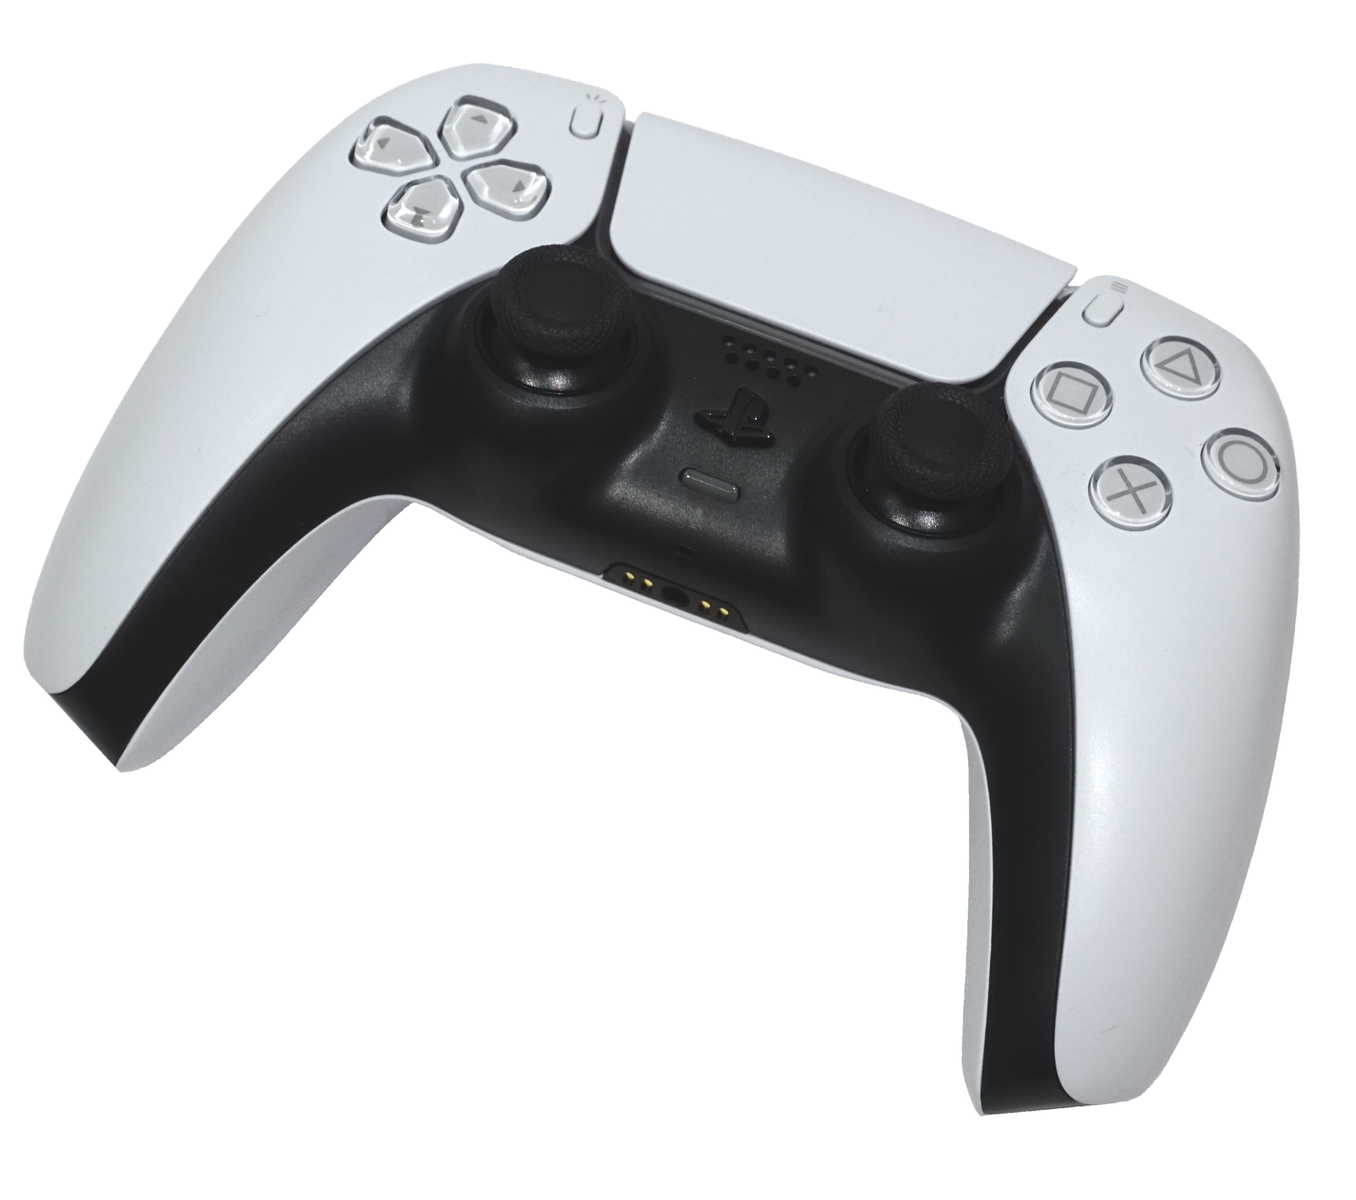
\includegraphics[width=\linewidth]{img/sony-dual.png}
  \caption{Sony DualSense Controller \cite{FilePlay5online}}\label{fig:sony-dual}
  % This file is licensed under the Creative Commons Attribution-Share Alike 4.0 International license.
\endminipage\hfill
\minipage{0.4\textwidth}
  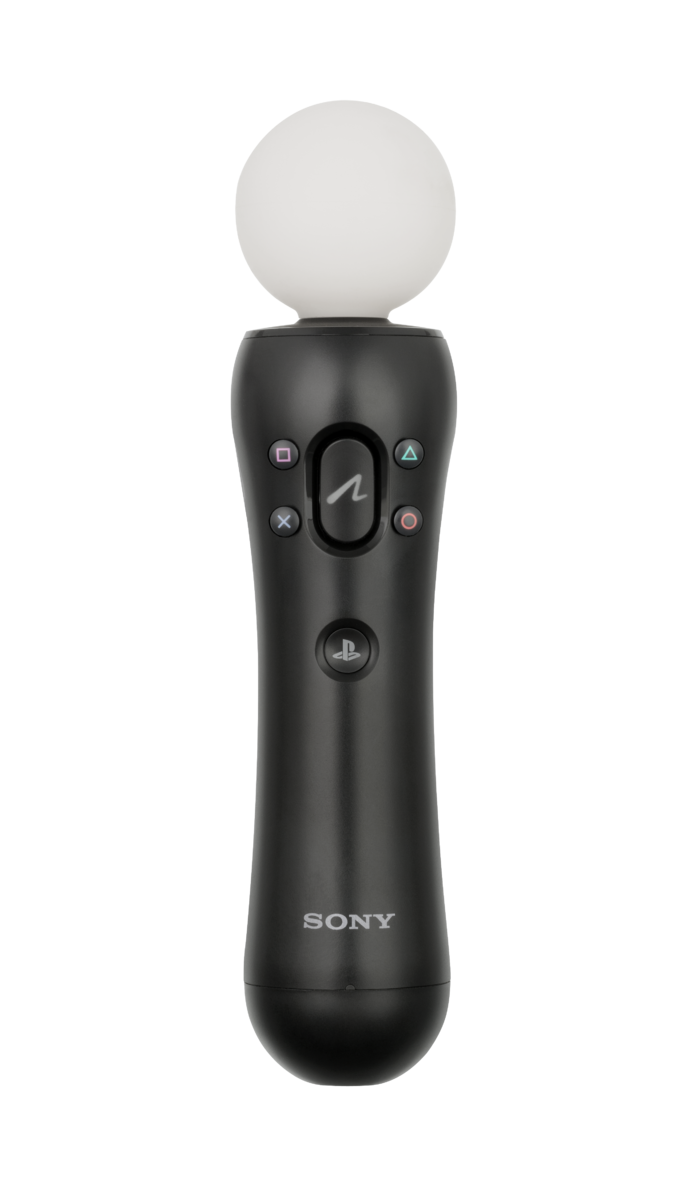
\includegraphics[width=\linewidth]{img/sony-move.png}
  \caption{Sony Move Controller \cite{FileSony89online}}\label{fig:sony-move}
  % public domain
\endminipage
\end{figure}

\subsubsection{World-fixed v. User-fixed}

Another important distinction we should make is between \textit{world-fixed} and \textit{user-fixed} systems. As we will see, user-fixed aural and visual displays offer a far more cost-effective and portable way of reproducing spatial audio and virtual scenes. World-fixed systems are less burdensome to the user, but often cost more to implement.

World-fixed systems refer to surround-sound systems, in the aural domain, and CAVE-like environments, in the visual domain. User-fixed systems refer contrastingly to binaural headphone systems and binocular HMDs, in the two respective domains. Both of these approaches to presenting XR experiences can be mixed. Each of them also have their own benefits and drawbacks. For sound systems, some of the key trade-offs between user and world fixed systems are:

\begin{enumerate}
    \item World-fixed systems require much more power (energy). Consider the power savings from binaural (headphone) reproduction versus surround-sound systems. 
    \item Headphones allow a sense of privacy, whereas surround-sound systems might disturb other people in your environment, or your neighbors. 
    \item User-fixed systems can be uncomfortable if used for long periods of time, since the user is required to wear heavy electronics on their head. 
    \item World-fixed systems might allow for multi-user experiences more seamlessly. However, there might be a noticeable drop-off in quality if users are outside the sweet-spot\footnote{Optimal viewing or listening position. HMDs and headphones do not have sweet spot problems.}. 
    \item Multi-user experiences are possible over headphones but require different sound processing for each user, which might prove computationally more expensive.
    \item Headphones are often much cheaper than surround-sound systems. 
\end{enumerate}

The trade-offs are quite similar in the visual domain. In world-fixed environments, it will only be necessary to modify the sound and visual scene according to users translational movements\footnote{If 6DoF is desired.}. Since they are already surrounded by audio-visual stimuli, natural rotational movements do not need to change anything in the environment. In contrast, user-fixed environments will need to adapt to user head rotations in order to create the illusion that they are inside an encompassing environment, which requires sophisticated graphics systems and a powerful computer.  

\subsubsection{VR Sickness}

An important problem to note here is poor updating of images in VR within user-fixed experiences. The slow frame-rate, or update speed, of these systems, can cause what is known as \textit{VR sickness}. This is caused by a mismatch in sensory information coming into the brain. This happens when one's \textit{vestibular} organs, used to maintain balance, are not in sync with one's visual organs. This is similar to the nauseating feeling we get when reading a book in a moving car. Over the years, GPUs\footnote{A Graphical Processing Units (GPU) is the part of the computer responsible for calculating and displaying images.} have become increasingly powerful, and, as a result, it is possible now to update images on HMDs quickly enough that VR sickness is eliminated\footnote{The amount of sensitivity to VR sickness is different from person to person, but, generally speaking, these systems work well enough now that they are mass produced and sold worldwide.}. CAVE-like environments do not suffer from this problem, however, much like in surround-sound systems, there is an optimal viewing area beyond which the image will not be of good enough quality. Ideally, in user-fixed systems, the frame rate is at least 90Hz, meaning there are 90 \textit{frames} per second. This number has become standard in the VR industry, since it seems to be the smallest frame-rate at which VR sickness is reduced to tolerable levels. 

\todo[inline]{Closed-loop vs. Open-loop}

\subsubsection{Dissecting XR Systems}

With the increasing pace of technological development, it can sometimes be difficult to categorize different systems and understand their relationship to the XR ecosystem. It is useful, in this context, to be able to dissect XR into its component part. Every XR systems can be divided into three primary parts \cite{lavalle2016virtual}:

\begin{enumerate}
    \item \textbf{Displays (output):} devices that stimulate your senses. %ch 4 and 5
    \item \textbf{Sensors (input):} devices that receive and interpret information from the real world. %ch 9
    \item \textbf{Computers:} devices which process inputs and outputs.
\end{enumerate}

% In the next few paragraphs we will describe these parts in more detail. 

\paragraph{Displays}

Displays, in the context of XR systems, refers to anything that is used to stimulate one's senses. They are simply outputs. Optical displays include projectors, such as in a CAVE, or HMDs - the counterpart to projectors in a user-fixed format. HMDs can be broken down into two main categories: \textit{dedicated HMDs}, and \textit{mobile HMDs}. Dedicated HMDs refer to visual displays whose function is solely to generate XR experiences. Dedicated HMDs can be broken down into two categories: \textit{tethered} and \textit{un-tethered}. 

As the name suggest, tethered HMDs require a direction connection to a computer, which sends video and power to the user's display. In turn, the tethered HMD also sends sensor information back to the computer, in order to update the displays in a cyclical fashion. Un-tethered HMDs refer to devices which have internal batteries, and powerful on-board processing units, allowing them to remain disconnected from an external computer. The GPU and CPU internally process any information needed, and wireless communication is possible with controllers and the web. 

Mobile HMDs, refer to HMDs which are based on mobile devices (ie. cellphones). Mobile HMDs are generally more cost-effective. However, since dedicated un-tethered HMDs are designed solely for the purpose of generating XR content, their internal components make them better at this task than most mobile-based systems. They are also substantially larger than mobile phones, which means they can hold bigger batteries and more computing power. On the software side, mobile HMDs operate either via standalone apps or WebXR solutions, both of which we will discuss in more detail later. 

\begin{figure}[ht!]%force figure here, top, strict
\centering
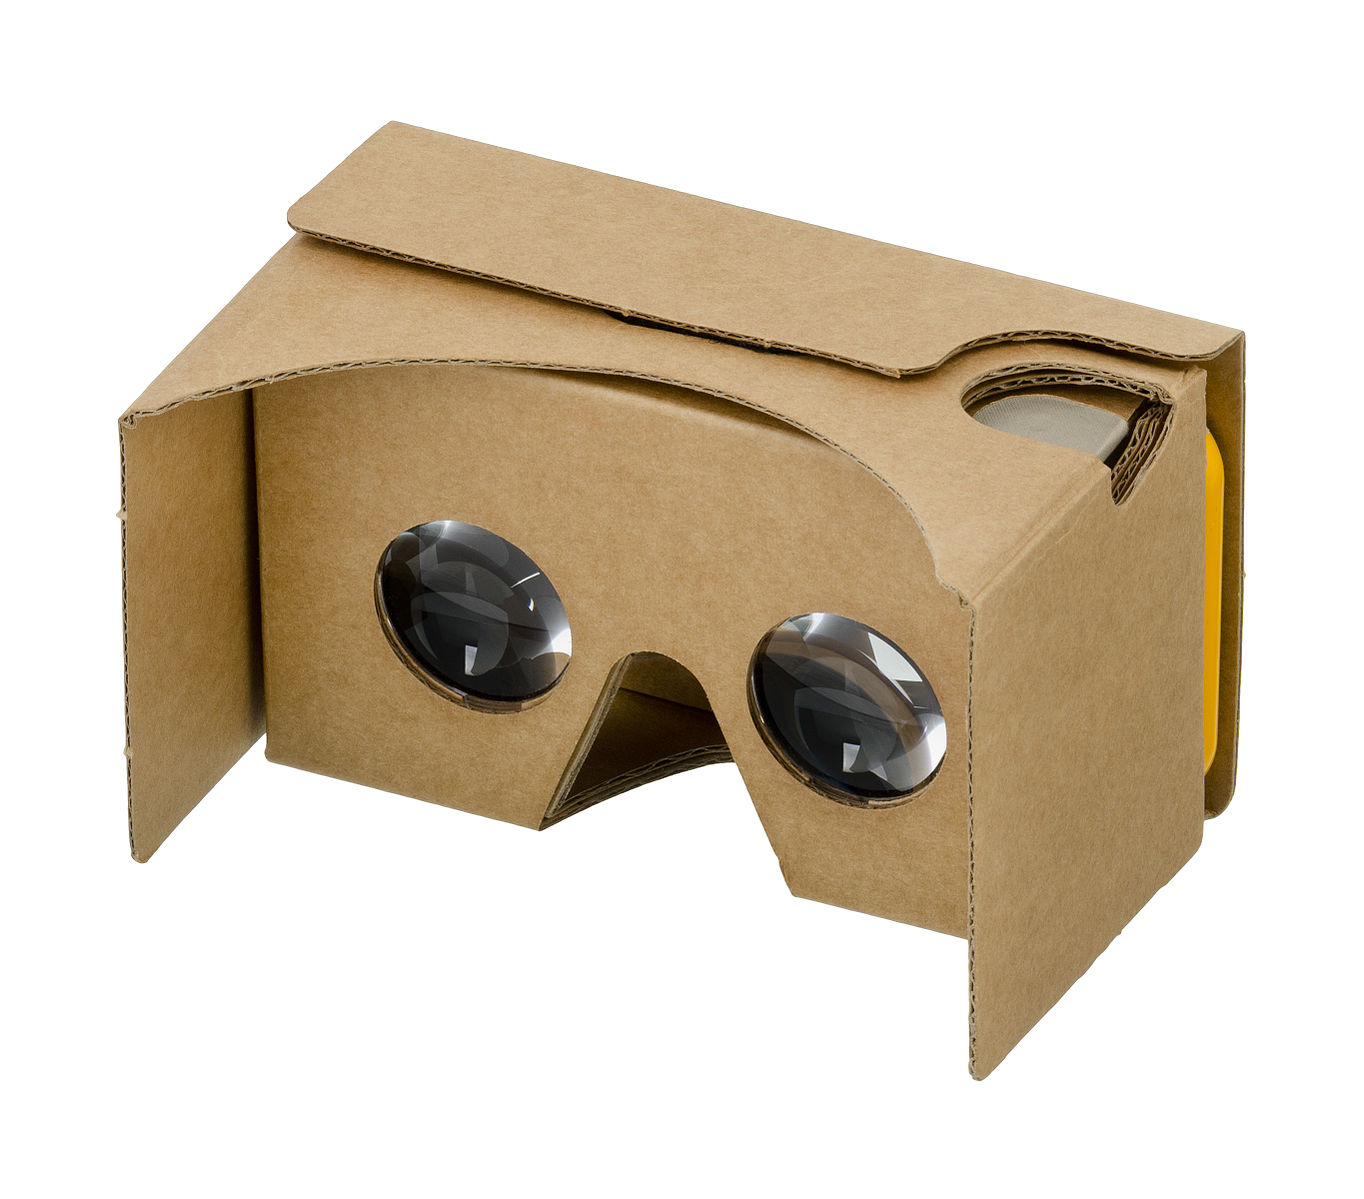
\includegraphics[width=0.5\textwidth]{img/cardboard.jpg} 
%\captionsetup{justification=centering}
\caption{Google Cardboard \cite{FileGoog63online}}
%public domain
\label{img:cardboard}
\end{figure}

An example of a mobile HMD is Google's \textit{Cardboard}, seen in Figure \ref{img:cardboard}. This simple HMD made out of cardboard can be used together with a smartphone to experience VR content with acceptable quality. It became popular in 2015, when the New York Times distributed the unfolded device to subscribers along with an app for VR journalism, focusing on the Syrian refugee crisis\footnote{The name of the aforementioned video is: "Displaced", by authors Ben C. Solomon and Imraan Ismail \cite{TheDispl63online}.}. Much like with other HMDs, two small magnifying lenses, usually \textit{Fresnel lenses}, are situated in front of the eyes. 

XR displays can also be found in the aural domain. These include surround-sound systems, headphones, or \textit{bone-conduction headphones}. Bone-conduction headphones send vibrations directly to the skull which is connected to our auditory system. There are also some XR HMDs which use small speakers near the ears to provide an auditory AR experience. Additionally, there are displays for our other senses. The most commonly encountered display for \textit{haptic} feedback is vibration systems, which are used in controllers. 

AR HMDs offer another form of optical display. Rather than placing screens in front of the subjects eyes, these place transparent surfaces upon which light is emitted. This allows the user to see both the real world and additional objects the experience provides. Figure \ref{img:ar-glasses} shows a man wearing a pair of AR Glasses. 

\begin{figure}[ht!]%force figure here, top, strict
\centering
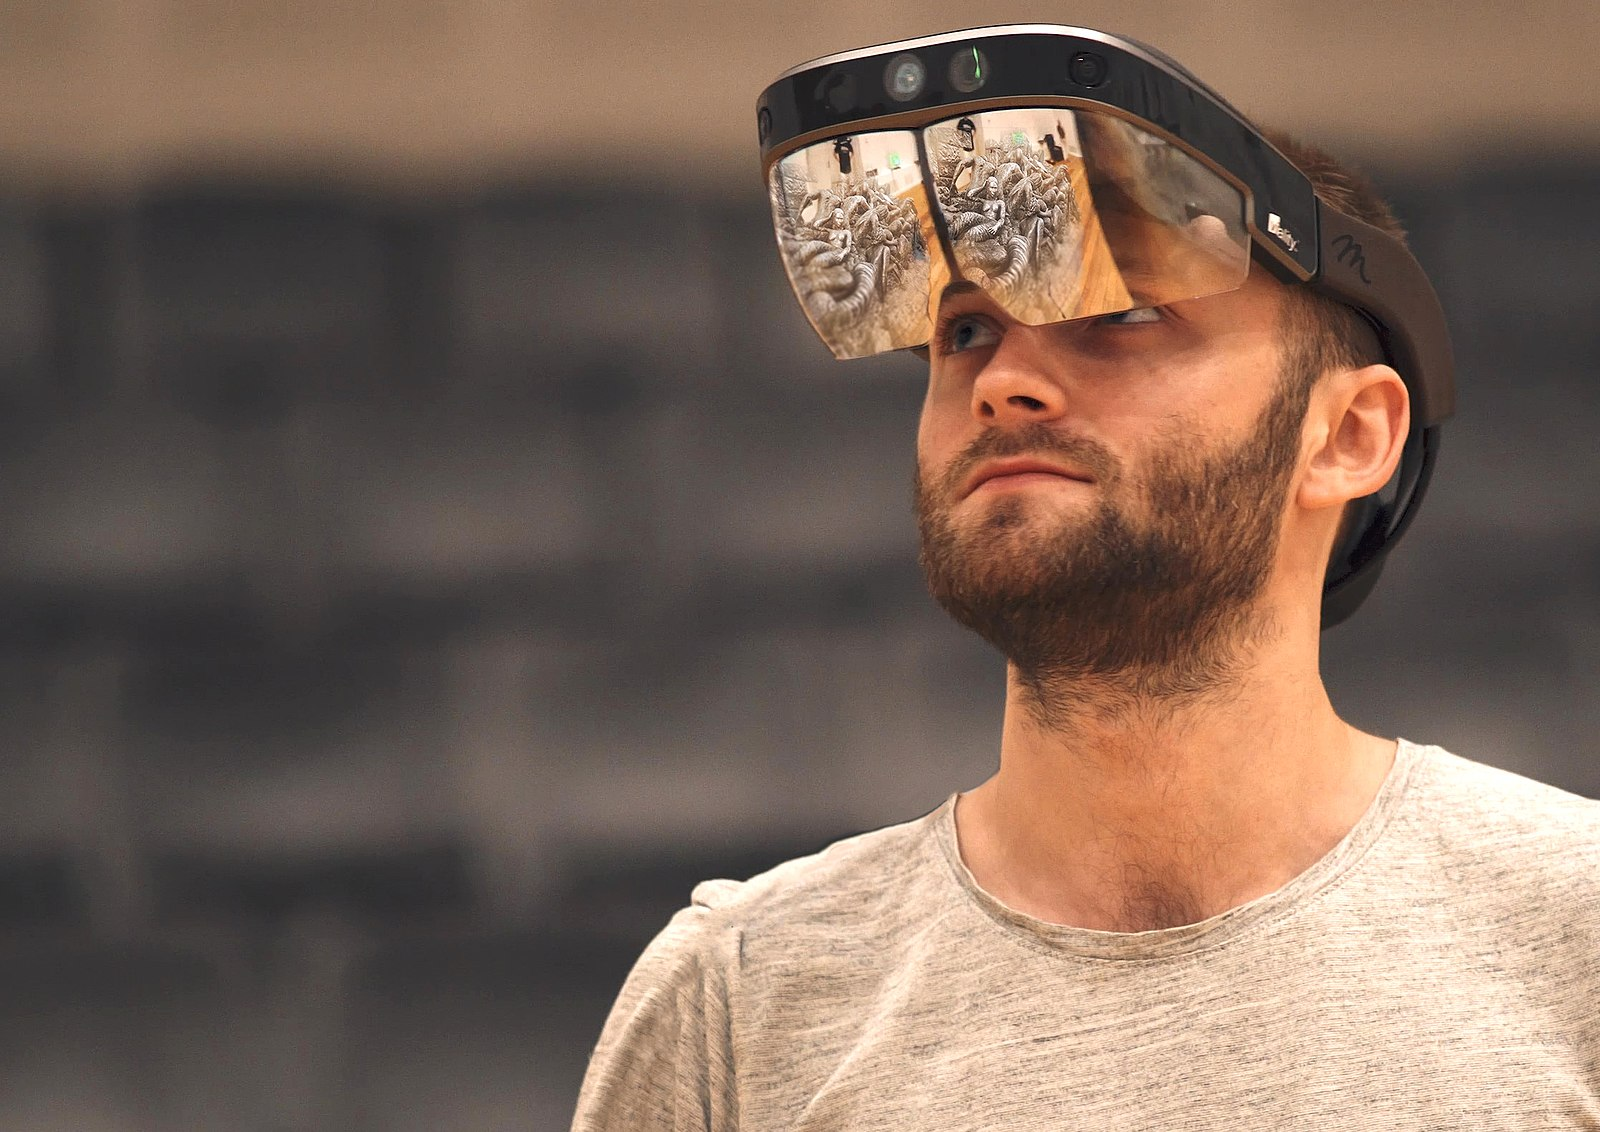
\includegraphics[width=0.6\textwidth]{img/ar-glasses.jpg} 
%\captionsetup{justification=centering}
\caption{Man Wearing AR Glasses \cite{FileWear23online}}
%Creative Commons Attribution-Share Alike 4.0 International license.
\label{img:ar-glasses}
\end{figure}

\paragraph{Sensors}

Sensors refer to inputs the computer-system will receive in order to accurately render the scene for the user. The most salient information needed for XR applications employing HMDs is gyroscopic data. Gyroscope are embedded in most of today's cellphones, and all dedicated HMDs. These report the orientation of the user's head back to the rendering software. Gyroscopes are also sometimes found inside controllers, such as inside the Sony Move Controller we showed earlier. 

The number of controllers, or sensing systems, available today is exceedingly large. It would be impossible to list them all here. Instead we provide a short list of some additional popular sensors: 

\begin{enumerate}
    \item \textbf{The Leap Motion Controller}: is an infrared camera system used to detect and track human hands, including independent joint movements and fingers. It can be used in lieu of VR controllers.
    
    \item \textbf{Microsoft Kinect}: is a camera and \textit{infrared} sensor system capable to performing depth mapping, and track entire bodies. It can be used to track body orientation and movement of large appendages. This is accomplished by projecting infrared light unto surfaces and capturing the reflection. 
    
    \item \textbf{Game Controllers:} many people familiar with game controllers, such as those from Sony or Microsoft, prefer playing in VR using these standard controllers - over \textit{VR controllers} - even though some only provide 3DoF. An example of a game controller is the Sony DualSense Controller.
    
    \item \textbf{MOCAP}: a MOtion CAPture systems, is similar to a Kinect, but capable of tracking bodies in a larger area, and uses multiple camera angles. This means that subjects do not need to face any particular direction. In order to track limbs, special suits which reflective balls are worn by subjects. These are specialized systems, and tend to be more costly than mass produced video game devices. 
    \item \textbf{VR Controllers}: in addition to the Sony Move Controller there are various designs by Oculus\footnote{A Facebook subsidiary.} and \href{https://www.htc.com/us/}{HTC}. Some other HMDs, especially those for MR, use cameras to track fingers, much like a leap motion would. 
    
    \item \textbf{Facial Tracking}: this type of input is more common in AR applications. The technology allows detection of faces and analyzes facial expressions. Digital masks or filters can follow the movements of the face. 
\end{enumerate}

In addition to all these devices some people also opt to use a standard keyboard and mouse system for interacting in XR. There are also custom-made sensing devices out there created from prototyping parts which can communicate to the software via wireless protocols. Finally, there are various specialized controllers designed for specific tasks, such as controllers resembling plastic rifles, used in war games, for example.

\begin{figure}[ht!]%force figure here, top, strict
\centering
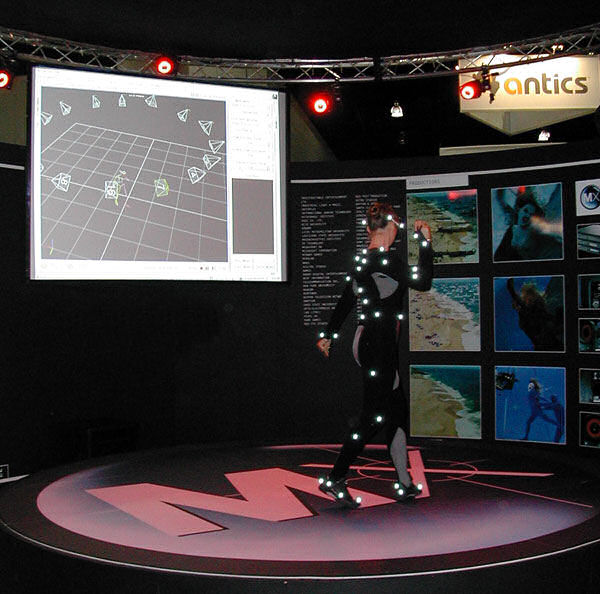
\includegraphics[width=0.75\textwidth]{img/mocap.jpg} 
%\captionsetup{justification=centering}
\caption{MOCAP System \cite{FileMoti99online}}
%public domain
\label{img:mocap}
\end{figure}

One of the complications that can sometimes arise in sensor or controller design is the problem of \textit{registration} in VR. If the objects are not registered, because they are not tracked by the system, then the person has no way of locating the object in the real world. Some companies provide locators which allow users to register different objects in VR by attaching any 3D model they want to the object. For example, one can specify a real guitar is being used and attach the model of a guitar to the hands of the user - allowing them to find their guitar once inside VR. This is one of the advantages of AR over VR: there is only partial \textit{occlusion}; as a result, subjects can easily locate the items they wish to interact with in the real world.

Certain successful designs exploit \textit{proprioception}, which is our sense of where our extremities are without having to see them. For example, with the aforementioned Kinect, we don't necessarily need to see a representation of our body in VR to know where our appendages are. We can easily perform any movements the system requires without directly needing to see them happen. In most cases, however, registration of sensors is preferable, as they give users direct feedback to confirm the actions they are undertaking. 

\paragraph{Computers}

Once all the inputs and outputs are known, it is the task of the computer to analyze incoming data and present stimuli to the user via various displays. The capabilities of the computer will determine how much data it can analyze and how much data it can return. As we have noted, some cellphones are able to generate virtual worlds, however, because these have less powerful computing hardware, the graphic scenes generally need to be simpler. 

Within the computing hardware, there are various sub-systems which work together to provide a smooth experience. The \textit{Graphical Processing Unit} (GPU), is responsible to \textit{rendering}\footnote{Calculating vertex, edge, and face positions, and subsequently displaying them. They also perform lighting and shadowing.} the graphical content. The \textit{Central Processing Unit} (CPU) is similar to the GPU, however, is not designed for graphics - instead it handles all the other calculations, commands and processes necessary. In some designs, a \textit{Micro-Controller Unit} (MCU) is also used to handle inputs and relay the information to the CPU, which may be tethered to or inside the HMD.

Some of the important factors to consider here are portability and also the ease of prototyping. When developers are creating these experiences, they need a way to quickly create environments and test them out. Wireless devices might prove more difficult to work with in this regard.

\todo[inline]{display interface chips?}

\section{Software}

Generally speaking, today, there are three main platforms that are \textit{targeted} by game developers. For each of these different targets, there are associated software libraries that allow us to create content. \textit{Game engines} are the most powerful of these three platforms. These software environments are designed to facilitate the creation and customization of video games and XR experiences. Secondly, there are mobile apps, for which there exist various different \textit{Software Development Kits} (SDKs) with different flavors depending on the \textit{operating system} (OS) of the mobile device. Finally, there is \textit{WebXR}. This corresponds to applications that run on the browser, be it via a mobile phone, HMD, or a traditional desktop computer. 

\subsection{Game Engines}
% Unity, Unreal, Godot, etc.

Game engines are software-development environments used to create video games or XR experiences. The core functionalities of these engines include:

\begin{enumerate}
    \item \textbf{3D graphics}: determines how objects are displayed on screen. It should, for example, consider vanishing point, occlusion and parallax. 
    \item \textbf{Physics engine}: determines how light scatters, objects move, and other attempts to simulate real world physical behaviors. 
    \item \textbf{Collision detection}: responsible for detecting contact between objects. 
    \item \textbf{Sound}: this might include spatial audio systems, which simulate 360\textdegree \ sound using \textit{binaural} filters.
    \item \textbf{Scripting}: the ability to customize behaviors based on developer needs. 
    \item \textbf{Animation}: importing objects with built in movement behaviors. For example, a model of a bird with its wings flapping.
\end{enumerate}

Today, the most popular game engine is likely \href{https://unity.com/}{Unity} which is cross-platform\footnote{Works with multiple operating systems, including Linux.} and allows \textit{building}, or targeting, a multitude of platforms, including: Mac, Windows, WebGL, iOS, and WebGL - to name a few. Unfortunately, the license is proprietary - however it does offer exclusive support for educational purposes, making it a useful tool for pedagogical purposes. Another game engine that is gaining popularity, due to its open source nature, is \href{https://godotengine.org/}{Godot}. This game engine, however, is not as well-featured as Unity, given that it is much younger. One final game engine we should mention is \href{https://www.unrealengine.com/en-US/}{Unreal} which is commercial in nature but whose \textit{source code} is available online. 

All of these game engines, as far as XR is concerned, are suited for creating content targeting HMDs, however world-fixed systems do not seem to be natively supported. Tredinnick et al. \cite{unicave2017} propose a plug-in for the game engine Unity, which allows one to use the software with "distributed immersive tiled or projection-based VR display systems", such as a CAVE. It is possible to use internal audio routing software to decode ambisonics from other software, but perhaps one could also develop a plug-in which allowed for this natively. 

\subsection{Mobile XR}

Mobile XR SDKs are used to develop apps and experiences which can be downloaded and run on cellphones. Sometimes these experiences come in the form of 360\textdegree \ videos, other times the applications are graphical renderings of scenes composed in game engines. Various large technology companies, such as Google and Samsung, have created Mobile XR development libraries. In the next few sections, we will explore some of these projects. It should be noted that, with the proliferation of standalone HMDs, mobile VR SDKs are beginning to lose support from these companies. We believe it is only a matter of time before most of these development platforms are entirely irrelevant in the VR ecosystem. Mobile AR SDKs are still being supported, and are finding new applications every day.

\subsubsection{Mobile VR}

Mobile VR SDKs are development kits used to create VR applications targeting mobile devices. The three most popular platform in this area are the: Google \textit{Cardboard}, Google \textit{Daydream}, and Samsung's \textit{Gear VR}. Each of these different platforms has different SDKs which allows users to create VR experiences for them. Some of these different platforms are proprietary, and, as a result, there are limits to what developers can do with them. 

Unfortunately for consumers, over the last few years mobile VR SDKs have lost a lot of support\footnote{Time of writing 2021.}. This is due to the fact that both Google and Oculus\footnote{Gear VR was a collaboration between Samsung and Oculus.} have transitioned into selling standalone HMDs. Fortunately, Google still supports the Cardboard environment to create VR experiences. Since the Daydream project and Gear VR project are now both considered \textit{legacy}\footnote{Outdated systems, in computer science parlance.} systems, we will discuss a bit here only about the Cardboard environment. 

\paragraph{Cardboard SDK}

The recent releases of the Cardboard SDK by Google allow developers to target iOS and Android devices. One can also use the SDK inside Unity if desired. The SDK is licensed under \href{https://www.apache.org/licenses/LICENSE-2.0.html}{Apache License 2.0}. Given the simple nature of the Cardboard HMD, the \textit{Application Programming Interface} (API) only allows for monitoring the input of a single button. Naturally, the system also performs motion tracking and stereoscopic rendering, both requirements for VR. Because of the interactive limitations of the system, most of the apps for this system are simple content-viewing apps. One example of these is the \textit{Within VR} app which features political, kids, and scientific 360\textdegree \ videos. 

\subsubsection{Mobile AR}

Mobile XR comes in two types: \textit{native} and web-based applications. For example, within mobile VR, viewing a Youtube video that is \textit{streaming} from the browser can be considered a web-based application. Meanwhile, with apps like \textit{Within VR}, the user downloads these videos in their entirety before viewing. This is a native application that does not rely on a browser or an internet connection after the video has been downloaded. 

Mobile AR also comes in these two styles; Web-based applications will be discussed in more detail later, in this section we will only discuss software platforms used to develop native mobile AR applications. iOS and Android are the two most common OSs for mobile devices today, and both offer different SDKs to create AR applications. In the next few paragraphs we will discuss some of the features of the most popular SDKs for mobile AR applications. 

\paragraph{ARCore}

ARCore is an \href{https://github.com/google-ar}{open-source Google project}\footnote{Apache License Version 2.0.} allowing one to create AR apps for Android or iOS. It can also integrate with Unity or Unreal. Its main features include \textit{motion tracking}, \textit{environmental understanding}, and, \textit{light estimation} \cite{Fundamen38online}. One can also use the SDK for developing WebXR applications. There is an Android \textit{Native Development Kit} (NDK) written in C, and an SDK written in Java which gives programmers flexibility. The following list describes in some more detail the features of this development library.

\begin{enumerate}
    \item \textbf{Motion tracking}: ARCore uses \textit{Simultaneous Localization And Mapping} (SLAM) to "understand where the phone is relative to the world around it" \cite{Fundamen38online}. The camera detects \textit{feature points} and combines the information with IMU data to estimate the position and orientation\footnote{In the API the combination of position and orientation is called \textit{pose}.}
    \item \textbf{Environmental understanding}: the library is also able to detect certain features such as planes from the cluster of data. It uses this information to place objects on flat surfaces. 
    \item \textbf{Depth understanding}: the system can create depth maps using RGB\footnote{Red, Green, Blue.} data from the main camera. 
    \item \textbf{Light estimation}: ARCore also detects and understand shadows, and attempts to shade virtual objects using natural shadows. This is done to improve the sense of realism. 
\end{enumerate}

\todo[inline]{More info on SLAM? Importing point-clouds to Unity?}

In addition to this, the system allows for\textit{ user interaction}, \textit{oriented points}, \textit{anchors} and \textit{trackables}. In order to provide interactions \textit{hit testing} methods are provided. This casts a ray using the \textit{pose} of the mobile device and reports what objects, if any, have collided with the ray. The oriented points feature is used to place objects on angled surfaces. Anchors are positions where virtual objects are anchored, as the name suggests, while trackables are real world objects the system tracks over time. Finally, the library is also capable of \textit{augmenting 2D images}\footnote{Adding virtual objects to specific 2D images.} and contains methods for \textit{cloud anchoring} which allows multiple "users have the same AR experience simultaneously" \cite{Fundamen38online}.  

\todo[inline]{Music projects that used it?}

\paragraph{ARKit}

While not open-source, this SDK by Apple provides some insight into state-of-the-art systems that are already widely available and might inform the next generation of spatial instruments and systems. Many of the functionalities of ARCore can be found in ARKit. One of the big developments, in the new line of iOS devices, is the introduction of a \textit{LiDAR} scanner, which allows for more accurate spatial mapping. LiDAR, or "Light Detection And Ranging", is a method for determining distances by pointing lasers at one or more points, and measuring the time it takes for the reflected ray to return. According to Choi \cite{choi2017range}, the Kinect sensor mentioned earlier is a \textit{structured light} sensor, making subtly different than LiDAR\footnote{In fact, Kinect versions I and II use different mechanisms for 3D scanning. Kinect II uses a \textit{Time of Flight} (TOF) mechanism.}. Choi describes the principle behind LiDAR:

\begin{quote}
    "LiDAR systems use a single laser beam, which enables the sensing to measure the distances of far objects up to few kilometers because of the focused laser beam. To provide multiple 3D points of a scene, the laser beam can be scanned by a rotating mirror."
\end{quote}

Much like ARCore, anchors can be placed inside the scene to fix virtual objects. These anchors can be integrated with maps so objects can be placed around the world. The library also has facial tracking support for multiple people simultaneously and the ability to deploy collaborative sessions. One of the big limitations Apple however is the high cost of these devices and the proprietary nature of the code, which does not allow as much freedom to developers. Also, unlike ARCore, ARKit can only target iOS devices. 

\subsection{The OS}

Before we move on to WebXR, which is OS-agnostic\footnote{This is only true in desktop OSs, mobile device OSs still create barriers. The best OS for WebXR on mobile devices is Android at the moment.}, we should talk about how different desktop computer OSs affect the ability to create and deploy XR experiences. Many people who own and operate OSx know that the development of XR applications is currently limited in this OS. Most of the state-of-the-art GPUs and software needed to play, or develop, XR experiences, unfortunately do not work well with OSx. 

Windows is the preferred OS for people working with XR, and is the most supported out of the big three - Linux and its various flavors being the third major OS. The major reason for this seems to be the cost of the hardware and lack of customization for Apple devices. Apple has focused more of its attention on AR experiences for mobile devices and tablets. Linux at this point has very little support for XR experiences\footnote{Time of writing April, 2021.}. The main problems with Linux are the drivers for the GPUs and proprietary software for XR which cannot be fixed by FOSS developers. 

This perhaps is another great argument for prioritizing development in WebXR, rather than OS-specific software. The main bottleneck with WebXR is the way programs are loaded. Instead of downloading executable files, WebXR requires temporary downloads which live in \textit{Random Access Memory} (RAM). This means that devices with less RAM will have trouble running these experiences smoothly. 

\todo[inline]{Middleware like FMOD and Wwise? What is SteamVR, is it also middleware?}

\subsection{WebXR}

WebXR refers to VR or AR applications that run on the browser. In contrast to mobile or computer applications that load assets and code from a hard disk, after the application has been downloaded, these applications dynamically, and temporarily, access data from one or more servers. One clear limitation of these systems, as a result, is that a constant, good quality, network connection, is required for the experience to perform smoothly. These program also reside in RAM, as pointed out earlier, which means they must be relatively small. 

WebXR has some clear benefits when compared to native XR applications that run on mobile devices or personal computers. One of the main benefits of these systems is their flexibility and interoperability across devices. In contrast to other systems, WebXR applications tend to work on most devices connected to the internet, so long as a modern browser, which supports WebXR, is used\footnote{WebXR in iOS has very limited support. Luckily, Apple users can still see experiences on desktop Browsers. Mozilla created a \href{https://webxr-ios.webxrexperiments.com/}{WebXR Viewer} for iOS.}. A list of OSs that work with WebXR can be found \href{https://webvr.rocks/}{here}\footnote{Site accessed April, 2021.}. 

In contrast, when one develops and builds an application for one particular OS, it is not always the case that the same application can be built seamlessly for another OS. Another virtue of WebXR is that a HMD is not required to attain a partial degree of immersion. There are various XR experiences built on the web for HMDs, which can be experienced over a computer or cellphone. While not fully immersive, this allows people who feel uncomfortable with wearing HMDs to experience an artist's work, at least to a limited degree. 

\subsubsection{WebAR}
\paragraph{AR.js}

There are likely many other WebAR libraries out there, but the one we would like to highlight is \textit{AR.js}. In many respects, AR.js is similar to other AR SDKs, since most AR applications perform similar functions. The three main features currently of AR.js are \textit{image tracking}, \textit{location-based AR}, and \textit{marker tracking}. Image tracking and marker tracking are similar: they both are used to display virtual objects based on top of 2D images specified and detected by the system. The different between the two is that marker tracking is much more lightweight because the images it needs to recognize are high in contrast and have many fewer features. An example of the types of markers used for this are QR codes, which is a type of matrix barcode. These are commonly scanned with mobile device cameras to quickly take users to a web page. Figure \ref{img:qr-code} shows an example of a QR code which redirects one to the Wikipedia page for QR codes.

\begin{figure}[ht!]%force figure here, top, strict
\centering
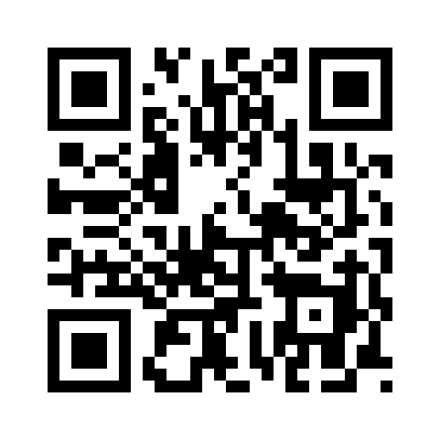
\includegraphics[width=0.4\textwidth]{img/qr-code.png} 
%\captionsetup{justification=centering}
\caption{QR Code \cite{QRcodefo71online}}
%public domain
\label{img:qr-code}
\end{figure}

Location-based AR used GPS\footnote{Global Position System.} coordinates and can be used together with marker tracking to create AR experiences that can be seen around the world through a browser on a phone. AR.js is completely open source and licensed under the \href{https://mit-license.org/}{MIT License}. The library works on any phone with WebGL and WebRTC. There are two builds for this project, one which works with \textit{three.js} and another that works with \textit{A-FRAME}. Both of these platforms will be discussed in Section \ref{subsubsec:webvr}. 

\paragraph{WebGL}

\paragraph{WebRTC}

\subsubsection{WebVR}\label{subsubsec:webvr}

\todo[inline]{WebGL frameworks: three.js, babylon.js, and PlayCanvas. WebXR frameworks: A-Frame and ReactVR. (https://immersive-web.github.io/webxr-samples/explainer.html) }

\subsubsection{WebVR Audio}

Ambisonics has clear bandwidth efficiencies over \textit{Object Based Audio} (OBA) solutions due to the fact the $N$ sources can be encoded into a lower number of channels, dubbed ambisonic harmonics, and then decoded binaurally. This sound-field synthesis technique varies in quality depending on the order of the ambisonic system. A FOA system might reduce the amount of data required to represent a sound field, but a HOA might provide a more realistic experience given the improved spatial resolution of the system.

There is a key trade-off here that must be reconciled in order to determine what is the minimum number of ambisonic channels that are required for a suitable XR experience. In addition to this criterion, we must also consider that a number of high-quality data compression ambisonic systems are able to further reduce this data load at the expense of quality of experience (QoE). 

The data compression algorithms use perceptual features of the auditory system to reduce the amount of data required for satisfying playback. Among these algorithms, the MP3 system is perhaps the most familiar to consumers. MP3 is not well suited for spatial audio, however other compression systems exist for this task. These compression systems exploit our ear's inability to hear tones below a certain \textit{masking threshold}. When we hear a tone a narrow region of our \textit{basilar membrane} gets activated. It has been shown that when two tones, both inside this region, are played together, if one is not sufficiently loud, it will not be perceived at all. This is only one of various mechanisms artfully exploited by compression systems. Herre \cite{herre2015mpeg} provides a good overview of multi-channel data compression systems which informed the design of MPEG-H - one of the more popular CODECs for spatial audio.

Three minutes of uncompressed audio at 44,100 samples per second, and 24 bits per sample, results in roughly 2.2GB of audio data at 9OA. In contrast a 3OA system would result in 6 times less amount of space required - with only 0.35GB of data required to reproduce the sound field. A FOA file, with 3 minutes of music, would only require roughly 0.09GB of data\footnote{Or 90MB.}. The size of the music file is an important bottleneck in these types of works. In cases where sound is transmitted live in an ambisonic format it is also important to determine the \textit{bit-rate} of the audio stream. This is the amount of data per unit time - generally seconds - that is required for proper reproduction. 

In order to perform the binaural synthesis required for immersive \textit{Virtual Auditory Environments} (VAE) recreation, WebXR frameworks must perform multiple convolutions with HRIRs. Convolution, even in the frequency domain, is a CPU intensive operation. In a "virtual speaker" approach to binaural decoding, two convolutions are needed for each virtual speaker. The number of virtual speakers will affect the \textit{Quality of Experience} (QoE), thus a balance needs to once more been struck, this time between high "virtual speaker" count and low-CPU requirements. 

\paragraph{Resonance}

There are several implementations of binaural spatial audio online. Among them, the most popular open-source solution is Resonance. In \cite{gorzel2019efficient}, Gorzel describes some techniques to optimize HOA playback. Firstly, the author describes the implementation of a Look Up Table (LUT) instead of using $cos$ or $sin$ functions inside ones code. This way the spherical harmonic coefficients are pre-computed and can be retrieved based on the current angles of the sound source. In order to provide smooth transitions between coefficients well known interpolation schemes can be used. More importantly, however, this paper points out the possibility of exploiting spherical harmonic symmetries in order to reduce the memory requirements of the system. Gorzel points out that spherical harmonics have well-known symmetries making it possible to derive all coefficient from a single quadrant determined by the azimuth and elevation angle of the sound source. By simply calculating the front-left-top quadrant of the sphere, all the other values can be known by simply applying sign changes. 

Another optimization undertaken by the authors involves reducing the number of convolutions required for binaural synthesis by assuming left/right hemispherical symmetry. Consider a sound source at 45\textdegree to the left of the subject with an elevation of 0\textdegree. If we were to simply swap the left and right channels then in essence it would be like presenting the sound source at 45\textdegree to the right of the subject. Of course, this assumes that the head is exactly symmetrical, which is not true. Further studies are required to see if these optimizations degrade the sound quality of the renderer in a substantive fashion. Another small optimization is the use of a single HRIR for sources with azimuth 0. Since the left and right channel are assumed to be symmetric, a single convolution is needed to process these sources. 

Gorzel et al. also use spherical domain representations of the SADIE HRTF data-set in lieu of the traditional virtual speaker approach in order to reduce the number of convolutions required. In this approach a decoding matrix is constructed based on the positions of the IRs, much like in normal virtual speaker approach. A matrix of impulse responses, corresponding to the same directions, is then multiplied by this matrix, which effectively encodes the IRs into the spherical domain. The decoding matrix is found by finding the \textit{Moore-Penrose pseudo-inverse} of the matrix $L$ defined in Equation \ref{eq:re-enc-mat}. 

\begin{equation}
\mathbf{L}=\left[\begin{array}{cccc}
Y_{0}^{0}\left(\Phi_{1}, \Theta_{1}\right) & Y_{0}^{0}\left(\Phi_{i}, \Theta_{i}\right) & \ldots & Y_{0}^{0}\left(\Phi_{N}, \Theta_{N}\right) \\
Y_{1}^{-1}\left(\Phi_{1}, \Theta_{1}\right) & Y_{1}^{-1}\left(\Phi_{i}, \Theta_{i}\right) & \ldots & Y_{1}^{-1}\left(\Phi_{N}, \Theta_{N}\right) \\
\vdots & \vdots & \vdots & \vdots \\
Y_{n}^{m}\left(\Phi_{1}, \Theta_{1}\right) & Y_{n}^{m}\left(\Phi_{i}, \Theta_{i}\right) & \ldots & Y_{n}^{m}\left(\Phi_{N}, \Theta_{N}\right)
\end{array}\right]
\label{eq:re-enc-mat}
\end{equation}

\todo[inline]{Describe Moore-Penrose pseudo-inverse.}

The result is a matrix with $(N=1)^2$ columns and an arbitrary number of filter coefficients, which can directly be convolved with the B-Format ambisonics spherical harmonics. In the case of a 3OA signal and a 26-point Lebedev grid the number of convolutions is reduced from 26 to 16 (\~62\% reduction). An added benefit of this method is that any \textit{shelf-filtering}, such as a \textit{MaxRe} shelf-filtering, can be done offline, prior to the decoding stage. This reduces the required amount of CPU and improves speed on low-end mobile devices \cite{gorzel2019efficient}.

\todo[inline]{Describe Lebedev grid.}

In addition to all these optimizations Resonance also has methods for controlling the sound source spread, simulation of near-field sources, and, specialized reverbs which simulate different room effects. One of the contributions the authors suggest is allowing for personalized HRTFs. The source code includes MATLAB and C++ code and the Github repository shows how to build these components to target different platforms making it highly flexible. The code is open-source and licensed under Apache 2.0. 

\todo[inline]{Consider breaking into paragraphs?}

\paragraph{Pluggy}

\paragraph{JSAmbisonics}

Politis et al. \cite{politis2016jsambisonics} describe another implementation of an open-source webVR solution in their 2016 publication. The authors present an ambisonic library built using the Web Audio API (WAA), written in JavaScript (JS), for interactive spatial audio rendering. It supports HOA and implements the most fundamental processing blocks for generating and reproducing sound scenes, such as rotations and binaural decoding. In the next paragraphs we will provide more detail regarding these transforms. 

\subparagraph{Ambisonic Rotation}

Ambisonic rotation is an integral part of any binaural ambisonic system. This operation allows the sound to change dynamically in response to users' head movements. Ambisonic rotation in FOA is trivial and reduces to the following equations in $\mathbb{R}^{3}$ \cite{kronlachner2014spatial}\footnote{We opt for $\alpha, \beta, \gamma$ to avoid confusion between rotation angles and ambisonic panning angles. Note also that here we are referring to a sound-field rotation after encoding.}. 

$R_z$ defines the counterclockwise rotation matrix about the z-axis.

\begin{equation}
R_{z}(\alpha)=\left(\begin{array}{ccc}
\cos \alpha & -\sin \alpha & 0 \\
\sin \alpha & \cos \alpha & 0 \\
0 & 0 & 1
\end{array}\right)
\end{equation}

$R_y$ defines the counterclockwise rotation matrix about the y-axis.

\begin{equation}
R_{y}(\beta)=\left(\begin{array}{ccc}
\cos \beta & 0 & \sin \beta \\
0 & 1 & 0 \\
-\sin \beta & 0 & \cos \beta
\end{array}\right)
\end{equation}

$R_x$ defines the counterclockwise rotation matrix about the x-axis.

\begin{equation}
R_{x}(\gamma)=\left(\begin{array}{ccc}
1 & 0 & 0 \\
0 & \cos \gamma & -\sin \gamma \\
0 & \sin \gamma & \cos \gamma
\end{array}\right)
\end{equation}

The letters $\alpha, \beta, \gamma$ correspond the to the \textit{yaw}, \textit{pitch} and \textit{roll} angles respectively. The coordinate system for these matrices has the x-axis pointing towards the front, the y-axis pointing towards the left, and the z-axis pointing to the right. When multiplying your signal matrix, the order will also affect the results. In this case, the signals should be ordered $[x, y, z]$, and then re-ordered if necessary\footnote{Rotating the 0th order harmonic has no effect.}. These three rotation matrices can also be combined into a single larger matrix by multiplying them together. Note that the order in which these transforms are combined is important, the convention we will use is roll, pitch, yaw. The combined formula, resulting from multiplying these three matrices in this order yields:

\begin{equation}
\begin{array}{l}
R(\alpha, \beta, \gamma)=R_{z}(\alpha) R_{y}(\beta) R_{x}(\gamma)= \\
\left(\begin{array}{ccc}
\cos \alpha \cos \beta & \cos \alpha \sin \beta \sin \gamma-\sin \alpha \cos \gamma & \cos \alpha \sin \beta \cos \gamma+\sin \alpha \sin \gamma \\
\sin \alpha \cos \beta & \sin \alpha \sin \beta \sin \gamma+\cos \alpha \cos \gamma & \sin \alpha \sin \beta \cos \gamma-\cos \alpha \sin \gamma \\
-\sin \beta & \cos \beta \sin \gamma & \cos \beta \cos \gamma
\end{array}\right)
\end{array}
\end{equation}

Finally, care should be given to understand the direction of rotation. Counter-intuitively, what we seek is for the ambisonic rotation to compensate for the listener's head movement. Picture a sound source at 45\textdegree. If the user moves his or her head 45\textdegree clockwise, from their perspective, the source will remain at 45\textdegree, while it should actually now be at 0\textdegree. Thus, the clockwise rotation of the user, should result in a counterclockwise ambisonic rotation. 

Rotations in $\mathbb{R}^{4}$ and above are more complicated but necessary to move beyond FOA. There are two common methods used to accomplish this task. One involves computing a single higher order rotation of $\pm90\textdegree$ in $R_{y}$. $R_{z}$ rotation matrices of higher order are relatively easy to compute. Kronlachner's thesis shows the following derivation of this matrix up to second order.

\begin{equation}
\boldsymbol{R}_z(\alpha)=\left(\begin{array}{c|ccc|ccccc|cc}
1 & 0 & 0 & 0 & 0 & 0 & 0 & 0 & 0 & \mathbf{0} & \\
\hline 0 & \cos \alpha & 0 & \sin \alpha & 0 & 0 & 0 & 0 & 0 & \\
0 & 0 & 1 & 0 & 0 & 0 & 0 & 0 & 0 & \mathbf{0} & \\
0 & -\sin \alpha & 0 & \cos \alpha & 0 & 0 & 0 & 0 & 0 & & \\
\hline 0 & 0 & 0 & 0 & \cos 2 \alpha & 0 & 0 & 0 & \sin 2 \alpha & & \\
0 & 0 & 0 & 0 & 0 & \cos \alpha & 0 & \sin \alpha & 0 & \\
0 & 0 & 0 & 0 & 0 & 0 & 1 & 0 & 0 & \mathbf{0} & \\
0 & 0 & 0 & 0 & 0 & -\sin \alpha & 0 & \cos \alpha & 0 & & \\
0 & 0 & 0 & 0 & -\sin 2 \alpha & 0 & 0 & 0 & \cos 2 \alpha & & \\
\hline \mathbf{0} & & \mathbf{0} & & & & \mathbf{0} & & & \cos 3 \alpha & \\
 & & & & & & & & & & \ddots
\end{array}\right)
\end{equation}

Kronlachner's technique, adopted from Zotter's work, involves using a single $R_{y}$ rotation matrix to position the spherical harmonic for variable rotation using the more easily computable $R_{z}$ matrix, and later using a second $R_{y}$ rotation of 90\textdegree, to return the harmonic to its original state. These 90\textdegree rotation matrices can be found at IEM's website\footnote{\href{https://ambisonics.iem.at/xchange/fileformat/docs/spherical-harmonics-rotation}{Site} accessed April 1, 2021.}

\todo[inline]{I don't quite understand how this works. I will try to ask Justin to explain.}

Politis \cite{politis2016jsambisonics}, and a number of other authors, instead compute all rotation matrices using a recursive algorithm. Spherical harmonics are not only found in the audio domain, but are pertinent in chemistry, physics, and mechanics. The rotation matrices derived in Politis's work come originally from Ivanic and Ruedenberg's paper in "The Journal of Physical Chemistry" \cite{ivanic1996rotation}. 
The details of these calculations are outside the scope of this chapter. However, implementations of these formulas can be found in Politis's Spherical Harmonic Transform (SHT) library. Politis has implemented these formulas both in JS and in MATLAB. Gorzel et al. \cite{gorzel2019efficient} have implemented these in numerous other computer languages. For those wishing to write these from scratch we recommend the paper by Blanco et al. \cite{blanco1997evaluation} which contains pseudo-code and easy to understand formulations. 

\subparagraph{Ambisonic Reflection}

Reflection is a simple operation in the ambisonic domain given the symmetry of spherical harmonics. Reflection, or mirroring, refers to the ability to rotate the sound-field 180\textdegree along any of the three coordinate planes (yz, xz, or xy). This simplifies to polarity changes of specific harmonics, based on whether they are symmetric or anti-symmetric\footnote{All harmonics are one or the other.}. Politis provides Equation \ref{eq:ambi-reflect} to accomplish this task.

\begin{equation}
\begin{aligned}
(m<0 \wedge m \text { even }) \cup(m \geq 0 \wedge m \text { odd }):  \mathbf{y z}\\
m<0: \mathbf{x z}\\
(n+m) \text { odd }: \mathbf{x y} 
\end{aligned}
\label{eq:ambi-reflect}
\end{equation}

This might be desired, for example, if a microphone is suspended from the ceiling in a concert hall, and we now wish to use the recording in a more traditional orientation. For each case when the desired harmonics are found a multiplication by -1 results in a change of polarity, giving us our desired result. In other words:

\begin{enumerate}
    \item For rotation about the \textbf{yz} plane, we must find all harmonics with ambisonic degree $m$ that are smaller than 0 and even, as well as those that are greater than or equal to 0 and odd. This is a front-back flip.
    \item For a rotation about the \textbf{xz} plane, we must find the harmonics that have ambisonic degree $m$ smaller than 0.  This is a left-right flip.
    \item For a rotation about the \textbf{xy} plane, we must find the harmonics where the sum or ambisonic degree $n$ and $m$ is odd.  This is a up-down flip.
\end{enumerate}

\subparagraph{Ambisonic Beam-forming}

Beam-forming refers to the ability of steering an audio signal, either at the capture or reproduction stage, by using a series of delays and gain adjustments. In the spherical harmonic domain it is possible to create adjustable \textit{virtual microphones} pointing in arbitrary directions. This is useful when we want to isolate a particular sound inside the sound-field. It is also the basis of ambisonic decoding. Note that this transform results in a monophonic signal. These monophonic signals, however, can be re-encoded into the SH domain if need be, or used in more conventional stereo mix-downs.

\begin{equation}
x_{\mathrm{vm}}\left(t, \boldsymbol{\gamma}_{0}\right)=\mathbf{w}^{\mathrm{T}}\left(\boldsymbol{\gamma}_{0}\right) \mathbf{b}(t)
\label{eq:ambi-beamform}
\end{equation}

\noindent where
\begin{description}
\item  $\boldsymbol{\gamma}_{0}$ corresponds to the orientation of the virtual microphone,
\item  $\mathbf{w}(\gamma_{0})$ corresponds to the $(N+1)^{2}$ vector of beam-forming weights, and,
\item  $\mathbf{b}(t)$ corresponds to the ambisonic spherical harmonics, otherwise known as B-format signals (at time $t$). Using vector notation to denote a block size of 1.
\end{description}

\todo[inline]{use this format for all equation where listing variable. using the begin description command.}

Equation \ref{eq:ambi-beamform} shows the equation provided by Politis \cite{politis2016jsambisonics} for this task. The library allows for various different types of microphone patterns with different front/back \textit{rejection ratios}\footnote{Measure of how much sound incident from the front is captured relative to sound incident from behind.}. Politis \cite{politis2016jsambisonics} provides additional equations for the derivation of specific polar patterns including: \textit{cardioid}, \textit{hypercardioid} and a \textit{max-rE} which "maximizes the acoustic intensity vector in an isotropic diffuse field." The max-rE derivation comes from the decoding literature. The $\mathbf{b}(t)$ term is obtained by taking the outer product of your original source signal and the vector $\mathbf{y}$ of \textit{spherical harmonic coefficients} described by Equation \ref{eq:r-sph-harm}.

If the two vectors have dimensions $n$ and $m$, then their outer product is an $n$ by $m$ matrix\footnote{$n$ and $m$ here should not be confused with indices for spherical harmonics. These values refer instead to the rows and columns of the product $\mathbf{B}$}. The outer product is defined as: 

\begin{equation}
\mathbf{s} \otimes \mathbf{y}=\mathbf{B}=\left[\begin{array}{cccc}
s_{1} y_{1} & s_{1} y_{2} & \ldots & s_{1} y_{n} \\
s_{2} y_{1} & s_{2} y_{2} & \ldots & s_{2} y_{n} \\
\vdots & \vdots & \ddots & \vdots \\
s_{m} y_{1} & s_{m} y_{2} & \ldots & s_{m} y_{n}
\end{array}\right]
\end{equation}

\paragraph{Web Audio API}

\paragraph{HOAST}

Deppisch et al. \cite{deppisch2020hoast} in 2020 published a paper describing the development of a Higher Order Ambisonic STreaming platform (HOAST). This collaboration between IEM, Aalto, Hofer Web Solutions and Zylia resulted in an open source\footnote{GNU GPLv3 licencese.} web player for 360\textdegree  video and HOA. As the authors noted, most video players for this type of media only allow up to 2OA; most, in fact, only support FOA. The goal of this project was to create a video player capable of outputting up to 4OA with an associated VR video. 

HOAST is built upon the already existing Web Audio API, which is compatible with most modern browsers. One of the problems with these systems is that despite their superior flexibility, there are still only certain browsers, in certain configurations, that support this type of media. Luckily, all the browsers are free to install and use. In the case of HOAST, Firefox and Chromium-based browsers are recommended. An additional issue is that, due to the infancy of this technology, there are still programming changes happening routinely, which means maintenance and support is required to maintain these applications operational. Deppisch et al., for example, describe the deprecation of \textit{ScriptProcessorNodes} for \textit{AudioWorklets}, which despite their superiority can cause glitches on some devices. 

Another issue with HOAST, or any 360\textdegree video player with HOA for that matter, is the need of a large amount of data and processing power for a proper experience. This means that HOAST, as other players, might work well in some mobile devices but not all. They might also work relatively well on a laptop device but these do not provide as immersive an experience as HMDs. HOAST does however work on native VR HMDs such as on an Oculus Rift or an HTC Vive. 

The Web Audio API\footnote{Application Programming Interface.} also has limits on the number of audio channels that it supports for audio nodes. According to the authors of HOAST: "all Web Audio API implementations establish a 32-channel limit". This in turn limits the Ambisonic audio to 4OA, which requires 25 channels. 

\subparagraph{CODECs, Container, and Signal Flow}

In order to provide reasonable small file sizes a number of different compression algorithms were evaluated by Deppisch et al. The OPUS CODEC is one of the preferred compression systems for ambisonic audio on the web, given it's large channel count and open-source nature. Some other popular file types which allow for multi-channel audio files include: WAV, FLAC, AAC, and VORBIS. All major browsers support the OPUS codec, with the exclusion of Apple's Safari Browser (version 13.1). 

After an audio CODEC is selected, the next step was to determine which streaming platform would be adopted. The authors in this case used MPEG-DASH player was selected due to it being codec-agnostic. MPEG-DASH is an \textit{adaptive streaming technology} which automatically adjusts media quality based on the uses available bandwidth to ensure smooth playback. The VP9 video CODEC\footnote{https://en.wikipedia.org/wiki/VP9} was also selected and the WebM container\footnote{https://en.wikipedia.org/wiki/WebM} for combining both audio and video. The actual ambisonic manipulation in JavaScript is accomplished using the JSAmbisonics implementation by Politis et al \cite{politis2016jsambisonics}.

Figure \ref{fig:hoast-sig-flow} shows the signal flow of HOAST. 4OA files, encoded with OPUS, are packaged in WebM and streamed using MPEG-DASH. On the client side, the DASH stream is received via dash.js and sent to an HTML \textit{audio element}. The OPUS decoded audio signals from the HTML audio element are then passed to the Web Audio API's \textit{audio context} via a \texttt{MediaElementAudioSourceNode}. These are then passed to custom processing nodes from JSAmbisonics \cite{politis2016jsambisonics} which perform the rotation and zoom based on the user's FOV. Finally, the Web Audio API convolver nodes are used for binaural decoding. The final two signals are sent to the \texttt{AudioDestinationNode}, the last node in the signal path, preceding the user. 

\begin{figure}[ht!]%force figure here, top, strict
\centering
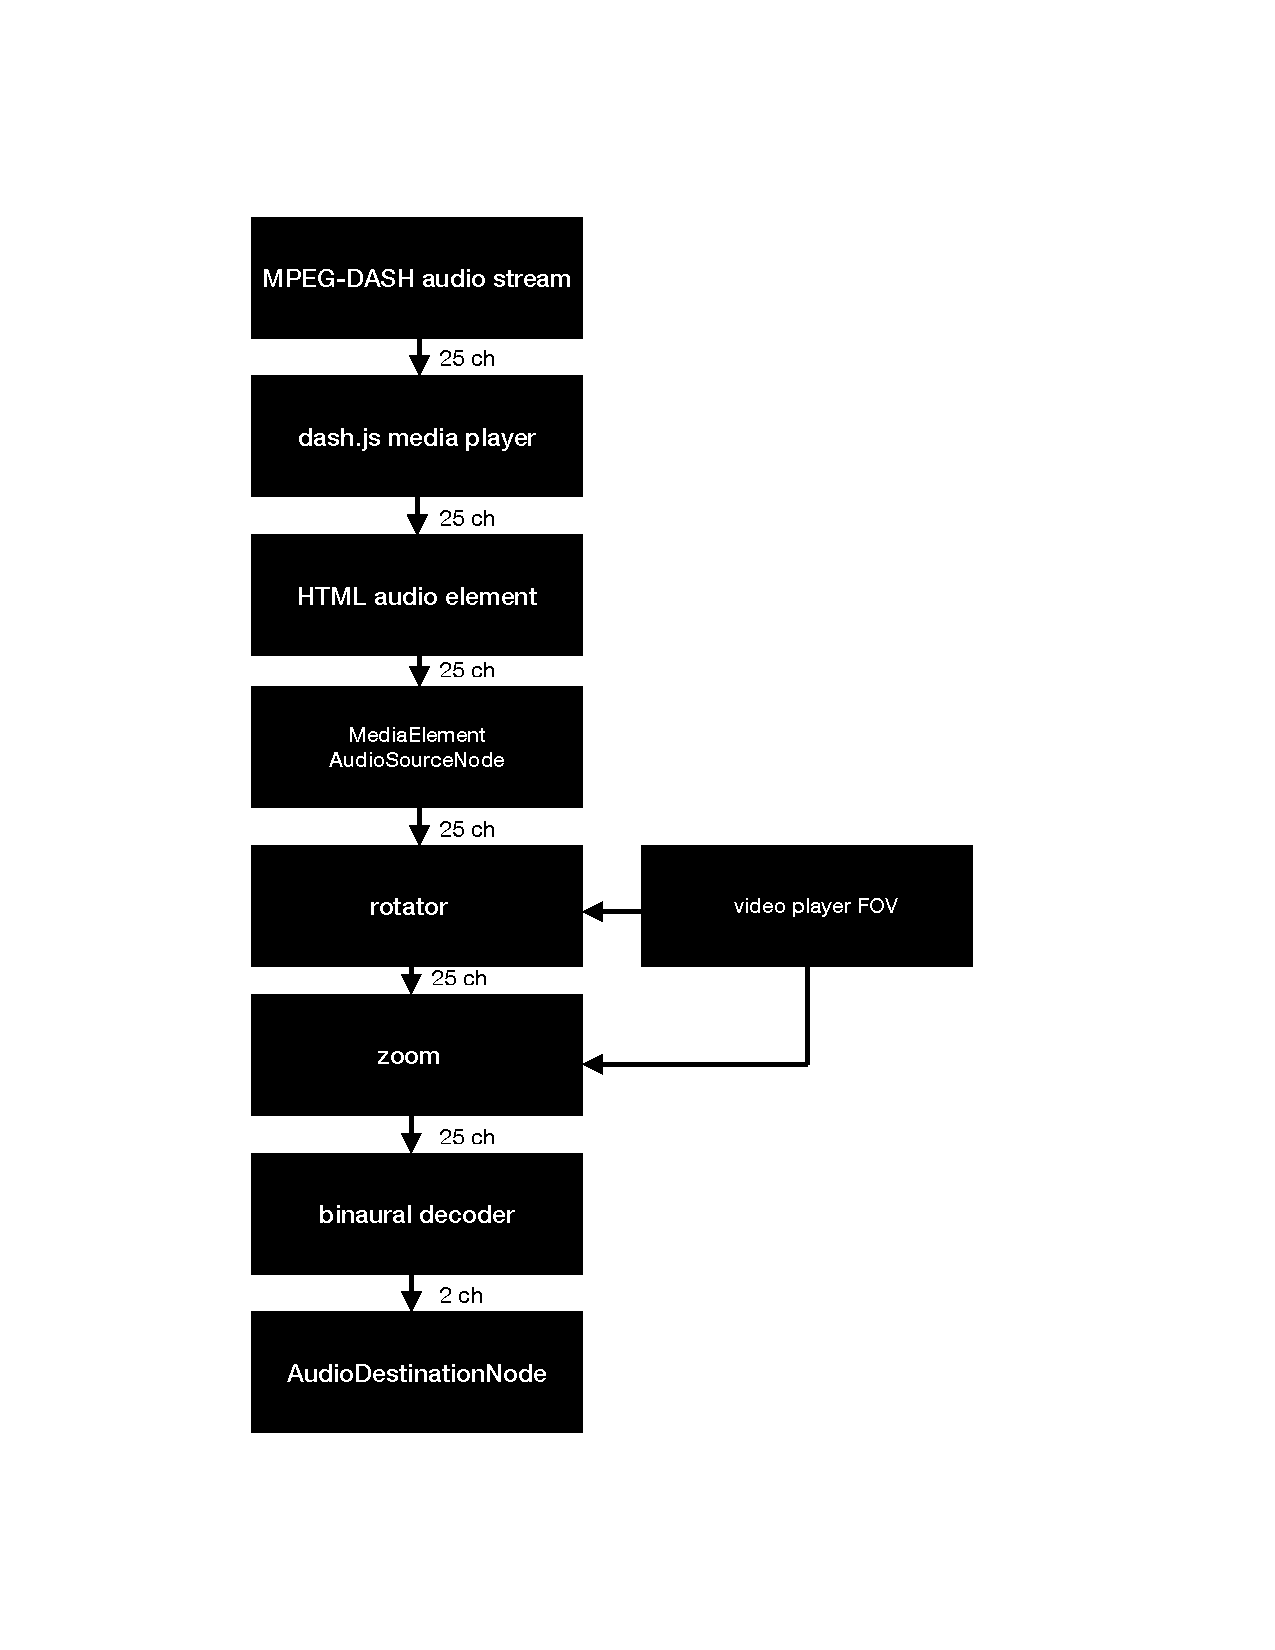
\includegraphics[width=0.9\textwidth]{img/hoast-sig-flow.pdf} 
%\captionsetup{justification=centering}
\caption{HOAST Signal Flow}
\label{fig:hoast-sig-flow}
\end{figure}

Ambisonic zoom is outside the scope of what we wish to cover here, but details about it can be found in the Appendix \ref{ch:appendix-math} under Section \ref{sec:ambi-zoom}. In the next paragraphs we will continue discussing the decoding scheme used, video rendering, and website implementation of HOAST.

\subparagraph{Binaural Decoding}

The \textit{binaural decoding} implemented in HOAST does not involve the traditional \textit{virtual loudspeaker} approach\footnote{As a reminder: in the virtual loudspeaker system, linear combinations of ambisonic harmonics are used to create speaker feeds, identically to ambisonic decoding. The resulting feeds are convolved with HRTFs in the direction of the virtual speaker.}. Instead, the HOAST binaural decoder are based on the solution to a \textit{Least Squares} (LS) problem which results in decoding filters. Deppisch et al. provide the following equation:

\begin{equation}
\omega_{\mathrm{LS}}=\arg \min _{\omega}\left\|\boldsymbol{Y}_{\Upsilon} \boldsymbol{\omega}-\boldsymbol{h}_{\Upsilon}\right\|_{2}^{2}
\label{eq:ls-bin-dec}
\end{equation}

The $(N+1)^2$ decoding filters\footnote{Recall that $N$ refers to the ambisonic order. So we will have a single filter for each ambisonic harmonic.} $\omega_{\mathrm{LS}}$ will minimize the least squares error between HRTF measurements in $\boldsymbol{h}_{\Upsilon}$ and the spherical harmonics in $\boldsymbol{Y}_{\Upsilon}$ evaluated at all HRTF directions in the measurement grid $\Upsilon$ \cite{deppisch2020hoast}. In this case a Lebedev grid\footnote{See appendix} of HRTF measurements is used, and in order to improve the perceptual decoding of binaural signals, the magnitude least squares (MagLS) approach is used. For low frequencies, a LS solution is applied. For reference Equation \ref{eq:arg-min} shows the definition of the $\arg \min$ operator. 

\begin{equation}
\underset{x \in S}{\arg \min } f(x):=\{x \in S: f(s) \geq f(x) \text { for all } s \in S\}
\label{eq:arg-min}
\end{equation}

are points $x$ for which $f(x)$ attains its smallest value. The L2 norm, also used Equation \ref{eq:ls-bin-dec}, is defined as:

\begin{equation}
\|\boldsymbol{x}\|_{2}:=\sqrt{x_{1}^{2}+\cdots+x_{n}^{2}}
\end{equation}

The original set used to generate these filters had $P=2702$ HRTF measurements. The goal of this algorithm is to reduce this to 25 filters for the left ear, and 25 filters for the right (4OA). This is similar to the Resonance architecture \cite{gorzel2019efficient} which accomplishes significant reduction of data using an equivalent approach. A common use of the pseudo-inverse is to computer the LS solution to a system of linear equations. Schorkhuber et al. \cite{schorkhuber2018binaural} discusses in greater detail optimizations to the LS approach to binaural rendering. 

In addition to this LS optimization, the authors also describe the use of a FOA impulse response, generated using the Image Source Method (ISM), in order to improve externalization. This ISM impulse response is applied only to the first-order\footnote{W, Y, Z, X harmonics in ACN ordering, namely.} decoding filters to reduce latency. The length of the higher-order decoding filters is 256 samples. The ISM is a technique that can be used to generate synthetic room impulse responses \cite{allen1979image}\footnote{Detailed discussion of this technique is outside the scope of this chapter.}. 

\subparagraph{Video Rendering}

In order to display 360\textdegree video along with the ambisonic audio, Video.js was used in combination with the videojs-contrib-dash plug-in \cite{deppisch2020hoast}. This allowed the authors to receive and play back MPEG-DASH audio/video streams while supporting equirectangular video\footnote{Equirectangular projection is a typical transform used to display 360 degree content in 2D.} via a custom made plug-in called videojs-xr, which is an update to the pre-existing videojs-vr relying on the newer WebXR API. A polyfill\footnote{Polyfill is a library that: injects an XR implementation into a browser if one does not exist, patches browsers that have incomplete implementations of the API, and, provides a synthesized VR display when WebXR is not supported.} makes HMDs usable in Firefox and Chromium-based browsers. In Chromium-based browsers enabling the \textit{\#webxr} flag, setting the \textit{\#webxr-runtime} and disabling \textit{\#xr-sandbox} might be required.

\subparagraph{Website Implementation}

On the backend side the HOAST web application allows basic CRUD (Create, Read, Update, Delete) tasks of the data. The database holds two main types of data: the meta data of the media files, and, the information related to the "channel" owner (ie. IEM channel). The python-based web framework Django was used, while for the front end the Bootstrap toolkit was used. Currently\footnote{Written in March 2021.} only the creators are allowed to manage the data but the code is freely available so anyone is capable of loading it unto a new server to start their own library. One could also add a more complex backend allowing any user to create their own "channel", but this has not yet been implemented.

% https://immersive-web.github.io/webxr-samples/explainer.html

%https://www.khronos.org/gltf/

% Most usage of WebGL today happens via frameworks that significantly simplify the creation of 3D scenes compared to using raw WebGL. Some of the more popular examples are three.js, babylon.js, and PlayCanvas. There's also frameworks that are specifically designed to create XR content on the web, such as A-Frame and ReactVR. These are all fantastic libraries with their own strengths and focuses, and in general it's recommended that you find tools that suit your needs and rely on them rather than trying to build your own rendering systems from scratch.

% However, most frameworks will also hide away the details of interacting with the WebXR API. That's generally great for users, but not terribly useful when the entire point of your code is to demonstrate how to use the API! At the same time, we don't want the WebXR logic to be obscured by hundreds of lines of WebGL calls. As a result, these samples make use of their own minimalistic rendering library that is specifically designed to highlight use of the WebXR API and de-emphasize the WebGL rendering logic. It is not recommended that you use this library in your own projects, as you will almost certainly be better served by one of the more popular, better established frameworks.

\todo[inline]{Simultaneous Localization and Mapping (SLAM), 360 cameras, matched zone, locomotion}


\section{Open XR Tools}

\section{The Philosophy of "Public Domain"}

\todo[inline]{might move this section to earlier part.}

% Given our focus on the use of FOSS. 

Technology has been an important part of art-making for many decades now. With the decreasing cost of computers, and their improved potential, more people today are capable of making art with computers than ever before. The technology industry remains focused on: improving, updating, and refining its products; in order to generate profit. Unfortunately, these systems are often designed with the latest hardware and operating systems in mind, which places an economic burden on composers and musicians. Furthermore, many popular exhibits and artistic works today feature technology as a core feature of the material, which excludes those who lack access or the skills to create such content.

Software, like digital art, poses a complex economic problem. Unlike physical objects, or direct services, software and digital art can easily be duplicated at little to no cost. Intellectual Property (IP) lies at the heart of this problem as was addressed by Puckette in \cite{puckette2004owns}. In his paper, Puckette used Pure Data (Pd) as a case study of what happens when a research institution commercializes its research. In the article, Puckette argues that IRCAM's\footnote{Institut de Recherche et Coordination Acoustique/Musique.} decision to enforce its IP claims to Pd and sell it as MAX/MSP resulted in a noted drop in the credibility of the institution as a research facility. The name Pd also means Public Domain. Drawing these IP lines is anything but simple since most valuable research draws from other authors' work. Similarly, most worthwhile artworks draw inspiration from its predecessors or contemporaries.

Much like software, digital art can be difficult to price. A physical painting can be analyzed to its authenticity and a price can be set based on what the market is willing to pay for it. A digital sound file, on the other hand, can be duplicated nearly for free, and mass distribution is just as cheap. A musical score operates on basically the same principle. \cite{puckette2001new} explored the idea of bringing some seminal computer music works into the public domain by using Pd, however, not all the works are included on his website, because IRCAM insisted some of patches be taken down. This creates an interesting dilemma for the composers, who naturally would prefer their music be performed as often as possible. 

When working in the scientific domain, one of the applied principles for validating experiments is the reproduction of the research. One of the benefits of using public domain tools, like Pd, is the ability to exercise a similar principle in the artistic domain. The idea being that aesthetic musical principles are hard to extend if the technology inherent to them is proprietary. In the pedagogical domain, this idea is also extremely powerful. Using public domain tools enables one to share their teachings with a wider subset of the population, without having to consider the economic barriers that software can sometimes create. 

Fernando Lopez-Lezcano, a composer and computer scientist at Stanford, has also been interested in this dichotomy for a long time. Fernando has been building Linux distributions for sound research at CCRMA for many years now. In \cite{CEC-eCon28-online} Fernando talks about the traditions established at Stanford related to open source software and how these have evolved over the years. 

%https://econtact.ca/11_3/index.html
%https://econtact.ca/11_3/lopez_lezcano_ccrma.html

\section{The Future of XR}
\section{Conclusion}

%conclusion
\chapter{Conclusion}\label{ch:conclusion}
 
It is entirely likely that different subsections will have to be moved around. I am still trying to come up with the best way to organize the thesis.
  
\section{A section}
Lorem ipsum dolor sit amet, consectetuer adipiscing elit. Nulla odio
sem, bibendum ut, aliquam ac, facilisis id, tellus. Nam posuere pede
sit amet ipsum. Etiam dolor. In sodales eros quis pede.  Quisque sed
nulla et ligula vulputate lacinia. In venenatis, ligula id semper
feugiat, ligula odio adipiscing libero, eget mollis nunc erat id orci.
Nullam ante dolor, rutrum eget, vestibulum euismod, pulvinar at, nibh.
In sapien. Quisque ut arcu. Suspendisse potenti. Cras consequat cursus
nulla.

\subsection{A subsection}
Lorem ipsum dolor sit amet, consectetuer adipiscing elit. Nulla odio
sem, bibendum ut, aliquam ac, facilisis id, tellus. Nam posuere pede
sit amet ipsum. Etiam dolor. In sodales eros quis pede.  Quisque sed
nulla et ligula vulputate lacinia. In venenatis, ligula id semper
feugiat, ligula odio adipiscing libero, eget mollis nunc erat id orci.
Nullam ante dolor, rutrum eget, vestibulum euismod, pulvinar at, nibh.
In sapien. Quisque ut arcu. Suspendisse potenti. Cras consequat cursus
nulla.

\appendix

\chapter{Mathematics}
%a1 

\section{Coordinate System}
\section{Spherical Bessel Functions of the First Kind}
\section{Spherical Harmonics}
\section{Associate Legendre Functions}
\section{Spatial Soundfield Decomposition}

% A soundfield within a source free region of space at a point $(r, \theta, \phi)$ with respect to an origin $O$ of the spherical coordinate system can be written as:

% \begin{equation}
% P(r, \theta, \phi, k)=\sum_{n=0}^{\infty} \sum_{m=-n}^{n} C_{n m}(k) j_{n}(k r) Y_{n m}(\theta, \phi)
% \end{equation} 

% where $C_{n m}(k)$ are soundfield coefficients, $k=2 \pi f / c$ is the wave number, $f$ is the frequency, $c$ is the speed of sound propagation, $j_{n}(k r)$ is the $n$th order spherical Bessel function of the first kind, $Y_{n m}(\theta, \phi)$ are the spherical harmonics, defined by

% \begin{equation}
% Y_{n m}(\theta, \phi)=\mathcal{P}_{n|m|}(\cos \theta) E_{m}(\phi)
% \end{equation}

% where
% $$
% \mathcal{P}_{n|m|}(\cos \theta) \triangleq \sqrt{\frac{(2 n+1)}{4 \pi} \frac{(n-|m|) !}{(n+|m|) !}} P_{n|m|}(\cos \theta)
% $$
% and
% $$
% E_{m}(\phi) \triangleq(1 / \sqrt{2 \pi}) e^{j m \phi}
% $$

% are the normalized associated Legendre functions and normalized exponential functions, respectively; $P_{n|m|}(\cos \theta)$ are the associated Legendre functions.

% For the case of soundfields, $P(r, \theta, \phi, k)$ is the pressure at a point as a function of frequency (wavenumber). The problem of soundfield acquisition is to extract the soundfield coefficients $C_{n m}(k)$ by sampling the soundfield over space and time. 

% \cite{chen2015theory} 


%appendix for scores (figures) related to ch1
\chapter{Mathematics} \label{ch:appendix-math}
%a2 - featured in chapter 3

\section{Coordinate System}

The selected coordinate system in this text, specially with regards to discussions regarding ambisonics has the x-axis pointing to the front, the y-axis to the left, and the z-axis to the top. The azimuth angle is denoted with the letter $\phi$ and the elevation angle is denoted with the letter $\theta$. 

$\phi$ increases counter-clockwise, contrary to our intuition. This is consistent with most ambisonic literature. The elevation $\theta$ increases upwards to +90\textdegree, which corresponds to the north pole, and decreases negatively to -90\textdegree, which corresponds to the south pole. 

A triplet, describing the direction of an ambisonic sound source, in Cartesian coordinates, is calculated in Equation \ref{eq:cartesian-triplet}. In order to convert this Cartesian representation to a polar representation we may use Equation \ref{eq:car2pol-ambi}

\begin{equation}
\boldsymbol{\theta}=\left(\begin{array}{l}
\theta_{x} \\
\theta_{y} \\
\theta_{z}
\end{array}\right)=\left(\begin{array}{c}
\cos \varphi \cos \vartheta \\
\sin \varphi \cos \vartheta \\
\sin \vartheta
\end{array}\right)
\label{eq:cartesian-triplet}
\end{equation}

\begin{equation}
\varphi=\arctan \frac{\theta_{y}}{\theta_{x}}, \quad \vartheta=\arctan \frac{\theta_{z}}{\sqrt{\theta_{x}^{2}+\theta_{y}^{2}}}
\label{eq:car2pol-ambi}
\end{equation}

\section{Spherical Bessel Functions of the First Kind}

\section{Spherical Harmonics}

\section{Associate Legendre Functions}

\section{Spatial Soundfield Decomposition}

\section{T-design}

\section{Ambisonic Zoom} \label{sec:ambi-zoom}

According to Deppisch \cite{deppisch2020hoast} ambisonic zoom is a combination of \textit{spatial windowing} and \textit{warping}. In the HOAST implementation, it is used to modify the soundfield in direct relation to video zooming. Namely, the ambisonic zoom and video are designed to work in conjunction seamlessly. 

In order to achieve this spatial transform the scene is decoded to a dense set of points. The points are weighted and changed in angle before re-encoding to ambisonics \cite{kronlachner2014plug}. More generally, in order to achieve the desired zoom, the ambisonic points need to be spread out if we wish to zoom in, and pushed closer together if we wish to zoom out. 

In HOAST \cite{deppisch2020hoast}, the transform matrices are computed in increments of 0.1 units for $\alpha$ ranging from 
$[1,2.5]$ where $\alpha = 1$ corresponds to a $ \pm 60^{\circ} $ FOV. Unfortunately, the authors do not specify which warping equation is used. The spatial windowing is also not specified by the authors. 

According to the author: "decoding the scene to the grid of t-design points with coordinates $\Theta_{P}$ spatial windowing using the diagonal matrix $G$ and re-encoding to the new points $\hat{\Theta}_{P}$ can be expressed as Equation \ref{eq:hoast-zoom}". 

\begin{equation}
\boldsymbol{T}(\alpha)=\boldsymbol{Y}\left(\hat{\boldsymbol{\Theta}}_{P}(\alpha)\right) \boldsymbol{G}(\alpha) \boldsymbol{Y}\left(\boldsymbol{\Theta}_{P}\right)^{\mathrm{T}}
\label{eq:hoast-zoom}
\end{equation}



Kronlachner (kronlachner-spat-transf-ambi.pdf) paper uses formula (27) which warps sound sources towards and away from the equator. Given abbreviations:

\begin{equation}
\begin{array}{ll}
\mu=\sin (\vartheta) & \text { original } \\
\tilde{\mu}=\sin (\tilde{\vartheta}) & \text { warped}
\end{array}
\end{equation}

\todo[inline]{Warping is complicated. I believe the way the HOAST paper does it is also different from other implementations.}

% A soundfield within a source free region of space at a point $(r, \theta, \phi)$ with respect to an origin $O$ of the spherical coordinate system can be written as:

% \begin{equation}
% P(r, \theta, \phi, k)=\sum_{n=0}^{\infty} \sum_{m=-n}^{n} C_{n m}(k) j_{n}(k r) Y_{n m}(\theta, \phi)
% \end{equation} 

% where $C_{n m}(k)$ are soundfield coefficients, $k=2 \pi f / c$ is the wave number, $f$ is the frequency, $c$ is the speed of sound propagation, $j_{n}(k r)$ is the $n$th order spherical Bessel function of the first kind, $Y_{n m}(\theta, \phi)$ are the spherical harmonics, defined by

% \begin{equation}
% Y_{n m}(\theta, \phi)=\mathcal{P}_{n|m|}(\cos \theta) E_{m}(\phi)
% \end{equation}

% where
% $$
% \mathcal{P}_{n|m|}(\cos \theta) \triangleq \sqrt{\frac{(2 n+1)}{4 \pi} \frac{(n-|m|) !}{(n+|m|) !}} P_{n|m|}(\cos \theta)
% $$
% and
% $$
% E_{m}(\phi) \triangleq(1 / \sqrt{2 \pi}) e^{j m \phi}
% $$

% are the normalized associated Legendre functions and normalized exponential functions, respectively; $P_{n|m|}(\cos \theta)$ are the associated Legendre functions.

% For the case of soundfields, $P(r, \theta, \phi, k)$ is the pressure at a point as a function of frequency (wavenumber). The problem of soundfield acquisition is to extract the soundfield coefficients $C_{n m}(k)$ by sampling the soundfield over space and time. 

% \cite{chen2015theory} 


%appendix for math (equations) related to ch2
\chapter{Code Listings}
%a3%appendix for cse (code) related to ch3

\chapter{Proposal 1: Spatial Music}
%This is my proposal for the work I would like to pursue over the next few years with Tom's support. It relates to chapter two of this paper. 

%This project fits with Rand's patch.

%%%%%%%%%%%%%%%%%%%%%%%%%%%%%%%%%%%%%%%%%%%%%%%%%%%%%%%%%%
%LIVE SPATIAL MUSIC%%%%%%%%%%%%%%%%%%%%%%%%%%%%%%%%%%%%%%%
%%%%%%%%%%%%%%%%%%%%%%%%%%%%%%%%%%%%%%%%%%%%%%%%%%%%%%%%%%

% abstract: 

% Over the last 20 years, we have seen an explosion in the number of spatial music works as a result of the increase of low-cost and high-quality computer processors on the market. In computer music, we see a number of works which feature acoustic instruments, as well as some pieces which are for computer only. This section will discuss the development of a spatial instruments which can be used for computer-only or electro-acoustic compositions [pool].

% intro:

% What are some typical ways that composers create spatial music for concert settings? What are the limitations of the computer-music systems? What are some instruments used in live settings for spatial music? What are some problems with these interfaces?

    %[to do]
    % Create a list of computer music tools that composers use to create live spatial music and describe them in detail.
    % Using the aforementioned list, explain some of the differences and similarities of these systems. 
    % Do the same with the spatial instruments.

% methodology:

% Propose a solution that overcomes the limitations of the aforementioned music systems. Describe the deficits and benefits of such a system. Do the same with one or more spatial instruments. 

% results: 
% discussion:

%%%%%%%%%%%%%%%%%%%%%%%%%%%%%%%%%%%%%%%%%%%%%%%%%%%%%%%%%%%%%%

% make use of: RPI, arduino, HCI, FOSS, DIY externals.

\section{Abstract}

Over the last few years a wide number of composers have began investigating the use of spatial audio in their compositions. The commercial growth of XR is perhaps one of the main reasons why we are seeing a newfound interest in these technologies. This proposal will deal with systems used by composers for creating spatial music including hardware and software solution. We are interested in solving some of the longstanding issues involved in the creation of spatial music. Furthermore, we are concerned with "future-proofing" these musical compositions to the greatest extent possible. We will also propose the development of a spatial instrument which will be used in the creation of one or more musical works.

\section{Introduction}
%topic/purpose, thesis statement

Over the last century a number of composers have explored the use of space as a key parameter in musical composition. Recently, with the growth of Extended Reality (XR), even more artists have began exploring this medium as a way to push the musical domain to new extremes. XR environments, such as Virtual Reality (VR) or Augmented Reality (AR), make up a new medium rich with creative possibilities for music-making. In this proposal, we would like to suggest the development of systems that can be used to perform live spatial music with the intention of pushing the boundaries of this domain in some significant way. 

In order to find gaps in the existing body of work, we offer in Chapter \ref{ch:spat-mus}, a substantive review of some of the artists that have shaped the state-of-art, as well as delimit some of the well know problems with the scoring of this type of work. In order to give performers control of spatial parameters of sound, we will also discuss the taxonomy of spatial instruments, which can jointly be used for the creation of this material. 

An additional dimension of our work constitutes framing projects within the Free and Open Source Software/Hardware (FOSS/FOSH) domain and considering socioeconomic and accessibility as a critical dimension of the artistic process. An additional problem addressed by the FOSSH\footnote{Shorthand for FOSS/FOSH.} framework is the operability of the systems at a much later date - when the work seeks to be recreated or advanced by another composer. We believe the freedom of the FOSSH framework provides a legitimate longevity to computer music works that cannot be overlooked in this domain. 

\subsection{Spatial Music} 
While a number of composers in the 20th century contributed vastly to the development of the field with acoustic compositions, in this proposal we will focus solely on artists in the electro-acoustic domain. Artists in this sub-discipline are all characterised by their purposeful use of technology as a dominant theme of their work. At times, these artists' works were entirely "performed"\footnote{Here in quotations to highlight the nuance of the word in a context where human participation can sometimes be entirely absent.} without the intervention of musicians. 

Sometimes these compositions rely on real-time aleatory processes in order to create significant variations from performance to performance. Other times the works are entirely "fixed", in which case the raw sound material is all that is needed to recreate the work. Other composers sought to intervene upon scored material using technologies to create a hybrid medium. These formal definitions are nearly impossible to make, as ultimately all music relies on acoustical processes for audition, and even in \textit{acousmatic} works, the context will always be slightly different, making each "performance" unique.

The term \textit{spatial music} can have many interpretations\footnote{One interpretation could be music in which gestures are temporally separated. This definition however is unsatisfactory as it encompasses essentially all music.}:
\begin{enumerate}
    \item \textbf{Psycho-acoustic spatial music}: music in which our auditory system's ability to localize sound is exploited in order to enrich the musical material. 
    \item \textbf{Architectural spatial music}: music which is created for a specific hall or building. Typically pieces of this variety seek to invoke the resonant frequencies of the space via electronic means. 
    \item \textbf{Geographical spatial music}: sound walks are a specific example of this. In these works a listener is instructed to be situated in a particular geographical area. Geocaching can be used for these types of personalized experiences.
    \item \textbf{Distributed spatial music}: music where one or more musicians, or the audience, are distantly located. 
\end{enumerate}

In this proposal, when we refer to spatial music, we refer to psycho-acoustic spatial music. In music of this variety, a number of auditory mechanisms are exploited towards the goal of simulating sound propagation in the real-world. In the simplest examples, the separation of various static\footnote{Static here meaning \textit{not moving} as opposed to other works in which the physical systems themselves might move.} playback systems is all that is needed to exploit these mechanisms. Even something as simple as using a conventional stereo system could be considered relevant, however, since much of today's music already fall within this format, here we will focus on works which extend this format using either additional channels or perceptually relevant spatial audio algorithms. 

Within this sub-domain, we can further taxonomically delimit these works into:
\begin{enumerate}
    \item \textbf{Concert music}: works presented in concert halls, often with live musicians. 
    \item \textbf{Gallery works}: sound installations that run for several hours, or days, and usually do not involve live performing musicians. 
    \item \textbf{Fixed-media XR experiences}: works in which the music is pre-recorded and the audience member passively enjoys the work. Examples include 360 videos and Computer-Generated Imagery (CGI) virtual environments with spatial sound. 
    \item \textbf{Dynamic-media XR experiences}: works in which the user is granted agency via interactions in the environment which control in some capacity the sound material\footnote{In our taxonomy, control over orientation is not considered a relevant interaction. Works which only feature this control parameters are still deemed \textit{fixed-media XR experiences}. Moving \textit{between} soundfields however allows the user to dictate the material, so it is considered dynamic.}.
\end{enumerate}

While there might undoubtedly exist other methods for dissemination of spatial music, these four categories comprise the most common situations. In the chapter associated with this proposal, we are primarily concerned with computer music systems which can be used for \textit{live} performances. Therefore, we will focus this proposal on the development of tools and systems which can be used in real-time settings. In particular, we are concerned with concert music, and how FOSSH technology can be used to create new computer music works which feature special attention to diffusion\footnote{Diffusion used to be associated with playback of stereo mixes over several loudspeakers. Today, to the best of our knowledge, composers use this term interchangeably with spatialization.}.


% \subsection{Synchronicity}

% One of the key differences with computer-music systems to Digital Audio Workstations (DAW) is their flexibility in real-time settings. A conductors sense of rhythm is never perfect, this provides each performance subtle nuance and variation which can be considered valuable. A common problem which electronic music deals with is the rigid quantization of musical pitches and rhythms, which result in \textit{lifeless} works of art. In contrast, each musician in a live musical interpretation provides his or her own sensibilities to the written music, providing richness to the ultimate result.

% This richness comes at a cost, the synchronization problem between human and machine in electro-acoustic composition. Score following methods have been designed by several authors that seek to remedy this problem. In the program environment Puredata (Pd), Antescofo\footnote{https://forum.ircam.fr/projects/detail/antescofo/} provides a proper solutions to this problem. Antescofo can be used with quantized MIDI files to extract note on/off events, which can then be used to trigger Pd events. In general we find there are three main techniques used by computer musicians for live electro-acoustic compositions featuring musicians:

% \begin{enumerate}
%     \item \textbf{Manual event triggering}: involves having a human read along the score during the performance and activate a trigger at a particular moment in time.  
%     \item \textbf{Automatic event triggering}: involves having a computer listener like Antescofo interpret musical events and trigger automation tasks this way. 
%     \item \textbf{Human computer performer}: involves having a performer rehearse and perform computer changes as the musician(s) are playing using a MIDI controller, for example.
% \end{enumerate}

% All of these methods have their benefits and their drawbacks. The first method involves having a person who knows how read and follow along with scored music, and is prone to human error. The second requires no human intervention but is prone to machine error. The final is also prone to human error but is perhaps more \textit{dynamic} than the manual event triggering. Also, in this last case, the person controlling the computer might only have a limited number of controls that they could perform simultaneously based on the interface. The benefit of this last method is that the person(s) controlling the computer system can follow the conductor, which makes it so the pre-written events in cases 1 and 2, are not fixed in time and can instead dynamically adapt to the timing of the ensemble.

% \subsection{Scoring Live Electronic Music}

\section{Methods}
%how would you like to contribute? what could be better?

\section{Results}
%you wont have any results just yet.

\section{Conclusion}
%here is why this is important
%proposal TRE - NIME
\chapter{Proposal TRS} \label{ch:prop-trs}

%This is my proposal for the work I would like to pursue over the next few years with Tamara's support. It relates to chapter two of this paper. 

\section{Introduction}
%topic/purpose, thesis statement
Over the 21st century we have seen a renewed interest in the field of virtual spatial acoustics as investments in Extended Reality (XR) systems have exploded. With the proliferation of Head Mounted Displays (HMDs) as entertainment systems for personal use a number of composers and sound engineers have expectedly began researching the use of Spherical Microphone Arrays (SMA) towards musical ends. 
Generally, although not exclusively, SMAs are associated with a technology known as Ambisonics, developed in the 1970's by Michael Gerzon et al. The initial formulations of the system, denominated First Order Ambisonics (FOA), consisted of deriving three orthogonal figure-8 microphones, to encode sound particle velocity in 3D. The system is based on the theory of \textit{spherical harmonics} used in the field of computer graphics and astronomy. 

In the simplest sense, spherical harmonics can be considered basis functions of 3D spherical phenomena, much the same way that simplest trigonometric function can be considered a basis for 2D phenomena. The well known Discrete Fourier Transform (DFT) is used to decompose complex sound events into a sum of $\sin$ and $\cos$ waves of varying amplitude, phase, and frequency. Much the same way, spherical harmonics aim at decomposing spherical representations of sound events into a sum of increasing order spherical harmonics. In this domain, the order of the harmonic can be considered equivalent to the frequency of DFT basis functions, phase can be considered equivalent to spin\footnote{Spin is the name given to the rotation/orientation of the harmonic.}, and amplitude can be considered equivalent to the radius of the sphere enclosing each harmonic. 

A lot of work has been done under the last 20 years to extend FOA into Higher Order Ambisonics (HOA) providing a larger sweet spot\footnote{Area within which audience members can sit and get a "coherent" sound image.} and improved directionality. Various designs have been documented and evaluated in available publications however very few have been documented to the extent that these can be reproduced by people without technical backgrounds. In the commercial sector a few FOA and HOA solutions exist however most of these remain economically unviable for most artists. 

The aim of this work is to contribute to some already existing HOA designs considering principally cost and quality in the design process. The present author has already been involved in the process of constructing a low-cost FOA microphone using Micro-Electronic Mechanical Sensors (MEMS). The novelty of our designs, as we envision them, is a set of hardware and software solutions aimed at artists wishing to construct HOA arrays using MEMS. Unlike traditional electret condenser microphones (ECM), MEMS capsules often come equipped with Analog to Digital Converters (ADC) allowing direct integration with Micro-Controller Units (MCU). The reduced cost of these MCUs over studio ADCs make these capsules ideal for anybody building a HOA array on a budget. 
\subsection{HOA Array Encoding}

A complex process of the fabrication of these devices is the transformation between raw microphone signals to spherical harmonics. In the field of ambisonics this is referred to as A to B (A2B) format conversion\footnote{Originally there were many other formats but today we rarely encounter them in the field.}. A2B format conversion in FOA can trivially be accomplished via a sum-and-difference matrix wherein each of the capsules oriented in a tetrahedral configuration is combined linearly to derive the dipole\footnote{Di-pole: having two polarities, such as figure-8 microphones in which the phase of the front and rear elements is inverted.} elements of the system. Additional considerations have been presented by many authors over the years focused primarily at compensating for the impossibility of co-locating the N capsules perfectly at a single point in space.

In our latest publication \cite{zalles2019effects}, we exploited the size of the MEMS to increase the coincidence towards increasing the spatial aliasing frequency to good effect. The polar plots resulting from acoustic measurements of the constructed device, in this case a tetrahedral FOA MEMS array, showed improvement in the polar response of dipole elements as a result of increased coincident - as predicted by the theory. No phase compensation was needed in order to generate the velocity elements in the system, however, we did encounter the unexpected consequence that the omnidirectional response\footnote{Channel W.} was difficult to generate. Further investigation is required to evaluate is any phase corrections can be introduced to this system in order to obtain a more pure omni-directional element.

Our latest efforts, not yet published, involved using recordings taken with these two arrays to perceptually evaluate their sound quality in a listening experiment. Another standing project, which at most constitutes a proof of concept\footnote{It remains unclear whether this efforts constitutes enough for a publication at this time.}, involved building a Second Order Ambisonic (2OA) microphone using the designs provided by Fernando Lopez-Lezcano \cite{lopez2019sphear} and analog MEMS capsules\footnote{Analog MEMS capsules do not have built-in ADCs, so an 8-channel audio interface was purchased using a grant obtained for this project.}. The build we created, with the help of Alex Tung\footnote{UCSD student responsible for some additional CAD designs for the enclosure.}, is an initial attempt at employing and understanding the A2B format conversion processes provided by Fernando along with his publication. 

Our goal is to switch to digital MEMS capsules once this process is completed and develop a robust HOA system that can be built at a substantially lower cost than originally presented. While it would be simple enough to swap ECMs in Fernando's designs as a way to lower the financial burden the cost of an 8-channel interface is already roughly \$250\footnote{For a new sound-card, with analog gain control, which is not ideal.}. In contrast, the selected interface by MiniDSP\footnote{Ideally we would like to swap over to a combination of an Arduino + Raspberry Pi (RPI) ecosystem. This is more complex, however, so a simpler approach based on an Operating System (OS) agnostic board was taken for this intermediate design.} costs half as much and provides us with the possibility of expanding to a 16-channel version at a later stage\footnote{With 16 channels we would be able to have a Third Order Ambisonic (3OA) system.}. The MEMS capsules themselves, in contrast to Fernando's original design, are far more modest, costing only \$1.50 per sensor. 

% In order perform the A2B conversion required to derive suitable spherical harmonic components from the raw audio recordings we are studying the functions written by Fernando under the SpHEAR project which run on GNU Octave\footnote{https://www.gnu.org/software/octave/index}. These set of functions assume that the sphere

\section{Literature Review}
%write in detail about existing solutions to the problem




\section{Methods}
%how would you like to contribute? what could be better?

\section{Results}
%you wont have any results just yet.

\section{Conclusion}
%here is why this is important%proposal TRS - AES
\chapter{Proposal SDY} \label{ch:prop-sdy}
%This is my proposal for the work I would like to pursue over the next few years with Shahrokh's support. It relates to chapter three of this paper. 

\section{Introduction}
%topic/purpose, thesis statement

Spatial music has been a subject of great interest in the electro-acoustic domain for many decades. Ever since Schaeffer, Stockhausen, and Cage began experimenting with tape players as a means of separating the musician from the sound source, composers have ardently explored the possibilities that new technological developments afford them. The last few years have seen an explosion in the field of Extended Reality (XR) with major technology companies rolling out increasingly affordable Head-Mounted Displays (HMD) and game engines like Unity becoming easier to prototype with. 

Unfortunately, there are countless compositions being written today, that are seldom experienced with any spatial information. In our department of music, countless musical works which elegantly make use of octaphonic arrays commonly become down-mixed into stereo, destroying all the spatial information. While the ultimate stereo mix results in a high-quality standardized playback format, the option to document these works with additional spatial information warrants exploring. 

In this proposal, we wanted to explore some of the ways the existing infrastructure of our department, in addition to the vast number of options for presenting spatial audio online, could be leveraged in order to allow for modern representations of our works to be distributed, primarily in an asynchronous fashion. Traditionally, only a small number of individuals, who attend the live event, are privileged enough to listen to these musical works as intended. Our hope is to begin creating a culture of documenting and sharing our spatial works online, using free and open source software and hardware for the dissemination of these works. 

The motivation behind using Free and Open Source Software and Hardware (FOSSH) is to prevent changes in operating system to interrupt the dissemination of these works and also to lessen the financial burden on students and the University. In addition to the economic implications, we appreciate the benefit of sharing these methods with our peers in other institutions whom might be interesting in adopting any of our models to distribute spatial works. The reproducibility of computer music works relies on consistent operating systems and associated hardware, this is part of the motivation for exploring FOSSH. Finally, we believe there is a political message behind this conscious choice - it is a way of diverging from the stronghold of tech giants, relying instead on the global community of computer and electrical engineers which make all this work possible. 

\subsection{From 2D to 3D}

A common problem we encounter in multi-media arts which concern works featuring diffusion is the mismatch between video and audio formats. A common experience for an artist is that of creating a work for a with a 2D video and 3D sound, and finding it difficult, afterwards, to represent these works with 3D audio. Alternatively, we might have spatial audio pieces which do not feature video or any other media. In this case, if we wish to distribute the work using HMD technologies we must decide what, if any, visual representation will accompany our work. 

A complete lack of sensory information might make it difficult to know if/when the piece has begun. A static picture/CGI \footnote{Computer generated imagery: virtual scenes created using frameworks such as \href{https://www.opengl.org/}{OpenGL}.} might be seen as uninspired or lacking in dynamism. All these choices will have artistic implications. 

Generally speaking, there are two common modalities employed by multi-media artists in spatial audio: the movie theatre format, and the HMD format. Each of these can be presented either synchronously or asynchronously, and each have particular deficits and benefits depending on the context. 

The easiest artistic multi-media representation in a synchronous context - that is, when an audience can be present in a multi-channel venue - is the movie theatre format. In this context, a concert venue with a multi-channel sound system and a movie projector is used simultaneously to present an artistic work such as a film or musical experience. The limiting factor here is the number of people which can be present during the performance, while having a proper spatial image, and any geographical barriers. 

In previous concerts organized by the author this movie theatre format was employed to create a few different artistic works. A possible method to distribute these works in a spatial audio supported environment would be using a WebVR framework such as A-Frame to show the 2D video and add additional sources to present spatial audio elements. The micro-movements of the user during viewing should in theory contribute to the sense of immersion.  

\subsection{Interactivity}



\section{Literature Review}
%write in detail about existing solutions to the problem

\section{Methods}
%how would you like to contribute? what could be better?


\section{Results}
%you wont have any results just yet.

\section{Conclusion}
%here is why this is important%proposal SDY - ICMC

%% END MATTER
 \printindex %% Uncomment to display the index
% \nocite{}  %% Put any references that you want to include in the bib 
%               but haven't cited in the braces.
\bibliographystyle{alpha}  %% This is just my personal favorite style. 
%                              There are many others.
\bibliography{myrefs.bib}  %% This looks for the bibliography in myrefs.bib 
%                          which should be formatted as a bibtex file.
\end{document}

